\documentclass[11pt]{article}
\usepackage[T1]{fontenc}
\usepackage{lmodern}
\usepackage[margin=1.05in]{geometry}
\usepackage{amsmath,amssymb,amsthm,mathtools}
\usepackage{microtype}
\usepackage{enumitem,booktabs,longtable,tabularx,needspace,etoolbox}
\usepackage{tikz}
\usetikzlibrary{arrows.meta,positioning,fit,calc,shapes.geometric,decorations.pathreplacing}
\usepackage{xcolor}
\definecolor{linkblue}{RGB}{25,65,105}
\usepackage[colorlinks=true,linkcolor=linkblue,citecolor=linkblue,urlcolor=linkblue]{hyperref}
\usepackage{bookmark}
\usepackage[capitalise,noabbrev,nameinlink]{cleveref}
\hypersetup{pdftitle={Eventual categoricity for abstract elementary classes},pdfauthor={OpenAI},pdfsubject={A proof of Shelah's eventual categoricity conjecture in ZFC}}
\newtheorem{theorem}{Theorem}[section]
\newtheorem{lemma}[theorem]{Lemma}
\newtheorem{proposition}[theorem]{Proposition}
\newtheorem{corollary}[theorem]{Corollary}
\newtheorem{claim}[theorem]{Claim}
\theoremstyle{definition}
\newtheorem{definition}[theorem]{Definition}
\newtheorem{notation}[theorem]{Notation}
\newtheorem{convention}[theorem]{Convention}
\theoremstyle{remark}
\newtheorem{remark}[theorem]{Remark}
\newtheorem{example}[theorem]{Example}
\forcsvlist{\listadd\resultenvironments}{theorem,lemma,proposition,corollary,claim,definition,notation,convention,remark,example}
\newcommand{\preserveresultheading}[1]{\BeforeBeginEnvironment{#1}{\Needspace{5\baselineskip}}}
\forlistloop{\preserveresultheading}{\resultenvironments}
\newcommand{\preserveresulttype}[1]{%
  \AtBeginEnvironment{#1}{\crefalias{theorem}{#1}}}
\forlistloop{\preserveresulttype}{\resultenvironments}
\pretocmd{\subsection}{\Needspace{9\baselineskip}}{}{\errmessage{Subsection spacing hook failed}}
\newcommand{\K}{K}
\newcommand{\Q}{\mathbb Q}
\newcommand{\Z}{\mathbb Z}
\newcommand{\N}{\mathbb N}
\DeclareMathOperator{\LS}{LS}
\DeclareMathOperator{\Cat}{Cat}
\DeclareMathOperator{\tp}{tp}
\DeclareMathOperator{\cl}{cl}
\DeclareMathOperator{\cf}{cf}
\DeclareMathOperator{\ci}{ci}
\DeclareMathOperator*{\colim}{colim}
\DeclareMathOperator{\id}{id}
\DeclareMathOperator{\Aut}{Aut}
\DeclareMathOperator{\dom}{dom}
\DeclareMathOperator{\ran}{ran}
\DeclareMathOperator{\rk}{rk}
\DeclareMathOperator{\otp}{otp}
\DeclareMathOperator{\supp}{supp}
\DeclareMathOperator{\Lim}{Lim}
\DeclareMathOperator{\Ord}{Ord}
\setcounter{tocdepth}{2}
\setcounter{secnumdepth}{3}
\setlist{topsep=5pt,itemsep=3pt}
\setlength{\emergencystretch}{1.5em}
\title{Eventual categoricity for abstract elementary classes}
\author{OpenAI}
\date{September 24, 2026}
\begin{document}
\maketitle
\begin{abstract}
We prove Shelah's eventual categoricity conjecture for abstract elementary
classes in ZFC. For each infinite bound on the L\"owenheim--Skolem number
there is a uniform threshold such that categoricity in any one cardinal
at or above that threshold implies categoricity in every cardinal at or
above the same threshold.
\end{abstract}
\tableofcontents
\clearpage
\section{Introduction}\label{main:introduction}

Categoricity asks whether cardinality determines a model up to isomorphism.
For abstract elementary classes, the eventual categoricity conjecture predicts
that uniqueness in one sufficiently large cardinal forces uniqueness in every
cardinal above a uniform threshold. We prove this prediction in ZFC, with the
threshold depending only on a bound for the L\"owenheim--Skolem number.

\subsection{The statement}

We specify the axioms, including the union clause used throughout the proof.
All structures have sets as their universes, and all languages are set-sized
and finitary. We write $|M|$ for the universe of a structure and $\|M\|$ for
its cardinality.

\begin{definition}[Abstract elementary class]\label{main:aec}
An \emph{abstract elementary class} (AEC) is a pair $K=(\mathcal C,\le_K)$,
where $\mathcal C$ is a class of structures in a fixed language $\tau$ and
$\le_K$ is a partial order satisfying the following conditions.
\begin{enumerate}[label=\textup{(\arabic*)}]
\item The class is closed under isomorphism. If $M\le_K N$, then $M$ is a
$\tau$-substructure of $N$. If $f:N\cong N'$ and $M\le_K N$, then
$f[M]\le_K N'$.
\item \emph{Coherence:} if $M_0$ is a $\tau$-substructure of $M_1$, and
$M_0\le_K M_2$ and $M_1\le_K M_2$, then $M_0\le_K M_1$.
\item For every nonzero ordinal $\delta$ and increasing chain
$(M_i:i<\delta)$ under $\le_K$, its union $U$ belongs to $\mathcal C$ and
$M_i\le_K U$ for all $i<\delta$. If also $M_i\le_K N$ for every $i$, then
$U\le_K N$.
\item There is an infinite cardinal $\ell\ge |\tau|+\aleph_0$ such that,
for every $M\in\mathcal C$ and $A\subseteq |M|$, there is $N\le_K M$ with
$A\subseteq |N|$ and $\|N\|\le |A|+\ell$.
\end{enumerate}
The least possible $\ell$ is denoted $\LS(K)$. A \emph{strong map} is an
isomorphism onto a strong substructure of its codomain. The class is
\emph{categorical in $\kappa$} if it has a model of cardinality $\kappa$ and
all its models of that cardinality are isomorphic.
\end{definition}

The chain axioms equivalently give unions and the common-upper-bound clause
for nonempty set-indexed directed systems of strong inclusions. We also use
the corresponding direct limits of coherent strong maps, obtained by
renaming their injective images. No intersection axiom is included.

\begin{theorem}[Uniform eventual categoricity]\label{main:uniform}
For every infinite cardinal $\lambda$ there is a cardinal
$\mu(\lambda)\ge\lambda$ such that the following holds for every AEC $K$
with $\LS(K)\le\lambda$:
\[
  \bigl(\exists\kappa\ge\mu(\lambda)\quad K\text{ is categorical in }\kappa\bigr)
  \quad\Longrightarrow\quad
  \bigl(\forall\kappa'\ge\mu(\lambda)\quad
       K\text{ is categorical in }\kappa'\bigr).
\]
The same threshold is used in the premise and the conclusion.
\end{theorem}

In particular, Theorem~\ref{main:uniform} resolves Shelah's eventual
categoricity conjecture positively. No amalgamation, joint embedding,
tameness, no-maximal-models, or arbitrarily-large-models hypothesis is
assumed. The starting categoricity cardinal may be a successor, a regular
limit, or a singular cardinal. The theorem asserts the existence of a
threshold, without prescribing a numerical bound for it.

On the resulting categorical tail, every model strongly embeds into every
model of at least its cardinality. Indeed, the L\"owenheim--Skolem axiom
supplies a strong submodel of the smaller cardinality, and categoricity
identifies it with the given model. Taking a larger target gives proper
strong extensions and a common target for any two models. Thus the tail
has joint embedding and no maximal models.

It is useful to separate the uniform quantifier from the main structural
argument.

\begin{theorem}[The qualitative form]\label{main:qualitative}
An AEC categorical in unboundedly many cardinals is categorical on a tail of
the cardinals.
\end{theorem}

Here ``unbounded'' means unbounded in the class of all cardinals, and a tail
contains every cardinal above some fixed cardinal. The set-coding argument
in Proposition~\ref{found:uniform-reduction} proves the equivalence of the
two theorems. Once that reduction is made, arbitrarily large models are
available. The order construction in Theorem~\ref{found:order-template}
then supplies actual models at every sufficiently large cardinal; subsequent
categoricity arguments concern both existence and uniqueness.

The uniform theorem applies in particular to sentences of
$L_{\omega_1,\omega}$ in countable languages, where countable conjunctions
and disjunctions are allowed but quantifier strings are finite.
For such a sentence $\varphi$, choose a countable fragment containing it
and order its models by elementarity for that fragment. This is an AEC
with L\"owenheim--Skolem number $\aleph_0$
\cite[Example~2.0.2]{BoneyVasey2017Survey}. The models and their
isomorphisms are unchanged, so the same $\mu(\aleph_0)$ works for all
these sentences. The prescribed $\beth_{\omega_1}$ threshold in the
classical infinitary formulation remains a separate question
\cite[Conjecture~1.1]{BoneyVasey2015}.

\subsection{History and scope}

Morley's categoricity theorem gives the countable first-order prototype:
a countable theory categorical in one uncountable cardinal is categorical
in every uncountable cardinal \cite{Morley1965}.  Its structural approach
connects uniqueness of models with stability and dimension.  The geometry
of strongly minimal sets, developed by Baldwin and Lachlan
\cite[Sections~1--2]{BaldwinLachlan1971}, provides a central antecedent for
classification by bases.  In an AEC, elementary compactness and the
first-order description of types are not part of the axioms.  The
corresponding amalgamation, independence, and geometry therefore require
separate constructions.

Shelah's eventual categoricity conjecture asks for an eventual dichotomy
between categoricity and noncategoricity; see
\cite[Conjecture~N.4.2]{Shelah2009} and \cite{BoneyVasey2015}.
The equivalent formulation using one threshold depending on an LS bound
is discussed in \cite[Remark~1.3]{VaseyUniversalI}.  Our set-coding
argument makes that reduction explicit: it treats bounded categoricity
spectra as well as classes categorical at unboundedly many cardinals.
An explicit numerical threshold is a further question, separate from the
existential threshold in Theorem~\ref{main:uniform}; compare
\cite[Conjecture~N.4.3(1)(b)]{Shelah2009}.
Under CH, the companion \cite[Theorem~1.1]{OpenAI2026CHThreshold}
constructs an AEC $K$ with $\LS(K)=\aleph_0$ that is categorical on a
higher tail but not at $\beth_{(2^{\aleph_0})^+}=\beth_{\omega_2}$,
ruling out this prescribed endpoint for arbitrary AECs.

Substantial special cases have been established. Makkai and Shelah
proved transfer from sufficiently large successor categoricity for
$L_{\kappa,\omega}$-theories when $\kappa$ is strongly compact
\cite[Conclusion~5.1]{MakkaiShelah1990}. Grossberg and VanDieren
obtained upward categoricity transfer from one sufficiently large successor
cardinal for tame AECs with amalgamation, joint embedding, and arbitrarily
large models \cite[Theorem~5.2]{GrossbergVanDieren2006}.
Boney subsequently derived tameness from strongly compact cardinals and,
combining it with the Grossberg--VanDieren transfer, established eventual
categoricity for arbitrary AECs with a successor starting cardinal under
a proper class of strongly compact cardinals \cite{Boney2014}.
These results explain the importance of removing restrictions on the
starting cardinal as well as structural hypotheses on the class.

Universal classes admit
a ZFC transfer without assuming amalgamation
\cite[Theorem~7.3]{VaseyUniversalII}.  Tameness, amalgamation, and primes
give another transfer \cite[Theorem~3.8]{VaseyTamePrimes}.
Shelah and Vasey prove a ZFC categoricity theorem for excellent AECs and
obtain broader results using strongly compact cardinals, or the weak
generalized continuum hypothesis (WGCH), that is,
$2^\kappa<2^{\kappa^+}$ for every infinite cardinal $\kappa$, together
with amalgamation
\cite[Theorem~14.2 and Corollaries~14.7, 14.10]{ShelahVasey2024}.
Under WGCH, amalgamation, and arbitrarily large models, Vasey also gives
a classification of categoricity spectra
\cite[Corollary~9.7]{VaseySpectrum}.  These hypotheses supply substantial
structure. Here the amalgamation, bounded-tuple calculus, and geometry
needed for the working schemes are constructed at selected levels from
the AEC axioms and unbounded categoricity.

The proof uses several established methods in forms that are proved
locally.  Order presentations originate in the work of Ehrenfeucht and
Mostowski \cite{EhrenfeuchtMostowski1956}; their AEC formulation and
functorial maps are developed in
\cite[IV.0.8--IV.0.9 and IV.0.12]{Shelah2009}.  We retain a finite-support
presentation throughout the proof.  Its extraction uses classical
partition-calculus methods \cite{ErdosRado1956}, while the later
isolation argument uses Fodor's pressing-down method \cite{Fodor1956}.
Stationary independence and local character are central to Shelah's good
frames \cite[II.2.1]{Shelah2009}.  Sections~\ref{calc:section-calculus}
and~\ref{iso:section-isolation} establish the bounded-tuple calculus,
relative isolation, and dominated extensions required for the systems
used here.

A version-sensitive issue matters for the order argument.  Boney and
Vasey \cite[Fact~1.4 and the discussion of Claim~1.5, pp.~3--4]{BoneyVasey2015}
identify a gap in the unrestricted syntactic-characterization claim of
Shelah's Chapter~IV and withdraw an earlier attempted repair.  Their
valid variants with exponentiation or cofinality assumptions do not
cover all the starting cardinals of Theorem~\ref{main:uniform}.  We prove
the required reversal of strong maps directly in
Theorem~\ref{found:reversal}.

Finite systems and dimension-raising arguments have a long history in
nonelementary categoricity.  Shelah's existence and uniqueness methods
\cite[Sections~3--5]{Shelah1983B} are antecedents of the passage from
one additional dimension to a larger cardinal.  The modern treatment in
\cite[Definition~8.16 and Lemma~11.6]{ShelahVasey2024} distinguishes
amalgamated completion from strong uniqueness onto a prescribed target.
Both properties are needed below and are proved separately.  Our final
cardinal induction uses exact boundary maps for systems whose basis
pieces may have different cardinalities.

Esp\'indola has announced eventual categoricity for arbitrary AECs and
further accessible-category results \cite{Espindola2019}, and subsequently
an explicit-threshold categoricity theorem \cite[Theorem~4.1]{Espindola2023}.
These are separate public claims.  The argument here constructs its
working-scheme calculus, isolation, marked and geometric boundary lifting,
and common-level closure directly.  None of these interfaces is imported
from those preprints.

\subsection{Proof overview}

By the set-coding reduction in Section~\ref{found:section-reduction-orders},
it suffices to fix one AEC $\K$ categorical in unboundedly many cardinals
and prove categoricity on a tail.  The proof first builds structure at
selected cardinals, called working levels, and only at the end transfers
it to every larger cardinal.  A tuple is bounded at a level $\mu$ when
its length is strictly less than $\mu$.

\paragraph{From orders to comparison of tuples.}
An order presentation $E$ assigns a model to a linear order: each element
is represented by a label and finitely many indices, and an order embedding
induces a strong map by substituting indices.  Section~\ref{found:section-reversal}
uses specially chosen orders to control the automorphism orbits of short
tuples.  A small subpresentation can be aligned with a larger presentation
so that all its short tuples have matching orbit records.  An elimination
chain then proves that a strong map can be reversed on any prescribed
short tuple.  The small model supplies the alignment; the larger model
accommodates the enumeration of the small model's tuples.  This avoids an
exponentiation hypothesis at the categoricity cardinal.

In Section~\ref{lev:section-diagrams}, the resulting equivalence classes
of tuples under strong maps stabilize as the categoricity cardinal
increases.  These are
the comparison diagrams used later.  Finite supports give two further
tools: a bound on the parameter sets needed to distinguish comparisons,
and simultaneous placement of coherent bounded prescriptions.  Together
they yield amalgamation and homogeneity for bounded tuples at suitable
countably cofinal closure levels.

\paragraph{A calculus that can be applied to systems.}
The same tools will be needed for finite systems of models, not only for
individual models.  Section~\ref{lev:section-working-schemes} records their
precise hypotheses as a working scheme: a finite system shape, specified
arrows, one finite-support presentation, and compatible tuple comparisons.
Sections~\ref{calc:section-calculus} and~\ref{iso:section-isolation} derive
the calculus from this package.  A type over a base is determined by
identification of tuples in an amalgam over that base.  Its distinguished
free extensions are computed by long approximation sequences already in
the base.  The isolation construction gives extensions controlled by
a specified mark: the full type of each additional bounded tuple, together
with the mark, is determined by the mark's type and a bounded fragment of
the base.  Such extensions have the primeness and uniqueness needed for
iteration.

\paragraph{Marked systems detect growth of a geometry.}
Section~\ref{mark:section-increments} shows that adjoining a finite mark
and an extension controlled in this way again gives a working scheme.
Iterating produces a model at each subset of a finite axis set, with
commuting strong maps.  Its boundary consists of the proper-subset
vertices and their maps.  Section~\ref{iter:section-boundaries} first
completes a compatible boundary map into a common extension, then extends
a boundary isomorphism onto the prescribed target.  The return-tree
argument keeps full maps coherent along individual branches but retains
only boundary maps in the common accumulator.  This distinction lets the
orbit bound control joint comparisons across different faces, including
their actual equalities.

Section~\ref{geom:section-geometry} chooses a minimal singleton type,
one with a unique nonalgebraic extension over each relevant base.  Its
realizations form the points of a pregeometry, with independence defined
by finite products of the type.  We retain a distinguished strong copy of
its base model $M_0$, with a fixed diagram for its enumeration, in the
later models; these are the pointed models used below.  Exact lifting for all finite marked
systems at one common level rules out a proper strong extension with no
new points.  A downward construction then extends this no-growth
conclusion to arbitrary larger cardinalities.  Thus the geometry detects
every proper extension, and its basis cardinality equals model
cardinality above the resulting threshold.

\paragraph{From geometric systems to a categorical tail.}
Sections~\ref{sys:section-geometric-systems} and~\ref{exact:section-boundaries}
organize bases into finitely many pieces assigned to vertices.  Tiled
order presentations give systems with these pieces; a paired induction
establishes their working packages and classification by prescribed
basis maps.  A second boundary argument gives exact lifting for every
finite geometric shape at suitable levels.

The two finite-dimensional applications require separate common-level
choices.  Section~\ref{close:section-uniform} supplies both: fixed set codes
for all finite constructions and their bound requests produce a level
where every finite depth is available.  The geometric application is made
after the marked application has supplied the no-growth threshold.
Finally, Section~\ref{tail:section-transfer} starts from a common geometric
level and inducts on the maximum cardinality of the basis pieces,
simultaneously for all finite shapes.  One additional axis records the
previously constructed isomorphism at each extension step; coherent
unions handle limits. The zero-axis case gives pointed categoricity.
The L\"owenheim--Skolem axiom and categoricity at one fixed smaller
cardinal place the chosen base pattern in every sufficiently large model.
Forgetting that base gives the qualitative theorem, and the set-code
reduction gives the uniform theorem.

Figure~\ref{fig:proof-route} summarizes the proof and the two uses of
common-level closure.

\begin{figure}[tbp]
\centering
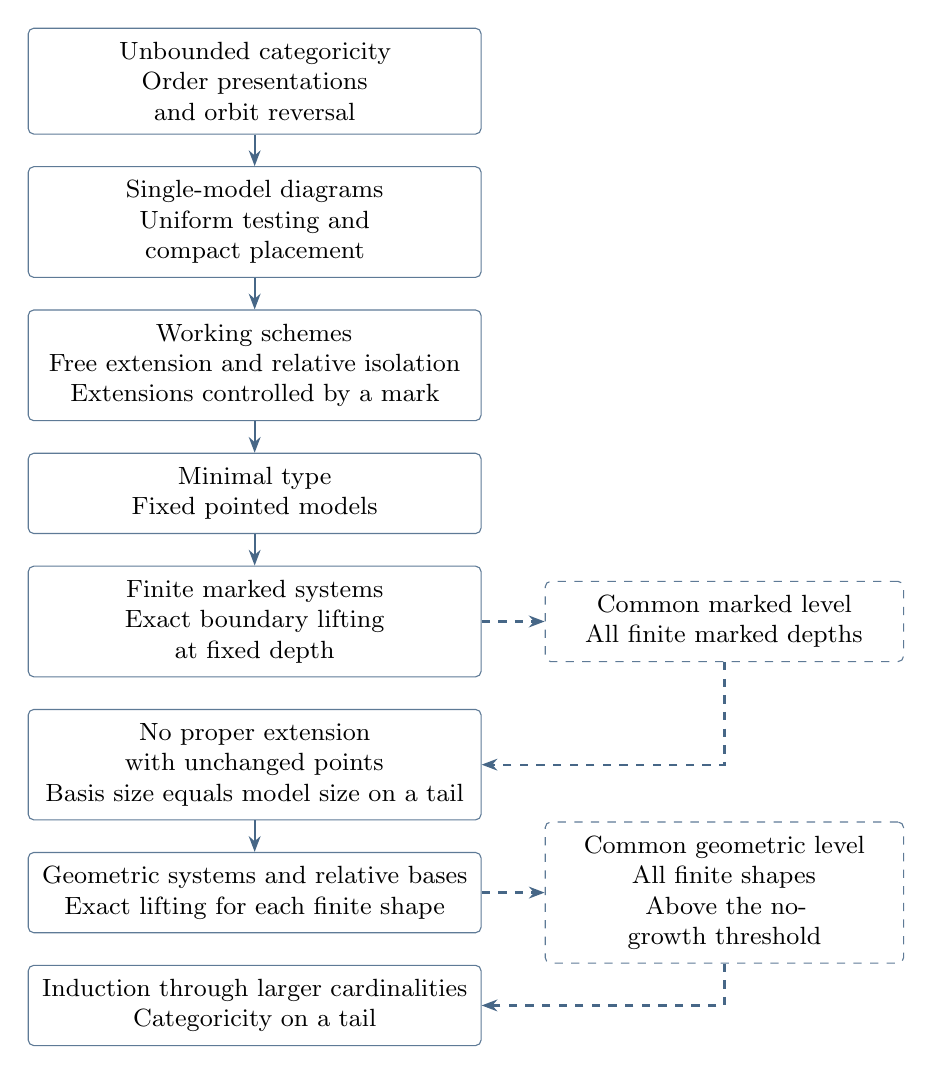
\begin{tikzpicture}[
  node distance=4mm and 8mm,
  box/.style={draw=linkblue!70,rounded corners=2pt,align=center,
    text width=5.4cm,minimum height=10mm,inner sep=5pt,font=\small},
  closure/.style={box,dashed,text width=4.2cm},
  arr/.style={-{Stealth[length=2mm]},draw=linkblue!80,thick}]
\node[box] (orders) {Unbounded categoricity\\Order presentations and orbit reversal};
\node[box,below=of orders] (diagrams) {Single-model diagrams\\Uniform testing and compact placement};
\node[box,below=of diagrams] (calculus) {Working schemes\\Free extension and relative isolation\\Extensions controlled by a mark};
\node[box,below=of calculus] (point) {Minimal type\\Fixed pointed models};
\node[box,below=of point] (marked) {Finite marked systems\\Exact boundary lifting\\at fixed depth};
\node[box,below=of marked] (growth) {No proper extension with unchanged points\\Basis size equals model size on a tail};
\node[box,below=of growth] (systems) {Geometric systems and relative bases\\Exact lifting for each finite shape};
\node[box,below=of systems] (tail) {Induction through larger cardinalities\\Categoricity on a tail};
\foreach \a/\b in {orders/diagrams,diagrams/calculus,calculus/point,
 point/marked,growth/systems}
  \draw[arr] (\a) -- (\b);
\node[closure,right=of marked] (markedclosure)
  {Common marked level\\All finite marked depths};
\draw[arr,dashed] (marked.east) -- (markedclosure.west);
\draw[arr,dashed] (markedclosure.south) |- (growth.east);
\node[closure,right=of systems] (geometricclosure)
  {Common geometric level\\All finite shapes\\Above the no-growth threshold};
\draw[arr,dashed] (systems.east) -- (geometricclosure.west);
\draw[arr,dashed] (geometricclosure.south) |- (tail.east);
\end{tikzpicture}
\caption{The qualitative proof, ordered by its principal dependencies.
The two dashed boxes are separate applications of
Section~\ref{close:section-uniform}. The first makes all finite marked
depths available for the no-growth argument over the fixed point. The
second is chosen after that argument
and supplies the starting cardinal for the final transfer. These
classes of common levels need not contain a tail. The small-code
reduction then gives the uniform threshold of
Theorem~\ref{main:uniform}.}
\label{fig:proof-route}
\end{figure}


\subsection{Conventions}

All size variables are cardinals unless explicitly called ordinals.
An assertion about bounded tuples at a level $\mu$ concerns tuples of
length strictly below $\mu$. Eligible working levels have countable
cofinality and are strong limits closed under the displayed bounds.
Whenever smaller adequate levels are needed cofinally below a working
level, that requirement is stated and included in the closure bookkeeping.
Automorphisms of an index order always mean automorphisms of its pure
linear order. Charts, auxiliary hulls, and basis choices are not added to
the structures whose isomorphisms are being compared.

\section{Set codes and models indexed by orders}
\label{found:section-reduction-orders}

We first separate the uniformity over AECs from the transfer argument for
one AEC. All directed families below are nonempty and set-indexed. We
begin by deriving the directed forms of the chain axioms in
Definition~\ref{main:aec}.

\begin{lemma}[Directed unions and coherent direct limits]
\label{found:directed-colimits}
If a nonempty set of models is directed under strong inclusion, its
union belongs to $\K$ and every member is strong in the union. If
every member is strong in a common model $N$, its union is strong in
$N$. More generally, a coherent diagram of strong maps indexed by a
nonempty directed partial order has a direct limit in $\K$, with
strong canonical maps. Every compatible family of strong maps from
the diagram into a model induces a strong map from the direct limit.
\end{lemma}

\begin{proof}
The union is a well-defined $\tau$-structure: finitely many
arguments are contained in one family member, and any two
choices of such a member agree after passing to a common
strong upper member. Here finitarity is used for functions
and relations alike.
We prove the union and common-upper-bound assertions together by
induction on the cardinality of the family. A finite directed
family has a member containing every other member, so its union is
that member. A countable directed family has a cofinal increasing
sequence: enumerate the family and successively choose a member
above the previous choice and the next enumerated member. The
chain axioms apply to this sequence, including their
common-upper-bound clause.

Suppose the family is indexed by a set $I$ of uncountable
cardinality $\kappa$, and the two assertions hold for smaller
families. Choose an operation assigning to each pair of indices
an index of a strong upper bound. Express $I$ as the union of an
increasing continuous sequence $(I_\alpha)_{\alpha<\cf(\kappa)}$
of nonempty subsets of size less than $\kappa$, each closed under
that operation. To obtain this sequence, enumerate $I$ by
$\kappa$, use a cofinal sequence of ordinals below $\kappa$
to specify the required initial segments, close each stage
under the binary operation by countably many iterations, and
take unions at limit stages. A union of fewer than
$\cf(\kappa)$ sets of size less than $\kappa$ still has size
less than $\kappa$; countable closure preserves the size of
each infinite stage. This construction also works when
$\kappa$ is a successor cardinal, using $\kappa$ many stages.

Let $U_\alpha$ be the union of the family on $I_\alpha$. The
induction hypothesis gives $U_\alpha\in\K$. For $\alpha<\beta$,
every member indexed by $I_\alpha$ is strong in $U_\beta$.
The inductive common-upper-bound assertion therefore gives
$U_\alpha\leq_\K U_\beta$. The chain axioms now give the
required union over $I$. If the original family is strong in
$N$, induction first gives $U_\alpha\leq_\K N$ for every
$\alpha$, and the chain common-upper-bound clause gives the
same conclusion for their union. This completes the induction.

For a diagram $(M_i,f_{ij})$ indexed by a directed partial order,
form the quotient of the disjoint union of its underlying sets
by
\[
(i,x)\sim(j,y)
\quad\Longleftrightarrow\quad
(\exists k\geq i,j)\ f_{ik}(x)=f_{jk}(y).
\]
Directedness and coherence make this an equivalence relation.
The canonical map from each $M_i$ is injective. Interpret any
finitary function or relation in a common later model containing
representatives of its arguments; coherence and the fact that
the maps are structure embeddings make this interpretation
well-defined. The images of the $M_i$ are models forming a
directed family of strong inclusions. The first assertion puts
their union, which is the quotient just constructed, in $\K$
and makes all canonical maps strong.

Finally, compatible strong maps $g_i:M_i\longrightarrow N$
induce a map on that quotient. It is injective: if two images
agree, compare their representatives in a common later $M_k$
and use injectivity of $g_k$. The same argument gives a
structure embedding. Its image is the directed union of the
strong submodels $g_i[M_i]$ of $N$, so the
common-upper-bound assertion makes the induced map strong.
The quotient construction also gives uniqueness, and hence
the stated direct-limit property.
\end{proof}

\begin{lemma}[Recovery from small models and pairs]
\label{found:small-code}
Fix an infinite cardinal $\lambda$ and a finitary language $\tau$ of
cardinality at most $\lambda$. An AEC in $\tau$ with
$\LS(\K)\leq\lambda$ is determined by its models of cardinality at most
$\lambda$ and its strong inclusions between such models, both taken up to
isomorphism. These data have a set code, and the recovered class and
strong-submodel relation are uniformly first-order definable in set
theory from that code.
\end{lemma}

\begin{proof}
Represent small structures on ordinals of cardinality at most $\lambda$.
Represent a small pair $M\subseteq N$ by such a representative for $N$
together with the distinguished subset that is the domain of $M$.
The possible structures and pairs form sets. A code specifies which
structure types and which pair types are allowed. Testing whether a
given small structure or pair has an allowed type is a set-theoretic
condition: quantify over the relevant isomorphisms.

For an actual $M\in\K$, let
\[
\mathcal D(M)=\{A\leq_\K M:\|A\|\leq\lambda\}.
\]
This is a set. It is nonempty by the LS axiom applied to the empty set,
and its union is $M$ by the LS axiom applied to singletons. If
$A,B\in\mathcal D(M)$, the LS axiom inside $M$ supplies a small strong
submodel containing $|A|\cup|B|$. Coherence makes both $A$ and $B$ strong
in that submodel. Thus $\mathcal D(M)$ is directed.

Conversely, suppose a structure $M$ is the union of a nonempty directed
family of small structures whose membership and pair inclusions are
allowed by the code of $\K$. These are actual members and strong
inclusions of $\K$, so the directed-union axiom gives $M\in\K$.
Consequently the following condition recovers membership, including for
structures not already assumed to belong to $\K$:
\begin{quote}
$M$ is a union of a nonempty directed family of allowed small models,
with all its directed inclusions allowed by the small-pair code.
\end{quote}

To recover the strong relation, require a directed presentation
$N=\bigcup\mathcal D$ of this kind and a nonempty directed subfamily
$\mathcal E\subseteq\mathcal D$ with $M=\bigcup\mathcal E$.
If $M\leq_\K N$, use $\mathcal D=\mathcal D(N)$ and
$\mathcal E=\mathcal D(M)$; transitivity makes the second a subfamily
of the first. In the reverse direction, every member of $\mathcal E$
is strong in $N$ by the union clause for $\mathcal D$. The
common-upper-bound clause for $\mathcal E$ then gives $M\leq_\K N$.

Each presentation can be quantified over as a set of substructures of
the structure being decoded. All the preceding conditions are thus
first-order set-theoretic formulas with the small code as parameter.
They recover both the class and the order, as asserted.
\end{proof}

The equivalence below is the usual Hanf-number reduction; compare
\cite[Remark~1.3]{VaseyUniversalI}. We spell out the set coding to make
the uniform quantifier explicit.

\begin{proposition}[The uniform reduction]
\label{found:uniform-reduction}
The uniform assertion in Theorem~\ref{main:uniform} is equivalent to
the following qualitative assertion:
\begin{quote}
Every AEC categorical in unboundedly many cardinals is categorical in
all cardinals above some bound depending on that AEC.
\end{quote}
\end{proposition}

\begin{proof}
At a fixed LS bound $\lambda$, the languages can be renamed into a
fixed set of symbols with specified finite arities. By
Lemma~\ref{found:small-code}, the possible AECs in those languages are
determined by members of a set of small codes. A code is valid exactly
when its decoded class and relation satisfy the AEC axioms with LS
bound $\lambda$. This is a first-order condition on the code, so the
valid codes form a set.

Assume the qualitative assertion. For each valid code $c$, its
categoricity spectrum is either bounded or unbounded. In the bounded
case choose the least infinite cardinal $b_c$ strictly above every
categoricity cardinal. In the unbounded case choose the least infinite
cardinal $b_c$ such that the decoded AEC is categorical in every
cardinal at least $b_c$. These choices are definable, and the second
choice exists by the qualitative assertion. Replacement bounds the
set of all $b_c$. Choose a cardinal $\mu(\lambda)\geq\lambda$ strictly
above that set of bounds. If an AEC with LS number at most $\lambda$
is categorical at some $\kappa\geq\mu(\lambda)$, its code cannot be
in the bounded-spectrum case. It is therefore categorical at every
$\kappa'\geq b_c$, in particular at every
$\kappa'\geq\mu(\lambda)$. This is exactly the same threshold in
the premise and conclusion.

Conversely, for an AEC categorical unboundedly often, apply the uniform
assertion with $\lambda=\LS(\K)$. Some categoricity cardinal crosses
the resulting threshold, and the asserted tail follows.
\end{proof}

\begin{remark}
Lemma~\ref{found:small-code} also supplies the usual ZFC interpretation
of quantification over AECs: one quantifies over their set codes and
uses the decoded class predicates. No choice of representatives from
a proper class and no class choice axiom is needed. Below we fix one
AEC categorical unboundedly often and write $\ell=\LS(\K)$. It has
arbitrarily large models because categoricity includes existence.
\end{remark}

\subsection{A finite-arity partition argument}

The following end-homogeneous argument belongs to classical partition
calculus; compare Erd\H{o}s and Rado
\cite[Theorem~39 and its corollary]{ErdosRado1956}.  We prove the
finite-arity form and bounds used by the order-template construction.

\begin{lemma}
\label{found:partition}
For infinite cardinals $\xi,\nu$ and a positive integer $k$, there is
an infinite cardinal $R_k(\xi,\nu)$ such that every coloring of the
$k$-element subsets of an ordinal of cardinality at least
$R_k(\xi,\nu)$ into $\xi$ colors has a homogeneous subset of
cardinality $\nu$. Finitely many specified arities can be made
homogeneous simultaneously by enlarging the initial cardinal.
\end{lemma}

\begin{proof}
For $k=1$, a set of cardinality greater than $\xi\cdot\nu$ cannot be
partitioned into $\xi$ sets all of cardinality less than $\nu$.
Suppose the assertion is known for $k$. Choose an infinite initial
ordinal $\alpha$ large enough for that $k$-ary assertion with target
$\nu$, and put $b=\xi^{|\alpha|}$. Consider a coloring $c$ of the
$(k+1)$-element subsets of an ordinal $\Omega$ with $|\Omega|>b$.

Construct a tree of residual subsets of $\Omega$ through height
$\alpha$. Its root is $\Omega$. At a nonempty node, name and remove
its least point $x$. The previously named points on its branch,
together with $x$, form an increasing sequence. Partition the
remaining residual set according to all values
\[
u\longmapsto c(s\cup\{u\}),
\qquad
s\text{ a $k$-subset of that sequence}.
\]
The nonempty parts are the children. At a limit height, a branch has
as its residual set the intersection of the earlier residual sets;
retain the node precisely when this intersection is nonempty.

At each node there are at most $|\alpha|$ coordinates to record and
hence at most $b$ children. The total number of possible nodes
through height $\alpha$ is at most
$b^{|\alpha|}=b$. This includes the limit nodes, which are specified
by their branches. At most $b$ points are removed as node labels.
Choose $u\in\Omega$ which is never removed. At every height it
belongs to one residual set; at limit heights it belongs to the
intersection on that branch. Consequently it determines a branch
with $\alpha$ named points and nonempty remainder.

For every $k$-subset $s$ of these named points, all later named points
give the same value of $c(s\cup\{x\})$: that value was fixed by the
partition immediately after the last point of $s$ was named.
Therefore $c$ on increasing $(k+1)$-tuples from the branch depends
only on their first $k$ entries. Apply the $k$-ary induction
hypothesis to this induced coloring on the branch. Its homogeneous
$\nu$-subset is homogeneous for $c$ as well. For example, the
recursion just proved allows
$R_{k+1}(\xi,\nu)=(\xi^{R_k(\xi,\nu)})^+$ after increasing the
initial $R_1$ as needed.

For a finite list of arities, work backward to choose a bound large
enough for the last desired thinning after all the earlier ones.
Successive thinning preserves homogeneity already obtained. This
proves the final assertion.
\end{proof}

\subsection{A fixed presentation on every order}

The construction is an Ehrenfeucht--Mostowski presentation
\cite{EhrenfeuchtMostowski1956}; for its AEC form compare
\cite[Definition~IV.0.8 and Claims~IV.0.9, IV.0.12]{Shelah2009}.
We include the finite-support construction in the label notation used below.

\begin{theorem}[Order presentation]
\label{found:order-template}
Suppose $\K$ has arbitrarily large models and $\LS(\K)=\ell$.
There are at most $\ell$ labels, each of positive finite arity, and a
functor $E$ from nonempty linear orders and order embeddings to
$\K$ and strong maps, with the following properties.
\begin{enumerate}
\item Every element of $E(I)$ is a label evaluated on an increasing
finite list from $I$. Equality and all structure relations and
function values are determined by the labels and the order/equality
pattern of the finitely many indices involved.
\item $E(I)$ contains distinct distinguished elements $(a_i)_{i\in I}$.
An order embedding $f:I\longrightarrow J$ sends $a_i$ to $a_{f(i)}$,
and its action on any labeled element is position substitution.
\item For every finite nonempty $s\subseteq I$, the elements labeled
on $s$ form a strong submodel $E_s(I)$ of cardinality at most $\ell$.
For $s\subseteq t$ these submodels are strongly included, and
$E(I)=\bigcup_s E_s(I)$.
\item $|I|\leq\|E(I)\|\leq |I|+\ell$. In particular, for every
infinite $\kappa\geq\ell$, $\K$ has a model of cardinality exactly
$\kappa$.
\end{enumerate}
Here a subpresentation is identified with its image under the
canonical strong map when an inclusion of underlying universes is
convenient.
\end{theorem}

\begin{proof}
Take an arbitrarily large $M\in\K$ and distinct elements
$(a_i)_{i\in A}$ indexed by a large ordinal $A$. Recursively on the
positive finite size of $s\subseteq A$, choose $M_s\leq_\K M$ of
cardinality at most $\ell$ containing the displayed elements on $s$
and every $M_t$ for nonempty $t\subsetneq s$. There are only finitely
many such $t$, so the LS axiom applies with bound $\ell$. Coherence
gives $M_t\leq_\K M_s$.

Choose a surjective enumeration
$(m_{s,\eta})_{\eta<\ell}$ of each $M_s$, allowing repetitions. If
$s=\{i_0<\cdots<i_{n-1}\}$, require $m_{s,j}=a_{i_j}$ for $j<n$.
For an $n$-element set $s$, its color is the complete atomic diagram,
including negations and equalities, of all the enumerations
\[
(m_{t,\eta})_{\eta<\ell},
\qquad \varnothing\ne t\subseteq s,
\]
with the subsets of $s$ named by their relative positions. This
diagram includes formulas involving entries from different
enumerations. There are at most $\ell$ names and atomic formulas
for each fixed $n$, so its possible colors belong to a fixed set of
cardinality at most $2^\ell$.

We choose colors $d_n$, for $n\geq1$, so that for every finite $n$
there are samples of arbitrarily large cardinality homogeneous in
colors $d_1,\ldots,d_n$. Suppose $d_1,\ldots,d_{n-1}$ have been
chosen with this property. For any prescribed target cardinal,
choose such a sample large enough for Lemma~\ref{found:partition}
at arity $n$ and thin it to an $n$-homogeneous set of the target
cardinality. The earlier colors are retained. If every possible
$n$-color supported only boundedly large such thinnings, the
supremum of the bounds over the set of colors would bound all
thinnings, a contradiction. Thus one color $d_n$ supports
arbitrarily large thinnings. It restricts on every smaller subset
to the previously chosen colors. This proves the recursion and
its coherence. It asserts finite-stage realizability in
arbitrarily large samples; it does not require an infinite
simultaneous homogeneous set inside one sample.

For a nonempty linear order $I$, introduce symbols $(s,\eta)$ for
each finite nonempty $s\subseteq I$ and $\eta<\ell$, with $s$
listed increasingly. Equate $(s,\eta)$ and $(t,\zeta)$ when the
color $d_{|s\cup t|}$ says that the corresponding entries are
equal. Coherence makes this independent of passage to a larger
finite set of indices. Reflexivity, symmetry, and transitivity
hold because any finite instance occurs in a realized color.
Form the quotient by this equivalence relation.

Interpret a relation on finitely many quotient elements in a
color on the union of their supports. For a function symbol,
evaluate it in the enumerated model on that union and use a name
for its value. All its arguments belong to that enumerated model,
and the model is a substructure, so the value has such a name.
Changing representatives or enlarging the finite support gives
the same quotient element by the complete atomic diagram and
coherence. A constant can be evaluated using any one nonempty
finite support. Two such evaluations agree in a color on their
union. Thus these rules define a $\tau$-structure $E(I)$.

Let $E_s(I)$ consist of the elements named by $(s,\eta)$,
$\eta<\ell$. The color $d_{|s|}$ makes this a full enumerated copy
of one of the actual models $M_s$ in a sample. Names with support
$t\subseteq s$ are included in this copy: their equalities with
names in the enumeration on $s$ were recorded. If $s\subseteq u$,
the pair $E_s(I)\subseteq E_u(I)$ is isomorphic to an actual pair
$M_s\leq_\K M_u$ from a realization of $d_{|u|}$. Isomorphism
invariance therefore makes the inclusion strong. The family of
these small models is directed and covers the constructed
structure. Its directed union belongs to $\K$, with all
$E_s(I)\leq_\K E(I)$.

For an order embedding $f:I\longrightarrow J$, substitution
$(s,\eta)\mapsto(f[s],\eta)$ respects every defining diagram and
every inequality of names. It therefore induces an embedding
$E(f):E(I)\longrightarrow E(J)$. On each finite-support model it
is an isomorphism onto $E_{f[s]}(J)\leq_\K E(J)$. The
common-upper-bound clause applied to their directed union shows
that the whole image is strong in $E(J)$. Substitution also
proves $E(\id)=\id$ and $E(g\circ f)=E(g)\circ E(f)$.

Define $a_i$ by the first designated name on the singleton $\{i\}$.
The recorded equalities identify this with the designated name
for $i$ on any larger finite support. Distinct indices give
distinct elements because every relevant sample had that
property. The labels are indexed by $(n,\eta)$ with $n\geq1$
finite and $\eta<\ell$, so there are at most $\ell$ of them.
Counting finite supports proves the upper bound on size, and the
distinct displayed elements prove the lower bound.
\end{proof}

\section{Reversing maps on bounded tuples}
\label{found:section-reversal}

Throughout this Section, $\K$ is categorical unboundedly often,
$\ell=\LS(\K)$, and $E$ is the presentation of
Theorem~\ref{found:order-template}. The aim is to reverse a strong
self-map on any one fixed bounded tuple in every sufficiently large
categoricity model. We first construct index orders with uniformly
controlled short-tuple orbits.  Homogeneous-order orbit bounds already
play a role in Shelah's work; compare \cite[IV.5.1]{Shelah2009}.
The alignment and elimination below establish the form needed at arbitrary
categoricity cardinals.

For comparison, \cite[Fact~1.4 and the discussion of Claim~1.5,
pp.~3--4]{BoneyVasey2015} records syntactic-characterization results
under exponentiation or cofinality conditions and a gap in the attempted
unrestricted extension. The bounded-tuple reversal needed here is proved
directly in Theorem~\ref{found:reversal}.

\subsection{Finite-support orders and their cuts}

\begin{definition}
\label{found:orders-definition}
For an infinite limit ordinal $\delta$, set
\[
\Gamma_\delta=\Z^{(\delta)},\qquad
H(\delta)=\Q^{(\Gamma_\delta)}.
\]
Parentheses denote finite support. Both groups are ordered by their
greatest differing coordinate. Write $e_\alpha$ for the integer basis
vector at $\alpha<\delta$ and $u_g$ for the rational basis vector at
$g\in\Gamma_\delta$. The rank of a nonzero vector is its greatest
support coordinate. Unless group operations are explicitly mentioned,
$H(\delta)$ is used as a pure linear order; in particular
$\Aut(H(\delta))$ means its order automorphism group.

A cut of an order $L$ is a partition $(L^-,L^+)$ with $L^-<L^+$.
It is an interior nonprincipal cut when both sides are nonempty,
$L^-$ has no greatest element, and $L^+$ has no least element. Its
two characters are $\cf(L^-)$ and $\ci(L^+)$. It is balanced if
these cardinals are equal. Cofinality and coinitiality here refer
to the indicated linear orders.
\end{definition}

\begin{lemma}
\label{found:order-basic}
The order $H(\delta)$ is dense without endpoints and has cardinality
$|\delta|$. Its points have character $\cf(\delta)$ on both sides.
All nonempty bounded open intervals have one order type. All left
rays have one order type, and all right rays have one order type.
An increasing map between ordinal position sets induces an order
embedding between the corresponding $\Gamma$ and $H$ orders by
moving positions and padding by zero. Each point of $H(\delta)$ has
a code using finitely many ordinal positions and integer and
rational coefficients; comparisons are determined by these discrete
coefficients and the order/equality pattern of the ordinal positions.
\end{lemma}

\begin{proof}
Finite-support counting gives
$|\Gamma_\delta|=|H(\delta)|=|\delta|$. The group
$\Gamma_\delta$ has least positive element $e_0$, so every $g$ has
predecessor $g-e_0$. Its cofinality and coinitiality are both
$\cf(\delta)$. Indeed, the vectors $e_\alpha$ for $\alpha$ in a
cofinal subset of $\delta$ are cofinal, and their negatives are
coinitial. The supports of fewer than $\cf(\delta)$ vectors are
bounded in $\delta$, so such a family is neither cofinal nor
coinitial.

The order $H(\delta)$ is a divisible nonzero ordered abelian group,
and hence is dense and has no endpoints. If $(g_i)$ is coinitial
in $\Gamma_\delta$, then $(u_{g_i})$ is coinitial in the positive
cone of $H(\delta)$: given a positive vector of rank $g$, choose
$g_i<g$. Conversely, the ranks of fewer than $\cf(\delta)$ positive
vectors have a strict lower bound in $\Gamma_\delta$, and a positive
basis vector at that lower rank lies below all of them. Thus the
positive cone has coinitiality $\cf(\delta)$. Translation and
negation give that character at every point on both sides.

Translations move points and therefore identify rays of a fixed
direction. We show that any positive vector can be sent to any
other by an increasing automorphism. First translate the index
group $\Gamma_\delta$ so that their greatest support coordinates
agree, say at $g$. Write the two vectors as
\[
a u_g+v,\qquad b u_g+w,
\qquad a,b\in\Q_{>0},\quad \rk(v),\rk(w)<g,
\]
allowing zero lower parts. Fix all other basis vectors and replace
$u_g$ by
\[
\frac ba u_g+\frac{w-v}{a}.
\]
This is an invertible triangular rational-linear map. It preserves
the sign of every nonzero vector, since it either fixes the greatest
nonzero coordinate or multiplies its coefficient by $b/a>0$.
It sends the first displayed vector to the second. Combining this
map with translations sends any ordered pair of distinct points to
any other such pair. Restricting gives the interval assertion.

Finally, an increasing map on ordinal positions preserves the
greatest differing position of two integer vectors. The induced
map on these integer vectors preserves the greatest differing
position of rational vectors as well. This proves the embedding
claim. Expanding the finitely many integer-vector positions used
by a rational vector gives the asserted finite code and comparison
rule.
\end{proof}

\begin{lemma}[Balance of cuts]
\label{found:balanced-cuts}
Every interior nonprincipal cut of $\Gamma_\delta$, and every such
cut of $H(\delta)$, is balanced.
\end{lemma}

\begin{proof}
First consider a cut $(L,R)$ of $\Gamma_\delta$. Among the ranks of
$r-l$, with $l\in L$ and $r\in R$, choose the least ordinal
$\alpha$. Fix one crossing pair of that rank and its common head
above $\alpha$. In that head, each fiber with a fixed integer
coefficient at $\alpha$ lies wholly on one side: a crossing pair
within a fiber would have smaller rank. The resulting cut in the
integer coefficients separates two adjacent integers. A point
with a head above the fixed head would exceed the fixed upper
point, and a point with a head below it would precede the fixed
lower point. The two bordering fibers are therefore cofinal
and coinitial toward the original cut, and their tails are
copies of $\Z^{(\alpha)}$. Their end
characters agree by negation in that tail group. The case
$\alpha=0$ would give a last lower and a first upper point, and
is excluded. This proves balance in $\Gamma_\delta$.

Now let $(L,R)$ be an interior nonprincipal cut of $H=H(\delta)$,
and put
\[
T=\{\rk(r-l):l\in L,\ r\in R\}\subseteq\Gamma_\delta.
\]
This is a final segment: from a crossing pair of rank $g$, subtract
a positive basis vector at any $h>g$ from its lower point. The new
pair still crosses and has rank $h$.

Suppose first that $T$ has a least member $g$. Fix a crossing head
above $g$. Every fiber with a fixed rational coefficient at $g$
lies on just one side of the cut. Otherwise a crossing difference
would have rank below $g$. The induced cut of $\Q$ is nonempty
and proper. If neither coefficient side has a nearest rational,
countable rational approximations are cofinal and coinitial in
the original cut. If the lower coefficients have a greatest
member, the entire fiber at that coefficient lies on the lower
side and is cofinal there. Its tail, supported below $g$, has
greatest available rank $g-e_0$, and the vectors
$n u_{g-e_0}$ and $-n u_{g-e_0}$ show that both its end characters
are $\aleph_0$. On the upper side, rational coefficients decreasing
to the greatest lower coefficient give coinitiality $\aleph_0$.
If instead the upper coefficients have a least member, the
reversed calculation gives cofinality and coinitiality
$\aleph_0$. These cases exhaust the rational cuts, so the original
cut is balanced.

Suppose that $T$ has no least member, and let
$\epsilon=\ci(T)$. Put $S=\Gamma_\delta\setminus T$ and let
$H_S$ be the subgroup supported on $S$. We prove that the lower
character is $\epsilon$ by separating two cases.

Assume there is $l\in L$ for which
\[
\{\rk(r-l):r\in R\}
\quad\text{is coinitial in }T.
\]
The coset $l+H_S$ is contained in $L$, since a crossing within it
would have rank in $S$. It is cofinal in $L$. In fact, if a point
$l'\in L$ lay above the entire coset, $l'-l$ would have positive
rank $h\in T$. Choose $r\in R$ with $\rk(r-l)<h$. Then
$r-l<l'-l$, contradicting $r>l'$. The set $S$ is nonempty, since
otherwise the cofinal coset would be the singleton $\{l\}$.
It has no greatest member: if $s$ were greatest, $s+e_0$ would
be the least member of $T$. Balance in $\Gamma_\delta$, applied
to $(S,T)$, gives $\cf(S)=\epsilon$. The cofinality of $H_S$ at
its upper end equals $\cf(S)$. A cofinal set of ranks gives
cofinal positive basis vectors, while fewer ranks are bounded
and cannot give a cofinal family of vectors. Hence
$\cf(L)=\epsilon$ in this case.

In the other case, each $l\in L$ has a bound $t_l\in T$ strictly
below all ranks $\rk(r-l)$, $r\in R$. Choose crossing pairs
$(l_i,r_i)$, $i<\epsilon$, whose ranks are coinitial in $T$.
For fixed $l\in L$, choose $i$ with
$\rk(r_i-l_i)\leq t_l$. If $l_i\leq l$, then
$0<r_i-l\leq r_i-l_i$, whence
$\rk(r_i-l)\leq\rk(r_i-l_i)\leq t_l$, a contradiction.
Thus $(l_i)_{i<\epsilon}$ is cofinal in $L$.
If fewer than $\epsilon$ points of $L$ were cofinal, their bounds
$t_l$ would have a common strict lower bound in $T$, since
$\epsilon=\ci(T)$. A crossing pair below that bound would have
its lower point above all those points by the same calculation.
This is impossible, proving $\cf(L)=\epsilon$.

Apply the proved lower-side calculation after negating the order
and exchanging $L$ and $R$. Negation preserves every difference
rank, so it has the same $T$ and $\epsilon$. It yields
$\ci(R)=\epsilon$. This proves balance also in the no-least-rank
case.
\end{proof}

\subsection{The orbit record of a short sequence}

For a subset $A$ of a linear order $L$ and a cut
$A=A^-\sqcup A^+$, including cuts with an empty side, define its
\emph{strict slot} by
\[
S_L(A^-,A^+)=\{x\in L\setminus A:A^-<x<A^+\}.
\]
Its occupancy is the assertion that this set is nonempty.
The order/equality diagram of a sequence identifies its distinct
entries and the cuts of their induced order, so the occupancy
data can be indexed without choosing an enumeration of the cuts.

\begin{lemma}[Segments approaching a small cut]
\label{found:cut-segments}
Let $L$ be a dense linear order without endpoints, all of whose
points have character $\kappa$ on both sides. Suppose all bounded
open intervals have one order type and every interior nonprincipal
cut is balanced. For every infinite regular $\epsilon<\kappa$,
the following segment types depend only on $\epsilon$ and the
indicated direction:
\[
[p,\mathfrak c)=\{x\in L^-_{\mathfrak c}:p\leq x\},
\qquad
(\mathfrak c,p]=\{x\in L^+_{\mathfrak c}:x\leq p\},
\]
where $\mathfrak c$ is an interior nonprincipal cut of balanced
character $\epsilon$ and $p$ belongs to the appropriate side.
The isomorphisms can be chosen to match the displayed endpoint.
\end{lemma}

\begin{proof}
We prove both directions simultaneously by induction on the
infinite regular cardinal $\epsilon$. Consider two lower-side
segments and choose strictly increasing sequences
$(p_i)_{i<\epsilon}$ and $(q_i)_{i<\epsilon}$ cofinal in their
respective cut sides, with the indicated endpoints at index zero.
At a stage $i<\epsilon$, fewer than $\epsilon$ preceding points
are not cofinal, so one can choose the next point above them and
above the next point of a fixed cofinal sequence. This gives the
required strictly increasing sequences.

Partition the first segment into blocks as follows:
\[
B_0=\{p_0\},\qquad B_{j+1}=(p_j,p_{j+1}].
\]
For a nonzero limit $i<\epsilon$, set
\[
D_i=\{x\in L:(\exists j<i)\ x\leq p_j\},\quad
U_i=L\setminus D_i,\quad
\mathfrak c_i=(D_i,U_i),\quad B_i=(\mathfrak c_i,p_i].
\]
The cut $\mathfrak c_i$ is interior and nonprincipal. Its lower
side has no greatest point and has cofinality $\cf(i)$: the
strictly increasing $i$-sequence is cofinal there, and any
smaller proposed cofinal family would give a cofinal set of
indices in $i$. Its upper side contains $p_i$. If that side had
a least point $u$, the earlier sequence would give
$\cf(L_{<u})=\cf(i)<\kappa$, contradicting point character.
Balance therefore gives $\mathfrak c_i$ character $\cf(i)$ on
both sides. Since $i<\epsilon$, this is a regular cardinal
strictly below $\epsilon$.

Make the corresponding blocks from the $q_i$. Successor blocks
are isomorphic by bounded-interval homogeneity, adjoining their
greatest points. At a nonzero limit index $i$, use the
\emph{upper-side} induction assertion at $\cf(i)$ to match the
blocks. Match the singleton blocks at zero. These are ordered
partitions of the two segments. Indeed, for any point in the
first segment take the least $i$ such that it is at most $p_i$;
the three cases for $i$ put it in exactly the block just
specified. Gluing the block maps proves the lower-side assertion.

For the upper-side assertion choose strictly decreasing
coinitial sequences. The blocks are $\{p_0\}$ and
$[p_{j+1},p_j)$ at successors. At a nonzero limit $i$, put
\[
V_i=\{x\in L:(\exists j<i)\ p_j\leq x\},\qquad
W_i=L\setminus V_i,\qquad \mathfrak d_i=(W_i,V_i).
\]
The set $V_i$ has no least point and has coinitiality
$\cf(i)$. The set $W_i$ contains $p_i$; if it had a
greatest point, that point's upper character would be
$\cf(i)<\kappa$. Thus $\mathfrak d_i$ is nonprincipal,
and balance gives character $\cf(i)$ on both sides.
The block at $i$ is $[p_i,\mathfrak d_i)$, to which the
\emph{lower-side} induction assertion at $\cf(i)$ applies.
The least index with $p_i\leq x$ verifies that these blocks,
in reverse index order, partition the upper-side segment.
For $\epsilon=\aleph_0$ there are no nonzero limit indices below
$\epsilon$, so this simultaneous induction starts with just the
successor blocks. All displayed endpoint points are matched.
\end{proof}

\begin{theorem}[Short-sequence order orbits]
\label{found:order-orbits}
Let $\delta$ be an infinite limit ordinal and let $\theta$ be an
infinite cardinal with $\theta<\cf(\delta)$. Two sequences of
length at most $\theta$ in $H(\delta)$ lie in the same
$\Aut(H(\delta))$-orbit if and only if they have the same
order/equality diagram and the same occupancies of all strict
slots over their distinct entries.
\end{theorem}

\begin{proof}
Necessity follows from preservation of order. For sufficiency,
the order/equality diagrams give an increasing bijection
$f:A\longrightarrow B$ between the sets of distinct entries,
matching the indexed sequences. We extend it separately on
each occupied slot.

Choose a point $p$ in a slot over $A=A^-\sqcup A^+$. The portion
of the slot at or below $p$ has one of three forms. If
$A^-=\varnothing$, it is $(-\infty,p]$. If $A^-$ has greatest
member $a$, it is $(a,p]$. Otherwise put
\[
D=\{x:(\exists a\in A^-)\ x\leq a\},\qquad U=H(\delta)\setminus D.
\]
The cut $(D,U)$ has no greatest lower point, has $p$ on its
upper side, and has lower character
$\cf(A^-)\leq\theta$. Its upper side has no first point,
since such a point would have character at most $\theta$.
By Lemma~\ref{found:balanced-cuts} this is an interior
nonprincipal cut of balanced character $\cf(A^-)$. The
slot portion is $((D,U),p]$.

In the first case its type is fixed by ray homogeneity; in the
second case by bounded-interval homogeneity; in the third case
by Lemma~\ref{found:cut-segments}. The portion at or above $p$
has the corresponding classification using $A^+$, a least
member when present, and otherwise $\ci(A^+)$. The same
descriptions show that the slot has neither endpoint.

The order map $f$ preserves which boundary case occurs and the
cofinality or coinitiality of the relevant part of $A$. Thus
the corresponding occupied slot over $B$ has matching two
halves. Choose an interior point $q$ there and match the two
halves with their common point $p$ sent to $q$. They glue to a
slot isomorphism. The occupancy assumption ensures that empty
slots also correspond. The entry sets and their occupied slots
partition the whole order. Choice for this set of slots and
gluing with $f$ produce an increasing bijection of
$H(\delta)$, as required.
\end{proof}

\subsection{Bounded names for model orbits}

We now pass from automorphisms of the index order to automorphisms of its
model.  At the cofinalities covered by the orbit theorem, a support record
determines a model orbit, but different records may determine the same
orbit.  Only a uniform upper bound on their number is needed for reversal.

Fix an infinite tuple length $\theta$. A presentation of a
$\theta$-tuple in $E(H(\delta))$ specifies its labels and their
finite index lists. Flatten those lists into an indexed sequence
of at most $\theta$ points of $H(\delta)$. Its \emph{presentation
record} consists of the labels, the order/equality diagram of
this flattened sequence, and all its slot occupancies.

\begin{lemma}[Uniform orbit bound]
\label{found:orbit-bound}
There is a fixed set $\mathcal R_\theta$ of possible presentation
records, depending only on $\ell$ and $\theta$, with
\[
|\mathcal R_\theta|\leq B(\ell,\theta):=2^{2^{\ell+\theta}}.
\]
For every categoricity cardinal
$\kappa\geq\max(\ell,\theta^+)$, the set of automorphism orbits of
$\theta$-tuples in its model has cardinality at most
$B(\ell,\theta)$. This applies also when $\kappa$ is singular.
If $|\delta|=\kappa$ and $\cf(\delta)>\theta$, each realized
record in $E(H(\delta))$ determines exactly one such model orbit.
\end{lemma}

\begin{proof}
The finitely many positions belonging to each tuple entry can
be indexed in $\theta\times\omega$. Choices of arities and
labels number at most $2^{\ell+\theta}$. The flattened
order/equality diagrams number at most $2^\theta$; their sets
of cuts have size at most $2^\theta$, and occupancy subsets
number at most $2^{2^\theta}$. The displayed generous bound
therefore bounds a universal record set.

For a fixed $\delta$ with $\cf(\delta)>\theta$, equal records
give an order automorphism matching the flattened lists by
Theorem~\ref{found:order-orbits}. Applying $E$ gives an
automorphism of the model matching the tuples. Hence a
realized record determines one model orbit. Every tuple has
a labeled presentation, so the number of orbits is bounded
by the number of records.

For any $\kappa\geq\max(\ell,\theta^+)$, the ordinal
$\delta=\kappa+\theta^+$, with ordinal addition here, has
cardinality $\kappa$ and cofinality $\theta^+$. The model
$E(H(\delta))$ has cardinality $\kappa$ and is therefore a
copy of the categoricity model. This proves the bound without
any condition on $\cf(\kappa)$.
\end{proof}

Choose a model $C_\kappa$ at each categoricity size needed in a
given set-sized construction. On its $\theta$-tuple orbits put
$p\longrightarrow r$ when some strong self-map sends a
representative of $p$ to a representative of $r$. This relation
is reflexive and transitive: compose maps after using an
automorphism to align the intermediate representatives.
Choose an injection of the orbit set into the fixed cardinal
$B=B(\ell,\theta)$, once for each $\kappa$. These are its
\emph{orbit names}. For any copy of $C_\kappa$, a tuple's
name is independent of the isomorphism used to $C_\kappa$,
because two such isomorphisms differ by an automorphism.

For a suitable $\delta$ of size $\kappa$, let $F_{\kappa,\delta}$
be the partial function from $\mathcal R_\theta$ to $B$ sending
each realized record to its orbit name. The \emph{profile}
of this presentation consists of its named arrow relation
and $F_{\kappa,\delta}$. The profiles belong to a fixed set
of cardinality at most $2^B$; in particular this bound is
independent of $\kappa$ and $\delta$.

\subsection{Preserving every short record in a small subpresentation}

\begin{lemma}[Closure of ordinal supports]
\label{found:ordinal-support-closure}
Let $\theta^+\leq a$ be infinite cardinals and let $\beta$ be
an ordinal of cofinality greater than $a$. Every subset
$S\subseteq\beta$ of size at most $a$ is contained in a set
$T_0\subseteq\beta$ of size at most $a$ with the following
property: for every $P\subseteq T_0$ of size at most $\theta$
and every finite tuple from $\beta$, there is a tuple from
$T_0$ having the same order/equality diagram over $P$.
Moreover $T_0$ is bounded in $\beta$ and has cofinality
greater than $\theta$ in its induced order.
\end{lemma}

\begin{proof}
Construct increasing sets $S_i\subseteq\beta$ for $i<\theta^+$,
starting with $S$. At a successor stage consider all strict
slots over the entire well-ordered set $S_i$. There are at
most $|S_i|+1\leq a$ of them. In each finite slot add every
point; in each infinite slot add a countably infinite subset.
Together with $S_i$ this realizes every finite order/equality
pattern over $S_i$ which occurs in $\beta$. At limits take
unions. The cardinality stays at most $a$ throughout.

Set $T_0=\bigcup_{i<\theta^+}S_i$. Every set
$P\subseteq T_0$ of size at most $\theta$ is contained in
some $S_i$, by regularity of $\theta^+$. For a given finite
tuple, keep any coordinates already in $S_i$ and match its
other coordinates in their respective slots using the next
stage. This proves the asserted property over $P$.
Since $|T_0|\leq a<\cf(\beta)$, $T_0$ is bounded in
$\beta$. Each $S_i$ is bounded too, and its uppermost slot
is infinite. The next stage therefore contains points above
all of $S_i$. Every at-most-$\theta$ subset of $T_0$ is
bounded in this way, proving $\cf(T_0)>\theta$.
\end{proof}

\begin{lemma}[Appending a long indecomposable segment]
\label{found:append-segment}
Under the hypotheses of Lemma~\ref{found:ordinal-support-closure},
suppose $\beta$ is additively indecomposable. Let $T_0$ be as
there, and let $\delta<\beta$ be additively indecomposable,
with $\otp(T_0)<\delta$ and $\cf(\delta)>\theta$.
Place a consecutive segment $J$ of order type $\delta$
strictly after $T_0$ in $\beta$, and set $T=T_0\cup J$.
Then $\otp(T)=\delta$, and $T$ has the same finite-pattern
matching property over its at-most-$\theta$ subsets.
Consequently $H(T)\subseteq H(\beta)$ computes correctly
the occupancies of every strict slot over any sequence of
at most $\theta$ of its points.
\end{lemma}

\begin{proof}
Choose $\alpha<\beta$ above $T_0$. Indecomposability of
$\beta$ gives $\alpha+\delta<\beta$, so
$J=[\alpha,\alpha+\delta)$ is available. Indecomposability
of $\delta$ gives $\otp(T_0)+\delta=\delta$.

Fix a parameter subset $P\subseteq T$ of size at most
$\theta$ and a finite tuple in $\beta$. Match the
coordinates below $\alpha$ into $T_0$ over $P\cap T_0$
using Lemma~\ref{found:ordinal-support-closure}. Keep
coordinates in $J$ fixed. The parameters in $J$, together
with these finitely many retained coordinates, are bounded
in $J$ because $\cf(\delta)>\theta$. Match all coordinates
at or beyond the end of $J$ by suitably many distinct
points of $J$ above that bound, retaining any repetitions.
The three portions stay in their correct mutual order,
and this gives the required finite tuple over $P$.

Here $\Gamma_T=\Z^{(T)}$ is identified with its image in
$\Gamma_\beta$, and $H(T)=\Q^{(\Gamma_T)}$ with its image
in $H(\beta)$. A sequence of at most $\theta$ points of
$H(T)$ uses at most $\theta$ ordinal positions in its
finite codes. A witness in $H(\beta)$ to an occupied
strict slot uses only finitely many additional ordinal
positions. Match those into $T$ over all the parameter
positions and retain the integer and rational
coefficients. Lemma~\ref{found:order-basic} makes every
comparison with the sequence unchanged. The resulting
point of $H(T)$ witnesses that slot. The reverse
implication follows from inclusion.
\end{proof}

\begin{proposition}[Alignment of model orbits]
\label{found:alignment}
Fix the record set and orbit naming at an infinite length
$\theta$. Let $a<\mu$ be categoricity cardinals with
$a\geq\max(\ell,\theta^+)$. Suppose the following data
have one common profile:
\begin{enumerate}
\item a presentation $E(H(\beta))$ of $C_\mu$, where
$\beta$ is additively indecomposable, $|\beta|=\mu$,
and $\cf(\beta)>a$;
\item presentations $E(H(\delta))$ of $C_a$ for a
cofinal subset of $a^+$ of additively indecomposable
ordinals $\delta$ of size $a$ and cofinality greater
than $\theta$.
\end{enumerate}
Then in any copy $N$ of $C_\mu$, every subset of size
at most $a$ is contained in $A\leq_\K N$ of size $a$
such that the orbit name of \emph{every} $\theta$-tuple
in $A$, computed as a tuple of $C_a$, is the same as
its name computed in $N$.
\end{proposition}

\begin{proof}
Identify $N$ with the presentation in the first item.
Represent the requested set by labeled elements and
collect the ordinal positions in the finite codes of
their indices. There are at most $a$ positions. Apply
Lemma~\ref{found:ordinal-support-closure} to obtain
$T_0$. Its order type is below $a^+$. Choose a
profile occurrence $\delta$ from the second item above
$\otp(T_0)$. Since $a^+\leq\cf(\beta)\leq\beta$ and
$\delta<a^+$, Lemma~\ref{found:append-segment} applies
and gives $T$ of order type $\delta$.

The subpresentation $A=E(H(T))$ is strong in $N$ and
has cardinality $a$. It contains the requested set.
For any $\theta$-tuple in $A$, use a labeled
presentation there. Its record is identical in
$E(H(T))$ and $E(H(\beta))$ by the last assertion of
Lemma~\ref{found:append-segment}. The order isomorphism
$\delta\cong T$ identifies its record in the former
with the same record for $E(H(\delta))$. The two
record-to-name functions belong to the common profile
and hence agree. This proves alignment simultaneously
for all $\theta$-tuples of $A$.
\end{proof}

\subsection{The elimination argument}

Alignment compares every short tuple in a small submodel with its image
in a larger model.  We now use repeated profiles at two categoricity sizes
to rule out an orbit arrow with no reverse.  The larger size will absorb
the cost of processing all tuples of the small model.

\begin{lemma}
\label{found:indecomposable-occurrences}
If $\kappa$ is an infinite cardinal and $\tau\leq\kappa$
is infinite regular, the additively indecomposable
ordinals $\delta<\kappa^+$ with $|\delta|=\kappa$ and
$\cf(\delta)=\tau$ are cofinal in $\kappa^+$.
\end{lemma}

\begin{proof}
Given $\eta<\kappa^+$, choose a limit ordinal
$\rho>\eta$ with $\kappa\leq\rho<\kappa^+$ and
$\cf(\rho)=\tau$, for example by appending an ordinal
segment of type $\tau$ beyond $\eta+\kappa$.
Set $\delta=\omega^\rho$. It is additively
indecomposable. A cofinal sequence of exponents gives
a cofinal sequence in $\omega^\rho$ by continuity of
exponentiation. Fewer than $\cf(\rho)$ ordinals below
$\omega^\rho$ have all their Cantor-normal-form
exponents bounded below $\rho$, and are therefore
bounded in $\omega^\rho$. This proves
$\cf(\delta)=\cf(\rho)=\tau$.
Every ordinal below $\omega^\rho$
has a finite Cantor normal form with exponents below
$\rho$. Thus $|\delta|\leq\max(\aleph_0,|\rho|)=\kappa$.
Since $\delta\geq\rho\geq\kappa$ and $\rho>\eta$,
we have $|\delta|=\kappa$, $\delta<\kappa^+$, and
$\delta>\eta$.
\end{proof}

\begin{theorem}[Eventual reversal at categoricity cardinals]
\label{found:reversal}
For each infinite cardinal $\theta$ there is a cardinal
$b_\K(\theta)$ such that, whenever
$\kappa\geq b_\K(\theta)$ is a categoricity cardinal,
$M\in\K$ has size $\kappa$, $f:M\longrightarrow M$
is strong, and $\bar a$ is a tuple of length at most
$\theta$ in $M$, there is a strong
$g:M\longrightarrow M$ with
\[
g(f(a_i))=a_i
\quad\text{for every coordinate }i.
\]
The bound concerns all sufficiently large categoricity
cardinals, of arbitrary cofinality. No equality of the
form $\kappa^\theta=\kappa$ is assumed.
\end{theorem}

\begin{proof}
It suffices to treat length exactly $\theta$; pad a
nonempty shorter tuple by repetitions, and use any
strong self-map for the empty tuple. In a categoricity
model, the asserted reversal is equivalent to symmetry
of the arrow relation on its $\theta$-tuple orbits.
Indeed a reverse orbit arrow can be precomposed and
postcomposed with automorphisms to match the particular
image tuple and original tuple. The converse follows
by applying reversal to a map witnessing an arrow.

Suppose that symmetry fails at unboundedly many
categoricity cardinals. Let $P$ be an infinite cardinal
bounding the profile palette; for example take $P=2^B$.
Choose a strictly increasing list of failing
categoricity cardinals $(\kappa_i)_{i<P^+}$. At each
step choose it large enough that there is an infinite
regular $\tau_i\leq\kappa_i$ exceeding $\ell$, $\theta$,
and every preceding $\kappa_j$, and that
\[
\kappa_i>P,\qquad
\kappa_i>\kappa_j^\theta\quad(j<i).
\]
Such choices are possible by unbounded failure: first
bound the set of preceding cardinals and their powers,
then choose a regular successor cardinal above the
first bounds and a failing cardinal beyond all of
them. This is a set-sized recursion.

At size $\kappa_i$, fix its orbit naming. By
Lemma~\ref{found:indecomposable-occurrences}, the
ordinals of size $\kappa_i$ and cofinality $\tau_i$
used there are cofinal in $\kappa_i^+$. One profile
occurs cofinally often among them: otherwise the
supremum of at most $P<\kappa_i^+$ bounded fibers
would be below the regular cardinal $\kappa_i^+$.
Since there are $P^+$ sizes and at most $P$ profiles,
choose two sizes $a<\mu$ with the same cofinally
recurring profile. They satisfy
\[
\theta^+\leq a,\qquad a^\theta\leq\mu,
\qquad \tau_\mu>a.
\]
Their common named arrow relation has $p\longrightarrow r$
but no $r\longrightarrow p$. Both names occur in
both sizes. Proposition~\ref{found:alignment} applies
inside every $\mu$-sized model, using any of its
cofinal profile occurrences.

We construct $\theta^+$ rounds of an increasing strong
chain of $\mu$-sized models. At the start of round
$i<\theta^+$, choose an aligned $a$-sized submodel
$A_i$ containing all previous $A_j$. This is possible
because their union has cardinality at most $a$.
They are all strong in the current large model, and
coherence will make $A_j\leq_\K A_i$ for $j<i$.

Enumerate all $\theta$-tuples of $A_i$, using
$a^\theta$ steps. At the step for a tuple $\bar u$,
if its current large-model orbit cannot reach $p$,
leave it as it is. If it can reach $p$, compose such
an arrow with $p\longrightarrow r$ and realize the
composite by a strong self-map of the current model.
Regard this map as an inclusion into an isomorphic
extension: rename its codomain so that the image of
each old element becomes that old element. With the
transported identification of the codomain, the
tuple now has name $r$. At every later large stage
its orbit remains unable to reach $p$. Otherwise
transitivity from $r$ would give $r\longrightarrow p$.
An orbit already unable to reach $p$ has the same
persistence property.

Take strong unions at every limit step, including
between rounds. The entire construction has at most
$\theta^+\cdot a^\theta\leq\mu$ many stages in
cardinality. Every large union therefore has size
$\mu$ and is a copy of $C_\mu$ by categoricity.
Every transition between such copies gives an arrow
of the common relation, so the persistence assertion
also holds at limit stages.

The aligned submodels form a strong increasing chain:
for $j<i$, their underlying sets are included and
both are strong in the large model at the start of
round $i$, so coherence applies. Its union
\[
A=\bigcup_{i<\theta^+}A_i
\]
belongs to $\K$, has cardinality $a$, and is a copy
of $C_a$. Any $\theta$-tuple of $A$ is contained
in some $A_i$, since $\cf(\theta^+)>\theta$. After
round $i$ it cannot reach $p$ in a large model.
At the next aligned small model its small orbit
has the same name, and therefore cannot reach $p$
in the common relation. The inclusion of that small
model into $A$ gives an arrow from this earlier
small orbit to its orbit in $A$. If the latter
could reach $p$, transitivity would contradict the
former exclusion. Thus no tuple in $A$ can have
an orbit reaching $p$.

But $A\cong C_a$, so the orbit named $p$ occurs in
$A$; it reaches itself by the identity map. This
contradiction proves that the failing categoricity
cardinals are bounded. A cardinal above their bound
is $b_\K(\theta)$, and the first paragraph gives
the claimed reversals, including all shorter lengths.
\end{proof}

\section{Stable diagrams and amalgamation at closed levels}
\label{lev:section-diagrams}

Throughout this section, \(\K\) is the AEC fixed after
Proposition~\ref{found:uniform-reduction}: it is categorical in unboundedly
many cardinals, and \(\ell=\LS(\K)\). We use the order presentation \(E\)
of Theorem~\ref{found:order-template}. A tuple may have any set as its
index set. Comparisons between tuples always specify the identification
of their index sets. Reindexing by an ordinal, padding, and repetitions
do not change any of the arguments below.

The goal is to turn bounded-tuple reversal into amalgamation at selected
levels.  We first stabilize tuple comparisons across categoricity sizes,
then use the order presentation to test and realize those comparisons
over an entire base.  Amalgamation will be a conclusion of this process.

\subsection{Stabilization of strong-map classes}

Fix an infinite cardinal \(\sigma\). At a categoricity cardinal
\(\kappa>\ell+\sigma\) where Theorem~\ref{found:reversal} holds for
\(\sigma\)-tuples, put
\[
 (M,a)\equiv^\sigma_\kappa(N,b)
 \quad\Longleftrightarrow\quad
 \text{some strong map }f:M\longrightarrow N\text{ satisfies }f(a)=b.
\]
Here \(\|M\|=\|N\|=\kappa\), and the lengths of the displayed
tuples are at most \(\sigma\).
This is an equivalence relation. Reflexivity is immediate. Categoricity
allows one to regard all the maps as maps between copies of one model;
reversal then gives symmetry, and composition gives transitivity.
Using structures with universe \(\kappa\), or one fixed representative
and its tuples, its classes form a set. Their number, for all the tuple
lengths under consideration, is bounded by the fixed cardinal supplied
by Lemma~\ref{found:orbit-bound}. Denote an infinite such bound by
\(B_\sigma\). It depends on \(\ell,\sigma\), not on \(\kappa\).

\begin{lemma}[Canonical classes above one categoricity size]
\label{lev:canonical-classes}
For \(\|N\|\ge\kappa\), a tuple \(a\) in \(N\) has a well-defined
\(\equiv^\sigma_\kappa\)-class: compute it in any strong
\(\kappa\)-submodel containing \(a\). Strong embeddings between models
of size at least \(\kappa\) preserve this class.
\end{lemma}

\begin{proof}
The downward LS axiom supplies the submodel, after adding
\(\kappa\) many elements to the requested set if necessary. If
\(M_0,M_1\le_\K N\) are two such submodels, apply LS to
\(|M_0|\cup|M_1|\). It gives \(M_2\le_\K N\) of size \(\kappa\)
containing both. Coherence gives \(M_i\le_\K M_2\). The two occurrences
of \(a\) therefore have the same class. For a strong embedding
\(f:N\to N'\), the image of a witnessing submodel is a strong
\(\kappa\)-submodel of \(N'\), so the same observation proves
preservation. All these comparisons take place inside a given ambient
model; no amalgamation property is used.
\end{proof}

\begin{proposition}[Stable diagrams]
\label{lev:stabilization}
There is a definable, nondecreasing cardinal function \(t\), with
\(t(\sigma)>\ell+\sigma\) a categoricity cardinal for every infinite
\(\sigma\), having the following properties.
\begin{enumerate}
\item Tuples of length at most \(\sigma\) in models of size at least
\(t(\sigma)\) have canonical diagrams. Equality of diagrams is
preserved by every strong embedding between such models, and there
are at most \(B_\sigma\) diagrams at these lengths.
\item Diagrams include atomic diagrams, respect reindexing and
restriction, and are compatible when the bound \(\sigma\) is
increased. We denote equality by \(D(a;M)=D(b;N)\), suppressing the
bound when it is understood.
\item If \(\kappa\ge t(\sigma)\) is a categoricity cardinal, equality
of diagrams between tuples in \(\kappa\)-models is implemented by
a strong map between those models.
\item A possible diagram of a pair of tuples \((a,c)\), of total
length at most \(\sigma\), can be realized over any tuple with the
diagram of \(a\) in any categoricity model of size at least
\(t(\sigma)\). ``Possible'' means that the diagram occurs in a
model in the domain of its definition.
\end{enumerate}
\end{proposition}

\begin{proof}
If \(\gamma\ge\kappa\) are categoricity cardinals above the reversal
threshold, Lemma~\ref{lev:canonical-classes} associates a
\(\kappa\)-class to every \(\gamma\)-class. This gives a projection
\(\pi_{\gamma\kappa}\), and these projections compose. They are
surjective. Indeed, a \(\kappa\)-model is isomorphic to \(E(I)\) for
\(|I|=\kappa\); extend \(I\) to an order of size \(\gamma\) and use
the strong order map. Every tuple class in the smaller model then
occurs in the larger one. This argument supplies the needed extension
without a no-maximal-model assumption.

These projections are eventually all bijective. Otherwise, construct
a sequence of categoricity cardinals with more than \(B_\sigma\)
successive noninjective projections, and choose one final
categoricity cardinal \(\rho\) above the entire sequence. For each
noninjective projection, surjectivity supplies a pair of
\(\rho\)-classes which agree when projected to the earlier stage and
differ when projected to the later stage. Pairs selected at distinct
stages are distinct: after a pair has separated it remains separated
under every later refinement. This gives more than
\(B_\sigma\) pairs from a set of size at most \(B_\sigma\), a
contradiction. The construction uses only a set-length sequence of
cardinals and choices from sets.

Choose a categoricity cardinal \(c_\sigma\) beyond this stabilization
and reversal threshold. The canonical \(c_\sigma\)-class defines
the desired diagram on models of size at least \(c_\sigma\).
The bijective projections show that its equality can equally be
computed at every later categoricity cardinal. If two tuple bounds
are used, compare them at a categoricity cardinal above both
thresholds. Restriction of strong maps then gives the same
restricted equivalence. Atomic formulas and their negations are
preserved because strong maps are structure embeddings.

For definiteness, thresholds can be chosen as least cardinals having
the stated eventual properties. Choose \(t(\sigma)\) to be the
least categoricity cardinal strictly above \(\ell+\sigma\) and
above all the thresholds \(c_\tau\) for infinite \(\tau\le\sigma\).
This is a nondecreasing definable function. The preceding arguments
prove the first three assertions.

For the fourth, first put a realization of \((a,c)\) into a strong
\(c_\sigma\)-submodel. If the originally chosen ambient size is
smaller than a desired target categoricity size, this categorical
submodel can be extended to that size by the order presentation.
If the original ambient size is larger, LS gives a submodel of the
desired size containing the realization. Thus the joint diagram
has a realization in a model of the target categoricity size.
Apply the third assertion to the first tuple and the specified tuple
in the target. The resulting strong map transports the whole
realization as required.
\end{proof}

\begin{proposition}[Categoricity at countably cofinal closure points]
\label{lev:closure-categoricity}
Suppose \(\zeta>\ell\) is an infinite cardinal of countable
cofinality and
\[
 t(\sigma)<\zeta\qquad\text{for every infinite }\sigma<\zeta.
\]
Then \(\K\) is categorical in \(\zeta\). Moreover any diagram match
between bounded tuples in two \(\zeta\)-models extends to an
isomorphism between those models. Here and throughout the paper,
bounded at a level means of cardinality strictly less than that level.
\end{proposition}

\begin{proof}
Existence follows from \(E(I)\) for \(|I|=\zeta\). Let \(M,N\)
have size \(\zeta\), and choose countable increasing exhaustions of
their underlying sets by sets of size less than \(\zeta\).
Start with the prescribed bounded diagram match, or with the empty
match. At a forward step, enumerate together the current source
tuple and the next part of the exhaustion of \(M\). Its length and
the length of the current target tuple are bounded by an infinite
\(\sigma<\zeta\). Put the data on each side inside a strong
submodel of size \(t(\sigma)<\zeta\). Their current tuples have
the same diagram. Proposition~\ref{lev:stabilization} gives a
strong map of these submodels matching those tuples. Its values
on the new entries extend the match, and the enlarged tuples
again have equal diagrams. At the next step interchange \(M,N\).

Only finitely many previously chosen bounded tuples are used at
each step, so their combined length stays below \(\zeta\).
The union of the countable sequence of partial matches is a
bijection \(|M|\to|N|\). Every finite tuple and every value of a
finitary function occur at some step, where the atomic diagram
is preserved. The bijection is therefore a structure isomorphism.
\end{proof}

The closure cardinals in Proposition~\ref{lev:closure-categoricity}
are unbounded. For example, starting above any specified cardinal,
choose a strictly increasing sequence \((\alpha_n:n<\omega)\)
such that \(\alpha_{n+1}\) exceeds all \(t(\sigma)\) for
\(\sigma\le\alpha_n\). Its supremum has the required closure and
countable cofinality. Including \(2^{\alpha_n}\) in these requirements
makes the supremum a strong limit. We will use these stronger
closure points below.

\subsection{Natural diagrams and interchange of blocks}

\begin{definition}[Natural and placed diagrams]
\label{lev:natural-diagrams}
Consider a set-sized list of terms in an order presentation. Each
term consists of a label and an increasing finite list of positions.
Extend the order to size at least the threshold for the list and
compute its diagram there. The result is its \emph{natural diagram}.
If \(A=E(I)\), a \emph{placement} of an additional tuple \(d\)
over \(A\) is a labeled representation in an order extension of
\(I\), retaining the positions and chosen representations of the
parameters in \(A\). Its \emph{placed comparison over \(A\)} is
the natural diagram of \((d,a_A)\), where \(a_A\) is a fixed
enumeration of \(A\).
\end{definition}

The natural diagram is independent of the extension used. Indeed,
linear orders amalgamate over a common suborder: for each cut of
the suborder, place the remaining portions of the two orders in
that cut while preserving each portion's order. Extending the
amalgam further if necessary gives a common sufficiently large
presentation. Strong order maps and
Proposition~\ref{lev:stabilization} identify the two diagrams.
The same argument shows that only the labels and the joint
order/equality pattern of their supports matter. All diagrams
with parameters use matching parameter enumerations. One may
instead list all labels on the base order, allowing repetitions:
restriction gives an enumeration of the elements, and reinserting
the repetitions is forced by their equalities.

A placed comparison over a whole \(\mu\)-model is evaluated in a
sufficiently large presentation. It is not, by this definition,
an assertion that the original \(\mu\)-model itself lies above the
threshold for diagrams of length \(\mu\).

\begin{lemma}[Orbits over parameters]
\label{lev:parameter-orbits}
Let \(\sigma\) be infinite and suppose
\[
 \chi^\sigma=\chi,
 \qquad \chi\ge \ell+2^{2^\sigma}.
\]
At every sufficiently large categoricity cardinal, there are at
most \(\chi\) automorphism orbits of \(\sigma\)-tuples over any
specified set of at most \(\chi\) parameters.
\end{lemma}

\begin{proof}
Present the categoricity model as \(E(H(\delta))\), choosing
\(|\delta|\) to be its cardinality and \(\cf(\delta)>\chi\).
This is possible at every sufficiently large cardinal, including
singular cardinals. Fix term representations of the parameters,
and let \(S\subseteq H(\delta)\) be their support set. Its size
is at most \(\chi\). Every member of \(S\) is coded by a finite
list of ordinals and integer and rational coefficients. The union
of its ordinal supports consequently also has size at most
\(\chi\).

For one further position, its finite ordinal support has at most
\(\chi\) possible order/equality patterns over these old ordinal
supports. The discrete coefficients contribute only countably
many choices for each finite code. Such a pattern determines
all comparisons of the new position with \(S\). For at most
\(\sigma\) new positions, include their mutual comparisons,
their identifications with old positions, and the term labels.
There are at most \(\chi^\sigma=\chi\) choices so far.

To apply Theorem~\ref{found:order-orbits}, also record which strict
slots over the old and new positions are realized in
\(H(\delta)\). The old support \(S\) is fixed. A slot over \(S\)
not containing a new position is unchanged. At most \(\sigma\)
old slots contain new positions, and inside each there are at
most \(2^\sigma\) cuts of the new support to test. The new flags
therefore have at most \(2^{2^\sigma}\le\chi\) possible values.
The full record has at most \(\chi\) possibilities.

The combined list of old and new positions has size at most
\(\chi<\cf(\delta)\). Theorem~\ref{found:order-orbits} extends
equality of full records to an order automorphism fixing \(S\)
pointwise. Its induced automorphism of the presentation fixes
the parameters and matches the tuples. Thus the number of
structure-automorphism orbits is at most the number of records.
\end{proof}

\begin{lemma}[Disjoint block transpositions]
\label{lev:block-transpositions}
Take two set-sized families of labeled terms. In disjoint convex
regions of their joint support order, suppose each region consists
of two adjacent blocks, one used only by the first family and one
only by the second. Interchange the blocks in every such region,
retaining their internal orders and all positions outside the
regions. The joint natural diagram is unchanged.
\end{lemma}

\begin{proof}
Suppose the original and modified diagrams were different. Let
\(\sigma\) bound the two lists, their supports, and the shared
positions. Choose \(\chi\ge\ell+2^{2^\sigma}\) with
\(\chi^\sigma=\chi\), for instance by taking a sufficiently
large power of two.

In each region repeat the pair of blocks along an arbitrary
linear order \(L\). If the first family's block was on the left,
use the order \(L\) for the repetitions; if it was on the right,
use the reverse of \(L\). Write \(d_i\) for the first-family
tuple using the blocks at index \(i\), and \(e_j\) for the
second-family tuple using the blocks at index \(j\); retain all
the shared positions outside the regions. For \(i<j\), the
diagram of \((d_i,e_j)\) is the original one, and for \(i>j\)
it is the modified one. Comparisons within either family and
across distinct regions do not change.

Let \(\epsilon\) be the least infinite cardinal satisfying
\(2^\epsilon>\chi\). The binary tree \(2^{<\epsilon}\) has
at most \(\chi\) nodes: for \(\alpha<\epsilon\) each level has
size at most \(\chi\), and \(\epsilon\le\chi\). Give it
lexicographically ordered divider points, one between the two
successor subtrees at each node. Explicitly, encode branch
digits by \(-1,1\), and encode the divider at a node \(s\)
by the sequence \(s\) followed by \(0\), using
\(-1<0<1\) in lexicographic comparison. Adjoin one point for every
branch in \(2^\epsilon\). Distinct branch points determine
distinct strict cuts over the divider points. Use this as the
order \(L\).

The tuples \(e_j\) at the divider indices, together with the
fixed shared data, use at most \(\chi\) parameters. If two
branch-indexed tuples \(d_i\) were in the same automorphism
orbit over these parameters, their diagrams with every divider
tuple would agree. A divider between the two branches gives
the two different diagrams, a contradiction. Hence there are
more than \(\chi\) such orbits. Pad the constructed order to a
sufficiently large categoricity size and apply
Lemma~\ref{lev:parameter-orbits}. This is impossible.
\end{proof}

\subsection{Bounded tests over a well-ordered presentation}

The next elementary set-theoretic observation will also be used for
the more elaborate layouts of later sections.

\begin{lemma}[Ordinal-vector witnesses]
\label{lev:ordinal-vectors}
Let \(C\) be a set, and let \(U\) be a definable class of functions
\(C\to\Ord\), with fixed set parameters allowed in its definition.
There is a set \(U_0\subseteq U\) such that each \(u\in U\)
dominates some \(v\in U_0\) coordinatewise.
\end{lemma}

\begin{proof}
The assertion is immediate if \(C\) is empty or \(U\) is empty.
Well-order \(C\), and suppose no such set exists. For every
ordinal \(\beta\), the set \(U\cap V_\beta\) fails to generate
\(U\) upwards. There is therefore an element of \(U\) which
dominates none of its members. Let \(h(\beta)>\beta\) be the
least ordinal such that one such witness lies in \(V_{h(\beta)}\).
This is a definable ordinal function.

Take an ordinal length \(\lambda\) satisfying the partition
relation for pairs, \(|C|\) colors, and an infinite homogeneous
set, supplied by Lemma~\ref{found:partition}. Define increasing
ordinals \(\beta_i\), for \(i\le\lambda\), recursively, with
\(\beta_{i+1}>h(\beta_i)\) and with limit values above all earlier
values. Choice for a set-indexed collection of nonempty subsets
of \(V_{\beta_\lambda}\) now selects witnesses \(u_i\) which
dominate no member of \(U\cap V_{\beta_i}\), for \(i<\lambda\).
For \(i<j\), we have \(u_i\in V_{\beta_j}\), so some coordinate
satisfies \(u_i(c)>u_j(c)\). Color the pair \(i<j\) by the first
such coordinate in the fixed well-order of \(C\). An infinite
homogeneous set yields an infinite strictly decreasing sequence
of ordinals in that coordinate. This contradiction proves the
claim. The rank bounding above ensures that only ordinary
set-sized Choice, not a choice principle for proper classes,
was used.
\end{proof}

\begin{proposition}[Uniform testing of placed comparisons]
\label{lev:testing}
There is a definable nondecreasing infinite cardinal function
\(g\), depending on \(\K\) and its fixed presentation, such that
the following holds. If \(I\) is an infinite well-order, \(A=E(I)\), and
two placements of a tuple of length at most \(\sigma\) have
different placed comparisons over \(A\), then their natural
diagrams already differ over a subset of \(A\) of size at most
\(g(\sigma)\). The bound is independent of \(|I|\).
\end{proposition}

\begin{proof}
Amalgamate the two support orders over \(I\), and let \(T\)
be the union of the supports of the two added tuples. Its size
is at most \(\sigma\). Freeze its order, the labels and supports
of the two tuples, and the subset of its positions which belong
to \(I\). Up to a relabeling on a fixed set of size at most
\(\sigma\), these frozen data range over a set.

For fixed frozen data, each component of \(I\setminus T\) in
a strict slot over \(T\) is well-ordered. Record its ordinal
length. The set of slots is fixed, so these lengths form an
ordinal vector. Restrict attention to the vectors that give
valid configurations and for which the two placed comparisons
are unequal. This is a definable class: order presentations
and diagrams are defined from set codes, and diagrams of any
specified set length can be evaluated above their thresholds.

Coordinatewise domination gives an order embedding of the
smaller configuration into the larger one, fixing \(T\) and
preserving the base positions. Natural diagrams respect these
embeddings. Thus a valid smaller unequal configuration remains
a witness in any dominating valid configuration. Apply
Lemma~\ref{lev:ordinal-vectors} to this class, obtaining a set
of valid witnesses. Equivalently one could apply it to the
upward closure and select its generators from valid
configurations; no assertion that arbitrary vectors themselves
describe well-orders is required.

Bound the sizes of the base orders in this set of witnesses.
An embedded witness uses only that bounded number of old
positions. All labels on these positions give at most their
cardinality plus \(\ell\) elements of \(A\), and the diagrams
of the two added tuples with these elements are unequal.
Taking a cardinal bound over the set of frozen data gives
\(g(\sigma)\). Increasing it to an infinite nondecreasing
function causes no change in the assertion. When a witness
uses only finitely many positions, ``all labels'' simply means
their evaluated terms; no assertion about membership of a
finite-order presentation in \(\K\) is needed.
\end{proof}

\begin{proposition}[Compact placement]
\label{lev:compact-placement}
Let \(A=E(I)\), where \(I\) is an infinite well-order, and let
\(\chi>\ell+\sigma\) satisfy \(\chi^\sigma=\chi\). Suppose that
for every \(X\subseteq A\) of size at most \(\chi\) a possible
joint diagram \(q_X(d,X)\) is prescribed, where \(d\) has length
at most \(\sigma\). Assume these prescriptions restrict
coherently and that their parameter diagrams are the natural
ones of \(X\). Then one placement of \(d\) over \(I\) realizes
all the prescriptions.
\end{proposition}

\begin{proof}
Fix one term representation per parameter in \(A\). Write
\(S_X\subseteq I\) for the supports of \(X\). For one set
\(X\), its prescription has a placement. To see this, extend
\(I\) to a sufficiently large categoricity size and use
Proposition~\ref{lev:stabilization} to realize the possible
joint diagram over the actual parameter tuple. The realization
has term representations in that presentation.

A support profile over \(X\) records the labels for \(d\),
its formal support order \(T_0\) of size at most \(\sigma\),
and comparisons and coincidences with \(S_X\). A well-order
of size at most \(\chi\) has at most \(\chi\) cuts. Hence
there are at most \(\chi^\sigma=\chi\) profiles. The positions
of \(T_0\) in one strict slot over \(S_X\) form a cluster.
Each profile has a continuation over \(I\) which leaves
every such cluster intact: insert the cluster at a single
cut of \(I\) extending its specified cut over \(S_X\).

Call a hit of a new parameter support on \(T_0\), or the
separation of two positions in one cluster by a new parameter
support, a new event. For \(X'\supseteq X\), all continuations
of a profile with no new event over \(S_{X'}\) have the same
natural diagram over \(X'\). Within each old slot, the whole
cluster can only change its position across a block of new
parameter positions. The slots are disjoint, so
Lemma~\ref{lev:block-transpositions} applies simultaneously.

Suppose no placement solves all the prescriptions. Start with
any \(X_0\) of size at most \(\chi\). Given \(X_i\), choose
for every profile over \(X_i\) a continuation with no new
event over all of \(I\). It fails a prescription on some set
of at most \(\chi\) parameters. Adjoin one such failing set
for each profile to obtain \(X_{i+1}\). At limits take unions,
and carry out \(\sigma^+\) stages. Every set constructed,
including \(X_* = \bigcup_{i<\sigma^+}X_i\), has size at most
\(\chi\), because \(\sigma^+\le\chi\).

Take a placement realizing \(q_{X_*}\). At each stage its
profile over \(X_i\) was considered. If it had no new event
between \(S_{X_i}\) and \(S_{X_{i+1}}\), the preceding
no-event comparison would identify its diagram on the
selected failing set with that of the chosen continuation.
This contradicts its realization of \(q_{X_*}\). Thus it
has a new event at every stage. A support position can be
newly hit only once, and a pair can be newly separated only
once. There are at most \(\sigma+\sigma^2=\sigma\) such
events. They cannot occur at \(\sigma^+\) different stages.
\end{proof}

\begin{lemma}[Unique lifts of bounded diagrams]
\label{lev:placed-lifts}
Let \(\mu>\ell\) be a strong-limit cardinal of countable
cofinality strictly closed below itself under \(t\) and \(g\).
Let \(A\le_\K B\) have size \(\mu\), and identify
\(A=E(I)\) for a well-order \(I\) of size \(\mu\). For a
tuple \(d\) in \(B\) of length at most \(\sigma<\mu\), the
diagrams
\[
 D(d,X;B),\qquad X\subseteq A,\quad |X|<\mu,
\]
lift to one placed comparison over all of \(A\), uniquely
as a comparison diagram. Restricting a lifted tuple gives
the lift of its restricted diagram.
\end{lemma}

\begin{proof}
The displayed bounded diagrams are defined, since their
thresholds lie below \(\mu\), and they agree on the parameters
with the natural diagrams. For every sufficiently large
\(\chi<\mu\) with \(\chi^\sigma=\chi\),
Proposition~\ref{lev:compact-placement} gives a placement
realizing the tests of size at most \(\chi\). Such \(\chi\)
are cofinal below \(\mu\): use \(\chi=2^\alpha\) for
\(\sigma\le\alpha<\mu\), enlarging \(\alpha\) as necessary.

Once \(\chi\ge g(\sigma)\), any two resulting placements
have the same full comparison by Proposition~\ref{lev:testing}.
Fix one of them. Every bounded test is covered by a larger
choice of \(\chi\), whose placement has that same full
comparison. The fixed placement consequently realizes every
bounded test. The same argument gives uniqueness. A
restriction realizes the restricted tests and hence, by
uniqueness, is their lift.
\end{proof}

\subsection{Amalgamation and type counts}

\begin{theorem}[Amalgamation at closed levels]
\label{lev:amalgamation}
There is an unbounded class of strong-limit cardinals \(\mu\)
of countable cofinality with the following properties.
\begin{enumerate}
\item \(\K\) is categorical in \(\mu\), and any two
\(\mu\)-sized strong extensions of a \(\mu\)-model have a
strong amalgam of size \(\mu\).
\item If \(A\le_\K B_0,B_1\) all have size \(\mu\), and
\(d_i\in B_i\) are tuples of the same length at most
\(\sigma<\mu\), there is such an amalgam identifying
\(d_0\) with \(d_1\) if and only if
\[
 D(d_0,X;B_0)=D(d_1,X;B_1)
 \quad\text{for every }X\subseteq A,
 \quad |X|\le g(\sigma).
\]
\item There are at most \(\mu\) singleton types over each
\(\mu\)-model, where type means identification in an amalgam
over that model.
\end{enumerate}
One may take every sufficiently large strong-limit cardinal
of countable cofinality strictly closed under \(t\) and \(g\).
\end{theorem}

\begin{proof}
Such levels are unbounded by the countable closure construction
following Proposition~\ref{lev:closure-categoricity}.
Categoricity at them has already been proved. Identify a
given base with \(A=E(I)\), where \(I\) is a well-order of
size \(\mu\). Extend \(I\) to an order \(J\) whose cardinality
\(\gamma\) is a categoricity cardinal at least \(t(\mu)\),
and let \(G=E(J)\). Thus \(A\) is strongly included in its
specified position in \(G\).

We show that every \(\mu\)-sized strong extension \(B\) of
\(A\) embeds strongly into \(G\) over \(A\). Choose
\(M_n\le_\K B\), increasing with union \(B\), with
\(\|M_n\|<\mu\). This follows by LS from a countable
exhaustion of \(B\), containing the preceding submodel at
each step; coherence makes the chain strong. Choose compatible
enumerations \(d_n\) of these models, so that each earlier
list is a sublist of the next.

Lemma~\ref{lev:placed-lifts} assigns coherent placed comparisons
to \((d_n,A)\). Each is realized over \(A\) in \(G\), and
the realizations can retain the previous assignments. More
explicitly, realize the corresponding term pattern in an
order extension of size \(\gamma\). Its parameter tuple
\(A\), and then its tuple \((A,d_{n-1})\), have the same
diagram as the already assigned ones. Their length is at
most \(\mu\), so Proposition~\ref{lev:stabilization} at
\(\gamma\ge t(\mu)\) supplies the strong map realizing the
new list while fixing these previous data.

It remains to verify strongness of the copied small models;
atomic agreement by itself would not suffice. Fix \(n\),
and bound the length of \(d_n\) by an infinite
\(\sigma_n<\mu\). Choose the categoricity cardinal
\(\rho=t(\sigma_n)<\mu\). LS puts the original enumeration
inside \(B_n'\le_\K B\) of size \(\rho\), and the copied
enumeration inside \(G_n'\le_\K G\) of that size. Coherence
gives \(M_n\le_\K B_n'\). The copied and original lists
have the same bounded diagram; Proposition~\ref{lev:stabilization}
gives a strong map \(B_n'\to G_n'\) with exactly the prescribed
values on \(d_n\). Its restriction shows that the copied
\(M_n\) is a strong submodel of \(G\).

The copied models are nested, and coherence makes their
inclusions strong. Their union is a strong submodel of \(G\)
by the chain and common-upper-bound axioms. It is the image
of an embedding of \(B\). Every element of \(A\) eventually
occurs in some \(d_n\), and its equality with that parameter
is part of the lifted comparison. The embedding therefore
fixes \(A\). Performing this construction for \(B_0,B_1\)
in the same \(G\) gives an amalgam. LS supplies a strong
\(\mu\)-submodel of \(G\) containing both images; coherence
makes it a strong amalgam of the required size.

For the second assertion, any identifying amalgam preserves
the displayed bounded diagrams, giving necessity. Conversely,
Proposition~\ref{lev:testing} identifies the placed lifts
of \(d_0,d_1\) over \(A\). Realize this common lift once
in \(G\). On each side start the preceding countable
construction with the specified tuple already assigned,
and choose every small-model enumeration to contain that
tuple. Homogeneity over \(A\) and the old assignments works
exactly as above. The two resulting embeddings identify the
tuples, and the same LS shrinking applies.

For a singleton, a placement uses one label on a finite
support. Relative to the well-order \(I\), each support
position is either an old position or lies in one of its
\(|I|+1\) cuts. Together with the finitely many mutual
comparisons and the label, these data have at most
\(\mu\) possibilities. They determine the full natural
comparison. The second assertion identifies exactly the
types with equal comparison, proving the bound.
\end{proof}

Amalgamation has thus been obtained at the stated levels from the
AEC axioms and unbounded categoricity. We have not assumed that
all models of intermediate cardinalities amalgamate. The next
section records precisely the level-by-level properties that
will be required of later categories of finite systems.

\section{Working schemes and uniform comparison of diagrams}
\label{lev:section-working-schemes}

We isolate the conditions used when the preceding constructions are applied
to finite systems of models.  The definition includes the hypotheses that
must be checked for a new system; it does not infer them merely from
categoricity of its vertices.

\subsection{Systems and the working package}

\begin{convention}[Closure below a level]
\label{lev:level-convention}
An eligible level is an infinite cardinal belonging to the class of
cardinals on which the particular construction under consideration has
been established.  Except when explicitly discussing preliminary levels,
we use strong limit levels of countable cofinality.  A list is
\emph{bounded at $\mu$} if its cardinality is strictly less than $\mu$.
If $u$ is a cardinal-valued function, strict closure under $u$ means
\[
  u(\theta)<\mu
  \qquad\text{for every infinite cardinal }\theta<\mu.
\]
Bounds may include fixed parameters, may be increased to infinite
cardinals, and may be replaced by monotone majorants.
\end{convention}

A system has finitely many vertices, each a $\K$-model, and specified
maps between specified vertices.  We code it as a many-sorted structure,
with one sort for each occurrence of a vertex and function symbols for
the specified maps.  An element occurring in two vertices therefore
has two occurrences in the code, related by the specified map when
appropriate.  Distinguished lists are coded by names.  A system
embedding consists of commuting embeddings on its vertices, preserving
these names.  An \emph{arrow} is such an embedding whose vertex maps are
strong, together with any additional condition stated for the scheme.
The geometric application will have one such additional condition.
No condition on intersections of images is implicit in this definition.
An isomorphism means a structural isomorphism onto the entire system.

\begin{definition}[Working package]
\label{lev:working-package}
Fix an unbounded definable class $S$ of eligible levels, a finite system
shape, and a set-sized finite-support term template $F$.  A
\emph{working scheme} consists of classes $\mathcal C_\mu$, for $\mu\in S$,
arrows between their objects, and comparisons $D$ of bounded lists,
with the following properties.  Every vertex of an object in
$\mathcal C_\mu$ has cardinality $\mu$.
\begin{enumerate}
\item \emph{Structural arrows and unions.}
Arrows include all structural isomorphisms, compose, and are invariant
under isomorphisms.  They are coherent: if $X$ is a subsystem of $Y$,
and both inclusions into $Z$ are arrows, then $X\to Y$ is an arrow.
For an increasing nonempty chain of objects at level $\mu$, whose
union has total cardinality $\mu$, the union is an object at that level
and the inclusions into it are arrows.  If all members of the chain
map by the inclusions into one object $Z$ at an eligible level
$\nu\geq\mu$, then the inclusion of the union into $Z$ is an arrow.

\item \emph{Presentations and mixed downward closure.}
For every well-order $I$ of eligible cardinality $\mu$, $F(I)$ is an
object of $\mathcal C_\mu$.  Its elements are represented by labels
applied to finite increasing lists from $I$; equality, the symbols of
the system structure, and the specified maps are evaluated from the
labels and the finite order and equality patterns.  Substitution of
positions along an order embedding induces an arrow, including when
the source and target levels differ.  Every object at a level is
isomorphic to a well-ordered presentation.  If $\nu\leq\mu$ are eligible
and $A$ is a set of at most $\nu$ vertex occurrences in an object of
level $\mu$, there is an arrow inclusion of an object of level $\nu$
containing $A$.  Fixed distinguished data are included in this request.

\item \emph{Diagrams, homogeneity, and saturation.}
For each index set of bounded cardinality there is an equivalence
relation, denoted by equality of $D$-diagrams, on the corresponding
lists in all eligible objects large enough for that index set.
It includes the atomic diagram of the entire coded system, respects
restrictions and reindexing, and sends every list to a $D$-equal list
under every arrow, including mixed-level arrows.  At each level,
two bounded lists have the same diagram if and only if a structural
isomorphism between their objects takes one list to the other.
The number of diagrams at a fixed arity has a set-sized bound
independent of the level.  A possible joint diagram of bounded length
extending the diagram of an actual bounded list is realized over that
list at its level.  Here ``possible'' includes a diagram witnessed at
any larger eligible level, provided the total requested length is
bounded at the receiving level.  On term lists diagrams are natural:
they depend only on labels and the order and equality pattern of all
positions used, including in comparisons between eligible levels.

\item \emph{Exhaustion criterion for arrows.}
Suppose a map is obtained from compatible diagram matches on increasing
bounded lists which exhaust its domain object.  Include in these lists,
for every vertex $V$, nested enumerations of strong submodels
$V_n\leq_\K V$ of sizes below the source level, with union $V$.
The image of each such enumeration must enumerate a strong submodel
of the corresponding target vertex.  Under these conditions the map
is an arrow.  Component strongness follows from the chain union and
common-upper-bound axioms of $\K$; an additional arrow condition, when
present, must be proved for this construction separately.
\end{enumerate}
The empty list is included in the third condition, and has one
diagram.  Consequently all objects at any one eligible level are
isomorphic.
\end{definition}

The mixed downward assertion in the second condition usually needs no
separate construction.  In a chart for the large object, choose finite
supports for the requested occurrences.  Their union has size at most
$\nu$; enlarge it to a suborder of size $\nu$ and use the presentation
arrow.  If an already given small object is also to be included, put
supports for all its occurrences into the request and use coherence.

The assertion about images of small strong submodels in the fourth
condition is also a precise obligation, rather than a claim that
arbitrary structural embeddings are strong.  At one level it follows
when the bounded enumeration is carried by a diagram match, since that
match is implemented by an isomorphism of the containing objects.
For a mixed-level use, first place the smaller containing object in a
large presentation by an order arrow.  Diagram preservation and an
isomorphism at the receiving level then show that the matched small
submodel has strong image.  Finally, the union of these strong images
is strong in the target by the common-upper-bound clause.  This proves
the componentwise part of the criterion in precisely the situations
in which it will be used.

\subsection{Refining the eligible levels}
\label{lev:refining-levels}

The later scheme constructions refine the class of levels on which the working
package is available. The following hypothesis ensures that the required
refinements still leave an unbounded supply of levels.

Here and below every bound being closed under is given by a fixed
set-theoretic definition with set parameters.  To see the elementary
closure construction explicitly, start above a prescribed cardinal and
choose strictly increasing infinite cardinals $\kappa_n$ such that
\[
 \kappa_{n+1}>2^{\kappa_n}
 \quad\text{and}\quad
 \kappa_{n+1}>
 \sup\{u_i(\theta):\theta\leq\kappa_n,\ i\in A\},
\]
where $A$ is the fixed set of functions to be accommodated.  Replacement
makes the displayed supremum a set-sized ordinal.  The cardinal
$\mu=\sup_{n<\omega}\kappa_n$ has countable cofinality, is a strong limit,
and is strictly closed under every $u_i$.

There are two distinct uses of this observation.  If a theorem proves
its conclusion at every such closure point, it establishes eligibility
of $\mu$.  If eligibility is already restricted to an unbounded class
$S$, closing under the least member of $S$ above $\theta$ ensures only
that $S\cap\mu$ is unbounded in $\mu$; it does not by itself prove
$\mu\in S$.  Membership at the limiting cardinal must come from the
relevant theorem or from an already established closure property of
$S$.  In particular, if $S$ is unbounded and closed under suprema of
strictly increasing countable sequences, we may choose the $\kappa_n$
inside $S$ in the construction above.  The resulting $\mu$ then belongs
to $S$ and has cofinally many smaller members of $S$.  This is the
meaning of requiring sufficiently many smaller eligible levels; an
arbitrary unbounded class of cardinals is not silently assumed to have
this property.

\begin{convention}[Supply of eligible levels]
\label{lev:eligible-subclass}
For the generic scheme refinements below, we use the following
\emph{eligible-subclass hypothesis} whenever an unbounded class of
refined levels is asserted.  The input eligible class $S$ must contain
a fixed definable unbounded subclass $T$ closed under suprema of
strictly increasing countable sequences.  In addition to the input
scheme's individual conditions, this is a hypothesis on the supply
of eligible levels; arbitrary unboundedness of $S$ does not imply it.
\end{convention}

This hypothesis persists through every finite list of the stated
refinements.  For a fixed definable bound function, choose successive
members of $T$ beyond all its values on the ordinals below the previous
member, and take their countable supremum.  This gives arbitrarily
large members of $T$ strictly closed under that bound.  The intersection
with the bound-closure class is still closed under strictly increasing
countable suprema.  A threshold only removes an initial segment.
For a limit-point refinement of a current class containing such a $T$,
use $\{\mu\in T:\sup(T\cap\mu)=\mu>0\}$; it is unbounded and has the same countable closure,
and is contained in the required limit-point class.  Repeat for the
finite refinement list, including the finitely many bound functions
then required.  Thus an unbounded subclass with the same property
remains available, including for larger auxiliary-level choices.

\paragraph{Advance notation for common levels.}
\label{lev:closure-preview}
For a definable class $A$ of ordinals, write
\[
 \Lim(A)=\{\mu:\sup(A\cap\mu)=\mu>0\}.
\]
Here is the hierarchy that will organize the two applications of
Section~\ref{close:section-uniform}.  That section constructs one fixed
bound majorant $\Phi$ for each application.  Its initial class $G_0$
consists of the strong limit cardinals $\mu$ of countable cofinality with
$\Phi(\alpha)<\mu$ for every ordinal $\alpha<\mu$; subsequent classes are
\[
 G_{j+1}=G_j\cap\Lim(G_j)\quad(j<\omega),
 \qquad G_\omega=\bigcap_{j<\omega}G_j.
\]
This is advance notation: the definition of $\Phi$ and the proof that
each $G_j$ is unbounded and closed under strictly increasing countable
suprema are given in that section.  A member of $G_{j+1}$ is thus both
a member of $G_j$ and a limit of smaller members of $G_j$.

In those applications, the input class contains $G_j$ for some finite
$j$.  This subclass serves as $T$, and the finite refinements retain a
later $G_k$.  These subclasses supply the required levels; they are not inserted as
additional class parameters into the definitions of bounds. Those
definitions, given in Section~\ref{close:section-uniform}, use fixed
formulas for the required working assertions and for the finite
refinements already described.  Without the eligible-subclass hypothesis, the generic
proofs assert their conclusions at levels satisfying their displayed
bound and limit-point requirements, but do not assert that those
levels are unbounded.

\subsection{Directed unions and rich orders}

\begin{lemma}[Directed unions and padded presentations]
\label{lev:directed-unions}
Assume the structural union and presentation conditions of
Definition~\ref{lev:working-package} at a level $\mu$.
Every nonempty directed family of inclusion subobjects at that level,
whose union has total cardinality $\mu$, has an object as its union,
with arrow inclusions and the common-upper-bound conclusion, including
into an eligible larger level.

Consequently $F(I)$ is an object whenever $I$ has eligible cardinality
$\mu$ and contains a well-ordered subset of cardinality $\mu$.
We call such an order \emph{padded}.  Order embeddings between padded
orders induce arrows, also between different eligible levels.
If the diagram conditions of the package hold, diagrams on bounded
term lists in padded orders are natural as well.
\end{lemma}

\begin{proof}
We first prove the directed assertion by induction on the cardinality
of an indexing set.  A finite directed family has a member containing
all its members.  A countable directed family has a cofinal increasing
sequence, obtained by successively choosing an upper bound for the
previous choice and the next enumerated member.  The chain assertion
gives its union and its common-upper-bound property.

For an uncountable indexing cardinal $\tau$, fix a binary operation on
the indexing set selecting an upper bound for each pair.  Write the
indexing set as an increasing union of sets of size less than $\tau$,
and close each under this operation.  This closure adds only countably
many stages and preserves the bound of being smaller than $\tau$.
The sets can be chosen nested, and their union is the whole indexing
set.  By the inductive assertion each corresponding smaller directed
family has an object as its union.  That union still has cardinality
$\mu$: it contains a member of cardinality $\mu$ and is contained in
the given total union of cardinality $\mu$.  The common-upper-bound
part of the inductive assertion makes these unions a chain of arrows.
The chain assertion now gives the total union.  Applying the same
common-upper-bound clauses to a specified ambient object proves the
last assertion, including the mixed-level version.

Fix a well-ordered subset $J_0\subseteq I$ of size $\mu$.  Let
$\mathcal J$ consist of all well-ordered subsets of $I$ of size $\mu$.
A union of two well-ordered subsets is well-ordered: in any nonempty
subset take the smaller of the minima supplied by its two nonempty
intersections.  Thus $\mathcal J$ is directed under inclusion.  Every
finite subset of $I$ is contained in a member, namely its union with
$J_0$.  The finite-support description of the template identifies
\[
                  F(I)=\bigcup_{J\in\mathcal J}F(J).
\]
The union has cardinality $\mu$, and the directed assertion applies.
For an order embedding $I\to I'$, first restrict to well-ordered
suborders of the source.  Their images are well-ordered; if necessary,
enlarge each image by a padding subset in the target.  The known order
arrows and the common-upper-bound assertion give the induced map on
the total union as an arrow.

Finally, two occurrences of the same bounded support pattern in
orders can be identified by amalgamating the orders over that
suborder.  Such an amalgamation is obtained cut by cut: retain the
common suborder and put the points from each of the two orders in
their prescribed cuts, keeping their own orders within each cut.
Append a well-order of sufficiently large eligible cardinality to
make the amalgam padded.  The two order arrows identify the term
lists there.  Diagram preservation proves their naturalness.
\end{proof}

When the chain assertion for a newly defined scheme is still being
proved, the lemma is used only for an underlying scheme whose chain
assertion has already been established.  Directed unions are not used
to presume the assertion under proof.

\begin{lemma}[Rich padded orders]
\label{lev:rich-orders}
Let $\eta$ be infinite.  There is a dense linear order $Q_\eta$ without
endpoints of cardinality $2^\eta$ such that every cut given by at most
$\eta$ parameters on either side is filled.  Equivalently, every
extension of an order pattern with at most $\eta$ old and at most
$\eta$ added positions can be realized over its old positions.
If $\mu$ is a strong limit cardinal and $\eta<\mu$, there is a padded
order with these properties of cardinality $\mu$.  No restriction on
$\cf(\mu)$ is needed for this assertion.
\end{lemma}

\begin{proof}
Put $\xi=2^\eta$, so that $\xi^\eta=\xi$ and $\eta^+\leq\xi$.
Starting with an order of size $\xi$, repeatedly fill every cut
specified by disjoint sets $A<B$ with $|A|+|B|\leq\eta$, allowing an
empty side.  At each stage there are at most $\xi^\eta=\xi$ requests;
they can be filled in an order extension of size $\xi$.  Perform
$\eta^+$ stages and take unions at limits.  A set of at most $\eta$
parameters in the final union occurs in one earlier stage, since
$\eta^+$ is regular.  Its requested cut is filled at the next stage.
The order is dense and without endpoints because requests with at
most two parameters were among those filled.  To realize an arbitrary
added pattern, well-order its at most $\eta$ new positions and insert
them successively.  Each insertion asks for a cut over at most
$\eta$ old or previously inserted positions.

For the second assertion, use the lexicographic sum
\[
                I_{\mu,\eta}
                =\sum_{\alpha<\mu\cdot\eta^+}Q_\eta,
\]
where the index is ordinal multiplication.  Its cardinality is
$\mu$, its index has cofinality $\eta^+$, and choosing one point in
each summand gives a well-ordered subset of cardinality $\mu$.
Here $|Q_\eta|=2^\eta<\mu$.

Consider a cut $A<B$ with at most $\eta$ parameters.  If $B$ is empty,
the indices of the summands meeting $A$ are bounded in
$\mu\cdot\eta^+$, and a later summand supplies a point above $A$.
If $B$ is nonempty, let $\beta$ be the least index of a summand
meeting $B$.  All points of $A$ lie in summands of index at most
$\beta$.  In the summand at $\beta$, fill the cut between
$A\cap Q_\eta^{(\beta)}$ and $B\cap Q_\eta^{(\beta)}$; the first
set is allowed to be empty.  The resulting point fills the original
cut.  The same successive-insertion argument realizes added patterns.
\end{proof}

\subsection{The initial package and named data}

\begin{proposition}[The package for single models]
\label{lev:single-model-package}
At the sufficiently closed levels supplied by
Proposition~\ref{lev:closure-categoricity}, the single $\K$-models,
with strong maps as arrows and the original term presentation $E$,
form a working scheme.  The levels can be refined to those required
in Theorem~\ref{lev:amalgamation} without losing this conclusion.
\end{proposition}

\begin{proof}
The structural conditions are the AEC axioms, including their
common-upper-bound clauses.  The presentation and its mixed order
arrows are supplied by Theorem~\ref{found:order-template}.
Categoricity at the specified levels identifies every model with
each presentation of the same size; supports in such a presentation
give mixed downward closure as described after
Definition~\ref{lev:working-package}.

Proposition~\ref{lev:stabilization} gives the bounded diagrams, their
uniform cardinal bounds, restriction compatibility, and preservation
under strong maps.  Proposition~\ref{lev:closure-categoricity} gives
isomorphism at equal bounded diagrams.  For saturation, let $a$ be
an actual tuple and let $(b,c)$ witness a possible joint diagram,
with $D(a)=D(b)$.  Choose an infinite $\sigma<\mu$ bounding both
lists.  The closure requirements provide a categoricity cardinal
$\kappa<\mu$ above $\sigma$ and the stabilization thresholds for
these arities.  Put $a$ in a strong $\kappa$-submodel of its actual
model.  Put $(b,c)$ in a strong $\kappa$-submodel of its witness,
first embedding the witness into a larger eligible presentation if
needed.  Stabilization identifies the $\kappa$-comparison classes
of $a$ and $b$, so a strong map from the second submodel to the
first takes $b$ to $a$.  Its image of $c$ realizes the required
joint diagram.  Naturality follows from the order
arrows and order amalgamation.  Images of small strong submodels are
strong by the isomorphism argument following
Definition~\ref{lev:working-package}; taking their increasing unions
proves the exhaustion criterion.  Finally, imposing the additional
closure bounds of Theorem~\ref{lev:amalgamation} retains each of
these already established assertions.  Those additional bounds
provide the amalgamation and comparison facts needed later; they
are not extra axioms of a working scheme.
\end{proof}

\begin{proposition}[Naming bounded data]
\label{lev:named-package}
Let $\mathcal C$ be a working scheme, and fix a bounded list $c$ and
its diagram, witnessed at some eligible level.  After increasing the
fixed lower threshold, the objects with a named realization of this
diagram, and arrows preserving the names, form a working scheme.
This includes naming enumerations of fixed small strong models in
the vertices, with their specified maps.  The additional lower bound
can be chosen in terms of the original scheme and the cardinality
of the named list, independently of the level at which that list
was first witnessed.
\end{proposition}

\begin{proof}
Let $\beta$ be an infinite bound for the length of $c$, and choose
one eligible $\alpha>|F|+\beta$.  The diagram of $c$ has a witness
at $\alpha$.  If its original witness is at a larger level, use
saturation at $\alpha$ with the empty tuple as base.  If its witness
is at a smaller level, first extend that object to a presentation
at a level at least $\alpha$ using an order arrow.  This gives a
choice of $\alpha$ uniform over all diagrams of the specified arity.
Choose a well-ordered chart for this new witness and fix
representations of $c$.  Let $J$ be the union of their finite supports, with its inherited
well-order.  In the presentations $F(J+H)$ name the terms representing
$c$ on $J$.  Regard this as a template in the variable order $H$:
any term using positions from both parts becomes a label recording
its original label and its finitely many fixed positions from $J$,
applied to its remaining positions from $H$.  Terms supported wholly
on $J$ are labels of arity zero.  The new collection of labels has
cardinality at most $|F|+|J|+\aleph_0$ and is fixed independently of
the level.  Order maps on $H$, extended by the identity on $J$,
induce arrows preserving the names.

Naturality gives the prescribed diagram on the named list in every
sufficiently large such presentation.  Homogeneity for $c$ shows
that every object with such a named realization is isomorphic to one
of these presentations.
Define its diagram on a further list $a$ to be the old diagram on
the combined list $(c,a)$.  The old package gives exactly restriction
compatibility, the uniform bound, preservation, homogeneity, and
saturation for these diagrams.  The same support construction gives
mixed downward closure, now including the named terms.  Chain unions
and the exhaustion criterion retain the names, so they are inherited.

For the final assertion suppose a sublist enumerates
$M\leq_\K V$ in the original witness, which may be at a level
larger than $\alpha$.  Embed that original system and the new
level-$\alpha$ witness into objects of a common larger eligible
level.  Mixed preservation and homogeneity there give an
isomorphism matching their named lists.  The original copy of $M$
has strong image in that large vertex.  This image is exactly the
substructure enumerated inside the embedded level-$\alpha$ vertex,
so coherence makes it strong in that vertex as well.  It is a
$\K$-model because its complete atomic enumeration is isomorphic
to $M$.  Thus strong naming already holds in the uniformly small
witness.  Above $\alpha$, order arrows and the same homogeneity
argument preserve it.  The argument applies to every named
vertex model and specified map.
Thus the new presentations satisfy the intended strong naming
condition, not just the atomic diagram of the enumeration.
\end{proof}

\subsection{Two routes to working diagrams}

The next statement records the exact diagram input that may be used
for a new scheme.  In its first route the role of
Theorem~\ref{found:reversal} is an explicit hypothesis; it is not
assumed for a new category without proof.

\begin{proposition}[Obtaining the diagram clause]
\label{lev:scheme-diagram-routes}
Suppose a finite-system scheme has the structural and presentation
conditions of Definition~\ref{lev:working-package}, and is categorical
at its eligible levels.  For an unbounded supply after refinement,
assume the eligible-subclass hypothesis of
Convention~\ref{lev:eligible-subclass}.  Either of the following inputs
supplies the diagram clause, after the indicated closure refinements.
\begin{enumerate}
\item For each infinite $\sigma$, at all sufficiently large eligible
levels, the relation of being sent to another list by an arrow is
reversible on lists of cardinality at most $\sigma$, and their orbit
sets have a bound depending only on $\sigma$ and the fixed scheme.
In this case take stabilization bounds and require enough smaller
levels below the receiving level for the bounded arities in use.

\item Same-level arrows preserve isomorphism orbits of bounded lists,
and comparisons of such orbits in well-ordered charts are independent
of the eligible level.  More precisely, for each arity, equivalence
of two term patterns by an isomorphism in their respective charts is
the same relation on patterns whenever both patterns are bounded at
the levels under comparison.
\end{enumerate}
The componentwise exhaustion condition follows whenever arrows have
only componentwise strongness as their additional structural content.
For any other arrow condition its exhaustion assertion remains a
separate obligation.
\end{proposition}

\begin{proof}
For the first route, fix an arity bound $\sigma$.  At a sufficiently
large eligible cardinal $\kappa$, arrow comparison on lists of this
arity is reflexive and transitive, and reversal makes it symmetric.
A list in a larger object can be put into a level-$\kappa$ subobject.
Two choices of that subobject are included in a third by mixed
downward closure and coherence.  Their arrow classes therefore agree.
This defines the level-$\kappa$ comparison in all larger objects and
shows that it is preserved under mixed arrows.

If $\gamma\geq\kappa$ is another sufficiently large eligible cardinal,
there is consequently a projection from the $\gamma$ comparison
classes to the $\kappa$ comparison classes.  This projection is onto:
an object at level $\kappa$ embeds into one at level $\gamma$ by
identifying it with a chart and using an order arrow.  The projections
compose.  Let $b$ bound the numbers of classes.  If strict refinement
continued arbitrarily high, recursively choose $b^+$ many successive
strict refinements and then an eligible cardinal above all the
chosen levels.  At each strict refinement some pair of classes at
this final level has equal images before the refinement and unequal
images after it.  A fixed pair can witness this only once, since
unequal images cannot merge in a refinement.  There are at most
$b^2=b$ pairs, a contradiction.  Thus the comparisons stabilize.

Their stabilized equality is canonical, and comparisons at different
arities commute with restriction: raise the cardinal beyond the
stabilization thresholds for both arities and restrict an arrow
implementing the longer comparison.  Atomic diagrams are preserved
by arrows.  A prescribed bounded extension is realized over an actual
list in a sufficiently high same-level object by placing a witness
and the actual list into objects of one common eligible size and
using the reversible comparison to map the witness list to the actual
one.  This gives the joint extension as well.

At a receiving level $\mu$ of countable cofinality, close below $\mu$
under these thresholds and under choices of a sufficiently large
smaller eligible cardinal for each arity.  Enumerate each of two
objects by countably many nested bounded lists.  To extend a match,
choose a smaller eligible cardinal containing all the old and newly
requested entries and above their stabilization thresholds.  Put the
data into subobjects at that cardinal and implement the equal
stabilized diagrams by an arrow in the desired direction.  Alternate
the direction of extension and include the next enumeration list on
each side.  The union is a bijection preserving and reflecting every
atomic formula, hence an isomorphism of systems.  Starting with a
given equal-diagram tuple makes it part of that isomorphism.  The
same smaller-level construction realizes a possible bounded extension
diagram over an actual tuple.  Order arrows and order amalgamation
give naturality.  These arguments use both eligibility of $\mu$ and
the availability of smaller eligible cardinals, as distinguished in
Section~\ref{lev:refining-levels}.

For the second route, instances of the same well-ordered pattern
have the same orbit.  Indeed two well-orders amalgamate over a common
suborder into a well-order: in each cut of the common well-order
concatenate the two remaining well-ordered pieces, then retain the
common points between successive cuts.  Enlarge to an eligible size
if necessary.  The induced order arrows and same-level orbit
preservation identify the two instances.  The assumed independence
of orbit comparison from the level therefore defines diagrams on
well-ordered patterns.  The set of such patterns at a fixed arity
gives a uniform bound.

For a mixed arrow from level $\nu$ to level $\mu$, include the image
of its whole source in a level-$\nu$ subpresentation of the target.
Coherence factors the arrow through that subpresentation.  Same-level
orbit preservation computes the comparison there, and the assumed
agreement of chart comparisons computes the same diagram in the
target.  This proves mixed preservation.  For saturation, take a
well-ordered support pattern witnessing the desired joint diagram
in a larger object.  Its support has cardinality below the receiving
level, so it embeds into a well-order of that level.  The old subtuple
has the diagram of the prescribed actual tuple; an isomorphism at
the receiving level carries the new realization over that tuple.
The orbit hypothesis itself supplies homogeneity.  Naturality on
padded orders follows from Lemma~\ref{lev:directed-unions}.

In either route, diagrams on bounded enumerations of small vertex
submodels have strong images by homogeneity, with the preliminary
order embedding in the mixed-level case.  The AEC union axioms give
the asserted componentwise exhaustion condition.
\end{proof}

\subsection{A set-theoretic code for diagram equality}

The next construction supplies one definition of comparison that can
be used uniformly with a finite descriptor for the scheme.  It does
not define truth for a varying family of proper-class predicates.

A code for a finite-support template consists of its set-sized
finitary language, sorts and specified-map symbols, its labels and
their finite arities, and tables evaluating the function symbols,
equality, and relations on finite ordered support patterns.  A
function table supplies a label and sublist for its output within
the union of its inputs' supports; its arity-zero case is included.
Adjoin labels of arity zero for closed terms if necessary.  This
does not increase the infinite bound on the language and label set.
Fixed names, including
the labels of arity zero in Proposition~\ref{lev:named-package}, are
part of this code.  The usual consistency requirements say that the
evaluated equality is an equivalence relation and a congruence, that
the function tables are total and correctly sorted, and that the
evaluations agree under passage to larger finite support
patterns.  These are tests on sets.  A coherent code constructs a
structure $F(I)$ on any set-sized order $I$ by taking the quotient
of the set of labeled finite lists by the evaluated equality.  This
construction makes sense whether or not $F(I)$ is an object of a
working scheme at that size.

For an arity bound $\sigma$, a \emph{pattern} records an indexed list
of labels, finite increasing support lists for them, and the order
on the union of these supports.  Use canonical support universes
of cardinality at most $\sigma$ and index sets of cardinality at most
$\sigma$.  These codes form a set, denoted by $\mathcal P_F(\sigma)$.
Two codes representing the same terms need not be identified in
advance.  The comparison below handles such duplicate representations.
When names are represented by reserved support positions instead of
labels of arity zero, include their fixed support in every pattern
and every support map; the test bounds must then also dominate its
cardinality.

\begin{proposition}[Uniform coding of working diagrams]
\label{lev:diagram-coding}
There is a fixed first-order set-theoretic definition $D_F$ of an
equivalence relation on term patterns, uniform in a coherent
finite-support template code $F$.  There is a definable cardinal
bound $b_F(\sigma)$ such that, on $\mathcal P_F(\sigma)$, a single
back-and-forth test with bound at least $b_F(\sigma)$ computes $D_F$.
These definitions do not require the system axioms at the cardinals
used for the tests.

Suppose, in addition, that $F$ presents a working scheme at unboundedly
many eligible strong limit levels of countable cofinality.  At every
eligible level $\mu>|F|$ strictly closed under $b_F$, the working
diagram of a bounded term list is exactly its $D_F$-comparison class.
The same definition therefore computes the diagrams of every such
scheme, including the schemes with fixed named data.
\end{proposition}

\begin{proof}
Fix an infinite $\eta$ at least the cardinality of the template code
and of the patterns to be tested.  For two set structures $A,B$ in
its language, form the set of all pairs of tuples of the same index
set of cardinality at most $\eta$.  Index sets can be taken to be
ordinals below $\eta^+$, reindexing concatenations when necessary.
Let $R_0$ consist of the pairs with the same atomic diagram.  Having
defined $R_\alpha$, retain in $R_{\alpha+1}$ just those pairs
$(a,b)\in R_\alpha$ such that every added tuple of cardinality at
most $\eta$ on either side has a matching added tuple on the other
side with the extended pair in $R_\alpha$.  At a limit take the
intersection of all preceding relations.

This decreasing recursion stabilizes.  If its state set has
cardinality $\tau$, there cannot be a strict decrease at every
successor stage below $\tau^+$, since each strict decrease removes
a previously unremoved state.  Equality at one successor stage
gives a fixed point.  Write $R_\infty$ for the stabilized relation.
In particular, from a pair in $R_\infty$ every allowed extension has
a matching extension still in $R_\infty$; quantification over all
ranks is not being exchanged with an existential choice without
this fixed-point argument.  Reflexivity and symmetry follow from
the construction.  Transitivity follows by composing matches:
the composition of two relations having the atomic and extension
properties again has those properties, and is contained in the
largest such relation $R_\infty$.  This also proves invariance under
isomorphisms.

Use orders satisfying Lemma~\ref{lev:rich-orders}, and realize the
two indicated patterns in their term structures.  Declare
$p\equiv_{F,\eta}q$ when their tuple pair belongs to $R_\infty$.
Every support pattern of size at most $\eta$ embeds into such an
order, by the successive insertion assertion in that lemma.

The definition is independent of the rich orders and of the
realizations of an individual pattern.  To prove this, relate two
term tuples when their representations are carried to each other
by an order isomorphism between support sets of size at most $\eta$.
This relation has atomic matching by the definition of the template.
An added tuple has at most $\eta$ new support positions.  Order
richness extends the support map to these positions on the other
side, in either direction.  Thus this relation has the extension
property and is contained in $R_\infty$.  Replacing an instance of
either pattern by another instance and using transitivity proves
independence for the comparison of two possibly different patterns.

If $\eta'\geq\eta$, orders rich for $\eta'$ are also rich for $\eta$,
and their back-and-forth test with the larger moves implies the test
with the smaller moves.  Independence of the chosen orders gives
\[
              \equiv_{F,\eta'}\ \subseteq\ \equiv_{F,\eta}
\]
on patterns in the common domain.  Define $D_F$ to be agreement at
every sufficiently large test bound $\eta$.

Here is both uniform definability and the promised single bound.
In defining the test at $\eta$ it is enough to use rich orders of
cardinality $2^\eta$ on a fixed standard universe, whose existence
was proved in Lemma~\ref{lev:rich-orders}.  All their order relations,
the realizations of the patterns, the associated term structures,
and the states of the recursion are sets.  The recursion up to the
successor cardinal of its state set defines $R_\infty$ by an ordinary
first-order set-theoretic formula.  Independence means that one may
quantify over the rich orders and realizations in that set, without
making a uniform class choice of an order.

For each pair in $\mathcal P_F(\sigma)^2$ which fails some test,
take its least failing infinite cardinal above the fixed input bounds.
This is a uniquely defined ordinal when it exists.  Replacement
collects these witnesses into a set.  Choose $b_F(\sigma)$ above
their supremum, above $\sigma$, and above the template and naming
bounds.  Monotonicity proves
\[
 p\mathrel{D_F}q
 \quad\Longleftrightarrow\quad
 p\equiv_{F,b_F(\sigma)}q,
 \qquad p,q\in\mathcal P_F(\sigma).
\]
The same holds at every larger test bound.  Taking suprema over
smaller arities makes $b_F$ monotone if desired.  Notice that the
cardinality of the set of patterns justifies taking the set of
separation witnesses; it does not assert an a priori numerical
upper bound on their ranks.  A code failing the coherence tests may,
if a total definition on all set codes is desired, be assigned the
discrete comparison and a fixed default bound.  This convention has
no mathematical role for a coherent template.

We now compare with the working diagrams.  First suppose two bounded
patterns have equal working diagrams.  Fix any test bound $\eta$.
Choose an eligible level large enough for the patterns and $\eta$,
and use a rich padded order of that level from
Lemma~\ref{lev:rich-orders}.  Lemma~\ref{lev:directed-unions} makes
its term structure an object of the scheme.  Naturalness transfers
the equal working diagrams to realizations of the two patterns
there.  The package gives an isomorphism taking one realization to
the other.  It passes the back-and-forth test at $\eta$.  Independence
of rich orders now gives $p\equiv_{F,\eta}q$.  Since $\eta$ was
arbitrary, equal working diagrams imply $D_F$-equivalence.

Conversely fix an eligible $\mu$ as in the statement and two objects
of that level with bounded lists whose patterns are $D_F$-equivalent.
Choose countable nested bounded enumerations exhausting both objects.
We construct compatible matches containing these enumerations,
maintaining $D_F$-equivalence of their term patterns.  Suppose the
current lists have been matched, and a next bounded list on one side
is requested.  Let an infinite $\rho<\mu$ bound the cardinality of the combined
old and requested lists.  Choose
\[
          b_F(\rho)\leq\eta<\mu.
\]
This is possible by strict closure.  At the same level $\mu$, form
rich padded presentations for this test.  Realize the current
patterns there.  Naturality and homogeneity for the working diagrams
give isomorphisms from the current objects to these presentations
taking their current lists to the chosen realizations.

Transport the requested list through the first isomorphism.  The
current pair passes the test at $\eta$, so the fixed-point extension
property supplies a matching list in the other rich presentation.
Choose finite-support term representations for the extended lists.
Their patterns pass the $\eta$-test; because
$\eta\geq b_F(\rho)$, they are $D_F$-equivalent.  Transport the
matching list back to the actual target object.  The isomorphisms
used in this transport preserve working diagrams, which were
already shown to imply $D_F$-equivalence.  Transitivity therefore
gives the required $D_F$-equivalence for the extended actual lists,
independently of their chosen representations.

Repeat with the sides reversed and with the next lists in the two
enumerations.  All stages have cardinality below $\mu$; only their
countable union exhausts the objects.  Atomic matching ensures that
the compatible assignments define a well-defined injective map, and
the alternating exhaustion makes it onto every sort.  Every atomic
instance involves finitely many entries and occurs at one stage,
so the resulting bijection is a structural isomorphism.  It carries
the original list to the other list.  The working package therefore
identifies their working diagrams, as required.
\end{proof}

\begin{remark}[What the code does and does not establish]
\label{lev:coding-interface}
The code $F$, its finite shape, and its fixed naming data are set
parameters.  The recursion in Proposition~\ref{lev:diagram-coding}
is a recursion on a set of states of set structures.  Its definition
is the same formula for every such parameter, including templates
arising after a finite number of later constructions.  It therefore
introduces no satisfaction predicate for arbitrary class definitions.
The bound $b_F(\sigma)$ depends on the full fixed descriptor; names
or labels of unbounded size cannot be omitted from that input.

The identification of $D_F$-equivalence with equality of working diagrams
uses an already established working package, including its actual
isomorphism assertion.  It supplies a
uniform way to express that package in subsequent closure tests; it
is not a substitute for proving homogeneity, chain closure, or an
additional arrow condition for a new scheme.  The later simultaneous
closure argument must still prove that its descriptors and its bound
recipes are uniformly set-theoretically definable and that their
requested bounds exist on relevant inputs.
\end{remark}

\section{The one-dimensional calculus}
\label{calc:section-calculus}

Throughout this Section, $\mathcal C$ is a scheme satisfying the working
package of Definition~\ref{lev:working-package}.  Its fixed presentation is
denoted by $F$, and $b$ is an infinite cardinal bounding the set of labels
and the finite amount of structural data in the scheme.  We use the
occurrence sorts of that Definition: a tuple in several vertices is a
tuple of tagged occurrences, and a map of systems commutes with every
specified structural map.  No choice of a hull or a basis is part of a
diagram.  A level is an eligible strong limit cardinal of countable
cofinality.  All further closure requirements below are requirements on
functions of bounded arities and fixed scheme data.
For the supply of unbounded refinements and larger auxiliary levels,
we use the eligible-subclass hypothesis of
Convention~\ref{lev:eligible-subclass}: the input class contains a fixed
definable unbounded subclass closed under suprema of strictly increasing
countable sequences.  This subclass is used only to supply levels;
the bounds below depend on fixed scheme data and bounded arities.

Stationary independence and local character are central to the theory of
good frames; see \cite[II.2.1]{Shelah2009}.  The assertions below are
proved from the working package for bounded tuples and finite systems.
Their role is to supply the independence and descent properties needed
for the next isolation construction.

A \emph{query} is an enumerated parameter set $Z$ together with the
diagram of the displayed tuple and that enumeration.  Repetitions in an
enumeration are allowed.  Saying that an answer is correct on $Z$ means
equality of the whole joint diagram, rather than equality only on finite
subtuples.  At a level $\mu$, every tuple or query called bounded has
cardinality less than $\mu$.

\subsection{Testing, placement, and amalgamation}

\begin{lemma}[Parameter orbits for a scheme]
\label{calc:parameter-orbits}
Fix an infinite $\sigma$.  If
$\chi>b+\sigma$ and $\chi^\sigma=\chi$, then, at every sufficiently closed
level greater than $\chi$, there are at most $\chi$ diagrams of
$\sigma$-tuples over a fixed parameter tuple of length at most $\chi$.
Moreover, natural diagrams are unchanged by simultaneous disjoint block
transpositions: within each of a family of disjoint convex regions,
interchange an adjoining block belonging exclusively to the first tuple
family with one belonging exclusively to the second, retaining each
block's internal order.
\end{lemma}

\begin{proof}
Present the parameter object on a well-order.  After choosing one term
representation of each parameter, its supporting positions form a
well-ordered set of size at most $\chi$.  There are at most $\chi$ slots
and positions relative to this set.  Labels, comparisons and coincidences
for at most $\sigma$ additional positions therefore have at most
$\chi^\sigma=\chi$ possibilities.  Equal profiles give equal natural
diagrams.  The diagram-isomorphism clause of the working package turns
this into the asserted orbit bound over the actual parameters.

Here are the hypotheses needed for the block argument in
Lemma~\ref{lev:block-transpositions}.  We have just proved its parameter
orbit bound.  Repeating the two blocks along an arbitrary order is
permitted after padding: the scheme has the union and common-upper-bound
clauses, so Lemma~\ref{lev:directed-unions} supplies the padded
presentations and their order arrows.  Naturalness compares the two
patterns at a common higher eligible level.  If the transposition changed
a diagram, the repeated patterns would distinguish cuts by whether the
first block preceded or followed a parameter block.  A binary tree of
least height $\epsilon$ with $2^\epsilon>\chi$ has at most $\chi$
nonterminal nodes and more than $\chi$ branches.  Divider points at those
nodes give at most $\chi$ parameter blocks and more than $\chi$ different
diagrams over them.  The preceding orbit bound gives a contradiction.
The repetition uses only a set of positions, so a higher eligible level
can contain the entire test.  This proves the assertion also when there
are boundedly many simultaneous transpositions.
\end{proof}

\begin{definition}[Natural parameter layouts]
\label{calc:natural-layout}
A natural parameter layout consists of finitely many well-ordered
segments, a fixed finite set of colors and their prescribed order, and
specified families of terms on specified collections of those positions.
Its parameters are all the designated terms; vertex sorts may be among
the designations.  The data must have the following monotonicity
property: after freezing bounded extra supports, increasing the ordinal
lengths of the remaining slots gives an embedding of layouts that
preserves the designated parameter terms.  Bounded frozen parameters
are permitted and count towards the input arity.  The layout, labels and
color conventions are fixed set data.

The whole object $F(H)$, with $H$ well-ordered, is a natural layout.
Unions of designated vertex sorts generated on specified segments are
further examples.  An arbitrary subset of the parameters in an unrelated
target chart is not asserted to be a natural layout.
\end{definition}

\begin{proposition}[Uniform testing for natural layouts]
\label{calc:testing}
\label{calc:layout-testing}
For each fixed natural layout there is a monotone cardinal function
$g(\sigma)$ with the following property.  Two placed comparison types of
tuples of length at most $\sigma$ over that layout are equal if and only
if they agree on parameter queries of size at most $g(\sigma)$.
The bound is independent of the eligible level.  The extra tuple supports
may lie in a non-well-ordered extension of the layout.  The assertion is
uniform when the fixed layout and frozen bounded data range over a fixed
set of descriptors of bounded size.
\end{proposition}

\begin{proof}
Amalgamate the orders containing the two placements over the parameter
order.  Freeze the labels of the two tuples, their combined ordered
support $T$, the coincidences with old positions, and the colors.  There
are set-many such frozen patterns at the prescribed bound.  The
unfrozen well-ordered parameter positions are described by a vector of
ordinal lengths, one coordinate for each strict slot and each prescribed
segment.  There are set-many coordinates, even when $T$ itself is not
well-ordered.  By the monotonicity requirement in
Definition~\ref{calc:natural-layout}, a pointwise increase embeds the old
layout and its designated terms into the new one.  Unequal comparisons
remain unequal because diagrams are preserved by the induced arrows.

For a fixed frozen pattern, apply
Lemma~\ref{lev:ordinal-vectors} to the upward closure, among all ordinal
vectors, of its valid unequal configurations.  It gives a set of
generators, which can be chosen from valid unequal configurations.  Each
generator has a set-sized parameter order.  Take a cardinal above the
sizes of the terms on all these orders, then above the resulting bounds
for all the frozen patterns.  An unequal configuration contains one of
the generating configurations and is consequently witnessed on at most
that many parameters.  Increasing the bound monotonically gives $g$.
This is precisely the ordinal-vector proof of
Proposition~\ref{lev:testing}; its required ingredients here are natural
diagrams, their preservation, and the explicit monotonicity of the
layout, all verified above.  Taking the same supremum over a set of
descriptors proves the last assertion.
\end{proof}

\begin{lemma}[Compact placement for a scheme]
\label{calc:compact-placement}
Let $P$ be any chosen parameter set in a well-ordered presentation, with
one fixed term representation for each parameter.  Let $v$ have length
at most $\sigma$, and let
\[
 \chi>b+\sigma,\qquad \chi^\sigma=\chi.
\]
Suppose that coherent diagrams for $(v,X)$ are prescribed for every
$X\subseteq P$ of size at most $\chi$, and that each individual
prescription has a placement.  At a sufficiently closed eligible level
containing the data, one order enlargement realizes all these
prescriptions simultaneously.  The same assertion holds with bounded
frozen data, after adding its size to $\sigma$.

For a padded order that need not be well-ordered, it suffices instead to
have locally possible coherent prescriptions on every bounded subset
and closure under the profile-count growth used in the proof.  The
conclusion then holds simultaneously at any one specified bounded test
size.  All the bounds are uniform in the fixed scheme and layout data.
\end{lemma}

\begin{proof}
For $X\subseteq P$, let $S_X$ be the union of its chosen supports.  A
profile records the labels of $v$, its formal ordered support, and all
comparisons and coincidences with $S_X$.  If $|X|\le\chi$, there are at
most $\chi$ profiles.  In each strict slot over $S_X$, all the new
positions there form one cluster.  A profile has a continuation over the
whole old order with no new event: place each cluster intact into a
single strict slot of the old order extending its slot over $S_X$.
Order enlargement supplies positions if necessary.  A new event on
enlarging $X$ means a new hit of an old position or a separation of two
previously unseparated new positions by an old position.

Two continuations with no new event over $S_Y$, for $Y\supseteq X$,
have the same diagram over $Y$.  Indeed, their differences consist of
moving whole clusters past blocks of parameter supports.  The regions
belong to distinct slots, so the block transpositions in
Lemma~\ref{calc:parameter-orbits} apply simultaneously.

If simultaneous realization fails, choose $X_0$ of size at most $\chi$.
For each profile over $X_i$, choose a no-new-event continuation and one
prescribed query where it fails.  Adjoin those queries to $X_i$ to obtain
$X_{i+1}$; at limits take unions.  There are at most $\chi$ profiles,
each chosen query has size at most $\chi$, and $\sigma^+\le\chi$.
Thus every $X_i$, including $X_{\sigma^+}$, has size at most $\chi$.
Choose a placement realizing the prescription on $X_{\sigma^+}$.
At every earlier step this placement must have a new event, since
otherwise the no-event comparison would transfer the chosen failure to
it.  There are at most $\sigma$ possible hits and at most $\sigma$
pairs of new positions.  Each event can occur for the first time only
once.  This contradicts the $\sigma^+$ steps.

In a non-well-ordered chart, the number of profiles over $X_i$ is at most
$2^{|X_i|+\sigma+b}$.  Starting with the desired test size, use this as
the next cardinal bound and include a failed query of at most that
original test size for every profile.  The larger sets $X_i$ have
prescriptions because those were supplied on all bounded subsets.
More explicitly, start with an infinite $\beta_0$ above the desired
test size and set $\beta_{i+1}=2^{\beta_i+\sigma+b}$, taking suprema
at limits.  Require the single bound
$\sup_{i\le\sigma^+}\beta_i$ to be strictly below the level.
This is closure under the whole indicated recursion, rather than
merely closure under each individual exponentiation.  It keeps the
final set bounded even though the level has countable cofinality.
Its prescription
is available by hypothesis, and the identical event count is a
contradiction.  This is a set recursion depending only on the starting
arity and fixed data.
\end{proof}

For later reference, fix a convenient explicit threshold for the whole
object layout.  Increase $g$ so that $g(\sigma)\ge b+\sigma$, and put
\begin{equation}
\label{calc:test-threshold}
 c(\sigma,\tau)=2^{g(\sigma)+b+\sigma+\tau},
 \qquad c(\sigma)=c(\sigma,\aleph_0).
\end{equation}
These cardinals exceed the displayed arities and satisfy
$c(\sigma,\tau)^\sigma=c(\sigma,\tau)$.  We close levels under these
functions and their successors, as well as under the diagram and rich
order bounds at the resulting arities.  For a different fixed natural
layout, use its testing function in the same formula.

\begin{lemma}[Placed comparisons of actual tuples]
\label{calc:placed-comparisons}
Suppose $A\to N$ is an arrow between same-level objects and $v$ is a
bounded tuple in $N$.  Its diagrams over bounded subsets of $A$ have a
placed comparison over a well-ordered presentation of $A$.  This
comparison is unique as a diagram over all of $A$.  Two such actual
tuples have equal comparisons if and only if their diagrams agree over
queries in $A$ of size at most $g(|v|+\aleph_0)$.
The conclusion also holds over any natural parameter layout for which
the same coherent local diagrams are given.
\end{lemma}

\begin{proof}
A single bounded request is possible in a presentation: the parameter
diagram is preserved by the arrow, and saturation realizes its desired
extension over the actual parameters in a level object.  Apply
Lemma~\ref{calc:compact-placement} at
$\chi=c(|v|+\aleph_0,\tau)$, for any desired bounded query size $\tau$.
Two outputs agree on all tests of size at most $g(|v|+\aleph_0)$, and
Proposition~\ref{calc:testing} identifies their full placed comparisons.
For any bounded query, choose $\tau$ large enough to include it.  The
unique comparison therefore computes every actual bounded diagram.
This argument does not require an amalgamation relation on types.
\end{proof}

\begin{theorem}[Amalgamation and types for a scheme]
\label{calc:scheme-amalgamation}
At sufficiently closed levels, $\mathcal C$ has amalgamation.  If
$A\to B_0,B_1$ are arrows and $v_i$ are equally indexed bounded tuples
in $B_i$, then an amalgam over $A$ identifying $v_0$ and $v_1$ exists
if and only if their diagrams agree on all parameter queries in $A$ of
size at most $g(|v_i|+\aleph_0)$.

Consequently $\tp(v/A;B)$, defined by identification in an amalgam over
$A$, is an equivalence class.  It is determined by these bounded
diagrams and has an order placement.  Restriction of a type means
restriction of its actual tuple and parameter diagrams.
\end{theorem}

\begin{proof}
Write arrows as inclusions by taking renamed copies.  We prove the
stronger construction with a prescribed identification of bounded
tuples; omit the tuples for ordinary amalgamation.  Let the target
initially be $N_0=B_1$.  Choose increasing bounded lists $d_n$ exhausting
$B_0$, starting with $d_0=v_0$ (or the empty list when no identification
is prescribed).  In each vertex also choose an
increasing countable exhaustion by strong submodels of cardinality less
than the level, and include their enumerations in the $d_n$'s.  Such
exhaustions exist by the component LS property, coherence and
$\cf(\mu)=\omega$.

We construct targets $N_n$ and compatible images of $d_n$.  The invariant
is equality of all bounded joint diagrams of $(d_n,A)$ with their
original diagrams in $B_0$.  For the prescribed initial tuple this is
the hypothesis and Lemma~\ref{calc:placed-comparisons}; the empty initial
tuple is automatic.

Suppose an image of $d_n$ has been chosen.  In a well-ordered chart of
$N_n$, regard $A$ and this whole image as the parameter set $P$.
For a bounded subset of $P$, its required joint diagram with $d_{n+1}$
is read in $B_0$, interpreting the old image as $d_n$.  This prescription
is well-defined on repetitions and coincidences by the invariant.
It is locally possible: equality on the old parameters and saturation
give a realization in $N_n$.  Choose a test cardinal of the form
\eqref{calc:test-threshold}, large enough also for the length of $d_n$,
and apply Lemma~\ref{calc:compact-placement}.  The resulting tuple lies
in an order enlargement $N_{n+1}$ and retains the old assignments.

To verify the invariant, use a natural well-ordered chart of the
\emph{source} $A$.  Both the desired tuple and the newly placed tuple
have comparisons there by Lemma~\ref{calc:placed-comparisons}.  Their
agreement on the chosen tests includes the testing bound for the joint
arity, so Proposition~\ref{calc:testing} makes their comparisons equal.
They therefore agree on every bounded query in $A$.  We have not
applied uniform layout testing to the possibly unnatural image of $A$
in the target chart; compact placement alone was used on that image.

Take the union of the countable target chain.  Its total size is $\mu$,
so the union and upper-bound clauses of the package give an object and
an arrow from $B_1$.  The assignments define a map from $B_0$ into this
union.  They match diagrams on increasing lists that exhaust $B_0$ and
include the component strong-submodel exhaustions.  The image of each
such small submodel is strong: the matching diagram of its enumeration
is implemented by an isomorphism between its original containing
object and the target object.  The arrow criterion
of the package consequently makes this map an arrow, including any
extra basis condition already checked for the current scheme.  The
initial tuples have the same image.  Necessity of diagram equality
follows from preservation in any amalgam.

Amalgamation makes the identification relation transitive: amalgamate
two witnesses over their common intervening object.  Reflexivity and
symmetry follow from identity maps and interchange of the two legs.
The equivalence and testing descriptions now follow from the proved
criterion and Lemma~\ref{calc:placed-comparisons}.
\end{proof}

\begin{corollary}[Realization into a larger level]
\label{calc:mixed-realization}
Let $\nu<\mu$ be sufficiently closed eligible levels.  If $A\to B$ are
$\nu$-objects and $A\to N$ is an arrow into a $\mu$-object, then there
is an arrow $B\to N$ extending the given arrow on $A$.  One may prescribe
the image of a tuple of length less than $\nu$ whose diagrams over
queries in $A$ below $\nu$ already match.  Types of tuples of length
less than $\nu$ over $A$ obtained in a larger object are actual
$\nu$-types, and the mixed diagram comparisons at those arities agree.
\end{corollary}

\begin{proof}
Use the countable exhaustion in the preceding proof, with all source
lists and testing thresholds below $\nu$.  Perform the compact
placement in a chart of $N$.  The placed tuple, all of $A$, and the
previously assigned list together have cardinality at most $\nu$, which
is bounded at $\mu$.  Saturation at $\mu$ therefore realizes their
whole joint diagram back in the actual $N$, fixing the existing
parameters.  Continue there, without enlarging the final target.
For component strongness, first place the source object at level $\mu$
by a presentation arrow.  Mixed preservation and an isomorphism of
$\mu$-objects implementing the matching enumeration show that every
small source strong submodel has strong image in $N$.  The exhaustion
criterion now gives the arrow.

To interpret a tuple of length less than $\nu$ over $A$ inside a larger
object, take a $\nu$-subobject containing $A$ and the tuple, using mixed
LS.  Coherence makes it an extension of $A$.  Mixed preservation
identifies its diagrams with those in the larger object.  The testing
criterion shows independence of the chosen subobject.  This also
justifies the source-level type comparisons used during the construction.
\end{proof}

\subsection{Approximations and stationary free extensions}

Amalgamation has made types over a whole object available.  We now choose
their free extensions by means of sequences in the base: on each bounded
parameter query, almost all entries of the sequence give the same answer.
The next two results construct these sequences and show that their answers
determine an actual type, independently of the choices.

\begin{definition}[Approximation sequence]
An approximation sequence for $p=\tp(v/A)$ at query size $\tau$ is an
indexed family $I=(v_i:i<\kappa)$ in $A$, each $v_i$ having the same
index set as $v$, such that the concatenation of the family is bounded
and, for every $Z\subseteq A$ of size at most $\tau$,
\begin{equation}
\label{calc:exception-estimate}
 \bigl|\{i<\kappa:D(v_i,Z)\ne p\mathord\upharpoonright Z\}\bigr|
 \le |Z|+\aleph_0.
\end{equation}
Here $p\mathord\upharpoonright Z$ denotes its joint diagram, and a
sequence is always indexed: different indices may carry the same tuple.
We use the same terminology for all projections of the displayed tuple.
Whenever $\kappa>|Z|+\aleph_0$, the unique value assumed outside at most
$|Z|+\aleph_0$ indices is called its \emph{majority value} on $Z$.
\end{definition}

\begin{lemma}[Uniform majority approximations]
\label{calc:approximations}
Let $|v|\le\sigma$ and let $\tau\ge\aleph_0$ be bounded.  At
sufficiently closed levels there are approximation sequences for
$p=\tp(v/A)$ at size $\tau$, of every prescribed bounded infinite length
$\kappa$.  They satisfy \eqref{calc:exception-estimate} simultaneously
for all subtuples of $v$.  The construction has bounds depending only
on $b,\sigma,\tau,\kappa$, rather than on the level or the type.

In particular, take $\tau=c(\sigma)$ and
$\kappa=c(\sigma)^+$.  The concatenated sequence then has a uniform
bounded length depending only on $\sigma$ and the fixed scheme.  Its
diagram is a code for $p$ in the precise transport sense proved in
Theorem~\ref{calc:free-extension} below.
\end{lemma}

\begin{proof}
By the rich-order and padding constructions of
Lemmas~\ref{lev:rich-orders} and~\ref{lev:directed-unions}, present $A$
on a padded dense order sufficiently saturated for every support size
used below.  The presentation is an object of the current scheme;
categoricity in the package gives an isomorphism with $A$.
Lemma~\ref{calc:placed-comparisons}, or its compact-placement proof in
the padded chart, places $p$ correctly at size $\tau$.

Keep every extra supporting position that belongs to the old chart.
Partition the other supporting positions into clusters according to
their strict cut over the entire old order.  For every pair of distinct
cuts choose an old position separating them.  Include the shared
supporting positions as well.  This gives a bounded anchor set of size
at most $\sigma+\aleph_0$.  Each unshared cluster now belongs to a
different strict slot over the anchors.

In each such anchor slot, choose $\kappa$ pairwise disjoint convex
regions in the old order and, in the $i$th region, put a copy of the
corresponding cluster with its internal order.  The prescribed
richness supplies these patterns; its required arity is bounded in
terms of $\sigma+\kappa$.  Use the original labels and the unchanged
shared positions to obtain $v_i\in A$.

Choose a query $Z$ and one finite support for each of its elements.
If these supports avoid every region used for the $i$th copies, then
each copied cluster and the original cluster can differ relative to
the query only by passing whole blocks of parameter positions.  There
are no hits or separations inside a cluster.  Their anchor slots are
disjoint, so Lemma~\ref{calc:parameter-orbits} gives
$D(v_i,Z)=p\mathord\upharpoonright Z$.  Every supporting position of
$Z$ belongs to at most one of the regions, and therefore excludes at
most one index $i$.  Finitarity of supports gives at most
$|Z|+\aleph_0$ excluded indices.  The same set of good indices works
for every subtuple of $v$.  Only bounded support patterns, the fixed
labels, rich orders at bounded arities, and the compact-placement
bounds were used.  This proves the uniformity assertions.
\end{proof}

\begin{theorem}[Stationary free extension]
\label{calc:free-extension}
Let $A\to B$ be an arrow at a sufficiently closed level and let
$p=\tp(v/A)$, where $|v|\le\sigma$.  There is a specified actual type
$p^B$ over $B$, called its \emph{free lift}, extending $p$.  At every
desired query size whose approximation and testing costs are bounded at
the originating level, it is computed by transporting sufficiently long
approximations in $A$.  At one level this includes every bounded query
size; in a mixed-level use the costs must remain below the level of $A$.
It has the following properties.
\begin{enumerate}
\item The answer is independent of the approximation sequence, its
length, and the auxiliary test size used in its construction.
\item Free lifts commute with restriction of the tuple, are invariant
under isomorphisms, and satisfy
$(p^B)^C=p^C$ whenever $A\to B\to C$.
\item If $A$ has an eligible size $\nu$ and $B$ has a larger eligible
size, the construction still works for $|v|<\nu$, with its construction
thresholds and approximation lists below $\nu$.  The restriction to
$A$ is the actual $\nu$-type of
Corollary~\ref{calc:mixed-realization}.
\item A sequence from Lemma~\ref{calc:approximations} at the fixed
threshold $c(\sigma)$ is bounded code data.  If an equally indexed
sequence in any sufficiently closed eligible object has the same
diagram, it determines a unique corresponding type there by the same
majority prescription.  Arrows carrying one such sequence to another
carry the corresponding type to its free lift.  In particular an
isomorphism carrying the code sequence transports the type.
\end{enumerate}
We say that an actual type over $B$ is \emph{free from $A$} when it is
the free lift of its restriction to $A$.
\end{theorem}

\begin{proof}
First fix a query bound $\tau$ and take an approximation sequence
$I=(v_i:i<\kappa)$ in $A$ with $\kappa>\tau+\aleph_0$.  Given a
query $Z$ in $B$ of size at most $\tau$, saturation moves it into $A$
over the entire sequence: there is $Z_0\subseteq A$, with the same
enumeration, such that
\begin{equation}
\label{calc:query-move}
 D(I,Z)=D(I,Z_0).
\end{equation}
The total length $|I|+|Z|$ is bounded.  For mixed levels it is bounded
at the originating level, and the mixed saturation clause applies.
Define the answer on $Z$ to be the majority of $D(v_i,Z)$, equivalently
the answer $p\mathord\upharpoonright Z_0$.  Equation
\eqref{calc:query-move} preserves every entry of the sequence, so this
definition is independent of the chosen $Z_0$ and retains the same
exception estimate.

If $I'$ is another sufficiently long approximation sequence, move $Z$
into $A$ over $I\cup I'$.  On that moved query both majorities compute
the original $p$.  Thus the answers agree.  This proof requires
saturation over the concatenation of the sequences; it does not
require either approximation estimate to hold for a query containing
that concatenation.  The averaging queries still have size at most
$\tau$.  The identical argument compares different query bounds on
their common domain.  It also proves coherence under restrictions and
reindexing of queries.

We next obtain an actual type.  Use
$\tau=c(\sigma)$ and $\kappa=\tau^+$.  In a well-ordered chart of $B$
prescribe the majority answers on every query of size at most $\tau$.
For each single query these are realized by some $v_i\in A\subseteq B$,
since fewer than $\kappa$ indices are exceptional.  Thus they have
local placements.  Lemma~\ref{calc:compact-placement} gives a placement
realizing all of them in an order enlargement of $B$.  This is an
actual tuple in an extension object, and
Theorem~\ref{calc:scheme-amalgamation} makes its type unique, since
$\tau\ge g(\sigma)$.  This type is $p^B$.  Its restriction to $A$
equals $p$ by the same testing criterion.

For a larger desired bounded query size $\tau'$, repeat with a power
closed bound at least $c(\sigma,\tau')$.  The comparison of sequences
just proved identifies the resulting type with $p^B$ on the initial
testing threshold and hence everywhere.  In a mixed-level use, this
additional direct majority evaluation is asserted only when its costs
remain below the originating level.  The type itself is already
actual over $B$, and its diagrams at larger arities are those of this
actual type; no averaging inside a smaller model at unbounded arities
is being asserted.

Restriction to a subtuple commutes with every majority evaluation.
Choose the threshold large enough for both arities and use testing to
obtain equality of types.  Isomorphism invariance follows by applying
the isomorphism to the sequences and their query diagrams.
For transitivity, let $J\subseteq B$ be a canonical approximation
sequence for $p^B$ at a sufficient fixed threshold, and retain an
original sequence $I\subseteq A$ at that threshold.  The latter
computes $p^B$ on queries in $B$ by the construction.  Move a query in
$C$ into $B$ over $I\cup J$.  The two sequences give the same answer
there, because each computes $p^B$.  The first also computes $p^C$,
and the second computes $(p^B)^C$.  Testing proves transitivity.
All these sequence lengths can be chosen as the uniform bounds in
Lemma~\ref{calc:approximations}, below the smallest originating level.
This proves the mixed-level assertions as well.

Finally, suppose $J\subseteq B$ has the same whole diagram as a fixed
code $I\subseteq A$ at threshold $c(\sigma)$.  For each query $Z$ in
$B$ of that size, saturation realizes $D(J,Z)$ over $I$ in $A$.
The resulting majority is therefore well-defined, with the same
exception estimate.  For each query one of the entries of $J$ realizes
the answer in $B$.  Coherence, compact placement and testing give an
actual unique type, as in the preceding construction.  Moving queries
over code sequences shows that an arrow carrying $J$ into a larger
object gives exactly its free lift there.  The code length and every
threshold used here depend only on $\sigma$ and the fixed scheme,
which proves the final assertion.
\end{proof}

\begin{lemma}[An average criterion for descent]
\label{calc:average-descent}
Let $A\to B$ have eligible sizes $\nu\le\mu$, and let $q=\tp(d/B)$
be actual, with $|d|=\sigma<\nu$.  Choose
$\chi\ge c(\sigma)$ below $\nu$.  Suppose that a bounded sequence
$I=(d_i:i<\kappa)$ in $A$, with $\chi+\aleph_0<\kappa<\nu$, has
majority value $q\mathord\upharpoonright Z$ on every query
$Z\subseteq B$ of size at most $\chi$, with at most
$|Z|+\aleph_0$ exceptions.  Then $q$ is the free lift of its actual
$\nu$-restriction to $A$.
\end{lemma}

\begin{proof}
Let $p=q\mathord\upharpoonright A$ and choose a canonical sequence
$J\subseteq A$ approximating $p$ at size $\chi$.  For a query
$Z\subseteq B$ of that size, mixed saturation moves it to $Z_0$ in
$A$ over the whole $I\cup J$.  The total length is less than $\nu$.
The majority from $I$ on $Z$ computes $q$, and on $Z_0$ computes $p$.
These answers agree by diagram preservation.  The majority from $J$
on $Z_0$ also computes $p$, and on $Z$ computes $p^B$.
Hence $q$ and $p^B$ agree on all $\chi$-queries.  Apply the testing
criterion.  The same proof works for an arbitrary longer indexed
family whenever a bounded subsequence of the displayed length retains
the exception estimate.
\end{proof}

\subsection{Products and local character}

\begin{proposition}[Products of bounded types]
\label{calc:products}
For bounded types $p(x),q(y)$ over $A$, realize $p$ in an extension
$B\ge A$ and then realize $q^B$ in a further extension.  The joint
type of $(x,y)$ over $A$, denoted $p\otimes q$, is independent of all
choices.  Binary products are symmetric, with the indicated
permutation of coordinates.  Finite products associate, are
permutation invariant, and commute with coordinate projections.
Furthermore
\begin{equation}
\label{calc:free-product-formula}
 (p\otimes q)^B=p^B\otimes q^B.
\end{equation}
These assertions hold across eligible levels when all originating
arities and uniform testing costs are bounded at the smallest level.

If $x/B$ is free from $A$ and $x,d$ have product type over $B$, then
$x$ and $(d,e)$ have product type over $A$ for every bounded tuple
$e$ from $B$.
\end{proposition}

\begin{proof}
Two realizations of $p$ can be identified over $A$ by amalgamation.
In a common model containing their witnessing extensions, the free
lifts of $q$ agree by stationarity and restriction.  A second
type-identifying amalgamation identifies the realizations of $q$.
This proves independence of the choices in the definition.

We give the cardinal calculation for symmetry.  Fix a bounded query
$Z$ in $A$, and put
$e=|Z|+|x|+|y|+\aleph_0$.  Choose approximation sequences
$(a_i:i<\kappa)$ for $p$ and $(b_j:j<\lambda)$ for $q$, sufficient
for queries of size $e$, where
\[
 \kappa=e^+,\qquad \lambda=\kappa^+.
\]
All these cardinals lie below a sufficiently closed level.
For the array $M_{ij}=D(a_i,b_j,Z)$, first realize $x$ and freely
realize $y$.  The resulting answer $R$ is obtained by first taking
the majority in $i$ and then in $j$.  Except at at most $e$ columns,
the column majority is $R$, and in each such column at most $e$
entries differ from $R$.  Reversing the realization order gives an
answer $S$: except at at most $e$ rows, its row majority is $S$,
with at most $e$ exceptions in each such row.  The bounds concern
the size of $(x,Z)$ or $(y,Z)$, not the lengths of the sequences.

There are $\kappa$ good rows.  Their exceptional columns together
number at most $\kappa e=\kappa$.  Since $\lambda>\kappa$, choose
a column outside this set and outside the at most $e$ bad columns.
Every good-row entry in that column equals $S$, whereas all but at
most $e$ entries equal $R$.  As $\kappa>e$, some entry has both
values.  Thus $R=S$.  This explains why two equally sized sequences
would not suffice for the argument.  Testing gives symmetry of
the joint types.

For \eqref{calc:free-product-formula}, take the two sequences just
used in $A$ and a sequence $K\subseteq A$ approximating the actual
old product.  Choose their accuracy at a common sufficient test
threshold.  Given a query $Z$ in the enlarged base $B$, move it into
$A$ over these three whole sequences.  Both successive free
evaluations over $B$ are the iterated majority of the same array
$D(a_i,b_j,Z)$.  Transitivity permits the original sequence for the
second factor to be used after the first factor has been realized.
The query movement identifies this array with the old array in $A$,
where it computes $p\otimes q$.  The sequence $K$ evaluates that
old product and computes its free lift on the original query.
The answers therefore agree.  Testing proves the formula.  All the
lists fixed during the query movement are bounded, including in the
mixed case.

Now realize $x,y,z$ successively along a chain of free lifts from
$A$.  The first two form $p\otimes q$, and $z$ is free over a model
containing them, so the joint type is $(p\otimes q)\otimes r$.
Over a model containing $x$, the last two have type
$q^B\otimes r^B=(q\otimes r)^B$, by the formula just proved.
Thus the same joint type is $p\otimes(q\otimes r)$.  This proves
associativity.  Projection follows from the projection property of
free lifts in each successive realization.  Associativity and the
binary symmetry permit every permutation of a finite list of factors.

For the final assertion, use symmetry and a type-identifying amalgam
to realize the given joint type by first putting $d$ in a model
containing $B$ and then realizing $x$ freely over it from $B$.
Since $x/B$ is itself free from $A$, transitivity makes this last
realization free from $A$.  The tuple $(d,e)$ is in the intervening
model, so the definition of product gives the assertion.  The amalgam
identifies the full original tuple over $B$, and hence retains its
actual joint type over $A$.
\end{proof}

\begin{proposition}[Local character and continuity]
\label{calc:local-character}
Let $(A_i:i<\delta)$ be an increasing chain of objects at one eligible
level $\mu$, whose union $A$ has size $\mu$, and let $\delta$ be a
nonzero limit ordinal.  If $p=\tp(v/A)$ and either $v$ is finite or
$|v|<\cf(\delta)$, then $p$ is free from some $A_i$.
If, in addition, every restriction $\tp(v/A_i)$ is free from a fixed
base $X\leq A_0$, then $p$ is free from $X$.
\end{proposition}

\begin{proof}
Pass to a cofinal chain indexed by the regular cardinal
$\gamma=\cf(\delta)$.  Choose a sufficient testing size
$\chi\ge c(|v|+\aleph_0)$ below $\mu$.  If $\gamma$ is larger than
the size of an approximation sequence for $p$ at that threshold,
the whole sequence lies in one stage.  Its exception estimate is
still correct on all queries in $A$, so
Lemma~\ref{calc:average-descent}, at the same level, applies.

In the other case $\gamma<\mu$.  Choose a regular
$\kappa<\mu$ above $\gamma,\chi,|v|$ and the needed bounds, and
take $\kappa$ approximations inside $A$.  Every whole approximation
tuple belongs to some stage: this uses finiteness, or the hypothesis
$|v|<\gamma$.  If every stage contained fewer than $\kappa$ of the
tuples, regularity of $\kappa$ and $\gamma<\kappa$ would make their
union contain fewer than $\kappa$ tuples.  Thus one stage contains
$\kappa$ of them.  Pass to those indices.  The exception estimate
survives unchanged, and Lemma~\ref{calc:average-descent} again
identifies $p$ as the free lift from that stage.

For the final assertion, local character makes $p$ free from some
$A_i$.  Its restriction there is free from $X$ by hypothesis.
Transitivity in Theorem~\ref{calc:free-extension} makes $p$ free
from $X$.
\end{proof}

\subsection{Universal strips and approximate retractions}

The remaining construction provides maps from an extension back into its
base which fix each individual base element at all but finitely many
indices.  It
will allow isolation to descend from a larger level without requiring a
bounded tuple to lie in one stage of a countable exhaustion.

\begin{lemma}[Closure of a bounded support set]
\label{calc:support-closure}
Let $J\subseteq J^*$ be linear orders, let $V$ be a convex strip in
$J^*$, and put $J_0=J\setminus V$.  Allow any fixed finite coloring
of positions in $J_0$, including their side of $V$.  Let
$T^*\subseteq J^*$ and $S_0\subseteq J_0$ be bounded sets.  Given
an infinite $\chi$, choose an infinite $\lambda$ with
\[
 \lambda\ge\chi+|T^*|+|S_0|,
 \qquad \kappa=2^\lambda.
\]
There is $S\subseteq J_0$, of size at most $\kappa$, containing
$S_0\cup(T^*\cap J_0)$, with this property: for every
$R\subseteq S$ of size at most $\chi$ and every indexed tuple $Q$
of at most $\chi$ positions from $J_0$, there is an equally indexed
tuple $Q'$ in $S$ having the same order, equality and color pattern
over $R\cup T^*$.  In particular all positions named by $R$ are
fixed whenever they occur in $Q$.

At a strong limit level with the displayed input bounded, $S$ is
bounded.  The assertion needs no well-order hypothesis on $J$.
\end{lemma}

\begin{proof}
Build $S_\alpha$ for $\alpha<\chi^+$, starting with the required
set.  At a successor stage, for every $R\subseteq S_\alpha$ of
size at most $\chi$, and every order, equality and color pattern of
at most $\chi$ further positions over $R\cup T^*$ that is actually
realized in $J_0$, choose one realizing tuple and adjoin its positions.
Use unions at limits.  If $|S_\alpha|\le\kappa$, the number of
choices of $R$ is at most $\kappa^\chi=\kappa$, and the number of
patterns for each $R$ is at most $2^\lambda=\kappa$.  Each chosen
tuple adds at most $\chi$ positions.  Consequently every stage and
their union have size at most $\kappa$.

For $R$ contained in the final union, regularity of $\chi^+$ puts
all of $R$ into a single stage.  The actual tuple $Q$ witnesses that
its pattern was among the requirements processed at the next stage.
Its chosen witness is the required $Q'$.  Equality with elements of
$R$ and $T^*$ is part of the pattern, so it is preserved literally.
This also covers arbitrary enumerations and repetitions in $Q$.
\end{proof}

\begin{proposition}[Universality of a fresh strip]
\label{calc:universal-strip}
Let $\mathcal C$ already satisfy the working package.  In addition to
its fixed template $F$, one may use a presentation $G$ with the
following properties: it has a fixed set of finite-support labels;
every presentation $G(J)$ used below, for an order of size $\mu$, is
an object of $\mathcal C$ at level $\mu$; order embeddings give
$\mathcal C$-arrows; and the diagrams of its term lists are natural,
including in the order enlargements and padded orders used.  Assume
also that these labels represent every element of $G(J)$.
Require $\mu$ to exceed the cardinality of the label set of $G$ and
to be closed under the bounds below with that cardinal included in
their fixed input data.

Put $A=G(J)$.  Insert into $J$ a fresh convex strip of size $\mu$
with countably many disjoint convex substrips, each of size $\mu$,
and denote the resulting object by $A^+$.  Then every same-level
extension of $A$ embeds into $A^+$ over $A$.  In particular this
applies to $G=F$ and to well-ordered presentations.  No separate
union or categoricity assertion for a category of $G$-presentations
is required.
\end{proposition}

\begin{proof}
We first realize a bounded type $p(v/A)$ using just one fresh
substrip $V$.  Choose a testing threshold $\chi\ge c(|v|+\aleph_0)$
large enough also for $|v|$ and the number of labels of $G$.
Take a sequence $I$ in $A$ approximating $p$ at query size $\chi$.
Represent its entries by $G$-terms and collect their old supports in
$S_0\subseteq J$.  Apply Lemma~\ref{calc:support-closure}, with
the side of $V$ recorded, to obtain a bounded $S\subseteq J$.
Its closure permits every at-most-$\chi$ old query pattern to move
into $S$ over any at-most-$\chi$ subset of $S$.  The approximation
supports, which may be larger than $\chi$, can instead be included
as the fixed set $T^*$ in that Lemma.  Thus all of them are fixed
during every such movement.

Let $P_S$ be the set of all $G$-terms on $S$.  It is bounded, since
$G$ has a bounded set of finite-support labels.  The natural
parameter diagram of $P_S$ is the same in $A$ and in $G(S\cup V)$.
The latter is a level object because $|V|=\mu$.  Saturation there
realizes the desired whole joint diagram of $(v,P_S)$, giving a
tuple $w$ whose supporting positions belong to $S\cup V$.
Only at most $|v|+\aleph_0\le\chi$ of its supporting positions
are old; call them $R\subseteq S$.

For any query $Z$ in $A$ of size at most $\chi$, move its chosen
support tuple into $S$ over $R$ and the fixed approximation
supports, preserving the side of $V$.  Let $Z'$ be the resulting
term tuple.  All comparisons with the new supporting positions
of $w$ in $V$ are forced by that side.  Naturalness therefore gives
\[
 D(w,Z)=D(w,Z'),\qquad D(I,Z)=D(I,Z').
\]
The majority from $I$ computes $p$ on both queries.  The chosen
realization of $(v,P_S)$ gives $D(w,Z')=p\mathord\upharpoonright Z'$.
It follows that $D(w,Z)=p\mathord\upharpoonright Z$.
Testing of actual types, using a natural $F$-chart of $A$ if $G$
differs from $F$, proves $\tp(w/A)=p$.  Naturality of $G$ was used
only for the displayed support movements; the testing and saturation
are those already proved in $\mathcal C$.

Now let $B\ge A$ be arbitrary and choose increasing bounded lists
$d_n$ exhausting it, including countable strong-submodel
exhaustions in every vertex.  Use the first substrip to realize the
type of $d_0$ over $A$.  At subsequent step $n$, the target base consists
of $A$ and the whole previously used substrips.  Suppose $d_n$ has
already been assigned there with its correct type over $A$.
Theorem~\ref{calc:scheme-amalgamation} amalgamates $B$ with this
target base over $A$, identifying that entire assigned tuple.
In this amalgam, $d_{n+1}$ has an actual bounded type over the
target base.  Apply the one-substrip construction to the next fresh
substrip.  Since its type includes equality with the already
assigned coordinates, the new assignment extends the previous one.
The final union of the assignments lands in $A^+$.  The arrow
criterion applies to the included strong-submodel exhaustions, so
it is an arrow $B\to A^+$ over $A$.
\end{proof}

\begin{corollary}[Approximate retractions]
\label{calc:retractions}
For same-level $A\le B$ there are arrows
$(r_i:B\to A:i<\mu)$ such that, for every $a\in A$,
\[
 \bigl|\{i<\mu:r_i(a)\ne a\}\bigr|<\aleph_0.
\]
The maps are not asserted to fix all of $A$ at once.
\end{corollary}

\begin{proof}
Present $A$ by $F$ on a well-order consisting of $\mu$ disjoint
convex blocks $J_i$, each of cardinality $\mu$ and itself containing
countably many convex substrips of that size.  The whole order still
has cardinality $\mu$, and the working package identifies its
presentation with $A$.  Let $A_i$ be the presentation on the
complement of $J_i$.  It is a level subobject of $A$.
Proposition~\ref{calc:universal-strip}, with $J_i$ as the inserted
strip, embeds $B$ into $A$ over $A_i$; call the arrow $r_i$.
Choose one finite supporting set for $a$.  It meets only finitely
many $J_i$.  For every other index, $a\in A_i$ and $r_i(a)=a$.
\end{proof}

\begin{lemma}[Descent through approximate retractions]
\label{calc:retraction-descent}
Let $A\le U$ be objects at an eligible level $\mu$, and let
$A'\le U'$ be objects at an eligible level $\nu\le\mu$, with
compatible arrows $A'\le A$ and $U'\le U$.  Suppose there are
arrows $(r_i:U\to A:i<\nu)$ such that every $a\in A$ is fixed
for all but finitely many $i$, and $r_i[U']\subseteq A'$ for all
$i<\nu$.  Then for every tuple $d$ in $U'$ of length less than
$\nu$, its actual type over $A$ is the free lift of
$\tp(d/A';U')$.  All comparisons are comparisons of the working
diagrams, including mixed-level diagrams at arities bounded at $\nu$.
\end{lemma}

\begin{proof}
Coherence makes $r_i\mathord\upharpoonright U':U'\to A'$ an
arrow: its image and $A'$ are subobjects of $A$, and its image is
contained in $A'$.  Put $\sigma=|d|+\aleph_0$, choose
$\chi\ge c(\sigma)$ below $\nu$, and choose
$\chi^+\le\kappa<\nu$.  Retain any $\kappa$ indices and form
$I=(r_i(d))$ on them.  This is a bounded concatenated list in $A'$.

For a query $Z\subseteq A$ of size at most $\chi$, at most
$|Z|+\aleph_0$ indices fail to fix every element of $Z$.  At every
other index, arrow preservation gives
\[
 D(r_i(d),Z)=D(r_i(d),r_i(Z))=D(d,Z).
\]
Thus $I$ has the required majority estimate for the actual type
over $A$.  On queries in $A'$ the same identity is a comparison at
level $\nu$, using the restricted arrows.  Mixed preservation
identifies it with the larger-level identity.

Apply Lemma~\ref{calc:average-descent} to $A'\le A$.  Its
restriction type is precisely $\tp(d/A';U')$, by
Corollary~\ref{calc:mixed-realization}.  The conclusion is therefore
the stated free lifting of the actual type, including tuples that
span a chosen resolution of $U'$.
\end{proof}

The preceding calculus will be applied only after the working package
has been established for the relevant scheme.  Its approximation,
testing and support-closure bounds are functions of fixed scheme data
and bounded input arities.  This is the uniformity needed when the
schemes are iterated at finite depths.

\section{Isolation and dominated extensions}
\label{iso:section-isolation}

Throughout this section, $\mathcal C$ is a working scheme in the sense of
Definition~\ref{lev:working-package}. We use the refinements of the eligible
levels required in Section~\ref{calc:section-calculus}. All objects and
extensions in a displayed type are at one eligible level, unless a change of
level is stated. We retain the eligible-subclass hypothesis of
Convention~\ref{lev:eligible-subclass}; every larger auxiliary sufficiently
closed level below is chosen in its unbounded refined subclass.
A type over an object at a smaller eligible level is computed
in a section of that level; Corollary~\ref{calc:mixed-realization} makes this
independent of the section. A tuple is bounded when its cardinality is less
than the level of its base. We write $p^{\mathrm{fr}}_B$ for the free lift
$p^B$ of Theorem~\ref{calc:free-extension} when its role needs emphasis.

We will repeatedly use the following convention concerning bounds. A request
involving a tuple of cardinality $\sigma$ is first enlarged to an infinite
arity at least $\sigma$. The testing, compact-placement, and approximation
bounds of Section~\ref{calc:section-calculus} are then applied at that arity.
There are only finitely many such enlargements in each argument below. A
source level is required to be strictly closed under those bound functions.
Thus, when a tuple is bounded at a smaller level, every test used to determine
its type may be taken below that smaller level, even if the receiving object
is at a much larger eligible level. This does not assert saturation over an
unbounded parameter set.

Our goal is an extension controlled by a given mark, with an embedding
into every ambient object realizing that mark's type.  Relative isolation
will give this control on bounded tuples.  The main existence argument
first treats one bound on tuple length and then obtains all bounded
lengths in a single extension.

\subsection{Relative isolation}

\begin{definition}\label{iso:relative-isolation}
Let $q=\tp(u,c/A)$ and $p=\tp(u/A)$, where the concatenation $(u,c)$ is
bounded. We say that $q$ is \emph{isolated relative to $u$} if there is a
bounded set $Z\subseteq A$ such that, for every $q'=\tp(u',c'/A)$,
\[
 \tp(u'/A)=p\quad\text{and}\quad
 D(u',c',Z)=D(u,c,Z)
 \quad\Longrightarrow\quad q'=q.
\]
Here and below a parameter set in a diagram is supplied with a fixed
enumeration, and the same enumeration is used on both sides. We call $Z$ an
\emph{isolating fragment}. A projection retains the entire tuple $u$ unless
explicitly stated otherwise.
\end{definition}

\begin{lemma}\label{iso:free-isolation}\label{iso:upward-transfer}
The following hold at sufficiently closed eligible levels.
\begin{enumerate}
\item A projection of a relatively isolated type is relatively isolated.
\item Suppose $A\leq B$, $q=\tp(u,c/A)$ is isolated relative to $u$, and an
actual coupling over $B$ satisfies
\[
 \tp(u/B)=\tp(u/A)^{\mathrm{fr}}_B.
\]
Then
\[
 \tp(u,c/B)=q^{\mathrm{fr}}_B.
\]
Moreover this type is isolated relative to $u$, using the same isolating
fragment as $q$.
\end{enumerate}
The second assertion also holds when $A$ is at a smaller eligible level than
$B$, provided $(u,c)$ and the required uniform bounds are below the level of
$A$.
\end{lemma}

\begin{proof}
For the first assertion, write $c=(c_0,c_1)$ and let $Z$ isolate $q$.
Suppose $(u',c'_0)$ has the prescribed marginal on $u$ and the same diagram
as $(u,c_0)$ over $Z$. In a model containing $A,u',c'_0$, bounded saturation
extends this diagram by a tuple $c'_1$ so that
\[
 D(u',c'_0,c'_1,Z)=D(u,c_0,c_1,Z).
\]
Isolation identifies the full type over $A$, and its projection identifies
$\tp(u',c'_0/A)$.

For the second assertion, fix an isolating fragment $Z$. It is enough to
compare the actual joint type over $B$ with $q^{\mathrm{fr}}_B$ on the
uniform testing arity for $(u,c)$. Enlarge that arity to include $Z$ and
choose approximation lists in $A$ for both $q$ and $p=\tp(u/A)$, long enough
to evaluate all the comparisons just specified. Let $t$ be a test tuple
from $B$ at this enlarged arity. Bounded saturation moves $t$ to a tuple
$t'$ in $A$, preserving its diagram over $Z$ and both approximation lists.

Choose a realization $u_0$ of $p$ over $A$. The free evaluation of $p$ gives
\[
 D(u,t,Z)=D(u_0,t',Z).
\]
Saturation over the bounded list $(u_0,t',Z)$ supplies $c_0$ such that
\[
 D(u_0,c_0,t',Z)=D(u,c,t,Z).
\]
In particular $(u_0,c_0)$ agrees with $q$ on $Z$ and has marginal $p$.
Isolation gives $\tp(u_0,c_0/A)=q$. Consequently the actual answer to the
query $t$ is the answer that $q$ gives to $t'$. Because the query was moved
over the approximation list for $q$, that is also the free evaluation of
$q$ on $t$. The testing theorem identifies the types over $B$.

Now let a competing type over $B$ have the same marginal on $u$ and agree
with the displayed type on $Z$. Its restriction to $A$ is $q$. The argument
just given identifies it with $q^{\mathrm{fr}}_B$, proving isolation there.
In the mixed-level case, perform these comparisons at the uniform test
bound below the source level. Mixed realization supplies the required
sections, and the same argument applies to those diagrams.
\end{proof}

\begin{proposition}\label{iso:alternative}
There is a bound function $h$, depending only on the fixed working scheme,
with the following property. Put
$\sigma=|u,c|+\aleph_0$. At sufficiently closed eligible levels, precisely
one of the following alternatives holds for $q=\tp(u,c/A)$:
\begin{enumerate}
\item $q$ is isolated relative to $u$ by a fragment of size at most
$h(\sigma)$;
\item there are an extension $A\leq B$ at the same level and an extension
$q_B$ of $q$ such that
\[
 q_B\ne q^{\mathrm{fr}}_B,
 \qquad
 q_B\mathbin{\upharpoonright}u
   =\tp(u/A)^{\mathrm{fr}}_B.
\]
\end{enumerate}
In particular, every relatively isolated type has an isolating fragment
bounded by $h(\sigma)$, uniformly in the level and in the type.
\end{proposition}

\begin{proof}
Choose an infinite $\chi$ large enough for the testing theorem at arity
$\sigma$, for the approximation lists for $q$ and its marginal $p$, and
for the finitely many joint comparisons made below. These choices are
uniform in $\sigma$. Increasing $\chi$ if necessary, all the supports in
the chosen approximation lists have cardinality at most $\chi$.

Present $A=F(I)$ on a well-order of the level cardinality $\mu$. We may
choose $I$ to have more than $\sigma$ disjoint consecutive blocks, each
of order type and cardinality $\mu$: this is still a well-order of
cardinality $\mu$, and all such presentations are objects at this level.
Let $J_0$ consist of the supports of the approximation lists, together
with an initial segment of order type $\chi^+$ in every candidate block.
Its size has a bound depending only on $\sigma$. Let $Z_0$ be the set of
all term values on $J_0$. Since the label set is fixed, the same is true
of $|Z_0|$.

If $Z_0$ isolates $q$, we have the first alternative. Suppose it does not.
Choose $q^1\ne q^0=q$ with the same marginal $p$ and the same diagram on
$Z_0$. By Lemma~\ref{calc:compact-placement}, give both types placements
over the displayed presentation of $A$, and amalgamate their support
orders over $I$. The combined new support has cardinality at most
$\sigma$. Each new support position either hits the interior of one
candidate block or determines an interior cut of at most one such block.
We can therefore choose a candidate block $J$ whose interior contains
neither a hit nor a cut of either placement.

Set $A_*=F(J_0\cup J)\leq A$. This object has cardinality $\mu$. The
restrictions of $q^0$ and $q^1$ to $A_*$ are equal. To check this, take a
test at the fixed sufficient arity. Move every position of the test
lying in $J$ into the initial $\chi^+$ part of $J$, preserving the order
and equality pattern of the test. This can be done above any positions
of that initial part which need to remain in the pattern: fewer than
$\chi^+$ positions have been specified. Leave the positions outside
$J$ unchanged. No position of either candidate separates the interior
of $J$, so the move preserves the natural diagram with either candidate.
The moved query uses only $J_0$ and therefore has the same answer for
$q^0$ and $q^1$. The testing theorem proves equality over $A_*$.

The approximation lists for $q^0$ and $p$ lie in $A_*$. Their majority
evaluations show that $q^0$ and $p$ over $A$ are free from $A_*$. Also,
an isomorphism $f:A_*\simeq A$ may be chosen to fix those bounded lists,
by bounded diagram homogeneity. The transport assertion for free types
then gives
\[
 f\bigl(q^0\mathbin{\upharpoonright}A_*\bigr)=q.
\]
Transport the inclusion $A_*\leq A$ along $f$, viewing its larger object
as an extension $B$ of the original base $A$. Transport $q^1$ as well.
Its restriction is $q$ because the two restrictions to $A_*$ agree. Its
marginal is the free lift of $p$. Its joint type is not free, since the
unique free lift before transport was $q^0$, distinct from $q^1$.
This is the second alternative.

Choose $h(\sigma)$ to bound the size of $Z_0$ for these uniform choices.
Lemma~\ref{iso:free-isolation} excludes the second alternative when $q$
is isolated, even if an initially given isolating fragment was larger.
This proves both exclusivity and the asserted uniform bound.
\end{proof}

\subsection{Primeness and descent of isolation}

\begin{definition}\label{iso:all-dominated-definition}
Let $X\leq Y$ be same-level objects and let $b$ be a bounded tuple in
$Y$. We say that $Y$ is \emph{all-dominated over $X+b$} if, for every
bounded tuple $c$ from $Y$, the type $\tp(b,c/X)$ is isolated relative
to $b$.
\end{definition}

The quantifier over all bounded tuples is part of this definition. It is
not enough to verify isolation for individual entries, or for the tuples
in one chosen countable exhaustion of $Y$.

\begin{proposition}\label{iso:prime}
Let $Y$ be all-dominated over $X+b$ at a sufficiently closed eligible
level $\mu$.
\begin{enumerate}
\item If an extension $N$ of $X$ contains a tuple $b'$ of the same type
over $X$, there is an arrow $Y\longrightarrow N$ over $X$ sending $b$
to $b'$. The target may be at a larger eligible level. A prescribed
bounded tuple match can be retained whenever its joint type with $b$
over $X$ already agrees.
\item Two all-dominated objects over the same data $X+b$ are isomorphic
over those data. The isomorphism may retain a prescribed bounded tuple
match of the kind just described.
\item In an actual coupling, if a bounded tuple $x$ has product with
$b$ over $X$, then $\tp(x/Y)$ is free from $X$.
\end{enumerate}
\end{proposition}

\begin{proof}
Choose increasing bounded lists $c_n$, $n<\omega$, exhausting $Y$;
include $b$, the prescribed initial data, and exhaustions of every vertex
by smaller strong submodels. Suppose the image of $c_n$ has already been
chosen with the correct full type over $X$. Let $Z_{n+1}\subseteq X$
isolate $\tp(b,c_{n+1}/X)$. The old image and the source list have the
same diagram over $Z_{n+1}$. Saturation in $N$ extends this bounded match
to $(b,c_{n+1},Z_{n+1})$. Relative isolation makes its full type over $X$
correct. Taking the union gives a map on all of $Y$ fixing $X$: whenever
an entry of $X$ occurs in a list, its equality with the corresponding
parameter is part of its full type. The strong-submodel exhaustions and
the map criterion in the working package show that this map is an arrow.
This proves the first assertion, also into a larger target because every
saturation request is bounded at the source level.

For the second assertion, perform the same construction alternately on
the two sides, at each step including the next list in the chosen
exhaustion on the side to be covered. Both objects have isolation for
the enlarged bounded list. The construction therefore continues in both
directions and its union is an onto structural isomorphism.

For the third assertion, use symmetry and the definition of product to
choose a model $W\geq X$ containing $x$ over which $b$ is free from $X$.
Type-identifying amalgamation brings $W$ and the actual coupling into a
common extension, identifying $x$ and $b$ over $X$. For every bounded
$c$ in $Y$, Lemma~\ref{iso:free-isolation} says that $(b,c)/W$ is free
from $X$. Hence $x$ and $(b,c)$ have product over $X$. Symmetry and
projection give the free evaluation of $x$ on every bounded test $c$
from $Y$. The testing theorem identifies $\tp(x/Y)$ with the free lift
of $\tp(x/X)$.
\end{proof}

\begin{lemma}\label{iso:downward-transfer}
Suppose $A\leq B$ are objects at eligible levels $\nu\leq\mu$,
$|u,c|<\nu$, and the actual type
\[
 q_B=\tp(u,c/B)
\]
is the free lift of $q_A=\tp(u,c/A)$. If $q_B$ is isolated relative to
$u$, then $q_A$ is isolated relative to $u$. Here $\nu$ is sufficiently
closed for the uniform bounds at $|u,c|+\aleph_0$.
\end{lemma}

\begin{proof}
By Proposition~\ref{iso:alternative}, choose a large-base isolating
fragment $W\subseteq B$ with
\[
 |W|\leq h(|u,c|+\aleph_0)<\nu.
\]
Let $w$ enumerate $W$. The type $\tp(w/A)$ is a small-level type,
computed by taking a level-$\nu$ section containing $A$ and $w$.
Choose a sufficiently long bounded approximation list $(w_i)_{i<\tau}$
for this type inside $A$, where $\tau<\nu$. Enlarge its testing bound
to include the arities of $w$ and $(u,c)$ and choose $\tau$ larger than
the two exception bounds that will occur below. Put
\[
 Z=\bigcup_{i<\tau}\ran(w_i)\subseteq A.
\]
This is a bounded fragment.

Let $q'_A$ have the same marginal on $u$ as $q_A$ and agree with it over
$Z$. Lift $q'_A$ freely to $B$. The marginal on $u$ then agrees with
the marginal of $q_B$. In either free coupling, symmetry identifies the
joint diagram with $w$ by the majority evaluation of $\tp(w/A)$ against
the candidate tuple. Thus all but the prescribed bounded number of
$i<\tau$ give the diagram of that candidate with $w$. Choose one index
outside the two exception sets. The candidates agree on $w_i$, because
$w_i$ lies in $Z$, so their free lifts agree on $w$. Isolation of $q_B$
identifies the free lifts, and restriction identifies $q'_A$ with $q_A$.
Every approximation and comparison here has size below $\nu$; no
approximation to the whole of $B$ is used.
\end{proof}

\subsection{Existence with a prescribed bound on tuple length}

We first isolate the continuity requirement on the marked marginal. This
will let us identify exactly where the proof for a finite mark must be
supplemented for a long independent list.

\begin{definition}\label{iso:marginal-continuity}
A bounded marginal type $p$ satisfies the \emph{continuity condition used
here} if the following holds at every sufficiently closed eligible level
to which $p$ is freely lifted. Suppose
\[
 X_0\leq X_1\leq\cdots\leq X_i\leq\cdots\quad(i<\delta)
\]
is a continuous chain at that level, its union is an object at that level,
and a fixed realization $b$ in a coupled extension satisfies
\[
 \tp(b/X_i)=\tp(b/X_0)^{\mathrm{fr}}_{X_i}
 \qquad(i<\delta).
\]
Then the same equality holds over $\bigcup_{i<\delta}X_i$.
The type at $X_0$ is required to be the appropriate free lift of $p$.
\end{definition}

Every finite-tuple marginal has this property. At a limit, local character
for the finite tuple gives freeness from some earlier stage, and
transitivity gives freeness from $X_0$. This is a direct application of
Proposition~\ref{calc:local-character}, including when the chain has small
cofinality.

\begin{proposition}\label{iso:finite-existence}
Let $\lambda$ be a sufficiently closed eligible level, let $X$ be an
object there, and let $p=\tp(b/X)$ be a finite-tuple type. For every
infinite $\theta<\lambda$ there is a same-level extension $X\leq U$
containing a realization of $p$ such that
\[
 \tp(b,c/X)\text{ is isolated relative to }b
 \quad\text{for every }c\in U\text{ with }|c|\leq\theta.
\]
More generally the assertion holds for a bounded mark $b$ satisfying
Definition~\ref{iso:marginal-continuity}, with $|b|\leq\theta$.
The closure requirements at the output level are uniform functions of
bounded arities; they do not require $\theta$ to have been fixed before
the level was chosen.
\end{proposition}

\begin{proof}
We prove the more general statement. Fix a bounded approximation list
$I_p$ in $X$ which determines $p$ at a sufficient testing arity. Choose
a much larger eligible level $\kappa$ and a cardinal $\rho$ such that
\[
 \lambda<\rho=\rho^\lambda,
 \qquad \rho^+<\kappa.
\]
Require $\rho$ to dominate the approximation and small-hull costs at
arity $\lambda$, and choose $\kappa$ after those set-sized bounds. Such
choices exist: first choose a sufficiently large power $2^\xi$ with
$\xi\geq\lambda$ for $\rho$, and then choose an eligible $\kappa$
above $\rho^+$ and all remaining bounds. Extend $X$ by a presentation
arrow to a level-$\kappa$ object $X_0$, and choose $Y_0\geq X_0$
containing a realization $b$ of the free lift of $p$.

We construct continuous pairs
\[
 X_i\leq Y_i\qquad(i\leq\rho^+)
\]
at level $\kappa$, with a single fixed $b$ in all the upper objects.
The invariant on the marked marginal is
\begin{equation}\label{iso:matrix-marginal}
 \tp(b/X_i)=\tp(b/X_0)^{\mathrm{fr}}_{X_i}.
\end{equation}
For $i<\rho^+$, we also keep increasing continuous sets
\[
 R_i\subseteq X_i,\qquad S_i\subseteq Y_i,\qquad
 R_i\subseteq S_i,\qquad |R_i|,|S_i|\leq\rho,
\]
with $I_p\subseteq R_i$ and $b\subseteq S_i$. They are bookkeeping
sets, not additional structure on the objects.

Here are the two closure requirements at a stage $i$ with
$\cf(i)>\lambda$.
\begin{enumerate}
\item Any specified at-most-$\lambda$ sets of base and top parameters
from $R_i,S_i$ are contained in a pair $A\leq V$ of level-$\lambda$
subobjects of $X_i\leq Y_i$, with $A\subseteq R_i$ and
$V\subseteq S_i$.
\item Every tuple $d$ of length at most $\lambda$ from $S_i$ has a
sequence of at least $\lambda$ copies inside $R_i$ computing its
actual type over $X_i$ on all tests of size less than $\lambda$.
For every subtuple and each such parameter test $Z$, all but at most
$|Z|+\aleph_0$ of the copies give its joint $D$-diagram.
\end{enumerate}

We explain how to arrange the requirements; in particular, they do not
amount to assuming a small saturated submodel. At successor stages,
process all at-most-$\lambda$ lists in the current parameter sets.
There are at most $\rho^\lambda=\rho$ of them. Mixed
L\"owenheim--Skolem supplies the requested level-$\lambda$ pairs.
Lemma~\ref{calc:approximations} supplies copies of each top list in the
current base, at the test sizes below $\lambda$ and with the displayed
exception estimate. Their total number of coordinates is at most
$\rho$. Close the sets under these operations for $\lambda^+$ steps;
the size is still $\rho$. If new elements are added later, repeat these
successor closures. At a limit $i$ of cofinality greater than $\lambda$,
every requested list was contained at an earlier stage. Local character
applied to that list, whose length is at most $\lambda<\cf(i)$, says
that its actual type over $X_i$ is free from some earlier stage.
Approximations placed in a later intervening successor base still
compute it over $X_i$ by the free-extension theorem. Their copies lie
in $R_i$. The same cofinality argument places every small-hull request
in an earlier closure. This proves both requirements at the indicated
limits.

At any such stage, if some list $d$ of length at most $\lambda$ from
$S_i$ makes $\tp(b,d/X_i)$ nonisolated relative to $b$, apply
Proposition~\ref{iso:alternative}. It gives a same-level extension of
$X_i$ in which this joint type has a nonfree extension while the
$b$-marginal remains free. By type-identifying amalgamation, extend
$Y_i$ into a common $Y_{i+1}$, identifying the old $(b,d)$ with that
realization. The new base is the extension just chosen. Transitivity
preserves~\eqref{iso:matrix-marginal}. At other stages use compatible
extensions and the bookkeeping closures. At limits use the working
scheme's unions; Definition~\ref{iso:marginal-continuity} preserves
the marginal invariant. All these unions have size $\kappa$, since
$\rho^+<\kappa$.

This process must reach an indicated stage at which every list in the
second closure requirement is isolated jointly with $b$. Suppose not,
and choose a failing list $d_i$ at every stage with $\cf(i)>\lambda$.
The set of these stages is stationary in the regular cardinal
$\rho^+$. Indeed, in any closed unbounded subset of $\rho^+$ take a
continuous increasing sequence of length $\lambda^+$ and its
supremum; the supremum is still below $\rho^+$, is in the closed
set, and has cofinality $\lambda^+$.

Because $S_i$ is continuous and $|d_i|\leq\lambda<\cf(i)$, there is
$j(i)<i$ with $d_i\subseteq S_{j(i)}$. Fodor's pressing-down argument \cite{Fodor1956} makes
$j(i)$ constant on a stationary subset. For completeness, if every
fiber of a regressive map on a stationary subset of a regular cardinal
were nonstationary, choose a closed unbounded set avoiding each fiber.
Their diagonal intersection is closed unbounded and gives a
contradiction at a point of the stationary set. The diagonal
intersection is unbounded by taking an increasing countable sequence
whose next point is in all the clubs indexed below the previous point;
the needed intersections of fewer than the regular cardinal many clubs
are closed unbounded, by interleaving their choices and taking a
limit. Thus this application uses only set-indexed choices in ZFC.

There are at most $\rho^\lambda=\rho$ possible lists in the resulting
fixed $S_j$. Partitioning the stationary subset into these $\rho$
possibilities retains a stationary piece: otherwise the intersection
of $\rho<\rho^+$ clubs avoiding the pieces is a contradiction.
Consequently one fixed list $d$ witnesses nonfree extensions at
stationarily many stages. In the final union, the tuple $(b,d)$ has
length at most $\lambda<\rho^+$. Local character makes its type
free from some $X_j$. Its restrictions at every later successor are
then free from their preceding base, contradicting the chosen
stationarily many nonfree extensions.

Fix a stage $i$ at which all the required lists are isolated. We next
shrink, and this step must preserve freeness for the tuples on which
isolation will be transferred. Construct increasing pairs
\[
 A_\alpha\leq U_\alpha\qquad(\alpha<\theta^+)
\]
of level-$\lambda$ subobjects inside $R_i,S_i$. Keep $I_p$ in every
base and $b$ in every top. At successor stage $\alpha+1$, take a tuple
enumerating $U_\alpha$. By the second closure requirement it has
$\lambda$ approximation copies in $R_i$. Include every coordinate
of these copies in $A_{\alpha+1}$, and include $A_\alpha,U_\alpha$
in the next pair, using the first closure requirement. The requests
have cardinality $\lambda$. At proper limits take unions; the upper
bound clause into $X_i,Y_i$ keeps them strong there. Finally put
\[
 A=\bigcup_{\alpha<\theta^+}A_\alpha,
 \qquad U=\bigcup_{\alpha<\theta^+}U_\alpha.
\]
Because $\lambda$ is strong limit and $\theta<\lambda$, we have
$\theta^+<\lambda$. Both unions are level-$\lambda$ objects, and
the common upper bound clause gives $A\leq U$.

Let $c$ have length at most $\theta$ in $U$. Regularity of $\theta^+$
puts $(b,c)$ inside some $U_\alpha$. The next base contains $\lambda$
copies of its type over $X_i$, with the exception estimates above.
For any fixed sufficient testing arity below $\lambda$, select a
bounded subsequence longer than that arity's exception bound. These
copies are inside $A$ and compute the actual large-base type. The
majority characterization of free extension now says that
\[
 \tp(b,c/X_i)=\tp(b,c/A)^{\mathrm{fr}}_{X_i}.
\]
Explicitly, move a large-base query into $A$ over the selected copies
and over canonical approximations for the small type. Choose an index
outside the exception sets for the query and its moved copy. The
actual answer therefore equals the small free evaluation. The
testing theorem identifies the whole type. The bounds needed for
this argument are below $\lambda$, since $|b,c|\leq\theta$.

The large type is isolated by the choice of $i$. Its uniform fragment
has size at most $h(|b,c|+\aleph_0)<\lambda$, so
Lemma~\ref{iso:downward-transfer} gives isolation over $A$. Finally,
$I_p$ still determines the marginal on $b$: it did so at $X_0$, the
matrix preserved its free lift, and the same approximation answers
hold on restriction to $A$. Bounded diagram homogeneity gives an
isomorphism $A\simeq X$ carrying these anchors to themselves.
Transport of approximation evaluations carries $\tp(b/A)$ to $p$.
Renaming $U$ along this isomorphism gives the asserted extension of
the original $X$.
\end{proof}

\subsection{All bounded lengths at one level}

The preceding construction isolates tuples through one prescribed length.
All-domination requires this for every bounded tuple in a single object.
We obtain it by descending from a larger level with one common family of
approximate retractions; the argument therefore also covers tuples that
span the countable descent construction.

\begin{theorem}\label{iso:all-lengths}
At sufficiently closed eligible levels, every finite-tuple type
$p=\tp(b/X)$ has an all-dominated realization: there is $Y\geq X$
all-dominated over $X+b$ realizing $p$. More generally this holds for
a bounded marginal satisfying Definition~\ref{iso:marginal-continuity}.
An all-dominated realization embeds over $X,b$ into any actual ambient
containing a realization of that type, with the mixed-level conventions
of Proposition~\ref{iso:prime}.
\end{theorem}

\begin{proof}
Write $\nu$ for the desired level and fix sufficient bounded anchors
$I_p\subseteq X$ for the input marginal. Choose a much larger eligible
$\lambda>\nu$ and lift the type to a level-$\lambda$ base by a
presentation arrow. Apply Proposition~\ref{iso:finite-existence} at
level $\lambda$ with $\theta=\nu$. We obtain a pair $A\leq U$ of
level $\lambda$ such that every tuple of length at most $\nu$ in $U$,
jointly with $b$, has isolation relative to $b$ over $A$. The original
anchors may be retained in $A$ throughout that construction.

Choose $\nu$ distinct indices from the family in
Corollary~\ref{calc:retractions}, and write the corresponding
approximate retractions as
\[
 r_j:U\longrightarrow A\qquad(j<\nu)
\]
such that each $a\in A$ is fixed by all but finitely many of them.
Use mixed L\"owenheim--Skolem to choose level-$\nu$ subobjects
$A'\leq U'$ of $A\leq U$ which contain $I_p,b$ in their indicated
places and satisfy
\begin{equation}\label{iso:retraction-closure}
 r_j[U']\subseteq A'\qquad(j<\nu).
\end{equation}
Here is the closure construction. Start with level-$\nu$ sections
containing the desired entries. From the current top of size $\nu$,
adjoin to the next base all its images under the $\nu$ selected maps;
there are at most $\nu\cdot\nu=\nu$ coordinates. Enlarge the next
top to contain that base and the old top. Iterate countably many
times and take unions. Same-level chain closure and the common upper
bound clause into $A,U$ give the pair and
\eqref{iso:retraction-closure}.

Fix any bounded tuple $d$ in $U'$. The tuple $(b,d)$ is still bounded
at $\nu$. The maps in~\eqref{iso:retraction-closure} place all its
images in $A'$. For a test $Z\subseteq A$, all but at most
$|Z|+\aleph_0$ of the maps fix $Z$ pointwise, and hence for all those
indices
\[
 D(r_j(b,d),Z)=D(b,d,Z).
\]
At a fixed testing arity below $\nu$, choose a bounded subsequence of
indices longer than the exception bound. Lemma~\ref{calc:retraction-descent}
gives
\[
 \tp(b,d/A)=\tp(b,d/A')^{\mathrm{fr}}_A.
\]
The type on the left is isolated, by the length-$\nu$ assertion at
level $\lambda$. Its uniform fragment bound for the actual arity
$|b,d|<\nu$ is below $\nu$. Downward transfer gives isolation of
$\tp(b,d/A')$ relative to $b$.

This argument applies separately to every bounded $d\subseteq U'$;
it makes no assumption that $d$ lies in one stage of the countable
construction. Thus $U'$ is all-dominated over $A'+b$. The retained
anchors and bounded diagram homogeneity identify its marginal with
the original $p$ by an isomorphism $A'\simeq X$. Transport gives the
required object over $X$. Its embedding into an actual ambient is
Proposition~\ref{iso:prime}.
\end{proof}

\subsection{Independent lists and coherent witnesses}

Finite marks already have all-dominated extensions.  To obtain the same
conclusion for a bounded independent list of finite marks, we must first
show that its finite product data determine one whole type and that this
type persists along the actual coupled chains used above.

\begin{definition}\label{iso:independent-definition}
A list $(b_i)_{i<\delta}$ of finite tuples is
\emph{product-independent over $A$} if each finite sublist has the
product of its marginal types over $A$.
A \emph{witnessing chain} is a continuous chain $(M_i)_{i\leq\delta}$
of objects, with $M_0=A$, such that $b_i$ lies in $M_{i+1}$ and
\[
 \tp(b_i/M_i)=\tp(b_i/A)^{\mathrm{fr}}_{M_i}.
\]
It is an \emph{all-dominated-increment chain} if, in addition,
$M_{i+1}$ is all-dominated over $M_i+b_i$. In uses at level $\mu$,
the chain has total size $\mu$, in particular $|\delta|\leq\mu$.
\end{definition}

\begin{lemma}\label{iso:finite-domination}
Suppose $(M_i)_{i\leq\delta}$ is an all-dominated-increment chain over
$A$ for finite tuples $(b_i)_{i<\delta}$. If a finite tuple $x$ in an
actual coupling has product over $A$ with every finite selection of
the accumulated $b_i$, then $\tp(x/M_\delta)$ is free from $A$.
\end{lemma}

\begin{proof}
Induct on the stage. At a successor $i+1$, the finite tuple $(x,b_i)$
has product with every finite selection of earlier marks, by the
finite product rules. The induction hypothesis applied to this tuple
says that its joint type over $M_i$ is free from $A$. Products lift
freely by Proposition~\ref{calc:products}; hence $x$ and $b_i$ still have
product over $M_i$. Proposition~\ref{iso:prime}, applied to the
all-dominated increment $M_{i+1}$, makes $x/M_{i+1}$ free from $M_i$.
Transitivity makes it free from $A$.

At a limit $j$, local character for the finite tuple $x$ gives a
proper stage $i<j$ from which $x/M_j$ is free. The induction
hypothesis and transitivity give freeness from $A$. All types are
computed in the actual coupled ambient, so this argument asserts
continuity of the specified realization, not merely existence of
some independent realization at the limit.
\end{proof}

\begin{lemma}\label{iso:witnessed-uniqueness}
The following hold at sufficiently closed eligible levels.
\begin{enumerate}
\item Every actual product-independent list of finite tuples admits
an all-dominated-increment witnessing chain, retaining its whole
joint configuration in an extension of the given ambient.
\item Two lists supplied with witnessing chains have a unique whole
amalgamation type over $A$, determined by the successive marginal
types over $A$. This assertion also permits bounded, rather than
finite, individual tuples in the witnessing chains. For a list of
total length at most the level, the assertion means that one
amalgam identifies the entire lists; for a bounded total list it is
an equality of the bounded-list types already defined.
\end{enumerate}
\end{lemma}

\begin{proof}
For the first assertion, maintain a common ambient containing the
original list and the already constructed witnessing chain. At stage
$i$, finite domination makes the actual $b_i$ free over $M_i$ from
$A$: its products with finite selections of previous marks are still
the original ones, since arrows preserve types. Theorem~\ref{iso:all-lengths}
supplies an all-dominated realization over $M_i+b_i$. Primeness embeds
it into a compatible actual ambient over this tuple; alternatively,
type-identifying amalgamation supplies such an ambient while retaining
the original list. At limits take the coherent unions. Finite
domination continues to apply, and the chain has the stipulated
total size.

For uniqueness, let $M_i^0,M_i^1$ be the two witnessing chains. Build
common objects $N_i$ and coherent arrows from $M_i^0,M_i^1$ into
$N_i$, agreeing on $A$ and identifying all marks already processed.
At a successor, take the free lift over $N_i$ of the next common
marginal type over $A$, with realization $c$. Its restriction to
either image of $M_i^r$ is the prescribed type of $b_i^r$, by
transitivity. Amalgamate the next stage $M_{i+1}^0$ with this
realization over its old stage, identifying $b_i^0$ with $c$. Then
amalgamate $M_{i+1}^1$ in the same way, identifying its mark with the
same $c$. The first amalgamation preserves the type of $c$ over the
other old-stage image, so the second identification is legitimate.
Retain the old common object throughout. At limits, coherent unions
give the required arrows. The final common ambient identifies every
mark. Only bounded individual marginal types were used in a single
step, which proves the stated version for bounded individual tuples
as well.
\end{proof}

\begin{theorem}\label{iso:independent-lists}
Let $b=(b_i)_{i<\delta}$ be a bounded product-independent list of
finite tuples over $X$ at a sufficiently closed eligible level.
\begin{enumerate}
\item Its whole type is determined by the product data on finite
sublists. Its free lift is product-independent and is the unique
whole type with the lifted finite data.
\item The marked marginal $\tp(b/X)$ satisfies
Definition~\ref{iso:marginal-continuity}.
\item There is an all-dominated object over $X+b$, and it embeds
over these data into an actual ambient containing the given list.
\end{enumerate}
\end{theorem}

\begin{proof}
Lemma~\ref{iso:witnessed-uniqueness} supplies witnesses for any actual
list with the specified finite products and identifies their whole
types. The finite projections of a free lift are the free lifts of
the finite projections, by Proposition~\ref{calc:products}. They are
therefore the required products of the lifted marginal types.
Applying witnessed uniqueness at the receiving base proves the
first assertion, including its mixed-level interpretation.

For continuity, take the actual coupled chain in
Definition~\ref{iso:marginal-continuity}. Each finite sublist of the
fixed mark is a finite tuple. Its actual free evaluations at the
proper stages persist at the union by local character and
transitivity. These finite data are precisely the finite data of
the free lift of the original whole marginal. By the first
assertion they determine its whole type at the union. This proves
the second assertion without applying finite-tuple local character
directly to the possibly long mark.

We may now apply the general forms of
Proposition~\ref{iso:finite-existence} and
Theorem~\ref{iso:all-lengths}. To check the additional arity
conditions, choose the auxiliary $\theta$ at least $|b|$. The
parameter-set scheduling then handles $(b,d)$ at length at most
$\lambda$, and the final stationary contradiction uses length
$\lambda<\rho^+$. At limits of the matrix construction, the
continuity just proved preserves the fixed marked marginal.
All approximation and isolation bounds are evaluated at the actual
bounded joint arities. The all-length descent uses the same
retractions on the concatenations $(b,d)$, which remain bounded at
the desired level. Thus all hypotheses of the two existence
results hold. Primeness gives the assertion about the actual
ambient.
\end{proof}

\section{Adjoining a marked increment}
\label{mark:section-increments}

Throughout this Section, \(\mathcal C\) is a working scheme whose arrows
are precisely the componentwise strong embeddings preserving its
specified maps and distinguished data.  In particular, there is no
additional condition on intersections or on bases.  We use the working
package of Definition~\ref{lev:working-package}, and the calculus and
isolation results of the preceding two Sections, at sufficiently closed
eligible levels.  All refinements in this Section have fixed set
parameters: the input scheme and template, the prescription below, and,
after it is chosen, the new template.
An unbounded output class is asserted under the eligible-subclass
hypothesis of Convention~\ref{lev:eligible-subclass}.  This supplies both
arbitrarily large closed samples and levels that remain eligible while
having cofinally many smaller template-valid levels.
Theorem~\ref{close:common-levels} supplies the simultaneous closure
bookkeeping.

\begin{definition}[A stationary prescription and its marked pairs]
\label{mark:definition}
A stationary finite prescription for \(\mathcal C\) assigns to every
object \(X\) a type \(p_X\) of a finite tuple, with specified component
sorts.  The assignment commutes with isomorphisms, and, for every arrow
\(X\to X'\), including an arrow between eligible levels, \(p_{X'}\) is
the free extension of \(p_X\), after identifying the base by that arrow.
The prescription is given by fixed set-coded data of the kind used in
the applications.

An object of \(\mathcal C^b\) at level \(\mu\) is a triple
\[
                (X,Y,b),\qquad X\leq Y,
\]
where \(X,Y\) are objects of \(\mathcal C\) at level \(\mu\),
\(b\in Y\) realizes \(p_X\), and \(Y\) is all-dominated over \(X+b\).
The inclusions and the mark are part of the structure.  An arrow is a
commuting pair of componentwise strong embeddings taking the mark to
the mark.  The notation \(X\leq Y\) records an actual inclusion; arbitrary
arrows are put into this form by replacing the codomain with an
isomorphic copy.
\end{definition}

Recall that all-domination quantifies over \emph{every} tuple of length
strictly below the level.  It is not just domination for the members of
one fixed exhaustion of \(Y\).

\begin{lemma}[The pair isomorphism test]
\label{mark:pair-isomorphism}
After a further closure refinement, marked pairs exist over every
object \(X\).  An isomorphism \(e:X\cong X'\) extends to an isomorphism
\[
                 (X,Y,b)\cong(X',Y',b').
\]
More precisely, for bounded tuples \(t\) and \(t'\) in the respective
pair structures, such an extension can take \(t\) to \(t'\) if and only
if \(e\) takes the indicated base entries to their counterparts and
transports
\[
                    \tp(t,b/X)
             \quad\hbox{to}\quad
                    \tp(t',b'/X').
\]
Entries are occurrence-tagged when more than one component is used.

Same-level arrows preserve bounded pair orbits.  Moreover, comparisons
of bounded pair tuples are preserved and reflected when two pairs
at one common small level are mapped to two pairs at a common
larger eligible level.
All tuple lengths and the bounds needed for the comparison are
strictly below the smaller level.
\end{lemma}

\begin{proof}
Existence is Theorem~\ref{iso:all-lengths} applied to the finite
prescription.  The pointed existence and uniqueness assertions follow
from Proposition~\ref{iso:prime}: its back-and-forth form retains prescribed
bounded tuples with the same type together with the mark.  Necessity
of the displayed type condition follows from invariance.

Suppose first that a pair maps to another pair at the same level.
The prescribed type of the mark in the second base is the free
extension of its type in the first base.  For each bounded \(t\) in
the first upper object, Lemma~\ref{iso:free-isolation} therefore says
that its joint type with the mark in the second base is the free
extension of its old joint type.  Choose bounded approximation lists
in the old base computing this joint type and its mark marginal at
the needed testing arities, and include the base entries of \(t\).
An isomorphism of the two bases matching these lists exists by bounded
diagram homogeneity in \(\mathcal C\).  The approximation calculation
and the testing bound show that it transports the whole joint type.
The first part of the Lemma gives an isomorphism of the pairs taking
the old tuple to its image.

The argument also proves preservation when two small pairs with a
bounded match are mapped to a common larger level.  Their joint
types with the marks lift freely by the mixed-level form of
Lemma~\ref{iso:free-isolation}.  Matched small approximation lists
can be matched in the two large bases by underlying homogeneity.
Those lists compute the transported types, and the pair isomorphism
test applies at the large level.

For reflection, let a large pair isomorphism match the two images.
It transports the first small approximation list into the second
large base.  Inside the second small base, realize a copy of this list
over the second small approximation list and the required base
entries.  This is a bounded realization problem: the diagram of the
second list is unchanged under its mixed embedding, and mixed
saturation in the underlying scheme realizes the joint diagram.
Small-level homogeneity extends this match to an isomorphism of the
small bases.

To check that the small isomorphism transports the types, test a
parameter tuple of the size required by the uniform testing bound.
Match that test upstairs over both approximation lists.  Each
list computes the free extension of its small type there, and the
large pair isomorphism identifies the answers.  Transport back to
the small bases.  The answers agree on all tests up to the bound, and
Theorem~\ref{calc:scheme-amalgamation} identifies the whole types.  Apply the small
pair isomorphism test.  All lists used have bounds in the input
arities; closure puts them below the small level.
\end{proof}

\subsection{A template before chain closure}

We first construct a template whose individual values are marked
pairs.  The proof first transfers isolation for tuples with a common
finite bound on the support of each entry, then removes that restriction
by embedding into an all-dominated object.  Neither step uses chain
closure for marked pairs.  That remaining assertion is proved only after
the two-part testing bound is available.

\begin{lemma}[The marked-pair template]
\label{mark:template}
There is a fixed set-sized finitary term template \(F^b\) such that,
on a further class of sufficiently closed eligible levels, its
values on well-orders are objects of \(\mathcal C^b\).  Order
embeddings give the componentwise arrows of Definition~\ref{mark:definition},
also between such levels.  Every marked pair at a level is isomorphic
to a value of this template of that size.

At this stage the following properties are available without using
chain closure in \(\mathcal C^b\): mixed downward
Löwenheim--Skolem, preservation and reflection of bounded diagram
comparisons, bounded diagram saturation, and the exhaustive-list
criterion for being an arrow.
\end{lemma}

\begin{proof}
\par\medskip\noindent\textit{The samples and their language.}\quad
Let \(F\) be the template of \(\mathcal C\).  At arbitrarily high
closed input levels choose a pair
\[
       X=F(J)\leq Y,\qquad Y\cong F(Z),
\]
with \(Y\) all-dominated over \(X+b\).
Choose the presentations sufficiently rich for any prescribed
set-sized order-saturation bound.  We may take \(J,Z\), and a further
order \(W\), to be padded dense orders.  Padding means that the
order has a well-ordered subset of its own cardinality.  In addition,
\(W\) has many disjoint convex substrips, each of the level size.
Proposition~\ref{calc:universal-strip}, in its presentation-invariant
form, puts \(Y\) over \(X\) into
\[
                         L=F(J+W).
\]
All these choices concern the already working scheme \(\mathcal C\).

Expand a sample by sorts for the orders and charts, chart
evaluation maps, the inclusions, and the mark.  For each element of a
chart choose a representing label and its finite list of positions.
Representation tags record the label arity; coordinate functions
have default values outside their arity.  Include a sort of
retraction indices and an evaluation function for a family
\[
                         r_i:Y\longrightarrow X
\]
from Corollary~\ref{calc:retractions}.  Distinct indices are retained as
distinct indices, even if two of their maps happen to be equal.

Finally include finitary LS witness functions for the underlying
\(\K\)-vertices.  For each finite list in a vertex choose a small
strong submodel containing it and the models already chosen for
its proper sublists, and enumerate that model.  Coherence gives
strong inclusions between these small models.  Perform this in all
the finitely many vertex occurrences, including the required
inclusion data.  In the term closure of any generating set, these
enumerated small submodels form a directed cover of each vertex
intersection: every finite tuple has its witness model there,
and a witness for a combined tuple contains the earlier witnesses.
Thus the intersection is strong by the directed-union axioms.
Designated entries keep the necessary sorts nonempty.

This is one fixed set-sized finitary expansion.  It names neither
the diagram table nor all the elements of a high sample.  Its
number of terms has a bound in the old template language and the
fixed input data.

\par\medskip\noindent\textit{Homogeneous finite hulls.}\quad
In each sample take a long ordinal-indexed sequence bundling an
increasing sequence in each order sort and a sequence of distinct
retraction indices.  Color a finite index set by the complete
labelled atomic diagram, with negations and equalities, of its term
hull and the inclusions among the hulls of its subsets.  The palette
has a fixed set bound.  The finite-arity extraction used in
Theorem~\ref{found:order-template} chooses compatible colors at
all finite arities while retaining arbitrarily large homogeneous
samples.  Retain at the same time arbitrarily high prescribed
order-saturation bounds.  Treat the requested homogeneous size
and the requested order saturation as one cardinal demand.
If each possible next color had a bound on the demands it could
meet, the supremum of those set-many bounds would contradict
the availability of samples.  Thus a single next color retains
unbounded demands.  Thinning the horizontal sequence does not
change the saturation of its ambient chart orders.

Let \(H\) be a well-order of a sufficiently closed input size
\(\lambda\), and evaluate the extracted term data on \(H\).
Write the resulting chart orders as \(J_H,W_H,Z_H\), and the
underlying objects as \(X_H,Y_H,L_H\).  The evaluation and
representation functions give both directions of generation:
\[
       X_H=F(J_H),\qquad Y_H\cong F(Z_H),\qquad
       L_H=F(J_H+W_H).
\]
Representation equalities concern fixed finite tuples of terms
and therefore hold in actual homogeneous samples.  The increasing
distinguished sequences pad the chart orders.  Extending the old
template to padded orders uses only the underlying scheme's chain
and directed-union properties.

The vertex LS witnesses prove
\[
                    X_H\longrightarrow Y_H\longrightarrow L_H
\]
componentwise strong over \(X_H\to L_H\).  They also prove this
for maps induced by order embeddings of \(H\), including mixed
sizes.  Each witness model is an isomorphic copy of its sample
model, and the full component map is a directed union of these
strong maps.  Since arrows of \(\mathcal C\) are componentwise,
these are underlying arrows.  All-domination remains to be proved.

\par\medskip\noindent\textit{Bounded horizontal arity.}\quad
Fix a bounded list \(u=(b,c)\) from \(Y_H\) such that each
individual entry has a term representation using at most
\(q\) horizontal indices, for one common finite \(q\).
This is a bound per entry: the union of the supports of
the whole bounded list may be infinite.
Term depths need not be bounded.  Coordinate functions and representations
preserve finite support.  Thus the positions representing \(u\)
in \(J_H+W_H\) use a fixed finite number of indices per position.
The positions representing \(r_i(u)\) in \(J_H\), for the
\(\lambda\) distinguished retraction indices, require only the
additional index \(i\).  Comparing two such positions requires
at most twice a fixed finite arity.

Take an actual sample homogeneous at these arities, with a
horizontal index set containing an order copy of \(H\).
The specified positions match those representing an actual
tuple \(u_*\in Y\) and its images under the corresponding
actual retractions.  Choose the sample with order saturation
above \(\lambda\).  Extend the partial matches to embeddings
of the \emph{entire} orders \(J_H,W_H\) into the respective
sample orders.  In a recursion of at most \(\lambda\) steps,
each next position specifies an order pattern over at most
\(\lambda\) earlier positions, and sample order saturation
realizes it.  The initial partial maps are order embeddings
by the recorded comparisons.  We are not extending a map of
the entire expanded term hull.

The host-order embedding identifies \(u\) with \(u_*\) and
embeds \(X_H\) into \(X\).  The mixed stationary prescription
first shows that the mark in \(Y_H\) realizes \(p_{X_H}\).
We next prove the stronger assertion needed for isolation:
\begin{equation}
       \tp(u_*/X)\text{ is the free extension of }\tp(u/X_H).
       \label{mark:sample-free-descent}
\end{equation}
The images of \(u_*\) under the \(\lambda\) selected actual
retractions belong to the embedded \(X_H\), because their
representing positions were included in the partial matching.
Choose a test bound \(\chi<\lambda\) above the costs for
the arity of \(u\), and retain a set of \(\kappa\) selected
retractions with
\(\chi+\aleph_0<\kappa<\lambda\).
Their images of \(u_*\) form a bounded list in \(X_H\).
For each \(Z\subseteq X\) with \(|Z|\leq\chi\), all but
at most \(|Z|+\aleph_0\) of these retractions fix \(Z\)
pointwise.  At every other index, diagram preservation
identifies the diagram of its image of \(u_*\) with \(Z\)
with the diagram of \(u_*\) with \(Z\).  Thus this image
list computes the actual type over \(X\) with the
majority estimate of Lemma~\ref{calc:average-descent}.
That Lemma gives \eqref{mark:sample-free-descent}.
Only images of the tested tuple have been placed in
\(X_H\); closure of the entire small upper object under
these retractions is neither claimed nor needed here.

The actual sample pair is all-dominated.  Apply
Lemma~\ref{iso:downward-transfer} to
\eqref{mark:sample-free-descent}; its fragment
bound is below \(\lambda\) by closure.  It follows that
\(\tp(b,c/X_H)\) is isolated relative to \(b\).

\par\medskip\noindent\textit{Removing the arity restriction.}\quad
Let \(V\) be all-dominated over \(X_H+b'\), with \(b'\)
of the prescribed type.  We construct an arrow
\[
                       Y_H\longrightarrow V
\]
over \(X_H\), taking \(b\) to \(b'\).
Choose nested bounded lists exhausting \(Y_H\) in countably
many steps.  They may be chosen so that at each step every
entry uses at most a fixed finite number of horizontal indices:
increase a cardinal bound cofinally to \(\lambda\) and the
finite index-arity bound at the same time.  Every term has
finite arity.  Include also full enumerations of small
vertex witness models for finite index sets in the
corresponding bounded part of \(H\).  Their enumerated
entries still have uniformly finite horizontal arity per
entry, independently of term depth.

At each step the whole new list, the preceding list, and
\(b\) satisfy the isolation conclusion already proved.
The constructive primeness argument of
Proposition~\ref{iso:prime} realizes the new list over the
previous assignment and \(X_H\).  Its isolating fragment
together with the preceding list is bounded; underlying
saturation supplies the realization.  Isolation gives
equality of the full types over \(X_H\).  The included
vertex witness models give strongness of the union map.
Every bounded tuple of its image in \(V\) has isolated
joint type with the mark.  Consequently every bounded
tuple of \(Y_H\), with no arity restriction, has this
property.  Thus \(Y_H\) is all-dominated.

\par\medskip\noindent\textit{The remaining pre-closure properties.}\quad
Any marked pair at the level has a base isomorphic to
\(X_H\), and Lemma~\ref{mark:pair-isomorphism} extends this
to a pair isomorphism.  The same Lemma gives orbit
preservation and mixed reflection.  For a set of at most
\(\nu\) entries in a larger pair, take its horizontal
supports and a well-ordered subpresentation of size
\(\nu\) containing them.  Its value is a marked pair by
the individual template assertion just proved; coherence
gives mixed downward Löwenheim--Skolem.

Naturalness on well-orders follows by putting any fixed
bounded patterns into a common well-order enlargement
and using orbit preservation.  Mixed reflection makes
these comparisons independent of the eligible level.
Here are the remaining diagram details, without
assuming the union clause in
Definition~\ref{lev:working-package}.
Define comparison of bounded term patterns by their
pair isomorphism orbits at any eligible level.
The preservation and reflection just proved make
this independent of the level.  At each fixed arity,
the labels and order patterns belong to a fixed
set, giving a uniform orbit bound.  A mixed arrow
factors, by mixed downward Löwenheim--Skolem and
coherence, through a subpresentation of the target
at its source level.  Same-level orbit preservation
in this factor and the level-independent pattern
comparison give mixed diagram preservation.
For saturation, represent a possible joint diagram
in a larger well-ordered pair presentation.
Its support has size below the receiving level,
so that well-ordered support pattern embeds in a
well-order at the receiving level.  Evaluating
\(F^b\) there realizes the joint diagram.
The old subtuple has the orbit of the prescribed
actual old tuple, so an isomorphism of the pairs
carries the new realization over that tuple.
An exhaustive diagram match is componentwise strong by
its small vertex enumerations and respects the
inclusions and mark, so it is a pair arrow.
No union-object assertion for \(\mathcal C^b\) was used.
\end{proof}

\subsection{A testing bound beside an old small pair}

The following form of testing will be used when extending a partial
map.  It separates the use of the pair template from pair-chain
closure, which is still to be proved.

\begin{lemma}[Testing beside an isolated small upper object]
\label{mark:two-part-testing}
Let \(\nu<\mu\) be sufficiently closed levels where
Lemma~\ref{mark:template} holds.  Suppose
\[
       A\leq U,\qquad A\leq C,\qquad C\leq T,T'
\]
are underlying arrows, \(A,U\) are at level \(\nu\), and \(C,T,T'\)
are at level \(\mu\).  Suppose \((A,U,b)\) is a small marked pair
inside \(T\), its specified image \((A,U',b')\) is inside \(T'\),
and the map \(U\cong U'\) fixes \(A\).
Suppose further that \(b/C\) and \(b'/C\) are the prescribed free
extensions and corresponding bounded tuples of \(U,U'\),
jointly with the marks, have equal types over \(C\).

For each \(\sigma<\nu\) there is a bound \(k(\sigma)<\nu\), uniform
in these objects, with the following property.  If \(v\in T\) and
\(v'\in T'\) have length at most \(\sigma\), their comparisons on
joint tests from \(U\) and \(C\) of total size at most
\(k(\sigma)\) determine their comparisons on all such tests of
total size \(<\nu\).  Tests in \(U'\) are read by the specified map.
\end{lemma}

\begin{proof}
Present \((A,U,b)\) as \(F^b(H)\) on a well-order of size \(\nu\).
Given a questioned bounded tuple from \(C\), include it over
\(A\) in a level-\(\nu\) subobject \(V\leq C\).
Append a universal strip to \(H\), retaining size \(\nu\), to
obtain \(H'\).  The base presentation of the pair template is
a natural term presentation into the already working scheme
\(\mathcal C\).  The presentation-invariant universal-strip
result embeds \(V\) over \(A\) into \(A_{H'}\).
Corollary~\ref{calc:mixed-realization} then embeds \(A_{H'}\) into
\(C\) over this copy of \(V\).

The joint bounded diagrams of \(U\) and \(A_{H'}\) inside \(T\)
are the diagrams of the natural layout
\begin{equation}
                         U_H\cup A_{H'}
                 \quad\hbox{inside }U_{H'}.
                 \label{mark:two-part-layout}
\end{equation}
Indeed, each bounded tuple of \(U\), together with \(b\),
is isolated over \(A\), whereas the marginal of \(b\)
over \(A_{H'}\) is the prescribed free extension.
Lemma~\ref{iso:free-isolation} determines its joint type.
The argument applies both to \eqref{mark:two-part-layout}
and to the specified image inside \(T'\).  It includes
equalities between the two parts of the layout; an
additional actual overlap is not ignored.

For a bounded candidate tuple in either ambient, each
bounded test over the layout has a local realization
in \(U_{H'}\), by mixed diagram saturation in
\(\mathcal C\).  Apply Lemma~\ref{calc:compact-placement}
to lift its comparisons to a placed comparison over
\eqref{mark:two-part-layout}.  The layout has two
well-ordered horizontal segments with designated term
parts.  Proposition~\ref{calc:testing} gives a bound depending
on the candidate arity and the fixed template, not on
\(H,H'\) or \(V\).

If the two candidates disagree on the questioned test,
their placed comparisons disagree and yield a witness
within that bound.  Its second-part parameters lie in
\(A_{H'}\), already embedded into \(C\); its first-part
parameters lie in the original \(U\).  This is the
required small witness.  Close \(\nu\) under the
testing and placement costs for this fixed layout.

All padded-order repetitions here concern the
horizontal top presentation as a functor into
\(\mathcal C\).  Its extension to padded orders uses
chain closure of \(\mathcal C\), not of
\(\mathcal C^b\).
\end{proof}

\subsection{Chain closure with all bounded tuple lengths}

\begin{lemma}[Chain closure]
\label{mark:chain-closure}
At further sufficiently closed levels, \(\mathcal C^b\)
has unions of increasing chains of total size equal to
the level.  The union is a marked pair.  The
common-upper-bound clause holds as well, including
into an eligible larger level.
\end{lemma}

\begin{proof}
Fix a level \(\mu\) closed under the bounds of
Lemma~\ref{mark:two-part-testing}, with cofinally many
smaller levels at which Lemma~\ref{mark:template} and
the required underlying results hold.  We do not
require pair-chain closure at the smaller levels.

Write the chain, replacing arrows by inclusions, as
\[
                  (C_i,T_i,b)\quad(i<\alpha),
\]
and its component unions as \(C,T\).  The underlying
scheme gives \(C\leq T\) and its union maps.  The
actual marginal of the finite mark over \(C\) is
\(p_C\): the marginals at proper stages are the
prescribed free extensions, and
Proposition~\ref{calc:local-character} gives stationary
continuity for this finite tuple.

Induct on the chain length.  The shorter-length
assertion allows intermediate limit unions to be
inserted.  Restricting cofinally, we may consider
a continuous chain indexed by a regular cardinal
\(\delta\).  If a bounded tuple \(d\in T\) is
contained in some \(T_i\), its type with \(b\) is
isolated over \(C_i\);
Lemma~\ref{iso:free-isolation} gives isolation
over \(C\).

Suppose \(d\) is not contained in a proper stage.
Its entries occur at cofinally many indices, so
\[
                        \delta\leq |d|<\mu.
\]
Choose an eligible \(\nu<\mu\) strictly above
\(|d|+\delta+\aleph_0\), closed under the arity,
isolation, approximation, and two-part testing
bounds to be used.  Small pair objects below
will come from Lemma~\ref{mark:template} or from
explicit descent; pair-chain closure at \(\nu\)
is not an induction hypothesis.  Choose
\[
             B\geq C
       \quad\hbox{all-dominated over }C+b',
       \qquad b'\models p_C .
\]

It suffices to find an image \(d'\) in \(B\) with
\(\tp(b,d/C)=\tp(b',d'/C)\), because the type on the
right is isolated relative to \(b'\).  We obtain this
image by building small pairs inside the given chain
and compatible maps from their upper objects into
\(B\).  The maps must preserve types over the entire
union base \(C\), including for tuples that span a
limit of the small pairs.

Specifically, we construct continuous systems of underlying
level-\(\nu\) objects \(A_i\leq U_i\) inside
\(C_i\leq T_i\), for \(i<\delta\), and compatible
arrows \(f_i:U_i\to B\), satisfying:
\begin{enumerate}
\item \(b\in U_i\), \(f_i(b)=b'\), and \(f_i\)
fixes \(A_i\);
\item \((A_i,U_i,b)\) is a marked pair;
\item for every tuple \(u\) from \(U_i\) of
length \(<\nu\),
\begin{equation}
                 \tp(b,u/C)
                    =\tp(b',f_i(u)/C);
                 \label{mark:chain-invariant}
\end{equation}
\item every entry of \(d\) is eventually included.
\end{enumerate}
Equation~\eqref{mark:chain-invariant} is computed
in the actual underlying ambients \(T,B\).

\par\medskip\noindent\textit{Retractions prepared for the limits.}\quad
For every nonzero limit \(j\leq\delta\), put
\(C_\delta=C\), and choose in advance families
of \(\nu\) approximate retractions
\begin{equation}
          r^j_\xi:T\to C_j,\qquad
          s^j_\xi:B\to C_j
                    \quad(\xi<\nu).
          \label{mark:limit-retractions}
\end{equation}
They exist in the underlying scheme since
\(C_j\leq T,B\); each old parameter of \(C_j\)
is fixed outside a finite set of indices in
each family.  At a limit we require
\begin{equation}
        r^j_\xi[U_j]\ \cup\
        s^j_\xi[f_j[U_j]]\ \subseteq A_j
                    \quad(\xi<\nu).
        \label{mark:limit-closure}
\end{equation}

We describe the scheduling.  Once an entry
\(x\) and its image \(f_i(x)\) have been
chosen at stage \(i<j\), each value in
\eqref{mark:limit-retractions} belongs to
\(C_j\), hence to some \(C_k\) with \(k<j\)
by continuity.  Assign its inclusion in the
small base to a successor stage \(k'\) with
\(i<k'<j\) and \(k\leq k'\).  Such a stage
exists because \(j\) is a limit.  A value
is never requested before it is available.
New entries and images create at most
\(\nu\cdot\nu\cdot|\delta|=\nu\) requests
at a stage.  The union of the requests
assigned to any one stage still has size
at most \(\nu\): there are \(<\nu\)
stages, each of size \(\nu\).  Underlying
mixed downward Löwenheim--Skolem can
therefore include all of them.  This
also schedules \(j=\delta\), whose
families were chosen in advance.

\par\medskip\noindent\textit{Small objects at a nonlimit stage.}\quad
At an initial or successor stage \(i\),
include the preceding small base
in the new base and the preceding
small top in the new top,
the requests now due, and the designated
entries of \(d\) available in \(T_i\).
Choose \(\nu\) approximate retractions
\(T_i\to C_i\).  Alternate for \(\omega\)
steps the following operations: choose
a level-\(\nu\) subobject of \(C_i\)
containing the current base, all due
base entries, and all the chosen
retraction images of the current top;
then choose a level-\(\nu\) subobject
of \(T_i\) containing that base, the
current top, and required top entries.
Each request has size at most \(\nu\).
Underlying coherence gives increasing
arrows and the base-to-top arrows.
Take underlying unions to obtain
\(A_i\leq U_i\).

The marginal of \(b\) over \(A_i\)
is \(p_{A_i}\), by restriction of the
mixed prescription from \(C_i\).
Lemma~\ref{calc:retraction-descent}
says that every \(<\nu\) tuple from
\(U_i\), jointly with \(b\), has
actual type over \(C_i\) freely
extended from \(A_i\).  Its type
over \(C_i\) is isolated relative
to \(b\), since the given large
pair is all-dominated.  The uniform
fragment bounds are below \(\nu\).
Lemma~\ref{iso:downward-transfer}
proves that \((A_i,U_i,b)\) is a
small marked pair.  Only underlying
unions were used in obtaining it.

\par\medskip\noindent\textit{Extending the map at a nonlimit stage.}\quad
Let \(U^-,A^-,f^-\) be the preceding
small top, base, and map, when present.
The old map fixes every element of
\(U^-\cap C\), not just \(A^-\):
apply \eqref{mark:chain-invariant}
with that element as a parameter.
Thus fixing \(A_i\) is compatible
with the old map on their overlap.

Enumerate \(U_i\) by nested bounded
lists in countably many steps,
including the mark and whole
smaller strong vertex submodels.
Place these lists in \(B\), retaining
the old map, and require equality
on all joint tests of size \(<\nu\)
from \(U^-\) and \(C\).  For a
current source list \(v\), let
\(\chi_0<\nu\) be the bound of
Lemma~\ref{mark:two-part-testing}.
With no preceding stage, use
whole-base testing instead.

For every old test \(u\) from
\(U^-\) of length at most \(\chi_0\),
the tuple \((b,u,v)\) lies in \(T_i\).
Its type over \(C_i\) is isolated,
and its actual mark marginal over
\(C\) is free.  Lemma~\ref{iso:free-isolation}
gives an isolated type over \(C\).
Choose an isolating fragment
\[
              Z_u\subseteq C,\qquad
              |Z_u|\leq h(|b,u,v|)<\nu .
\]
Include the empty old test.  The
union of the fragments has size
at most
\(\nu^{\chi_0}\cdot h(|b|+\chi_0+|v|)\).
This may exceed \(\nu\), but it
is less than \(\mu\), since \(\mu\)
is strong limit and \(\nu<\mu\).

The placement parameters are
\(f^-[U^-]\), the fragments, \(b'\),
previous assignments in the current
exhaustion, and the required fixed
entries of \(A_i\).  Their total
size is \(<\mu\).  Choose a test
size \(\chi<\nu\) large enough
for \(\chi_0\), the current list,
the fragment bounds, all relevant
equalities, and the compact-placement
costs.  Specify joint diagrams on
all parameter tests of size at
most \(\chi\), using the actual
source diagrams.

Every such \emph{simultaneous}
local request is possible in
\(B\).  A query of size at most \(\chi\) may meet many of the
fragments \(Z_u\), but all those entries together form one tuple
from \(C\) of size at most \(\chi\).  Combine that tuple, its old
entries from \(U^-\), fixed base entries, and previous
assignments into one parameter list.  For the first placement,
\eqref{mark:chain-invariant}
matches its old entries over
\(C\); if there is no old stage,
the prescribed mark types give
the initial match.  At later
placement steps, the maintained
joint comparisons give the match
also with previous assigned entries.
The combined list has size \(<\nu\).
Underlying saturation in \(B\)
realizes the diagram of the new
source list over these parameters.

The compact-placement cost depends on the current tuple arity,
\(\chi_0\), the uniform fragment bound, and the fixed labels, rather
than on the size of the entire union of fragments.  For an infinite
\(\sigma<\nu\) bounding the current tuple arity, choose \(\chi<\nu\)
above these costs with \(\chi^\sigma=\chi\).  Each parameter
subset of size at most \(\chi\) then has at most \(\chi\) support
profiles.  The hit-and-separation construction tests only a final
parameter set of size at most \(\chi\).
Apply Lemma~\ref{calc:compact-placement}
to the coherent local requests
in a well-ordered presentation
of \(B\).  It gives a placement
in an order enlargement.  The
whole parameter set has size
\(<\mu\), so underlying saturation
realizes its joint diagram with
that placement back inside \(B\).
In particular the realization
agrees on every \(Z_u\) and all
previously imposed equalities.
Its mark marginal over \(C\)
is \(p_C\).  Isolation gives
the correct whole type over
\(C\) for \((b,u,v)\) when
\(|u|\leq\chi_0\).
Lemma~\ref{mark:two-part-testing}
upgrades this to all joint tests
of size \(<\nu\).  Continue.

The union is an underlying arrow
\(f_i:U_i\to B\), by the included
strong vertex enumerations.
It fixes \(A_i\) and takes \(b\)
to \(b'\).  A \(<\nu\) tuple
of \(U_i\) might span this
countable exhaustion.  For
such a tuple, the completed
arrow gives the correct small
type over \(A_i\).  The small
pair is all-dominated, and
both actual mark marginals
over \(C\) are the prescribed
free extensions.  Mixed
Lemma~\ref{iso:free-isolation}
identifies their types over
\(C\).  This proves
\eqref{mark:chain-invariant}
for every \(<\nu\) tuple.

\par\medskip\noindent\textit{Proper limit stages.}\quad
For a nonzero limit \(j<\delta\),
take underlying unions
\[
 A_j=\bigcup_{i<j}A_i,\qquad
 U_j=\bigcup_{i<j}U_i,\qquad
 f_j=\bigcup_{i<j}f_i .
\]
They are underlying objects
and an underlying arrow by
the chain and mixed upper-bound
clauses of \(\mathcal C\).
Their size is \(\nu\), since
\(|j|<\nu\).  Scheduling gives
\eqref{mark:limit-closure}.
For every \(<\nu\) tuple of
\(U_j\), apply
Lemma~\ref{calc:retraction-descent}
on each side: its actual
type over \(C_j\) is the
free extension of its type
over the common \(A_j\).
These small types agree
because \(f_j\) fixes \(A_j\).

The given large pair
\((C_j,T_j,b)\) is all-dominated.
Downward isolation transfer
proves all-domination over
\(A_j+b\), without small-pair
chain closure.  The equality
over \(C_j\), isolation there,
and prescribed free mark
marginals over \(C\) then
give equality over \(C\) by
Lemma~\ref{iso:free-isolation}.
All proper-stage invariants
are established.

\par\medskip\noindent\textit{The final limit.}\quad
Take underlying unions
\(A_\delta,U_\delta,f_\delta\).
The families prepared for
\(j=\delta\), condition
\eqref{mark:limit-closure},
and Lemma~\ref{calc:retraction-descent}
give equality of the actual
types over \(C\) from their
common type over \(A_\delta\).
No isolation assertion for
the final source pair has
been used.  In particular,
\[
       \tp(b,d/C)
          =\tp(b',f_\delta(d)/C),
\]
since \(|d|<\nu\) and all its
entries were included.
The right-hand type is
isolated by all-domination
of \(B\); hence the left-hand
type is isolated relative
to \(b\).  This covers every
bounded tuple not already
contained in a proper stage,
and proves all-domination
of \(T\) over \(C+b\).

The union maps are componentwise
strong by the underlying
scheme.  If all stages lie
in a common marked pair,
the underlying upper-bound
clause gives a componentwise
strong union map preserving
the data and mark.  That
is precisely a pair arrow.
The argument includes a
larger eligible common upper
bound.
\end{proof}

\begin{theorem}[The marked-increment working package]
\label{mark:package}
Let \(\mathcal C\) be a working scheme
with componentwise arrows and a stationary
finite prescription as in
Definition~\ref{mark:definition}.
Assume the eligible-subclass hypothesis of
Convention~\ref{lev:eligible-subclass}.
On an unbounded further class of sufficiently closed
eligible levels, \(\mathcal C^b\) is again
a working scheme, with componentwise
arrows, fixed template \(F^b\), and mixed
arrows between these levels.  The output class
retains the eligible-subclass hypothesis.

The added language and bound recipes
at this step have set-sized bounds in
the input template and prescription.
Thus the construction can be performed
at each fixed finite depth without
class-sized parameters or a language
size depending on the level.
\end{theorem}

\begin{proof}
Lemma~\ref{mark:pair-isomorphism}
gives the isomorphism test, orbit
preservation, and mixed reflection.
Lemma~\ref{mark:template} gives
individual template values and their
mixed arrows, mixed downward
Löwenheim--Skolem, natural bounded
diagrams and saturation, and the
exhaustive-list arrow criterion.
Lemma~\ref{mark:chain-closure}
supplies the missing union-object
and upper-bound assertions.
Composition and coherence are
componentwise.

The extraction added only finitary
chart, representation, retraction,
and LS-witness symbols with a
fixed set bound.  Further bounds
were testing and placement costs
for the old template and the
fixed two-part layout of the
new template, isolation and
approximation costs, and a
refinement permitting cofinally
many smaller template-valid levels.
These are fixed-parameter
operations in the closure
bookkeeping.  No step requires
small-pair chain closure before
it is proved.
\end{proof}

\section{Finite iteration and exact boundary maps}
\label{iter:section-boundaries}

We work with schemes whose arrows are componentwise strong system
embeddings, preserving the specified distinguished data. All levels in
this section are eligible strong limit cardinals of countable cofinality.
The additional closure requirements below are imposed for each fixed
finite iteration depth. A common choice for all finite depths will be
made separately in Theorem~\ref{close:common-levels}.
Unboundedness after the refinements, including the supply of smaller
completion levels for exact lifting, uses the eligible-subclass
hypothesis of Convention~\ref{lev:eligible-subclass}.  In the finite
marked application, Section~\ref{close:section-uniform} verifies this
hypothesis by maintaining containment of $G_j$ for some finite $j$, in
the hierarchy previewed in Section~\ref{lev:section-working-schemes}.

Completion and uniqueness for finite systems are central in
multidimensional independence.  Shelah developed dimension-raising
existence and uniqueness methods in \cite[Sections~3--5]{Shelah1983B};
compare the distinction between extension, uniqueness, and strong
uniqueness in \cite[Definition~8.16]{ShelahVasey2024}. Here amalgamated completion
and extension onto the prescribed target are proved separately.

\subsection{Forgetting components and recovering types}

Iteration requires more than forgetting vertices of an object: a type
prescribed in the root must determine a unique type over the entire
system.  The following correspondence supplies that requirement and
shows that it is compatible with free lifting.

\begin{proposition}[Type correspondence under projection]
\label{iter:projection-types}
Let $P:\mathcal C\longrightarrow\mathcal D$ forget some components of
systems. Suppose that both schemes satisfy the working package,
that $P$ takes objects and arrows to objects and arrows, including
mixed arrows, and that the following diagram comparison holds: for
bounded tuples in the retained sorts, equality of their
$\mathcal C$-diagrams is equivalent to equality of their
$\mathcal D$-diagrams after projection. The comparisons are made at
arities bounded at both levels when levels differ.

At sufficiently closed levels, restriction induces a bijection
on types of bounded tuples in any fixed list of retained sorts,
given by
\[
 \tp_{\mathcal C}(v/X)\longmapsto\tp_{\mathcal D}(v/PX).
\]
The parameters on the left are all of $X$, including its forgotten
components. The bijection commutes with restriction and isomorphisms,
and with free lifting along arrows, including mixed arrows when the
tuple arities and the required testing bounds lie below the smaller
level. It also takes witnessed free products to their projected
witnessed free products.
\end{proposition}

\begin{proof}
First consider surjectivity at a level $\mu$. Present
$X=F(I)$ on a well-order, and let $p$ be a projected type over $PX$.
For a bounded list $a$ of parameters from $PX$, saturation in
$\mathcal D$ realizes the prescribed joint diagram of $(v,a)$ in
$PX$ itself. Such a realization has term representations in the
retained sorts of $F(I)$. Thus every one of the simultaneous local
requests used in compact placement has an actual placement in the
chart of $X$.

Here we prescribe projected diagrams only; diagrams involving the
forgotten sorts have yet to be chosen. The proof of
Lemma~\ref{calc:compact-placement} applies to this form of request as
well. To verify this explicitly, fix a sufficiently large bounded
cardinal $\chi=\chi^{|v|+\aleph_0}$, larger than the label and testing
bounds. A profile records the labels of $v$, its ordered supports,
and their comparisons with the chosen representations of the
projected parameters under consideration. There are at most $\chi$
profiles over at most $\chi$ parameters. If a continuation of a
profile fails a prescribed projected diagram, record a witnessing
projected test and add it to the next parameter set. The comparison
of continuations with no new event uses equality of natural
$\mathcal C$-diagrams on retained sorts; the hypothesis on $P$
then gives equality of the requested $\mathcal D$-diagrams.
Consequently the same new-hit or new-separation argument as in
Lemma~\ref{calc:compact-placement} rules out failure at every step.
The local possibility used at the final step is the simultaneous
request on the entire final bounded parameter set, which is
realizable in $PX$ by saturation.

The resulting placement in an enlargement of $I$ satisfies the
projected requests up to $\chi$. Taking $\chi$ beyond the testing
bound in $\mathcal D$ makes its projected type equal to $p$.
The placement itself defines a $\mathcal C$-type over all of $X$,
which proves surjectivity. In particular, no diagram on a forgotten
parameter was assumed to have been prescribed in advance.

Next let $q=\tp_{\mathcal C}(v/X)$. Its approximation lists from
Lemma~\ref{calc:approximations} consist of tuples in the same
retained sorts as $v$. A query whose parameters lie in the projection
sorts can be moved over such an approximation list using the
working package. The projection comparison identifies precisely
the equality tests used in this computation. The majority answer
and its exception estimate therefore compute the projected free
lift. Increasing the approximation length or the test arity gives
the same answers by the compatibility part of the approximation
construction. Thus free lifts project to free lifts. This reasoning
uses bounds below the originating level and consequently applies
also to mixed arrows. Projecting the witnessing chain of a free
product now gives its claimed projected witnessing chain.

For injectivity, suppose $q_0\ne q_1$ have the same projection.
Choose a bounded tuple $f$ from $X$ witnessing their inequality:
the diagrams of $(v,f)$ for the two types have distinct values
$\delta_0$ and $\delta_1$. Choose a bounded infinite $\chi$ such
that
\[
 \chi^{|f|+\aleph_0}=\chi,
\]
and such that $\chi$ bounds $|v|$ and the label and orbit-counting
costs. All constructions below fit below $\mu$: in particular
$2^\chi<\mu$, and a tuple of $\chi$ many copies of $v$ remains
bounded at $\mu$.

For each $\eta\in{}^\chi 2$, construct a genuine witnessed free
sequence $(v_i^\eta:i<\chi)$ over $X$ with successive marginal
$q_{\eta(i)}$. Successor steps use free extension and amalgamation;
limit steps use the chain axiom. The uniqueness of whole types of
witnessed chains in Lemma~\ref{iso:witnessed-uniqueness} applies also
to these bounded tuple entries. Their projected marginal types
are all the same, so their projected sequences have the same whole
type over $PX$. In particular their parameter-free projected
diagrams agree. By the hypothesis on $P$, their whole
$\mathcal C$-diagrams agree as well.

Fix one such sequence $a=(a_i:i<\chi)$ in a level-$\mu$ object.
Bounded diagram homogeneity gives, for every $\eta$, an isomorphism
from the object containing $v^\eta$ onto this fixed object, carrying
$v_i^\eta$ to $a_i$ for every $i$. Write $f_\eta$ for the image
of $f$. Preservation of diagrams gives
\[
 D_{\mathcal C}(a_i,f_\eta)=\delta_{\eta(i)}.
\]
If $\eta\ne\eta'$, a coordinate where they differ shows that
$f_\eta$ and $f_{\eta'}$ have different orbits over the entries
of $a$. There would be $2^\chi$ such orbits of $|f|$-tuples over
at most $\chi$ parameters. Lemma~\ref{calc:parameter-orbits}
bounds their number by $\chi$, a contradiction.

Restriction and transport commute with projection directly.
Surjectivity and injectivity, together with the free-lift calculation,
give all the stated compatibilities. In particular a projected
extension of a type is free exactly when its corresponding full
extension is free: the free full extension has the required
projection, and injectivity makes it the only possible full lift.
\end{proof}

\begin{corollary}[Lifting an extension of a projection]
\label{iter:projection-extension}
Under the hypotheses of Proposition~\ref{iter:projection-types},
let $X$ and $Z$ be at the same eligible level, and let
$PX\longrightarrow Z$ be an arrow. There are a
$\mathcal C$-extension $X\longrightarrow X^*$ and a
$\mathcal D$-arrow $Z\longrightarrow PX^*$ whose composite on
$PX$ is the projection of $X\longrightarrow X^*$.
\end{corollary}

\begin{proof}
Identify the given base with its image. Choose nested bounded
lists $d_i$ exhausting $Z$ for $i<\omega$. In each vertex include
enumerations of increasing smaller strong submodels exhausting
that vertex. We construct extensions $X\to X_i$ and assignments
of $d_i$ into $PX_i$ that extend the previous assignments and
have the correct type over $PX$.

Suppose the assignment of $d_i$ is given. Amalgamation in
$\mathcal D$, with identification of the already matching tuple,
puts $Z$ and $PX_i$ in a common extension, agreeing on $PX$ and
on $d_i$. The type there of $d_{i+1}$ over $PX_i$ lifts by
Proposition~\ref{iter:projection-types} to a type over $X_i$.
Realize it in a $\mathcal C$-extension $X_{i+1}$. The part
corresponding to $d_i$ is already a tuple of parameters from
$PX_i$, so its equality diagram forces the new assignment to
extend the old one. At the first step use the same argument with
the empty tuple.

Take the union of the $X_i$. The assigned lists match all their
bounded diagrams, and the included vertex submodel enumerations
give componentwise strongness by the working-package map
criterion. Thus their union is the required arrow from $Z$.
\end{proof}

\subsection{The finite systems and their faces}

\begin{theorem}[Finite marked systems]
\label{iter:finite-systems}
Start with the single-model scheme, allowing fixed bounded named
data of a fixed diagram. Let $r$ be a prescribed, definable,
isomorphism-invariant stationary type of a finite tuple in its
root sort. Stationarity here includes free lifting under mixed
arrows at eligible levels. For each finite $n$, the $n$-fold marked
increment construction gives a working scheme $\mathcal C_n$
at sufficiently closed levels. Its objects are systems indexed
by the subsets of $\{1,\ldots,n\}$, with the prescribed marks
and componentwise strong arrows.

For $s\subseteq\{1,\ldots,n\}$, retaining the axes in $s$
in their induced order gives a projection
\[
 P_s:\mathcal C_n\longrightarrow\mathcal C_{|s|}.
\]
Every such projection takes objects and arrows to objects and
arrows, including mixed arrows, and preserves and reflects
diagram equality on bounded tuples in its retained sorts.
It consequently has the exact type correspondence of
Proposition~\ref{iter:projection-types}. The type in the root
sort lying over $r$ exists uniquely over every whole system and
lifts freely.

These conclusions include the projection to the base root and
each single-axis projection. In a single-axis projection the
upper object is all-dominated over its lower object together
with the prescribed mark; forgetting other axes does not remove
that assertion.
\end{theorem}

\begin{proof}
We induct on the number of axes. At depth zero the working
package and the prescription $r$ are the given ones. Suppose
the assertion is known for $\mathcal C_n$. By the exact type
correspondence for the root projection, $r$ determines a unique
type over every $\mathcal C_n$-object. Projection commutes with
free lifting, so this prescription is stationary, including
under mixed arrows. Theorem~\ref{mark:package} therefore supplies
the working scheme
$\mathcal C_{n+1}=(\mathcal C_n)^b$.

First forget its last axis. The result is its lower object
$X$. If two bounded tuples in the lower objects have equal
$\mathcal C_n$-diagrams, a lower-object isomorphism matches them.
It transports the prescribed type of $b$, and hence extends
to an isomorphism of the marked pairs by
Lemma~\ref{mark:pair-isomorphism}. This proves diagram reflection;
preservation follows by restriction. Objects and arrows plainly
project to their lower objects and arrows.

Next apply an earlier projection
$P:\mathcal C_n\to\mathcal C_k$ to both layers of
$(X\le Y,b)$. The marginal of $b$ over $PX$ is the required
type, by Proposition~\ref{iter:projection-types}. We must verify
all-domination of $PY$ over $PX+b$. Suppose it fails for a
bounded tuple $a$ from $PY$. The nonisolation alternative of
Proposition~\ref{iso:alternative} gives
an extension of
\[
 \tp_{\mathcal C_k}(b,a/PX)
\]
to an enlarged parameter object $V\ge PX$ that is nonfree,
although its $b$-marginal is free. By
Corollary~\ref{iter:projection-extension}, put $V$ inside the
projection of an extension $X'$ of $X$. Freely extend the
chosen joint type to $PX'$. It remains nonfree from $PX$,
since otherwise its restriction to $V$ would have been free.
Its $b$-marginal remains free from $PX$ by transitivity.

Lift this type to $X'$ by the exact type correspondence. Its
restriction to $X$ is the original type of $(b,a)$, because
their projections agree and the correspondence is injective.
Its $b$-marginal is the free lift of the original one, again
by injectivity and compatibility with free lifting. Its joint
type is nonfree: a free joint type would project to a free
one. This contradicts the relative isolation of
$\tp_{\mathcal C_n}(b,a/X)$ and
Lemma~\ref{iso:free-isolation}. The projected pair is thus
all-dominated as required. Componentwise projection of an arrow
preserves the prescribed mark and gives an arrow of these pairs.

It remains to reflect pair diagrams. Suppose bounded retained
tuples in two projected pairs have equal diagrams. The projected
pair isomorphism test gives an isomorphism of their projected
bases transporting their types jointly with $b$; any indicated
base entries are included in this match. Choose in the first
base sufficiently long approximation lists for this joint type,
at arities exceeding the full and projected testing bounds.
Their entries are in retained sorts. Carry these lists, together
with the indicated base entries, by the projected base
isomorphism. The inductive reflection hypothesis and bounded
homogeneity give an isomorphism of the full bases making
precisely these bounded matches.

The transported approximation lists compute the same projected
joint type over the second projected base. Exact type
correspondence therefore says that the full base isomorphism
transports the entire joint type with $b$. The full pair
isomorphism test now extends it to an isomorphism of marked
pairs matching the original tuple. Preservation is immediate
from projection of an isomorphism. The same calculation uses
free lifting and the mixed preservation and reflection in
Lemma~\ref{mark:pair-isomorphism} when comparing eligible levels;
all the tuple and approximation bounds are below the smaller
one. Composing elementary axis deletions proves the assertion
for every $P_s$. This completes the finite induction.
\end{proof}

\begin{definition}[Boundary]
\label{iter:boundary}
For an $n$-axis object $J$, its boundary $\partial J$ consists
of all the proper-axis projections $P_sJ$, with their specified
inclusions. For $n=0$ the boundary is empty. A boundary map
$h:\partial J\to\partial K$ is a compatible family of arrows
$h_s:P_sJ\to P_sK$ for proper $s$. A boundary isomorphism is
such a family of isomorphisms.

Lists in a boundary are lists of occurrences in its vertex
sorts. The diagram of a joint list records the specified
inclusion maps and all resulting equalities. In particular,
entries supplied from different faces can coincide in a
containing vertex. Compatibility on the named subfaces alone
is not asserted to settle these extra equalities; their
preservation will be part of the next argument.
\end{definition}

\subsection{Completing a boundary into an extension}

\begin{lemma}[Joint diagrams on the boundary]
\label{iter:boundary-diagrams}
At the levels used for $\mathcal C_n$, every boundary map
between two $n$-axis objects at the same level preserves all
bounded $\mathcal C_n$-diagrams on their boundary unions.
This includes joint diagrams of entries from different faces
and all equality information on their actual overlaps.
\end{lemma}

\begin{theorem}[Amalgamated boundary completion]
\label{iter:boundary-completion}
For each finite $n$, at sufficiently closed levels the following
holds. If $J$ and $K$ are $\mathcal C_n$-objects at the same
level and $h:\partial J\to\partial K$ is a boundary map,
there are arrows
\[
 K\longrightarrow K^*,\qquad J\longrightarrow K^*
\]
in $\mathcal C_n$ such that the second restricts to the
composite of $h$ with the first on every proper projection.
The extension is in the same scheme and at the same level.
No assertion about completion between distinct levels is
needed here.
\end{theorem}

\begin{proof}[Proof of Lemma~\ref{iter:boundary-diagrams} and
Theorem~\ref{iter:boundary-completion}]
We prove the two assertions together by induction on $n$.
For $n=0$ the diagram assertion is empty, and joint embedding
gives completion. At a positive dimension, after proving the
diagram assertion we shall derive completion by a placement
argument. Thus only lower-dimensional completion will be used
in proving the next diagram assertion.

For $n=1$, its only proper projection is its base.
Theorem~\ref{iter:finite-systems} identifies the full-scheme
diagrams on that base with its projected diagrams. The given
base arrow preserves the latter, proving the assertion.

Let $n=m+1$ with $m\ge1$, and write the source and target as
\[
 (X^-\le Y^-,b^-),\qquad (X^+\le Y^+,b^+)
\]
over $\mathcal C_m$. A boundary map gives a full base arrow
$e:X^-\to X^+$ and a boundary map
$h:\partial Y^-\to\partial Y^+$ agreeing with $e$ on
$\partial X^-$; the upper faces also specify
$h(b^-)=b^+$. Let $v$ be a bounded tuple from
$\partial Y^-$, enlarged to include $b^-$.
We first claim that its type over $X^-$ in $\mathcal C_m$
equals the restriction along $e$ of the type of $h(v)$.

Suppose instead that a bounded tuple $f$ from $X^-$ witnesses
a difference. Put
\[
 \delta_0=D_{\mathcal C_m}(f,v),\qquad
 \delta_1=D_{\mathcal C_m}(e(f),h(v)),
 \qquad \delta_0\ne\delta_1.
\]
Choose an infinite bounded $\chi$ satisfying
$\chi^{|f|+\aleph_0}=\chi$, bounding $|v|$ and all the
label and orbit-counting costs. Let $\epsilon$ be the least
cardinal with $2^\epsilon>\chi$. Cantor's Theorem gives
$\epsilon\le\chi$, and minimality gives $2^{|i|}\le\chi$
for every $i<\epsilon$. Consequently
\[
 \left|{}^{<\epsilon}2\right|\le\chi,
 \qquad 2^\epsilon\le 2^\chi<\mu,
\]
where $\mu$ is the common level. Every accumulator and branch
world below will have size $\mu$, and the total number of
amalgamations remains below $\mu$.

We construct branch worlds $W_s\in\mathcal C_m$ for
$s\in{}^{\le\epsilon}2$, carrying tuples $f_s$, with
coherent full arrows along each branch. Their proper
boundaries have compatible arrows
\[
 q_s:\partial W_s\longrightarrow\partial A
\]
into an increasing common accumulator $A\in\mathcal C_m$.
The accumulator may be enlarged at each operation; existing
boundary arrows are always composed with its enlargement
arrow. The invariant requires coherence of these boundary
arrows with the branch arrows. It does not require full maps
of all the branch worlds into the accumulator to be retained.

Start with $W_\varnothing=X^-$, its tuple $f$, and the
identity boundary map into $A=X^-$. At a node $s$, diagram
preservation along the branch shows that
$D(f_s)=D(f)$. Bounded homogeneity supplies an isomorphism
\[
 k_s:X^-\overset{\cong}{\longrightarrow}W_s,
 \qquad k_s(f)=f_s.
\]
There is no coherence requirement on the choices of $k_s$.
Choose the minus child to be a copy of $Y^-$ attached over
$W_s$ by $k_s^{-1}$, and the plus child to be a copy of
$Y^+$ attached by $e k_s^{-1}$. These choices give the full
branch arrows. In each child, $f$ denotes the image of $f_s$;
the corresponding upper boundary lists have diagrams
$\delta_0$ and $\delta_1$ with it. Transporting $h$ gives
a boundary arrow
\[
 h_s:\partial W_{s0}\longrightarrow\partial W_{s1}
\]
over $\partial W_s$, matching the two copies of $v$.

Apply the already proved completion theorem in dimension $m$
to $q_s$. After enlarging the accumulator, this gives a full
map $W_s\to A_0$ extending $q_s$. Ordinary amalgamation in
$\mathcal C_m$ then puts the plus child in an enlargement
$A_1$ over this full map. Let $G_1:W_{s1}\to A_1$ be the
resulting arrow. Retain its boundary restriction as $q_{s1}$,
and define
\[
 q_{s0}=q_{s1}h_s.
\]
Both restrict to the preceding $q_s$, after enlargement, and
the two boundary copies of $v$ have one common image $v_s$
in $A_1$. The temporary full maps to $A_0$ and $A_1$ are
no longer part of the invariant. In particular the minus
child has not been required to send its copy of $f$ to the
temporary image of $f_s$ in the accumulator.

\begin{figure}[htbp]
\centering
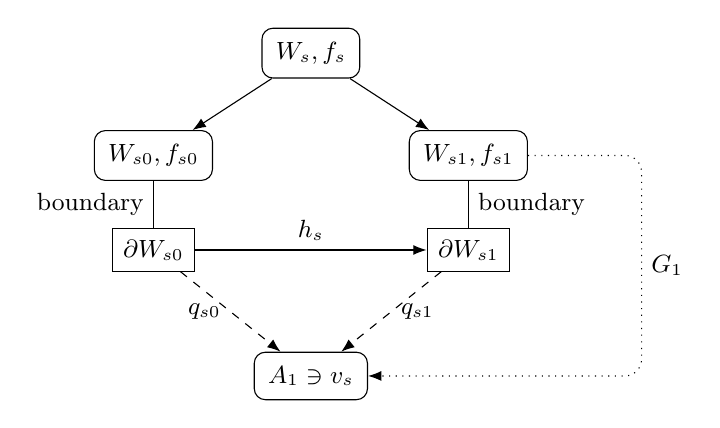
\begin{tikzpicture}[>=Latex, every node/.style={font=\small},
  world/.style={draw,rounded corners,inner sep=5pt},
  boundary/.style={draw,inner sep=4pt}]
 \node[world] (w) at (0,2.4) {$W_s,f_s$};
 \node[world] (w0) at (-2,1.1) {$W_{s0},f_{s0}$};
 \node[world] (w1) at (2,1.1) {$W_{s1},f_{s1}$};
 \node[boundary] (b0) at (-2,-.1) {$\partial W_{s0}$};
 \node[boundary] (b1) at (2,-.1) {$\partial W_{s1}$};
 \node[world] (a) at (0,-1.7) {$A_1\ni v_s$};
 \draw[->] (w) -- (w0);
 \draw[->] (w) -- (w1);
 \draw (w0) -- node[left] {boundary} (b0);
 \draw (w1) -- node[right] {boundary} (b1);
 \draw[->] (b0) -- node[above] {$h_s$} (b1);
 \draw[->,dashed] (b0) -- node[left] {$q_{s0}$} (a);
 \draw[->,dashed] (b1) -- node[right] {$q_{s1}$} (a);
 \draw[->,dotted,rounded corners=6pt] (w1.east) -- (4.2,1.1)
   -- node[right] {$G_1$} (4.2,-1.7) -- (a.east);
\end{tikzpicture}
\caption{A return-tree split. Solid arrows between worlds are
retained along their separate branches. Dashed boundary maps
persist in the common accumulator and agree on the test $v_s$.
Each dashed arrow denotes a compatible family of maps into the
proper projections of $A_1$.
The dotted full map is used to choose the plus boundary map
and need not be retained at later splits. Full maps of all
leaf worlds are installed only after the splitting tests have
been fixed.}
\label{iter:fig-return-tree}
\end{figure}

Process the nodes of each level successively. At a limit
height take the union of the worlds along each branch and
the union of the accumulators constructed so far. Their
sizes are still $\mu$. The boundary arrows into the union
accumulator exist by the chain and common-upper-bound clauses
in every proper projection. Full branch arrows and the
carried tuples also pass to the unions. This establishes
the invariant through height $\epsilon$.

At that height, apply lower-dimensional completion to each
leaf boundary map, successively enlarging the accumulator.
This supplies a full map of each $W_\eta$, for
$\eta\in{}^\epsilon2$, extending its retained boundary
map. There are fewer than $\mu$ leaves, so the final union
is still at level $\mu$. If two leaves first differ after
a node $s$, their images of $f$ have diagrams $\delta_0$
and $\delta_1$ over the common tuple $v_s$. Indeed the
corresponding copy of $v$ was in that child's boundary,
remained there along that branch, and its boundary image was never
changed except by composition with an accumulator arrow.
Thus the final images of $f$ occupy more than $\chi$
orbits over the entries of $(v_s:s\in{}^{<\epsilon}2)$.
This parameter list has size at most $\chi$. The orbit
bound of Lemma~\ref{calc:parameter-orbits} gives the
contradiction. The claimed equality of types of $v$ follows.

To pass from this type equality to the full pair diagrams, retain
an arbitrary bounded tuple $a$ from the lower face $X^-$.
The marginal of $b^+$ over
$X^+$ is the prescribed free lift from $e(X^-)$.
Relative isolation of the source type of $(b^-,v)$ and
Lemma~\ref{iso:free-isolation} therefore identify the actual type
of $(b^+,h(v))$ over $X^+$ with the free lift of that source type.

Choose sufficiently long bounded approximation lists in $X^-$
computing the source type.  Their images under $e$ compute its
free lift over $X^+$ by Theorem~\ref{calc:free-extension}.
Base homogeneity gives an isomorphism $X^-\cong X^+$ matching
$a$ and these lists with their images under $e$, since $e$
preserves their joint bounded diagram.  The transport assertion
for the approximation lists says that this isomorphism carries
the whole source type to the type of $(b^+,h(v))$.
Lemma~\ref{mark:pair-isomorphism} now extends it to an isomorphism
of the marked pairs matching $(a,v)$ with $(e(a),h(v))$.
Every bounded boundary list is of this form.  Thus its full
$\mathcal C_n$-diagram is preserved, including cross-face equalities.

We finish the induction by deriving completion from this
diagram equality. Present the source $J$ on a well-order.
Its boundary union is a natural collection of the
designated term sorts in that presentation. Choose nested
bounded lists $d_i$ exhausting $J$, including increasing
strong submodel enumerations in every vertex. We construct
extensions $K_i$ of $K$ and compatible assignments of
$d_i$ into $K_i$ satisfying
\[
 D_J(d_i,u)=D_{K_i}(d_i',h(u))
 \quad\text{for every bounded boundary list }u.
 \tag{C}
\]
Here and subsequently $h$ is composed with the current
extension arrow. At the start the assertion for the empty
list is exactly the boundary diagram equality just proved.

For the next list prescribe the source joint diagrams on
the parameter set consisting of the boundary images and
the previous assignment. Each bounded local request,
including the whole previous assigned list, is possible
by saturation: the parameter diagram agrees by $(\mathrm C)$.
This also checks repetitions and equalities between old
entries and boundary entries, so the requests define one
coherent prescription. Apply compact placement in a
well-ordered chart of $K_i$, keeping these previous
entries fixed. Work at one bounded cardinal large enough
for the profile count, the new tuple, and the testing
bound for the source boundary layout with the previous
tuple included. The resulting placement lies in a
level-$\mu$ extension $K_{i+1}$.

To check $(\mathrm C)$ beyond that initial testing cardinal,
pull the candidate diagrams back along $h$ to the natural
boundary layout of $J$. Their local possibility there
follows from the boundary diagram equality and saturation.
Lemma~\ref{calc:compact-placement} compactifies these
requests over this source layout, and
Proposition~\ref{calc:testing} says that agreement at the chosen
testing bound determines all bounded comparisons.
The actual images of the boundary inside $K_i$ have not
been assumed to form a natural layout. All uses of that
hypothesis are on the source layout after pullback.

Continue through $\omega$ steps and take the union of the
$K_i$. The working-package criterion, with the included
strong submodel enumerations, makes the union assignment
an arrow $J\to K^*$. Whenever a boundary entry is first
included in $d_i$, its equality test against that boundary
entry forces its assigned image to be $h$ of that entry.
The union arrow therefore extends the entire boundary
map. The map from $K$ is the chain inclusion. This proves
completion and closes the induction.
\end{proof}

\subsection{A bounded support for boundary tests}

We have extended boundary maps into common extensions.  Exact lifting
must instead land onto the given target.  The next lemma supplies bounded
data that control a tuple's boundary comparisons at a fixed bounded test
arity.  Together with uniform testing, this permits back-and-forth to
remain inside the two given systems.

\begin{lemma}[Fixed parameters for a boundary test function]
\label{iter:boundary-fixed-parameters}
Fix $n<\omega$. At further sufficiently closed levels,
let $J\in\mathcal C_n$, let $z$ be a bounded tuple of
$J$, and let $\sigma$ be a bounded infinite test arity.
There is a bounded list $a$ in $\partial J$ such that
every boundary automorphism $\alpha$ fixing $a$ pointwise
satisfies
\[
 D_J(z,u)=D_J(z,\alpha(u))
 \quad\text{for every boundary tuple }u
 \text{ of length at most }\sigma.
 \tag{F}
\]
A boundary automorphism means a compatible family of
isomorphisms of all proper projections; a full
automorphism of $J$ is not assumed.
\end{lemma}

\begin{proof}
The assertion is immediate for the empty boundary.
Suppose it fails otherwise. Choose a bounded infinite
$\chi$ with $\chi^{|z|+\aleph_0}=\chi$, bounding
$\sigma$ and the orbit-counting and label costs. Let
$\epsilon$ be the least cardinal with $2^\epsilon>\chi$.
Choose a smaller eligible level $\nu$ such that
\[
 |z|+\sigma+2^\chi<\nu<\mu,
\]
where $\mu$ is the level of $J$, with all required testing bounds
below $\nu$ and with
Theorem~\ref{iter:boundary-completion} available at $\nu$.
The further closure requirement on the level of $J$
ensures this choice. It is a finite refinement for this
fixed $n$.

Fix a well-ordered presentation $J=F_n(I)$. Construct
continuous subpresentations $J_i$ of size $\nu$ for
$i\le\epsilon$, beginning with $z$ in $J_0$.
At step $i$, the boundary of $J_i$ is a bounded parameter
set in $J$. By the assumed failure, a boundary
automorphism $\alpha_i$ of $J$ fixes it pointwise and
changes the value of the function at some tuple $u_i$
of length at most $\sigma$. Thus
\[
 D_J(z,u_i)\ne D_J(z,\alpha_i(u_i)).
 \tag{S}
\]
We choose $J_{i+1}$ containing both tests so that
$\alpha_i$ restricts to an automorphism of its boundary.

Here is the support closure for this choice. Begin with
the positions for $J_i$, $z$, $u_i$, and
$\alpha_i(u_i)$, padding to size $\nu$. For every element
of every proper projected subpresentation currently
generated, add positions for its image and its inverse
image under the corresponding face map of $\alpha_i$.
There are finitely many faces and $\nu$ elements in their
union, and each representation uses finitely many
positions. Repeat this operation countably many times.
The resulting position set still has size $\nu$.
Every element generated at its union appeared at a
finite stage, so both its image and inverse image are
generated in the union. Hence all restricted face maps
are onto and remain compatible with the specified
inclusions. They give the asserted boundary
automorphism of $J_{i+1}$. At a limit use the union of
the position sets. Mixed diagram preservation transfers
$(\mathrm S)$ to $J_{i+1}$, since $|z|+\sigma<\nu$.

Now build a binary tree of boundary embeddings
\[
 q_s:\partial J_i\longrightarrow\partial A,
 \qquad s\in{}^i2,
\]
where $A$ is an increasing accumulator of size $\nu$.
Start with $A=J_0$ and the identity map on $\partial J_0$.
At a successor node first apply completion to $q_s$
on $J_i$ and then amalgamate $J_{i+1}$ over that full
copy of $J_i$. This yields an arrow
$G_s:J_{i+1}\to A'$ whose boundary extends $q_s$.
Define the two next boundary embeddings by
\[
 q_{s0}=\partial G_s,
 \qquad
 q_{s1}=(\partial G_s)\alpha_i^{-1}.
\]
They restrict to the same old $q_s$, because
$\alpha_i$ fixes $\partial J_i$ pointwise. The common
parameter test $G_s(u_i)$ is the image of $u_i$ on
branch $s0$ and of $\alpha_i(u_i)$ on branch $s1$.
Only these boundary embeddings are retained for later
steps; the full map $G_s$ is temporary.

At limits the continuity of the $J_i$ and the
common-upper-bound clauses give the boundary maps into
the union accumulator. At height $\epsilon$, complete
the boundary maps to full maps of $J_\epsilon$, one
leaf at a time. The full maps at the leaves carry $z$.
If two leaves first separate at $s\in{}^i2$, their
images of $z$ have the two distinct diagrams from
$(\mathrm S)$ over the one retained test $G_s(u_i)$.
This follows from preservation by their final full maps
and from coherence of their boundary maps with the
chosen maps at the split.

There are at most $\chi$ nonterminal nodes, hence at
most $\chi$ parameters in all the splitting tests.
There are $2^\epsilon>\chi$ distinguishable leaf
images of $z$. All leaf completions and all unions
remain at level $\nu$, since $2^\chi<\nu$.
Lemma~\ref{calc:parameter-orbits} again contradicts
this number of orbits over the tests. Thus the bounded
fixing list $a$ exists.
\end{proof}

\begin{theorem}[Exact boundary lifting]
\label{iter:exact-boundary}
For each finite $n$, at further sufficiently closed
levels every boundary isomorphism
$h:\partial J\overset{\cong}{\longrightarrow}\partial K$
between $\mathcal C_n$-objects at the same level
extends to an isomorphism $J\cong K$ onto the given
target. All the prescribed marks and bounded named
data are preserved.
\end{theorem}

\begin{proof}
We build a back-and-forth sequence of matches
$a\mapsto a'$ of bounded tuples, maintaining
\[
 D_J(a,u)=D_K(a',h(u))
 \quad\text{for every bounded boundary tuple }u.
 \tag{BF}
\]
For the empty tuple this is
Lemma~\ref{iter:boundary-diagrams}. Suppose that a
match satisfying $(\mathrm{BF})$ has been chosen, and let $z$
be any bounded enlargement of $a$ in $J$.

Take a bounded infinite $\sigma$ at least the uniform
testing bound for a tuple of length $|z|$ over the
natural boundary layout of a $\mathcal C_n$-object.
Choose fixing data $c$ for $z,\sigma$ in $\partial J$
by Lemma~\ref{iter:boundary-fixed-parameters}.
The maintained equality with the particular boundary
list $c$ gives
\[
 D_J(a,c)=D_K(a',h(c)).
\]
Working-package homogeneity supplies a full
isomorphism $H:J\cong K$ carrying $a$ to $a'$ and
$c$ to $h(c)$. Put
$\alpha=(\partial H)^{-1}h$. This is a boundary
automorphism of $J$ fixing $c$ pointwise. Therefore,
for every boundary tuple $u$ of length at most
$\sigma$,
\[
 \begin{split}
 D_K(H(z),h(u))
 &=D_J(z,\alpha(u))\\
 &=D_J(z,u).
 \end{split}
 \tag{BT}
\]

We justify explicitly the passage from these tests
to all bounded boundary tests. By
Theorem~\ref{iter:boundary-completion}, embed $J$
into a same-level extension $K^*$ of $K$ by an arrow
$j$ extending $h$. Both $j(z)$ and $H(z)$ are now
tuples in $K^*$, and $(\mathrm{BT})$ says that their diagrams
agree over boundary tests from $K$ of size at most
$\sigma$. The boundary of $K$, in a well-ordered
chart of $K$, is a natural collection of term sorts.
The types of these two tuples over $K$ have order
placements by the one-dimensional calculus.
Proposition~\ref{calc:testing} restricted to this natural
boundary layout therefore gives equality over every
bounded boundary test. Preservation by $j$ then
shows
\[
 D_K(H(z),h(u))=D_J(z,u)
\]
for all bounded $u$. Thus $z\mapsto H(z)$ extends
the previous match and satisfies $(\mathrm{BF})$.

Apply this extension step alternately to $J,K$ with
$h$, and to $K,J$ with $h^{-1}$. Their level has
countable cofinality, so countably many bounded
enlargements can exhaust both systems. In each
vertex choose increasing smaller strong submodels
whose enumerations are included in these tuples.
The union assignment is onto in every component
and is an arrow by the working-package map
criterion; the reverse construction gives its
inverse arrow. If an entry lies on the boundary,
its equality test with that boundary entry in
$(\mathrm{BF})$ forces its image to be exactly the image
under $h$. The resulting isomorphism therefore
extends all of $h$, as required.
\end{proof}

\section{A minimal type and its geometry}
\label{geom:section-geometry}

We continue with the fixed AEC $\K$ that is categorical in unboundedly
many cardinals.  Throughout this Section, a level is eligible for the
single-model working scheme and for the refinements of the calculus
that are explicitly invoked.  The first level chosen below is denoted
by $\lambda_0$.  The level used for all finite marked constructions will
be a later cardinal $\lambda$; these two choices serve different purposes.

\begin{lemma}[Preservation of nonalgebraicity]
\label{geom:nonalgebraic}
Let $p$ be a nonalgebraic singleton type over an object $A$ of a working
scheme.  Its free lift over an extension $B$ is nonalgebraic.  The same
assertion holds for a mixed arrow whenever the input arity and the
testing bounds lie below the smaller level.
\end{lemma}

\begin{proof}
Suppose that the free lift were realized by $c\in B$.  Include equality
with $c$ among its tests.  To evaluate that test, the free-extension
construction moves $c$ into $A$, over enough of the chosen
approximations for $p$.  Its value is then the value of equality with an
element of $A$.  Every such equality has value false for $p$, whereas
equality with its alleged realization $c$ has value true.  This
contradicts the evaluation rule in Theorem~\ref{calc:free-extension}.
The mixed-level construction uses the same rule with the bounds taken
below the input level.
\end{proof}

\begin{proposition}[A minimal type]
\label{geom:minimal-type}
There is a sufficiently closed single-model level $\lambda_0$, a model
$M_0\in\K$ of size $\lambda_0$, and a nonalgebraic singleton type
$p_0$ over $M_0$ such that, over every $M_0\leq_\K A\in\K$ of size
$\lambda_0$, there is exactly one nonalgebraic extension of $p_0$.
This extension is its free lift.
\end{proposition}

\begin{proof}
Choose $\lambda_0$ with the single-model working package, the
stationary calculus, the all-dominated hull construction, and the
singleton type bound of Theorem~\ref{lev:amalgamation}(3).
Thus there are at most $\lambda_0$ singleton
types over a model of that size.  We may require at the outset strict
closure under all the fixed bounds used below for finite tuples and
their bounded tests.

There is a nonalgebraic singleton type at this level.  For example,
extend an order presentation by a fresh skeleton point.  That point is
outside the old model: if it were a labeled term on finitely many old
indices, adding a second distinct skeleton point with the same order
pattern over those indices would make both equal that term, contrary
to the distinctness of the skeleton.

Suppose that no nonalgebraic singleton type at this level is minimal in
the stated sense.  A nonalgebraic type always has a nonalgebraic free
extension by Lemma~\ref{geom:nonalgebraic}.  Consequently every such
type has two distinct nonalgebraic extensions over some model of size
$\lambda_0$.

Let $\epsilon$ be the least infinite cardinal with
$2^\epsilon>\lambda_0$.  Then $\epsilon\leq\lambda_0$ and
$2^{|i|}\leq\lambda_0$ for $i<\epsilon$.  Construct a continuous chain
$(A_i:i\leq\epsilon)$ of models of size $\lambda_0$ and types
$p_\eta$ over $A_i$, for $\eta\in{}^i2$, as follows.  At a successor
step, split every current $p_\eta$ over a model extending $A_i$.
There are at most $\lambda_0$ such models.  Successive amalgamation
over $A_i$, followed by unions, puts all of them into one next base
$A_{i+1}$ of size $\lambda_0$.  Freely extend each of the two split
types to that base.  Their restrictions to the splitting model are
different, so they remain different, and
Lemma~\ref{geom:nonalgebraic} keeps them nonalgebraic.

Along each branch retain a witness model and the same distinguished
realization.  The required successor map exists by amalgamation with
identification of realizations having the same type over the preceding
base.  At a limit take the unions of the common bases and, separately
on each branch, of its coherent witness models.  The realization is
outside every base stage, so it is outside the union base.  All these
unions have size $\lambda_0$ because the construction has length at
most $\lambda_0$.  At the final stage distinct branches have different
types over $A_\epsilon$, witnessed at their first splitting stage.
This gives more than $\lambda_0$ singleton types over $A_\epsilon$,
contrary to the type bound.  A minimal $p_0$ therefore exists.  Its
unique nonalgebraic extensions are free by existence of free lifts.
\end{proof}

The passage from a minimal type to closure and dimension follows the
geometric pattern of first-order categoricity developed through strongly
minimal sets; see Baldwin and Lachlan \cite[Sections~1--2]{BaldwinLachlan1971}.
Here the required containment, exchange, and change-of-base properties
are established directly for the AEC and its locally constructed types.

\subsection{Finite configurations over the chosen model}

\begin{definition}
\label{geom:points}
For $M_0\leq_\K M$ with $\|M\|\geq\lambda_0$, let $P(M)$ be the
set of realizations of $p_0$ in $M$.  More explicitly, $a\in P(M)$
means that in a strong section $N\leq_\K M$ of size $\lambda_0$
containing $M_0\cup\{a\}$, the type $\tp(a/M_0)$ is $p_0$.
A finite ordered list of distinct points in $P(M)$ is independent if
its type over $M_0$, computed in such a section, is the product of the
corresponding copies of $p_0$.
\end{definition}

These definitions do not depend on the section.  Two sections lie in
a third section of size $\lambda_0$, by the L\"owenheim--Skolem axiom
and coherence.  The embeddings into that section preserve their types
over $M_0$.  Products are permutation invariant, so independence is a
property of the underlying finite set.  Strong embeddings over $M_0$
preserve and reflect both membership in $P$ and finite independence.

We give a precise meaning to the containment test used in constructing
closure.  Fix a finite configuration $F\cup\{x\}\subseteq P(M)$ and
a size-$\lambda_0$ section $N$ containing it and $M_0$.  Say that $F$
\emph{forces} $x$ if, whenever $f:N\to W$ is a strong embedding fixing
$M_0$, with $W$ of size $\lambda_0$, and
$M_0\leq_\K D\leq_\K W$ has size $\lambda_0$ and contains $f[F]$,
one has $f(x)\in D$.  Thus the test permits a common extension of the
finite configuration and the proposed model; it does not presume that
intersections of strong models are strong models.

The test is invariant under the type of the entire finite
configuration over $M_0$.  Indeed, an identification of two copies of
that type is witnessed in an amalgam.  Any further configuration
witnessing failure of forced containment can be amalgamated with that
identification over the first witness model.  Its avoiding submodel
and the omitted point remain disjoint at that point because the maps
are injective.  This transports the failure to the second copy.  The
reverse transport is identical with the copies interchanged.

\begin{lemma}[The containment test]
\label{geom:containment-test}
For a finite independent set $S\subseteq P(M)$ and $x\in P(M)$,
$S$ fails to force $x$ if and only if $S\cup\{x\}$ is independent
with $x\notin S$.
\end{lemma}

\begin{proof}
First suppose that a coupling contains a model $D$ over $M_0$ and $S$
but omits $x$.  The type of $x$ over $D$ is a nonalgebraic extension of
$p_0$.  By Proposition~\ref{geom:minimal-type} it is the free lift of
$p_0$.  Restricting its parameters to $S$ shows, by
Proposition~\ref{calc:products}, that $x$ has product type with $S$ over
$M_0$.

Conversely suppose that $S,x$ has product type.  Use
Theorem~\ref{iso:all-lengths} to obtain a model all-dominated over
$M_0+S$, and amalgamate it with the actual finite configuration,
identifying the copy of $S$.  The domination conclusion of
Proposition~\ref{iso:prime} makes $x$ free over this model from $M_0$.
It is outside the model by Lemma~\ref{geom:nonalgebraic}.  The same
amalgamation can retain any further specified finite entries of the
original configuration.  This is a coupling witnessing that $S$ does
not force $x$.
\end{proof}

\begin{theorem}[The geometry of the minimal type]
\label{geom:pregeometry}
On $P(M)$, for every $M_0\leq_\K M$ of size at least $\lambda_0$,
the preceding finite independence is the independence relation of a
finitary pregeometry.  Its closure, denoted by $\cl_M$, has the
following properties.
\begin{enumerate}
\item For finite $F\subseteq P(M)$ and any maximal independent
      $S\subseteq F$, the set $\cl_M(F)$ consists exactly of those
      points that do not independently extend $S$.  Equivalently,
      $\cl_M(F)$ is the set of points forced by $F$.
\item Strong embeddings over $M_0$ preserve and reflect finite
      closure.  If $M_0\leq_\K A\leq_\K M$, then
      $P(A)$ is relatively closed in $P(M)$.
\item For finite $F$, $|\cl_M(F)|\leq\lambda_0$.  For every infinite
      $F\subseteq P(M)$,
      \[
      |\cl_M(F)|\leq |F|+\lambda_0.
      \]
\end{enumerate}
In particular bases exist, all bases have the same cardinality, and
each point of the span of a basis has finite basis support.
\end{theorem}

\begin{proof}
Choose a maximal independent subset $S$ of a finite $F$.  Every
$y\in F\setminus S$ fails to independently extend $S$, so
Lemma~\ref{geom:containment-test} says that every model containing $S$
in the actual configuration must contain all of $F$.  A point that
fails to independently extend $S$ is therefore forced by $F$.
If $x$ independently extends $S$, the avoiding dominated model from
Lemma~\ref{geom:containment-test} can be adjoined while retaining
$F,x$.  It contains $F$ by the preceding observation and omits $x$.
Thus $F$ does not force $x$.  This proves the first assertion and its
independence of the choice of $S$.

Define closure on arbitrary subsets by taking the union of closures
of finite subsets.  Extensivity and monotonicity hold directly from
the containment test.  To verify idempotence on finite configurations,
suppose that finitely many $y_j$ are in $\cl_M(F)$ and that $x$
independently extends a maximal independent $S\subseteq F$.  The
avoiding model over $S$ can be coupled with the whole finite
configuration $F,(y_j),x$.  It contains $F$ and every $y_j$, because
all these points are forced by $S$, and it omits $x$.  Hence the
$y_j$ cannot force $x$.  Finite character now yields idempotence for
all subsets.

For exchange, it suffices by finite character to take finite $F$ and
points $x,y$ with
\[
y\in\cl_M(F\cup\{x\})\setminus\cl_M(F).
\]
If $x\in\cl_M(F)$, idempotence would imply $y\in\cl_M(F)$, so
$x\notin\cl_M(F)$.  Let $S$ be a maximal independent subset of $F$.
Then $S,x$ and $S,y$ are independent.  Since every member of $F$ is
already forced by $S$, the set $S\cup\{x\}$ is maximal independent
in $F\cup\{x\}$.  The displayed membership says that $S,x,y$ is
dependent.  Permutation invariance of products makes $S,y,x$
dependent as well.  Applying the first assertion with $S\cup\{y\}$
gives $x\in\cl_M(F\cup\{y\})$.  This is exchange.

Preservation and reflection follow from the invariant finite-type
definition and the containment test.  For relative closedness, take
finite $F\subseteq P(A)$ and $x\in\cl_M(F)$.  Choose
$D\leq_\K A$ of size $\lambda_0$ containing $M_0\cup F$, and then
choose a section of $M$ containing $D\cup\{x\}$.  Forced containment
gives $x\in D\subseteq A$.  The finite closure of $F$ lies in this
same $D$, proving the finite cardinal bound.  There are $|F|$ finite
subsets of an infinite $F$, so finite character proves the displayed
bound.

For completeness, a maximal independent subset of a set can be
constructed by well-ordering it and retaining a point precisely when
it is outside the span of the points retained earlier.  Finite
character makes the resulting set independent, and maximality makes
it spanning.  If an independent set is spanned by a finite set of
$n$ points, it has at most $n$ points: successively insert its points
into a spanning list, using exchange to remove one of the original
points whenever a new independent point is inserted.  After $n$
insertions no further independent point is in the span.  This also
proves equality of finite basis sizes.

For infinite bases $H,J$ of the same closed set, choose for each
$j\in J$ a finite support $S_j\subseteq H$.  Then
$\cl(J)\subseteq\cl(\bigcup_{j\in J}S_j)$.  Independence of $H$
implies $H\subseteq\bigcup_{j\in J}S_j$, because a member of $H$
cannot belong to the span of the other members.  Hence
$|H|\leq|J|$; interchanging the bases gives the reverse inequality.
The finite argument excludes the possibility of one basis finite
and the other infinite.  Finally, for a closed $C$, the operator
$U\mapsto\cl(C\cup U)\setminus C$ on $P(M)\setminus C$ satisfies
the same closure and exchange axioms.  Finite character follows by
discarding all but the finitely many entries of $U$ in a dependence
witness.  Applying the preceding constructions to this operator
gives relative bases and their finite supports.
\end{proof}

\subsection{Pointed levels and change of base}

Choose an enumeration $\bar m_0$ of $M_0$ and place it as a strong
model in a sufficiently large well-ordered presentation of $\K$.
Such a placement exists by the order construction and categoricity at
$\lambda_0$.  Fix the stabilized diagram $\Delta$ of this entire
enumeration.  The initial supporting positions of this placement will
be held fixed in later order presentations.

\begin{proposition}[Pointed working levels]
\label{geom:pointed-levels}
At all sufficiently closed levels $\mu$ above the bounds for
$|\bar m_0|=\lambda_0$, models with a distinguished strong copy of
$M_0$ whose enumeration has diagram $\Delta$ form a categorical
working scheme.  Arrows preserve the indicated copy pointwise.
For a pointed model $B$ at such a level, $p_0$ has a unique
nonalgebraic extension $p^B$ over $B$; it is its free lift.  This family
lifts freely along pointed arrows, including the permitted mixed
arrows.  Naming further bounded data of a fixed diagram within the
base does not change type computation over the whole base.
\end{proposition}

\begin{proof}
The enumeration is a bounded tuple at $\mu$.  Bounded-diagram
homogeneity in Proposition~\ref{lev:closure-categoricity} carries it
between any two instances of $\Delta$ by an isomorphism of the entire
models.  The pointed version of the working package follows by
reserving its supporting positions and including the enumeration in
every relevant diagram, as in
Proposition~\ref{lev:named-package}.

Existence of $p^B$ is mixed free extension of $p_0$, and
Lemma~\ref{geom:nonalgebraic} gives nonalgebraicity.  To prove
uniqueness, take two nonalgebraic extensions over $B$.  A distinguishing
test for singleton types may be chosen with a fixed bound below
$\lambda_0$.  For any such parameter set $Z\subseteq B$, choose
$M_0\leq_\K A\leq_\K B$ of size $\lambda_0$ containing $Z$.
Both types restrict to nonalgebraic extensions of $p_0$ over $A$ and
are equal there by Proposition~\ref{geom:minimal-type}.  Their
diagrams on $Z$ are consequently equal.  The bounded testing theorem
gives equality over $B$.  Uniqueness and transitivity of free
extension prove the assertion for pointed arrows.

All distinguished data here already belong to the parameter model.
An amalgam over that model fixes them, and an identification of types
over that model respects them.  Thus adding them as constants does
not change this type computation.
\end{proof}

\begin{proposition}[Change of base for the geometry]
\label{geom:base-change}
Let $B$ be a pointed model at a sufficiently closed level much larger
than $\lambda_0$.  A finite list of points in an extension of $B$ is
independent over the closed set $P(B)$ in the geometry of
Theorem~\ref{geom:pregeometry} if and only if its type over $B$ is the
product of the corresponding copies of $p^B$.
\end{proposition}

\begin{proof}
A product can be witnessed by successive free realizations in models
containing all preceding entries.  Each realization is outside that
model by Lemma~\ref{geom:nonalgebraic}.  Its point set is relatively
closed, so the realization is outside the geometric span of $P(B)$
and the earlier entries.  This proves one implication.

For the converse let $x$ be a finite list independent over $P(B)$.
Fix a parameter test $Z\subseteq B$ large enough to be used in the
uniform comparison of the type of $x$ over $B$, but with
$|Z|<\lambda_0$.  Choose a regular infinite $\theta<\lambda_0$
with $|Z|<\theta$.  We may and do choose $\lambda_0$ closed enough
that the comparisons and local-character bounds used here fit below
it.

Inside $B$ choose lists $x_i$, $i<\theta$, so that every
$D^\K(x_i,Z)$ equals $D^\K(x,Z)$ and all the $x_i$ together are
independent over $M_0$.  To make the successor choice, include in the
bounded match the entire enumeration of $M_0$, $Z$, and all earlier
copies.  The original $x$, being independent over $P(B)$, is independent
from those earlier copies.  Saturation realizes its joint diagram
inside $B$.  Diagram equality is witnessed by an isomorphism, so it
preserves every finite independence comparison over $M_0$.  The total
parameters at every choice are bounded at the level of $B$.

Take a strong section $N\leq_\K B$ of size $\lambda_0$ containing
$M_0$, $Z$, and all the copies.  Their finite sublists have product
type over $M_0$.  The independent-list and finite-domination
conclusions of Theorem~\ref{iso:independent-lists} give a continuous
witness chain $(A_i:i\leq\theta)$ inside $N$, starting at $M_0$, in
which $x_i$ is free over $A_i$ from $M_0$ and is included in
$A_{i+1}$.  One may keep the chain inside $N$: at each step primeness
embeds the required all-dominated increment into $N$ over its already
placed base and the specified next list.  At limits finite domination
keeps the next finite list free, and unions remain strong in $N$.

Since $\cf(\theta)>|Z|$, local character applies to $\tp(Z/A_\theta)$.
It is free from some $A_i$.  For a later $j<\theta$, its restriction
to $A_{j+1}$ is free over $A_j$, so $Z$ and $x_j$ have product over
$A_j$.  The type of $x_j$ over $A_j$ is free from $M_0$.
The base-change identity in Proposition~\ref{calc:products} therefore
says that $x_j$ has product with $Z$ over $M_0$.  In particular
$D^\K(x_j,Z)$ is determined by $p_0$ and $\tp(Z/M_0)$.

A known product of the $p^B$ has this same joint diagram with $Z$:
products of free lifts are free lifts of products, and one may
restrict the resulting type to $M_0$ together with $Z$.  Since
$D^\K(x,Z)=D^\K(x_j,Z)$, the two candidate types over $B$ agree on
every test of the uniform comparison size.  Bounded testing makes
their full types equal.  This proves the converse.
\end{proof}

\subsection{Eliminating proper extensions with unchanged geometry}

The obstruction considered here is related to Vaughtian pairs: proper
extensions of the same cardinality with no new realizations of a fixed
nonalgebraic type; compare \cite{GrossbergVanDieren2006}, where the type
is based on a limit model.  Here finite marked systems and exact boundary
lifting eliminate the obstruction in the pointed setting.

The next use of the marked construction requires a type prescription
that can be chosen from a fixed set before choosing the common level.
We record the uniformity explicitly.

\begin{lemma}[Anchoring a singleton type]
\label{geom:anchored-type}
\label{geom:root-prescription}
There is a fixed cardinal $\beta$, depending on the single-model
template, its singleton comparison bound, and the fixed point, with
the following property.  If $A$ is a sufficiently closed pointed
model and $r$ is a nonalgebraic singleton type over $A$, a list
$c\subseteq A$ of length at most $\beta$ can be named so that:
\begin{enumerate}
\item the joint stabilized diagram of $c,\bar m_0$, together with a
      fixed majority prescription, defines a unique nonalgebraic
      singleton type $r^B$ over every sufficiently closed model $B$
      having that named diagram;
\item the prescription at $A$ is $r$, and the family $r^B$ lifts
      freely along arrows preserving the names, including across
      eligible levels;
\item the prescription occurs at arbitrarily large eligible
      single-model levels.
\end{enumerate}
The possible descriptors obtained this way form a set, with their
length bound independent of $\|A\|$.
\end{lemma}

\begin{proof}
Fix a sufficiently large uniform testing arity $\tau$ for singleton
types, including the bound needed to apply compact placement to those
tests.  The approximation construction for
Theorem~\ref{calc:free-extension} gives a list $c=(c_i:i<\beta')$ of
approximations in $A$ that computes $r$ by majority on all these
tests.  Its length and all ancillary approximation data can be bounded
by one cardinal $\beta$, independently of the level.  Choose the
length larger than the exception bound for the tests; increase
$\beta$ also to include the fixed point data.  The prescription is
the value attained by all but the permitted number of entries in
$D^\K(c_i,z)$, for each test $z$ of arity at most $\tau$.

Freely lift the actual $r$ to arbitrarily large eligible models
containing $A$.  Query matching over the fixed approximation list
shows that these lifts compute exactly the same majority
prescription.  They are nonalgebraic by
Lemma~\ref{geom:nonalgebraic}.  For another sufficiently closed
pointed $B$ with the same named diagram, embed $B$ into such a larger
instance, respecting the names.  This is possible by bounded-diagram
homogeneity and mixed placement.  Restrict the lifted type to that
copy of $B$.  It is nonalgebraic, since its realization is outside the
larger parameter model, and query matching makes its bounded answers
the prescribed ones.

Any two types having these answers are equal by the singleton
comparison bound.  Thus the construction is independent of the
larger instance and the chosen embedding.  A free lift along an arrow
preserving the names has the same prescribed answers: the
approximation evaluation is transported by matching each query over
the named list inside the old base.  Uniqueness therefore identifies
it with the prescribed receiving type.  At $A$ the answers are those
of $r$ by the choice of $c$.

The list lengths have a fixed set bound.  Their stabilized diagrams,
the fixed testing arity, and the majority rule range over a set of
descriptors.  Only descriptors realized at arbitrarily high eligible
single-model levels are needed; the preceding construction proves
that the descriptor extracted from an actual $r$ has this property.
The named diagram itself can be witnessed at one fixed eligible
level large enough for arity $\beta$, by saturation for diagrams from
larger levels.  Proposition~\ref{lev:named-package} therefore applies
with a lower threshold depending on $\beta$ and the original working
scheme, rather than on $\|A\|$.  In particular, extracting the names
from a model of size $\lambda$ does not require moving above
$\lambda$ in order to use the pointed working scheme at that level.
\end{proof}

\begin{theorem}[No proper pair with unchanged points at one level]
\label{geom:no-growth}
There is a sufficiently large cardinal $\lambda>\lambda_0$ such that
there is no proper strong inclusion $A<_\K B$ of pointed models of
size $\lambda$ with $P(A)=P(B)$.
\end{theorem}

\begin{proof}
Take the set of anchored descriptors from
Lemma~\ref{geom:anchored-type}.  Choose $\lambda$ at a common level
for all finite marked constructions for these descriptors, using
Theorem~\ref{close:common-levels}.  Require also all the relevant
single-model and pointed bounds, and $\lambda>\lambda_0+\beta$.
This is a choice uniform in the possible descriptor.  In particular
the choice does not depend on a pair that might later be assumed to
exist.

Suppose toward a contradiction that $A<_\K B$ is such a pair, and
choose $a\in B\setminus A$.  Apply
Lemma~\ref{geom:anchored-type} to $r=\tp(a/A)$ and name its list
$c$.  We work in the pointed scheme also naming this list, with its
fixed joint diagram.  Write $\mathcal C_n$ for its $n$-fold marked
iteration with the root prescription $r$, as in
Theorem~\ref{iter:finite-systems}.

Every one-step all-dominated increment of this scheme has no new
$P$-points.  Indeed, pointed categoricity carries its base, including
the named list $c$, onto $A$.  Transporting the witness $A<_\K B$
back gives an extension with a realization of the required $r$ and
unchanged $P$.  Primeness embeds the all-dominated increment into
that extension over its base and mark.  Since strong maps preserve
and reflect $P$ and fix the base, the increment has exactly the base
points.

It follows by induction that the $P$-points in the top of every
$\mathcal C_n$ object are precisely those in its root.  For the
induction step, its lower and upper layers are $\mathcal C_{n-1}$
objects and hence each has the points of its own root.  Projection
onto the new axis is a valid one-step marked increment by
Theorem~\ref{iter:finite-systems}.  The two roots therefore have the
same points, proving the assertion for the entire object.

We next construct coherent finite systems.  For each $n<\omega$
choose an object $J_n\in\mathcal C_n$.  For every
$s\subseteq\{1,\dots,n\}$ choose an isomorphism
\[
e_{n,s}:J_{|s|}\longrightarrow P_sJ_n
\]
such that these maps commute with all further face projections, using
the increasing identifications of finite index sets.  Here the full
face map is the identity.  To make these choices, induct first on
$n$ and then on the size of a proper subset $s$.  For a proper subset
$u$ of the axes of $J_{|s|}$, let $t$ be the corresponding subset of
$s$.  The boundary map for $e_{n,s}$ on this face is
$e_{n,t}e_{|s|,u}^{-1}$, with the indicated index identifications.
The already chosen maps make these boundary prescriptions compatible.
Theorem~\ref{iter:exact-boundary} extends them to the desired
isomorphism.  At dimension zero it is simply pointed categoricity.
This constructs every $e_{n,s}$ with the asserted commutation.

For the finite subsets $s$ of any ordinal $I$, take a tagged copy of
the top vertex of $J_{|s|}$.  If $s\subseteq t$, use the top component
of $e_{|t|,u}$ followed by the inclusion of that face into the top,
where $u$ records the positions of $s$ in the increasing list of $t$.
The preceding commutation gives a directed system of strong maps.
All its roots are copies of the same actual $J_0$, and no vertex has
more $P$-points than that root.

The marks corresponding to different indices of $I$ are distinct in
this directed system.  It suffices to inspect a two-axis object.  Its
new mark lies in the root of its upper one-axis layer, whereas the
old mark is the nonalgebraic mark of that layer and is outside its
root.  Face isomorphisms preserve the marks, so the distinction
persists under all transition maps.

Take $I$ of cardinality $\mu>\lambda$, where $\mu$ is a sufficiently
closed single-model pointed level.  The ordinary directed colimit in
the AEC exists: a coherent diagram of injective maps is realized as
a diagram of inclusions in its direct limit, and the directed-union
axioms apply.  There are $\mu$ finite subsets of $I$, each contributing
at most $\lambda$ elements, and there are $\mu$ distinct marks.  Thus
the colimit $N$ has size exactly $\mu$.  Every element of $N$ comes
from one finite vertex.  Preservation and reflection of $P$ give
\[
P(N)=P(J_0),\qquad |P(N)|\leq\lambda.
\]
The enumeration of its distinguished $M_0$ retains the fixed
stabilized diagram $\Delta$ under the strong colimit embeddings.

On the other hand, there is a pointed model of size $\mu$ with more
than $\lambda$ points.  Start with any pointed model of that size.
Successively realize a nonalgebraic free extension of $p_0$ outside
the current model, for $\lambda^+$ steps.  The receiving models and
their unions may all be kept of size $\mu$.  The new realizations
are distinct and belong to $P$, so the union has at least
$\lambda^+$ points.  Pointed categoricity at $\mu$ would make this
model isomorphic to $N$ over $M_0$, a contradiction.

Only the stationary prescription $r$ was lifted to higher levels.
The assumed witness with unchanged $P$ was used solely at
$\lambda$.  The large colimit used the full AEC directed-union
axioms, rather than a same-level closure assertion for a marked
scheme.
\end{proof}

\begin{corollary}[No-growth and rank on the entire tail]
\label{geom:tail-no-growth}
Increase the threshold $\lambda$ if necessary to include the bounds
for the fixed point diagram.  In arbitrary cardinalities, if
$A\leq_\K B$ are pointed models with $\|A\|\geq\lambda$ and
$P(A)=P(B)$, then $A=B$.
Moreover, for every pointed model $M$ with $\|M\|>\lambda$,
\[
|P(M)|=\rk(P(M))=\|M\|.
\]
The point sets of strong submodels are relatively closed, and
relative bases and finite basis supports are available as in
Theorem~\ref{geom:pregeometry}; no eligibility condition is imposed
on these arbitrary cardinalities.
\end{corollary}

\begin{proof}
Suppose that $a\in B\setminus A$ and $P(A)=P(B)$.  Construct
increasing strong submodels $A_i\leq_\K A$ and $B_i\leq_\K B$ of
size $\lambda$, for $i<\omega$, all containing the distinguished
copy of $M_0$, so that
\[
A_i\leq_\K B_i,\qquad a\in B_i,\qquad
P(B_i)\subseteq A_{i+1}.
\]
For the successor choice, $P(B_i)$ has size at most $\lambda$ and
is contained in $A$, so the L\"owenheim--Skolem axiom places it,
together with $A_i$, in the next $A_{i+1}$.  Choose $B_{i+1}$ to
contain $A_{i+1}\cup B_i\cup\{a\}$.  Coherence makes all the
required inclusions strong.  The two unions $A_\omega\leq_\K
B_\omega$ have size $\lambda$.  The point diagram restricts
correctly to them, and
\[
P(B_\omega)=\bigcup_{i<\omega}P(B_i)
             \subseteq A_\omega.
\]
Thus their point sets are equal, while $a\in B_\omega\setminus
A_\omega$.  This contradicts Theorem~\ref{geom:no-growth}.

Now let $\|M\|=\kappa>\lambda$.  If $|P(M)|<\kappa$, choose a
strong submodel containing $M_0\cup P(M)$ of size at most
$|P(M)|+\lambda_0$.  Enlarge it inside $M$, if necessary, to a
strong submodel of size at least $\lambda$ and still less than
$\kappa$.  It has the same $P$ as $M$, contrary to the assertion
just proved.  Hence $|P(M)|=\kappa$.  If $H$ is a basis of $P(M)$,
the closure bound gives
\[
\kappa=|P(M)|=|\cl_M(H)|\leq |H|+\lambda_0.
\]
Since $\kappa>\lambda\geq\lambda_0$, it follows that
$|H|=\kappa$.  The final assertions were established in
Theorem~\ref{geom:pregeometry} independently of eligibility.
\end{proof}

\section{Geometric systems and classification by bases}
\label{sys:section-geometric-systems}

Throughout this section the distinguished model $M_0$, its fixed pointed
pattern, and the pregeometry $P$ are those of
Proposition~\ref{geom:pointed-levels} and
Theorem~\ref{geom:pregeometry}.
All model sizes exceed the threshold of
Corollary~\ref{geom:tail-no-growth}.  Thus a strong inclusion of pointed
models with equal $P$-sets is equality.  At an eligible uniform level
$\mu$, all vertices have size $\mu$.  A statement about unions of
objects at that level concerns chains whose total size is $\mu$, as in
the working conditions of Definition~\ref{lev:working-package}.

We first prove structural and presentation assertions without assuming
categoricity of systems.  The classification argument then proceeds by
the number of axes.  Its first assertion extends a root isomorphism and
prescribed bijections of the other basis pieces; this gives categoricity
for the current shape.  That categoricity supplies the working package
used to prove the second assertion: prescribed bijections of the basis
pieces added to a fixed system extend to an isomorphism over that system.
By splitting off the last axis, the second assertion gives the first at
the next dimension.  We establish the conditional package before carrying
out this paired induction.

\subsection{Shapes, relative bases, and arrows}

\begin{definition}[Admissible shapes and geometric systems]
\label{sys:shapes}
Let $A$ be a finite linearly ordered set of axes.  An admissible family
$L\subseteq\mathcal P(A)$ of \emph{active labels} is defined recursively.
On no axes the family is $\{\varnothing\}$.  If $k$ is a new last axis,
choose an upward closed subset $Q$ of the previously constructed family
$L$, and put
\[
 L'=L\cup\{s\cup\{k\}:s\in Q\}.
\]
Here upward closed means that $s\in Q$, $s\subseteq t$, and $t\in L$
imply $t\in Q$.

A geometric system of shape $L$ is a family
$(X_t:t\subseteq A)$ of pointed models in a common top model, with
$X_t\leq_\K X_u$ when $t\subseteq u$, satisfying the following condition.
There is a partition $(H_s:s\in L)$ of a basis of $P(X_A)$ such that
$H_s\subseteq P(X_s)$ and
\begin{equation}
\label{sys:vertex-span}
 P(X_t)=\cl_{P(X_A)}\left(\bigcup_{s\in L,\ s\subseteq t}H_s\right)
 \qquad(t\subseteq A).
\end{equation}
At uniform level $\mu$ we require $|H_s|=\mu$ for every $s\in L$.
The resulting scheme is denoted $\mathcal G_L$.
The basis partition witnesses the definition; it is not named in the
system structure.

For a vertex $t$, write
\[
 D_t(X)=\cl_{P(X_A)}\left(\bigcup_{r\subsetneq t}P(X_r)\right).
\]
For $t=\varnothing$ this is the closure of the empty set in the
pregeometry.  An arrow $X\to Y$ is a commuting family of pointed strong
embeddings for which a witnessing partition for $X$ extends to a
witnessing partition for $Y$.  Equivalently, after identifying $X$ with
its image, each finite tuple from $P(X_t)$ independent over $D_t(X)$
remains independent over $D_t(Y)$.
\end{definition}

The equivalence in the last sentence, including its independence from
the initially chosen partition, will be proved below.  All closures and
independence assertions are computed in a common containing pointed
model.  Theorem~\ref{geom:pregeometry} makes this convention
independent of the chosen common strong extension.
The notation $\cl_{P(X_A)}$ means the closure $\cl_{X_A}$ defined
there; its subscript emphasizes the pregeometry in which it is
computed.  We omit that subscript when the ambient model is clear.

\begin{lemma}[Combinatorics of shapes]
\label{sys:shape-combinatorics}
An admissible family contains $\varnothing$ and is closed under unions.
Its restriction to any subset of the axes is admissible, with the
inherited order.  Consequently every $t\subseteq A$ has a largest
active subset
\[
 a_L(t)=\bigcup\{s\in L:s\subseteq t\}.
\]
In a geometric system, $X_t=X_{a_L(t)}$ whenever $t$ is inactive.
\end{lemma}

\begin{proof}
The union assertion follows by induction on the axes.  Unions of old
labels are old.  If a union involves $s\cup\{k\}$ with $s\in Q$, its
old part is an active label containing $s$, and therefore belongs to
$Q$.  This also handles the union of two labels containing $k$.
Restriction to a set of axes replaces $L$ and $Q$, at every retained
step, by their restrictions.  The restricted $Q$ is upward closed in
the restricted $L$.  Steps on discarded axes make no contribution.
This proves the restriction assertion.

The displayed union is an active label, since the family is finite and
contains $\varnothing$.  The collections of active labels below $t$
and below $a_L(t)$ agree.  Equation~\eqref{sys:vertex-span} therefore
gives equality of their $P$-sets.  The inclusion
$X_{a_L(t)}\leq_\K X_t$ and
Corollary~\ref{geom:tail-no-growth} give equality of the models.
\end{proof}

\begin{remark}
Union closure alone would not imply the recursive last-axis
description.  For example, $\{\varnothing,\{1,2\}\}$ is union closed,
but its two layers on splitting off axis $2$ have different active
families.  We use the recursive definition, including the upward
closed set $Q$, when identifying a system with an arrow between
systems on fewer axes.
\end{remark}

\begin{lemma}[Replacement and extension of relative bases]
\label{sys:relative-bases}
Suppose $X$ is a geometric system.  For each active $s$, choose any
basis $B_s$ of $P(X_s)$ over $D_s(X)$.  Then the $B_s$ form a
witnessing partition for $X$.

A componentwise strong system embedding is an arrow precisely when
it preserves the relative independence in
Definition~\ref{sys:shapes}.  For an arrow, every witnessing partition
of its domain extends to one of its codomain.
\end{lemma}

\begin{proof}
Fix a witnessing partition $(H_s:s\in L)$, and enumerate $L$ in an
order extending inclusion.  For active $s$,
\[
 D_s(X)=\cl\left(\bigcup_{u\in L,\ u\subsetneq s}H_u\right).
\]
When the piece at $s$ is replaced, previously processed labels not
below $s$ are independent, together with the original piece at $s$,
over this lower span: they are parts of a single independent set.
Replacing $H_s$ by any basis of the same flat over its lower span
preserves both independence and the span of the union.  Explicitly,
let $C$ be the current pieces below $s$.  Then
$\cl(C\cup B_s)=\cl(C\cup H_s)=P(X_s)$, and $C\cup B_s$ is
independent.  The remaining current pieces were independent over
$\cl(C\cup H_s)$, since the full current partition was independent.
They remain independent over the equal flat $\cl(C\cup B_s)$.
Thus the new full partition is independent and has the same span.
Applying this replacement at the finitely many active labels gives the
first assertion and Equation~\eqref{sys:vertex-span} for the new
partition.

If pieces extend along an embedding, any finite independence
calculation in a vertex over its lower span is the same calculation
using the corresponding pieces in the larger independent set.
Relative independence is therefore preserved.

Conversely, let $(B_s)$ be an arbitrary witnessing partition of the
domain, viewed as a subsystem of $Y$.  Preservation implies that
$B_s$ is independent over $D_s(Y)$.  Extend it to a relative basis
$B_s\cup C_s$ of $P(Y_s)$ over $D_s(Y)$.  The first assertion, applied
to $Y$, says that these choices assemble into a witnessing partition
of $Y$.  This proves both the equivalence and the final assertion.
\end{proof}

\begin{lemma}[Structural properties and the last-axis description]
\label{sys:structural}
Arrows compose and satisfy coherence.  Same-level chains of total
size the level have unions in $\mathcal G_L$, with the common-upper-
bound clause also for arrows into a larger eligible level.

Restriction to any subset of axes preserves systems and arrows.
If $L'=L\cup\{s\cup\{k\}:s\in Q\}$, splitting off the last axis
identifies a system of shape $L'$ with an arrow $X\to Y$ in
$\mathcal G_L$ such that the complementary piece at $s$ has size
$\mu$ for $s\in Q$ and is empty for $s\notin Q$.
\end{lemma}

\begin{proof}
Composition follows from the relative independence criterion.
For coherence, suppose $X\subseteq Y$, and both embed by arrows in
$Z$.  Independence over $D_t(X)$ implies independence over $D_t(Z)$,
and hence over its subset $D_t(Y)$.  Componentwise coherence is the
AEC coherence axiom.

For a continuous chain, extend witnessing pieces successively using
Lemma~\ref{sys:relative-bases}, and take their unions at limit stages.
Every finite independent sublist and every finite dependence witness
occurs at a stage.  The resulting union pieces are independent and
span every vertex of the componentwise union.  Each contains $\mu$
elements from the first stage and has size at most $\mu$, so all
pieces still have size $\mu$.  For a chain which is not initially
continuous, insert its earlier unions: the preceding construction
applies recursively, and the common-upper-bound argument in the next
paragraph supplies its connecting arrows.

If each stage maps by an arrow into $Z$, a finite tuple independent
over the lower span of the union is independent over the lower span
at any stage containing it.  Its image is independent over $D_t(Z)$.
The componentwise AEC common-upper-bound axiom supplies the strong
maps, so the union map is an arrow.  This argument also permits a
larger level for $Z$.

On restricting to axes $B\subseteq A$, retain the pieces whose labels
are contained in $B$.  They are a basis of $P(X_B)$ and satisfy the
required span identities.  For a retained vertex all its proper
subsets are still retained; its relative independence test is
therefore exactly the old test.

Finally let $Z$ have shape $L'$, and put $X_s=Z_s$ and
$Y_s=Z_{s\cup\{k\}}$.  A partition for $Y$ is obtained by combining
$H_s$ with $H_{s\cup\{k\}}$ when $s\in Q$, and using $H_s$ alone
otherwise.  These choices extend the pieces of $X$, and their
complements have the asserted sizes.  Conversely, extend pieces of
$X$ to pieces of $Y$ along such an arrow, give the old pieces labels
$s$ and their complements labels $s\cup\{k\}$, and use $X$ and $Y$
as the two layers.  The span identities give a system of shape $L'$.
Inactive vertices cause no exception, by
Lemma~\ref{sys:shape-combinatorics}.
\end{proof}

For later use, preservation of relative independence also preserves
finite rank calculations modulo the lower span.  For finite tuples
$a,c$ in a vertex, the condition that $a$ be independent over
$D_t(X)\cup c$ is determined by the ranks, modulo $D_t(X)$, of
sublists of $a,c$.  These ranks are determined by which sublists are
independent.  Thus arrows preserve this condition as well.

\subsection{Order presentations and their rank}

\begin{proposition}[Tiled presentations]
\label{sys:tiling}
Let $L$ be admissible and let $\mu$ be sufficiently large for the
pointed pregeometry and the no-proper-pair conclusion.  The order
template $E$ gives a presentation in $\mathcal G_L$ as follows.
Choose a fixed initial order carrying the whole enumeration of $M_0$.
For each active label $t$, choose a tile $T_t$, preceded by a buffer
$B_t$, and concatenate these finitely many pairs after the initial
order, in any fixed order.  Every tile and buffer is a dense linear
order without endpoints of size $\mu$.  In vertex $s$ retain the
initial order, all buffers, and just the tiles with labels $t\subseteq
s$.

These presentations have the following properties.
\begin{enumerate}
\item Each active relative piece has rank $\mu$.
\item Order embeddings of the corresponding tiles and buffers,
fixing the initial pointed data, induce arrows, including between
different eligible levels.
\item A presentation has an extension by an arrow gaining $\mu$
independent complementary coordinates at every active label
simultaneously.
\item Tiles may be chosen with $\mu$ pairwise disjoint convex
substrips, each of size $\mu$.  Further insertions of such substrips
preserve the preceding assertions and the naturalness of the
underlying $\K$-diagrams.
\end{enumerate}
No categoricity assumption about $\mathcal G_L$ is used here.
\end{proposition}

\begin{proof}
Let $I_s$ be the indicated suborder and set $X_s=E(I_s)$, using the
literal embeddings supplied by Theorem~\ref{found:order-template}.
All $I_s$ have size $\mu$, since they contain all buffers.  The
models have size $\mu$ and are strongly included according to their
labels.  The initial order was chosen to contain the supports of the
fixed enumeration of $M_0$.  Its unchanged term pattern carries the
same pointed model in every vertex, and coherence gives the required
strong inclusion of $M_0$.

Choose a relative basis $H_s$ of $P(X_s)$ over the union of its
proper lower $P$-sets for every active $s$.  We first prove that the
indexed family of these choices is independent; this also proves
that the pieces are disjoint.  Suppose there is a finite circuit
of labeled entries, allowing a two-entry equality dependence when
two differently labeled entries coincide.  Choose a maximal label $s$ represented among its
entries.  Retain the finite term supports of all entries with label
$s$, and indeed retain every support position in a tile available
at $s$.  In each unavailable tile replace all support positions by
distinct positions in its preceding buffer, beyond all the finitely
many retained positions in that buffer.  Such positions exist because
the buffer has no greatest point and is dense.  No retained position
lies in that unavailable tile.  Consequently this replacement
preserves the order and equality pattern of all circuit supports and
fixes the whole initial pointed order.

The labels and this order pattern preserve the pointed finite
geometry comparisons.  One can formulate this either using the
natural $\K$-diagrams or by taking the term model on the fixed initial
order and the finite supports and applying its two pointed strong
embeddings into the original presentation.  In the latter formulation
Theorem~\ref{geom:pregeometry} preserves and reflects the
independence relation.

An entry with label $t\ne s$ in the circuit has no label properly
containing $s$, by maximality.  Thus $s\nsubseteq t$.  After the
replacement its term uses only common buffers, initial data, and
tiles with labels contained in $s\cap t$.  Its image belongs to
$P(X_{s\cap t})\subseteq D_s(X)$.  The entries with label $s$ have
not moved.  The preserved circuit makes a sublist of $H_s$ dependent
over $D_s(X)$, a contradiction.  The union is therefore independent.
It spans every vertex by induction on the labels: its relative basis
spans that vertex over lower vertices, which have already been
spanned.  If a vertex is inactive, the order retained there is exactly
the order retained at its largest active subset.  This proves the
decomposition without first assuming the system axioms.

We give the fresh-skeleton observation needed for the rank assertion.
If $J\subseteq I$ and $i\in I\setminus J$, the skeleton entry at $i$
does not belong to $E(J)$.  Otherwise it equals a labeled term on a
finite tuple of positions from $J$.  Enlarge the order by a second
position $i'$ having the same order pattern as $i$ relative to that
finite tuple.  Literal pattern preservation would make both
distinguished skeleton entries equal to that term.  This contradicts
their required distinctness.  The enlargement need only duplicate
the cut relative to the finite tuple, not the cut relative to all of
$J$.

For an active $t$, omit $T_t$ from $I_t$.  The resulting order still
has size $\mu$, contains the pointed data and all proper lower
vertices, and presents a strong submodel.  Enumerate $\mu$ points of
$T_t$ and adjoin them one at a time.  The fresh-skeleton observation
makes each successor inclusion proper.  All these models have size
$\mu$, because the buffers were retained.  By
Corollary~\ref{geom:tail-no-growth}, each successor adds a point of
$P$.  Choose one such point at each successor.  Relative closedness
of $P$ in strong submodels makes these choices independent over the
initial omitted-tile model.  There are $\mu$ choices, so the rank over
the proper lower vertices is at least $\mu$.  It is at most $\mu$
by the size of $X_t$.  This proves the first assertion, including the
root case $t=\varnothing$.

Next consider componentwise order embeddings into enlarged tiles and
buffers, identifying the source with its image.  Suppose a finite
tuple $a$ in $P(X_s)$, independent over $D_s(X)$, becomes dependent
over $D_s(Y)$.  Dependence has a finite witness consisting of points
from proper lower vertices of $Y$.  Fix the finitely many old
positions supporting $a$.  Move every other position needed for the
witness into its corresponding old tile or buffer, preserving its
order relative to the fixed positions.  Density and absence of
endpoints of the old order suffice for each finite pattern; it is
not necessary that the old order be dense in the enlarged order.
The initial pointed order remains fixed.  Each witness remains in
its designated proper lower vertex, now in $X$, and its finite
dependence diagram is preserved.  This contradicts independence of
$a$ over $D_s(X)$.  Lemma~\ref{sys:relative-bases} therefore gives an
arrow.  The proof did not require equal source and target sizes.

To obtain simultaneous gains, enlarge all tiles with $\mu$ fresh
points and, if desired, enlarge the buffers.  For a particular active
$t$, begin the strict-growth argument over the order containing the
old $t$-tile, all enlarged proper-lower tiles, all enlarged buffers,
and the initial data.  This base contains $X_t$ and all proper lower
vertices of $Y$.  Adjoining the fresh points of the $t$-tile yields
$\mu$ independent points over that larger base.  Hence the
complementary rank at $t$ is $\mu$.  The preceding arrow assertion
allows any old pieces to extend, and
Lemma~\ref{sys:relative-bases} combines the relative choices into
one partition.  This proves the simultaneous assertion.

Finally a lexicographic sum, indexed by a linear order of size
$\mu$, of dense endpoint-free orders of size $\mu$ is still dense
and endpoint-free and has size $\mu$.  Its summands are the desired
convex substrips.  In particular, for a presentation indexed by a
well-order $H$, one can use $H\times\Q$ and reserve intervals of
$H$ of order type and cardinality $\mu$.  Taking $H$ of order type
$\mu\cdot\mu$ supplies $\mu$ disjoint such intervals.  Additional
summands or strips do not change any of the preceding arguments.
Underlying $\K$-diagrams remain natural because the entire system
was obtained by designated term subcollections of the single
template $E$.
\end{proof}

\subsection{Obtaining the working package from categoricity}

\begin{proposition}[Conditional working package]
\label{sys:working-package}
Fix an admissible shape $L$.  Suppose that $\mathcal G_L$ is
categorical at every level in an unbounded class of eligible levels
closed sufficiently for the preceding constructions.  Assume also
the eligible-subclass hypothesis of Convention~\ref{lev:eligible-subclass}.
On an unbounded further class of sufficiently closed levels, it satisfies the full working
package of Definition~\ref{lev:working-package}, with its actual
system isomorphisms and its arrows from Definition~\ref{sys:shapes}.
The resulting diagrams, saturation, and calculus include mixed
arrows between eligible levels, and the output class retains the
eligible-subclass hypothesis.

The closure requirements are uniform in the finite shape and the
fixed pointed template.  They use only the smaller and larger input
levels specified by the general working-package construction.
\end{proposition}

\begin{proof}
The structural conditions are Lemma~\ref{sys:structural}.
Proposition~\ref{sys:tiling} supplies term presentations and mixed
presentation arrows before categoricity.  By the assumed
categoricity, every object at an input level is isomorphic to its
presentation.

We check the extra relative-basis condition throughout the reversal
argument.  In each tile and buffer use the order $H(\delta)$ from
Theorem~\ref{found:order-orbits}.  For a tuple of length $\theta$, record
its term labels, the fixed initial positions it uses, and, separately
in each of the finitely many variable orders, the order and
realized-cut record of its support positions.  If
$\theta<\cf(\delta)$, equal records are carried to one another by
order automorphisms of the respective tiles and buffers.  Their
product fixes the initial data and induces an automorphism of the
whole system.  The set of possible records has a bound depending
only on $\theta$, the finite shape, and the template.  Hence the
system orbits at that arity have a uniform set bound.

Number these orbits and record the arrows between them, together
with the partial map from support records to orbit names.  This is
again a bounded palette.  If reversal fails unboundedly often,
choose repeated profiles at eligible levels $a<\mu$ exactly as in
Theorem~\ref{found:reversal}, with $a^\theta\leq\mu$ and the required
large cofinalities for the orders.  Apply the ordinal-position
shrinking of Proposition~\ref{found:alignment} simultaneously to the
finitely many tiles and buffers.  Given at most $a$ parameters in
the large system, the resulting small presentation contains them,
has size $a$ in every tile and buffer, and computes the support
records of all its $\theta$-tuples correctly.  Its inclusion is an
actual arrow by Proposition~\ref{sys:tiling}.  Thus it is an aligned
small geometric system, not merely a componentwise subsystem.

For completeness, the contradiction uses two orbit names $p,r$ with
$p\to r$ and $r\not\to p$.  Repeatedly choose aligned small copies,
each containing the previous one, and process their at most
$a^\theta$ tuples in the large level.  Whenever a tuple can still be
sent to $p$, send it onward to $r$.  From that point it cannot reach
$p$.  Coherence makes the successive small copies a chain of
arrows.  After $\theta^+$ rounds every $\theta$-tuple of their union
occurred at a proper round.  Both unions exist by
Lemma~\ref{sys:structural}: the small union has total size $a$, and
the large construction has total size $\mu$.  Alignment says that
none of the tuples of the small union can reach $p$.  Categoricity
of that union at $a$ says that its orbit $p$ is realized, a
contradiction.  This proves eventual reversal at each fixed arity.

Mixed L\"owenheim--Skolem closure also has the required form.
In a presentation, close the supports of a prescribed small set
under finitely many intermediate and exterior positions in every
tile and buffer, repeat countably many times, and pad each order
to the chosen smaller eligible size.  The resulting dense
endpoint-free suborders give a small presentation containing the
set.  The initial pointed order is retained in full.  Its inclusion
is an arrow by Proposition~\ref{sys:tiling}.  Transport through a
presentation of an arbitrary large object gives mixed containment;
coherence supplies comparisons between such subobjects.

We now apply the first route of
Proposition~\ref{lev:scheme-diagram-routes}.  Its structural
hypothesis is Lemma~\ref{sys:structural}; its presentation and mixed
downward-closure hypotheses are Proposition~\ref{sys:tiling} and
the preceding paragraph.  Categoricity is the input assumption,
and the required arity-by-arity reversal and uniform orbit bounds
were proved above.  Thus the proposition applies to the actual
system arrows, including their relative-basis condition.

In particular, the canonical comparison at a smaller input level
is computed in a small geometric subobject.  Two such sections
are contained in a common small section by mixed downward closure,
and coherence gives its arrows, so the comparison is well defined.
The projections between comparisons at two input levels are onto
because the smaller system is a tiled presentation and extends by
the mixed order arrows of Proposition~\ref{sys:tiling}.  The bounded
palette therefore stabilizes, exactly as in the first route of
Proposition~\ref{lev:scheme-diagram-routes}.

Choose receiving levels which remain eligible, are strictly closed
under the resulting arity bounds, and have sufficiently large
smaller input levels below them for every bounded request.
These are the closure refinements described in
Section~\ref{lev:refining-levels}, supplied simultaneously in
Theorem~\ref{close:common-levels}; closure under the next input
level is not being used to infer eligibility by itself.  At such a
level, countable alternating matching in smaller input-level
sections gives actual system isomorphisms on equal bounded
diagrams, and realizes possible bounded joint diagrams over their
given subtuples.  Thus diagrams, homogeneity, and saturation have
the system interpretation required here, rather than merely their
componentwise $\K$ interpretation.  Order embeddings and order
amalgamation make the diagrams natural on term tuples, so
Proposition~\ref{lev:diagram-coding} also applies.

It remains to check the additional exhaustion condition, which
Proposition~\ref{lev:scheme-diagram-routes} explicitly leaves as a
separate obligation.  A finite tuple independent modulo the
proper lower vertices stays so when its target diagram agrees with
a tuple placed along an actual presentation arrow: the comparison
is realized by a system isomorphism, and such an isomorphism
preserves relative independence.  Every tuple in an exhaustive
sequence is handled at a stage containing it.  The finite
relative-independence criterion in Lemma~\ref{sys:relative-bases}
then supplies the additional arrow condition.  Componentwise
strongness is the conclusion of the same proposition's exhaustion
argument.  This completes the working-package verification.

All refinements used here are the bounds for the original reversal,
alignment, diagram stabilization, and saturation arguments, applied
to finitely many orders and the fixed initial data.  None introduces
an amalgamation assumption on the original AEC; the amalgamation
used below is the conclusion of the working package and
Theorem~\ref{calc:scheme-amalgamation}.
\end{proof}

\subsection{Fresh coordinates and the two induction assertions}

Fix pieces $(H_s^X:s\in L)$ in a system $X$.
For an arrow $X\to Y$, extend them to pieces
\[
 H_s^Y=H_s^X\mathbin{\dot\cup}C_s^Y.
\]
The sets $C_s^Y$ are its \emph{complementary pieces}.  Their sizes
may be any cardinals at most $\mu$, including zero, even though all
the total pieces have size $\mu$.

\begin{definition}[Joint freshness]
\label{sys:fresh}
A list of coordinates in an extension $Y$ of $X$, with individual
active labels, is jointly fresh over $X$ if it is a sublist of the
complementary pieces for some such extension of the pieces of $X$.
At a single label $s$, the corresponding condition is independence
over
\[
 \cl\bigl(P(X_s)\cup D_s(Y)\bigr).
\]
For several labels these relative conditions assemble into joint
freshness by Lemma~\ref{sys:relative-bases}.  Coordinates are
regarded as occurrences in their designated vertex sorts.
\end{definition}

Freshness is preserved by arrows of extensions.  Indeed every
failure or success of finite independence over the displayed flat
is determined by finite rank calculations using parameters from
$P(X_s)$ and the lower span.  The observation following
Lemma~\ref{sys:structural} preserves those calculations.  This also
shows that freshness is an invariant of the type over $X$ once the
working package is available.

\begin{theorem}[Classification with prescribed basis maps]
\label{sys:basis-classification}
For each finite admissible shape $L$, at all sufficiently closed
uniform levels $\mu$, the following assertions hold.
\begin{enumerate}
\item If $X,Y\in\mathcal G_L$, an isomorphism
$e_\varnothing:X_\varnothing\simeq Y_\varnothing$ and arbitrary
bijections between the chosen nonroot pieces of $X$ and $Y$ extend
to a system isomorphism $X\simeq Y$.
In particular $\mathcal G_L$ is categorical at these levels.
\item Suppose $X\to Y$ and $X\to Z$ are arrows in
$\mathcal G_L$.  Choose pieces of $X$, extend them to pieces of
$Y$ and $Z$, and prescribe a bijection
$C_s^Y\simeq C_s^Z$ for every active label $s$.
Then there is a system isomorphism $Y\simeq_X Z$ realizing every
prescribed bijection.  The complementary cardinalities may be
less than $\mu$, and zero is allowed.
\end{enumerate}
The level requirements are uniform over the finitely many shapes
at any fixed number of axes.
\end{theorem}

\begin{proof}
We prove the two assertions in order, by the number of axes.
On no axes, the first assertion is exactly the assertion that a
prescribed isomorphism of the root models is an isomorphism of the
systems.  Existence of such a root isomorphism, hence categoricity
of the zero-axis scheme, is
Proposition~\ref{geom:pointed-levels}.

Suppose the second assertion is known for all shapes on fewer
axes.  For a shape with last-axis description $L'$, apply the first
assertion for $L$ to its lower layers and then the second assertion
for $L$ to its upper layers.  The pieces added at labels in $Q$
are exactly the pieces bearing labels $s\cup\{k\}$ in $L'$.
Prescribe their given bijections, and prescribe the empty maps at
the other labels.  This produces the desired isomorphism of the
two-layer systems by Lemma~\ref{sys:structural}.
If an auxiliary root basis has been chosen, replace the target
root basis by its image under the prescribed root isomorphism;
Lemma~\ref{sys:relative-bases} permits that replacement without
changing any prescribed nonroot piece.  Thus the first assertion
at the next number of axes follows from the preceding second
assertion.

It remains to prove the second assertion for a fixed shape $L$
whose first assertion has now been established.  Refine the
levels using Proposition~\ref{sys:working-package}.  All the
one-dimensional calculus and dominated-hull results are then
available for $\mathcal G_L$.  The rest of the proof is given in
four claims.

\begin{claim}[Uniqueness of finite fresh types]
\label{sys:finite-fresh-types}
For a fixed base $X$ and a finite ordered list of active labels,
all jointly fresh tuples with those labels have the same type
over $X$.
\end{claim}

\begin{proof}
At zero axes this is the base-change calculation of
Proposition~\ref{geom:base-change}.  Types in the pointed scheme
over a whole pointed base are the underlying $\K$-types: an
amalgam or type identification over that base already fixes the
point.  All objects at the level have full $P$-rank by
Corollary~\ref{geom:tail-no-growth}.

At a positive number of axes suppose two finite jointly fresh
tuples $b^0,b^1$ have different types over $X$.  Bounded testing
gives a bounded tuple $f$ from $X$ such that
\[
 D(f,b^0)\ne D(f,b^1).
\]
Choose a cardinal $\chi<\mu$ large enough for the orbit bound at
arity $|f|$, for the finite tuple lengths, and for the template
labels, with $\chi^{|f|+\aleph_0}=\chi$.  Let $\epsilon$ be the
least cardinal for which $2^\epsilon>\chi$.  Then
$\epsilon\leq\chi$, there are at most $\chi$ nodes at all proper
levels of the binary tree of height $\epsilon$, and
$2^\epsilon\leq2^\chi<\mu$.

Build a tree of extensions of $X$ at level $\mu$.  At a node $V$,
the arrow from $X$ preserves the diagram of $f$.  Bounded-tuple
homogeneity therefore supplies an isomorphism $X\simeq V$
fixing $f$.  Transport the two witness extensions along this
isomorphism to form the children of $V$.  Their marked tuples
are fresh over $V$, and their diagrams with $f$ have the two
specified different values.  At limit nodes take unions along
the branch.  Extend chosen basis pieces at every step.  Hence
along every branch all marked coordinates, at their respective
labels, lie in complementary pieces over the initial $X$.
The total size along a branch is $\mu$, so all unions are
allowed.  Notice that the return isomorphism fixing $f$ uses
diagram homogeneity, not categoricity alone.

At every leaf make a further rich extension by
Proposition~\ref{sys:tiling}, so that the root has complementary
rank $\mu$ over the original $X_\varnothing$.  There is a common
system $U$ with the same property: present any system and make a
rich extension, transporting it over $X$ using categoricity.
For each level $\eta<\epsilon$ reserve in $U$ a finite tuple
$c_\eta$ of coordinates with the same labels as the marked
tuple at that level.  Choose all of these coordinates from
complementary pieces over $X$.  Their total number is at most
$\chi$.

For a leaf $W$, its root marked coordinates and those in $U$
are independent over $P(X_\varnothing)$.  Both full root
complements have size $\mu$, and the prescribed match uses
fewer than $\mu$ coordinates.  Extend that match to a bijection
of root complements.  The already proved second assertion for
zero axes gives
\[
 W_\varnothing\simeq_{X_\varnothing}U_\varnothing
\]
carrying all root marked coordinates correctly.  At nonroot
labels extend the prescribed matches of marked coordinates to
bijections of the full pieces, whose sizes are $\mu$.  The
first assertion for the present shape extends these maps and
the root isomorphism to an isomorphism $W\simeq U$.
The old nonroot pieces of $X$ need not be fixed in this step.

Let $f_W$ be the image of $f$ in $U$.  Two different branches
first separate at a level $\eta$; preservation of diagrams
along their arrows gives different values of
$D(f_W,c_\eta)$ after the two leaf isomorphisms.  Thus the
$2^\epsilon$ images of $f$ lie in different orbits over the
fixed set of at most $\chi$ reserved coordinates.  The
parameter-orbit bound of Lemma~\ref{calc:parameter-orbits},
applied to the working scheme, is $\chi$ at
these arities, a contradiction.
\end{proof}

For each active $s$, let $p_s^X$ denote the unique fresh singleton
type given by the claim.  Such types exist by the rich extensions
of Proposition~\ref{sys:tiling} and categoricity.  Their realizations
lie outside the base vertex, so they are nonalgebraic.

\begin{claim}[Free lifts preserve freshness]
\label{sys:free-fresh}
The free lift of $p_s^X$ along an arrow $X\to V$ is fresh over $V$.
Finite jointly fresh tuples have the product of their singleton
types.  Bounded jointly fresh lists have a unique whole type
specified by their labels and admit all-dominated hulls.
\end{claim}

\begin{proof}
Let $a$ realize the free lift in an extension $Y$ of $V$.
If $a$ is not fresh, finite character gives a finite tuple
$c\subseteq P(V_s)$ with
\[
 a\in\cl\bigl(c\cup D_s(Y)\bigr).
\]
This condition is invariant under system isomorphisms and is
therefore determined by the bounded diagram of $(a,c)$ in $Y$.
Its witnesses in lower vertices need not lie in $V$; the
isomorphism-invariant condition itself is what the diagram
records.

Put $m=|c|+1$, and choose an $m$-tuple $b$ jointly fresh over
$X$, all at label $s$.  Every singleton marginal is $p_s^X$ by
Claim~\ref{sys:finite-fresh-types}.  Take a sufficiently long
bounded family of approximations, inside $X$, for
$\tp(b/X)$, as in Lemma~\ref{calc:approximations}.
By the support-copy construction in that Lemma, every
approximating tuple has the same diagram as
$b$ without parameters, and is consequently independent
modulo $D_s(X)$.  In the free lift to $V$, each coordinate has
the same marginal as $a$.  For each coordinate, the majority
estimate gives the diagram of $(a,c)$ outside a uniformly
bounded set of approximation indices.  Choose the family
longer than the union of these finitely many exceptional sets.
One approximating tuple $(a_1,\ldots,a_m)$ is independent
modulo $D_s(X)$ and has, coordinate by coordinate, the required
diagram with $c$ in $V$.

Since $X\to V$ is an arrow, this tuple remains independent
modulo $D_s(V)$.  The comparison just obtained is an equality of
$\mathcal G_L$-diagrams,
\[
 D_{\mathcal G_L}(a,c;Y)=D_{\mathcal G_L}(a_i,c;V).
\]
The established working package therefore gives a system isomorphism
$F_i:Y\cong V$ taking $a$ to $a_i$ and fixing the displayed tuple $c$.
It carries every lower vertex onto its counterpart and preserves the
pointed closure, so $F_i[D_s(Y)]=D_s(V)$.  Transporting the dependence
witness gives $a_i\in\cl(c\cup D_s(V))$ for every $i$.  The latter
flat has relative rank at most $|c|$, whereas the tuple has
relative rank $m>|c|$.  This contradiction proves that the
free lift is fresh.

Realize a finite product successively by free lifts along a
chain of extensions.  The assertion just proved puts each
new coordinate in a complementary piece over the preceding
system.  Extending pieces along the chain makes the whole
tuple jointly fresh over $X$.  Claim~\ref{sys:finite-fresh-types}
then says that every jointly fresh finite tuple has this
product type.  A bounded jointly fresh list is consequently
product-independent in the sense of
Theorem~\ref{iso:independent-lists}.  That theorem gives
its unique whole type and its witnessing free chains; its
all-dominated-hull conclusion gives existence over the list.
\end{proof}

We now know the types of fresh coordinate lists and have all-dominated
hulls over them.  To extend a partially prescribed basis map, we also
need to cover an arbitrary bounded tuple using only boundedly many
new coordinates.  The next claim provides this size control, including
when the target basis has already been chosen.

\begin{claim}[Bounded rank cost and chosen coordinates]
\label{sys:rank-cost}
Let $X\to Y$ be an arrow.  A finite tuple $d$ of $Y$ is
contained in a subextension $X\to U\to Y$ whose complementary
pieces have finite sizes.  For an arbitrary bounded tuple
$d$, their sizes can be bounded by
$\max(|d|,\aleph_0)$.

If specified pieces of $Y$ extend those of $X$, the subextension
containing a bounded $d$ can be chosen with all its
complementary pieces subsets of the specified complementary
pieces of $Y$, still of bounded total size.
\end{claim}

\begin{proof}
For finite $d$, take an all-dominated object over $X+d$ and
embed it into $Y$ by Proposition~\ref{iso:prime}.  Call its
image $U$.  Suppose one complementary piece of $U$ is
infinite.  Choose a sequence $(a_i:i<\omega)$ from that piece.
It is jointly fresh and hence product-independent over $X$.
The witnessing-chain assertion of
Theorem~\ref{iso:independent-lists} retains this
configuration in a chain
\[
 X=V_0\longrightarrow V_1\longrightarrow\cdots
 \longrightarrow V_\omega,
\]
where $a_i$ is free over $V_i$ from $X$ and belongs to
$V_{i+1}$.  We may construct this chain inside the actual $U$.  At each stage,
finite domination makes the actual next coordinate $a_i$ free over
$V_i$ from $X$, since its products with the preceding coordinates
remain those of the original list.  Choose an all-dominated increment
over $V_i+a_i$ and use primeness to embed it into $U$, fixing this
base and this coordinate.  At limits take unions inside $U$, using
the common-upper-bound clause.  Thus $V_\omega\leq U$, and the tuple
$d$ and every $a_i$ retain their actual positions in $U$.  Equivalently,
the witnessing-chain amalgamation may retain all of these data in a
common extension.

The tuple $d$ is finite, so Proposition~\ref{calc:local-character}
at the limit of
cofinality $\omega$ makes the actual type $\tp(d/V_\omega;U)$ free from
some $V_n$.  Hence $d$ and $a_n$ have product over $V_n$.
The base-change rule of Proposition~\ref{calc:products},
together with the freeness
of $a_n$ over $V_n$ from $X$, gives that $a_n$ and $d$ have
product over $X$.  Domination of $U$ over $X+d$ now makes
$\tp(a_n/U)$ free from $X$.  This is impossible by
Claim~\ref{sys:free-fresh}: the free lift of its fresh
singleton marginal must be fresh over $U$, whereas
$a_n\in P(U_s)$.  Therefore every complementary piece of
$U$ is finite.

For a bounded list of cardinality $\tau$, include its entries
successively by this finite construction, with the preceding
subextension as base, and take unions at limit stages.
There are finitely many labels.  At most $\tau$ finite
increments therefore add at most
$\kappa=\max(\tau,\aleph_0)<\mu$ coordinates in total.
All objects continue to have size $\mu$, and their unions have
total size $\mu$.  This proves the bounded version.

For the final assertion fix the target partition
$H_s^X\mathbin{\dot\cup}C_s^Y$.  Starting with a bounded-rank
subextension containing $d$, repeat the following construction
countably many times.  Choose relative bases for the current
subextension over $X$.  Each gained basis element in vertex
$t$ has a finite support in the fixed target basis, consisting
of old coordinates and coordinates of $C_s^Y$ with
$s\subseteq t$.  Request all the latter supporting
coordinates in their own vertices, and include them in the
next subextension using the bounded construction just proved.
At every step at most $\kappa$ coordinates are requested and
the total new rank remains at most $\kappa$.

In the union let $C_s$ consist of the requested coordinates
of label $s$.  These sets are independent, together with the
pieces of $X$, because they are subsets of the target
partition.  They span every union vertex over its old pieces:
an element occurs at a stage, is spanned there by the gained
pieces and the old pieces, and the finite target supports of
those gained pieces were requested at the next stage.
Conversely the closed $P$-set of each union vertex contains
all the indicated coordinates below its label.  Thus the
span identities hold in both directions.  The $C_s$ are
precisely complementary pieces of the union, have total
size at most $\kappa$, and are subsets of the prescribed
$C_s^Y$.
\end{proof}

\begin{claim}[Primeness over bounded complementary pieces]
\label{sys:bounded-prime}
If $X\to U$ has a bounded list $b$ enumerating all its
complementary pieces, then $U$ is all-dominated over $X+b$.
It embeds over $X$ into any extension realizing a prescribed
matching of these coordinates.
\end{claim}

\begin{proof}
The list $b$ is product-independent by
Claim~\ref{sys:free-fresh}.  Take an all-dominated object over
$X+b$ and embed it into $U$ over these data.  Its image $V$
contains in each vertex the old $P$-set and all the
complementary coordinates with labels below that vertex.
Relative closedness and the span identity imply
$P(V_t)=P(U_t)$ for every $t$.  The no-proper-pair conclusion
then gives $V_t=U_t$ for every vertex.  Thus $V=U$, proving
the domination assertion.

A prescribed matching of $b$ into another extension gives
the same whole type over $X$, by
Claim~\ref{sys:free-fresh}.  Primeness of the all-dominated
object therefore gives the desired arrow fixing $X$ and
realizing that matching.
\end{proof}

We finish the second assertion of the theorem.  Identify the two
bases with $X$, and keep the prescribed bijections of all
complementary pieces.  Choose countable exhaustions of the two
targets by bounded lists; these exist because the eligible level
$\mu$ has cofinality $\omega$ and there are only finitely many
vertex sorts.  Construct alternating isomorphisms between
subextensions of the two targets.  Initially use $\id_X$.
Maintain the invariant that the complementary pieces in each
current subextension are subsets of the specified target pieces,
and that the current isomorphism agrees with their prescribed
bijections.

At a forth step, apply Claim~\ref{sys:rank-cost} over the current
subextension on the first side to include the next bounded list
and to use only remaining specified coordinates.  Its new
complementary list is bounded.  The corresponding coordinates
on the second side are jointly fresh over its current
subextension.  Claim~\ref{sys:bounded-prime}, transported by the
current isomorphism, embeds the enlarged subextension into the
second target over that isomorphism and realizes their
prescribed matching.  Its image is the next subextension there.
The span identities show that its complementary pieces are
exactly the specified images of the new pieces, so the invariant
is preserved.  A back step applies the same construction with
the roles interchanged.

The union of these countably many coherent isomorphisms covers
both targets, since every list in both exhaustions is eventually
included.  It is therefore a system isomorphism over $X$.
It realizes all prescribed basis bijections: every basis element
is eventually in the domain, and the invariant determines its
image.  This proves the second assertion, with no lower bound
on complementary cardinalities.

The induction is complete.  At each fixed finite number of axes
there are only finitely many active-label families.  Taking the
maximum of their finitely many bounds gives the stated
uniformity.  Simultaneous closure through all finite numbers of
axes is addressed separately in
Theorem~\ref{close:common-levels}.
\end{proof}

\section{Exact isomorphisms of geometric systems}
\label{exact:section-boundaries}

We continue with the pointed pregeometry of
Theorem~\ref{geom:pregeometry}, above the threshold of
Corollary~\ref{geom:tail-no-growth}.  A shape and its active labels have the
meaning of Definition~\ref{sys:shapes}.  Unless otherwise stated, every
active basis piece in this section has cardinality equal to the uniform
level~$\mu$.  The bases remain auxiliary choices.

\begin{definition}[A prescribed boundary isomorphism]
\label{exact:boundary-data}
Let $a$ be a finite ordered set of axes, and let
$\mathcal X^-=(X_s^-:s\subseteq a)$ and
$\mathcal X^+=(X_s^+:s\subseteq a)$ be systems of the same shape.
A prescribed boundary isomorphism is a family
\[
 h_s:X_s^-\longrightarrow X_s^+\qquad(s\subsetneq a)
\]
of pointed isomorphisms such that
$h_t\mathbin{\upharpoonright}X_s^-=h_s$ whenever
$s\subseteq t\subsetneq a$.  This condition refers to the displayed
inclusions.  It does not add an assumption about intersections of two
incomparable vertices inside the top.
\end{definition}

A list on the boundary can consequently be specified by assigning a
proper face to each of its occurrences.  Before consistency on actual
intersections has been proved, its prescribed image means the list
obtained by applying the corresponding $h_s$ to each occurrence.
In particular, the assertion that two occurrences name the same element
is one of the atomic comparisons that must be preserved.

\begin{theorem}[Exact geometric boundary lifting]
\label{exact:geometric-boundary}
For every finite allowed shape, at all sufficiently closed uniform
levels, every prescribed boundary isomorphism between two systems of
that shape extends to a pointed isomorphism of their tops.  The top
isomorphism, together with its prescribed restrictions, is an
isomorphism of the systems.

The refinements of the eligible levels needed for a fixed shape use
only the one-dimensional bounds for its working scheme, the bounds
for its tiling layouts, and the corresponding assertions for shapes
on fewer axes.  In particular these refinements have the uniformity
specified in Section~\ref{close:section-uniform}.
\end{theorem}

We prove the theorem by induction on the number of axes.  At zero axes
it is pointed categoricity.  The induction at a positive number of
axes has two parts: preserving the joint diagrams of the entire
boundary, and realizing successive extensions of a partial match
inside the given target.  The first part supplies, among other
things, the missing compatibility on actual intersections.

\begin{lemma}[Joint boundary comparisons]
\label{exact:joint-boundary}
Assume exact geometric boundary lifting for all allowed shapes on
fewer than $n$ axes.  At a sufficiently closed uniform level, a
prescribed boundary isomorphism between two $n$-axis systems preserves
the bounded $\K$-diagram of every occurrence-tagged boundary list,
computed in the respective top models.
\end{lemma}

\begin{proof}
If the top label is inactive, let $u$ be the largest active label.
It is a proper subset of the axis set, and the top vertex is $X_u$.
Every vertex is the vertex at its largest active lower label, which
is contained in $u$.  Thus the map at $u$ already gives all the
comparisons in question.  We may assume the top label is active.

Write the axis set as $a\cup\{k\}$, with $k$ last and $|a|=n-1$.
Splitting off $k$ writes the two systems as
\[
 X^-\longrightarrow Y^- ,\qquad X^+\longrightarrow Y^+
\]
in the scheme $\mathcal G_L$ on $a$.
Its categoricity is supplied by
Theorem~\ref{sys:basis-classification}; after refining the levels,
Proposition~\ref{sys:working-package} supplies its working package.
The arrows add rank $\mu$ at the labels in a fixed upward closed
$Q\subseteq L$ and add no rank at the other labels.  Call such a
step a step of shape~$Q$.  The boundary prescription gives a full
system isomorphism $e:X^-\simeq X^+$ and compatible isomorphisms
\[
 h_s:Y_s^-\simeq Y_s^+\qquad(s\subsetneq a)
\]
whose restrictions to $X_s^-$ agree with~$e$.

If joint comparison fails, choose bounded lists $f$ from $X^-$ and
$d^-$ from the proper vertices of $Y^-$ witnessing failure, and put
$d^+=h(d^-)$.  All occurrences from the lower layer may be included
in $f$; all the remaining occurrences lie in these upper proper
vertices.  The comparisons of
\begin{equation}
 (f,d^-)\text{ in }Y^-
 \quad\text{and}\quad
 (e(f),d^+)\text{ in }Y^+
 \label{exact:opposite-comparisons}
\end{equation}
differ.  The notation in \eqref{exact:opposite-comparisons} includes
the indicated vertex occurrences.  If there is no upper test $d^-$,
the base isomorphism and the strong arrows already give equality,
so this case cannot witness failure.

A system isomorphism matching these lists would in particular be a
$\K$-isomorphism of the tops matching them.  Hence the working
$\mathcal G_L$-diagrams of the lists in
\eqref{exact:opposite-comparisons} also differ.  Choose an infinite
cardinal $\sigma<\mu$ bounding the lengths of the lists.  Enlarge a
cardinal $\chi<\mu$ so that $\chi^\sigma=\chi$, it bounds the
relevant labels and parameter-orbit constants, so that
Lemma~\ref{calc:parameter-orbits} gives at most $\chi$ orbits of
$\sigma$-lists over $\chi$ parameters.  Choose $\mu$ closed far enough that all
the following tree costs are below it.  Let $\epsilon$ be the least
infinite cardinal with $2^\epsilon>\chi$.  There are at most $\chi$
nodes below height $\epsilon$, and $2^\epsilon<\mu$ leaves.

We construct a binary tree of branch worlds $C_\eta$ in
$\mathcal G_L$, for $\eta\in{}^{\le\epsilon}2$, and a single
increasing reference chain $(R_i:i\le\epsilon)$ in that scheme.
All these objects have level~$\mu$.  A branch world carries a copy
$f_\eta$ of~$f$.  For every node $\eta$ of length $i$ the invariant
also includes a prescribed isomorphism
\begin{equation}
 b_\eta:\partial C_\eta\simeq\partial R_i.
 \label{exact:reference-invariant}
\end{equation}
Along a branch, these boundary maps commute with the inclusions into
later branch and reference worlds.  At each splitting node, the two
new copies of its upper test $d$ have the same image in the next
reference boundary.  Those images will be retained at all later
stages.

Start with $C_\varnothing=R_0=X^-$ and the identity boundary map.
Suppose the objects at level $i$ have been constructed.  Choose a
reference step $R_i\to R_{i+1}$ of shape~$Q$.  Such a step exists:
categoricity of $\mathcal G_L$ identifies $R_i$ with $X^-$, and we
transport the given extension $X^-\to Y^-$ along that
identification.

For each $\eta\in{}^i2$, an isomorphism $X^-\simeq C_\eta$ can
be chosen to take $f$ to $f_\eta$.  Indeed arrows along the branch
preserve its bounded diagram, and equality of bounded diagrams in
the working scheme is implemented by an isomorphism.  Transport
the minus and plus extensions along this return isomorphism, using
$e$ on the plus base.  They give children $C_{\eta^\frown 0}$ and
$C_{\eta^\frown 1}$ over $C_\eta$, with opposite comparisons to
$f_\eta$ and with the given identification between their proper
upper vertices.  On their lower proper vertices that identification
is the identity of the current branch world.

It remains to extend \eqref{exact:reference-invariant} to the
children; merely choosing arbitrary isomorphisms of the new worlds
would not suffice.  First do this for the plus child.  Process all
proper subsets $s\subsetneq a$ in increasing cardinality.  Consider
the restriction of the plus step to the axes $s\cup\{k\}$ and the
corresponding restriction of $R_i\to R_{i+1}$.  On the base
vertex, the prescribed map is $(b_\eta)_s$.  On every other proper
vertex it is either a restriction of that map or one of the upper
maps already constructed at a proper subset of~$s$.  These maps
commute on all indicated subfaces by construction.  The restriction
has at most $n-1$ axes, so the induction hypothesis lifts this
boundary prescription onto its upper vertex.  This supplies the
map at $s$, whether that vertex is active or repeated from a
smaller active one.  The resulting family is the required plus
boundary map.  Compose it with the given minus-to-plus boundary
identification to obtain the minus boundary map.  Both extend
$b_\eta$, and the two copies of the test have equal reference
images.

At a limit $i\le\epsilon$, take unions along each branch and in
the reference chain.  The lower-dimensional working scheme has
the chain and common-upper-bound properties, and these unions have
size $\mu$.  The coherent boundary maps have unions which are
onto the reference boundary: each previous reference vertex was
already the image of the corresponding branch vertex.  Thus the
invariant persists.  No assertion that a limit inclusion is itself
a step of shape~$Q$ is needed.  At its next successor stage a fresh
step of that shape is available over the union by categoricity.

At a leaf, apply the induction hypothesis once more, this time to
the $(n-1)$-axis worlds $C_\eta$ and $R_\epsilon$, with the
boundary prescription $b_\eta$.  Obtain a full isomorphism
$j_\eta:C_\eta\simeq R_\epsilon$.  Let $A$ be the list of all
reference images of the splitting tests.  Its length is at most
$\chi$, since there were at most $\chi$ splitting nodes and each
test had length at most~$\sigma$.

For two different leaves, use their first splitting node.  The
associated test has the same image in $A$ on both branches, whereas
its comparison with the images of $f$ is opposite.  Arrow
preservation of diagrams carries this distinction to the leaves,
and $j_\eta$ preserves it in $R_\epsilon$.  Consequently the
$2^\epsilon$ lists $j_\eta(f_\eta)$ lie in different orbits over
$A$.  This contradicts the bound~$\chi$.  Joint boundary
comparison follows.
\end{proof}

\begin{remark}
The proof just given applies to equalities between occurrences from
incomparable faces.  It therefore proves that the prescribed maps
have a well-defined injective union on the actual union of the
boundary vertices.  Applying the same observation to the inverse
family proves that this union is a bijection between the two
boundary unions.  Equality of actual intersections was not an
input to the argument.
\end{remark}

The boundary prescription now respects actual intersections and all
bounded joint diagrams.  The remaining task is to extend a bounded match
inside the prescribed target.  We first establish testing for its tiled
boundary layout, then use a strip avoided by all boundary supports to
realize the resulting comparison without enlarging that target.

\begin{lemma}[Testing on rationally tiled parameter orders]
\label{exact:tiled-testing}
Fix the finite-support order template $E$ and its natural stabilized
$\K$-diagrams.  Fix a nonempty set-sized initial order $J_0$, finitely many tile
labels $i<m$, and a finite family $\mathcal A$ of subsets of $m$.
These are fixed descriptor data.  For well-orders $H_i$, put
\[
 J=J_0+\sum_{i<m}(H_i\times\mathbb Q),
\]
with lexicographic order on each product.  For $A\in\mathcal A$, let
$J_A$ consist of $J_0$ and the tiles whose labels belong to $A$.
Let $B$ be the union of the designated term sets $E(J_A)$, with the
term representations inherited from $E$.  Occurrences may retain
their designated-part tags.

There is a monotone cardinal bound $g_{\mathcal A}(\sigma,\tau)$,
depending also on $E$ and $J_0$, with the following property whenever
$|J|=\mu$ and $\mu$ is a sufficiently closed level above the input
cardinals, $|J_0|$, and this bound.  Let $c$ be a
fixed tuple in $E(J)$ of length at most $\tau$, with fixed term
representations.  Two placements of tuples of length at most
$\sigma$ in arbitrary order enlargements of $J$ have the same
comparison over $B$ together with the fixed tuple $c$ if they agree
on every parameter query from $B$ of size at most
$g_{\mathcal A}(\sigma,\tau)$, with $c$ retained as fixed data.
Here $\sigma$ and $\tau$ may be increased to infinite cardinals.
The bound is independent of the horizontal order lengths and of
$\mu$, and is uniform over a fixed set of descriptors of bounded
hereditary size.  The candidate placements need not be terms of a
horizontal reindexing of the tiled template.
\end{lemma}

\begin{proof}
Amalgamate the two supporting order enlargements over $J$ and discard
all added positions not supporting either candidate.  Let $T$ be the
union of the supporting positions of the two candidates and the
chosen old supports of $c$.  Put
\[
 \zeta=\max\bigl(\sigma,\tau,|J_0|,|E|,\aleph_0\bigr).
\]
Thus $|T|\leq\zeta$.  A fiber means the old convex copy
$\{h\}\times\mathbb Q$ at a horizontal position in some $H_i$.
Call an old fiber exceptional if it contains a position of $T$, or
if some added position of $T\setminus J$ has old fiber positions
strictly below and strictly above it.  Each position of $T$ hits or
splits at most one old fiber: two distinct fibers are disjoint convex
suborders.  Hence at most $\zeta$ fibers are exceptional.

Freeze the entire initial order $J_0$, every rational position of
every exceptional fiber, and all positions of $T$.  The resulting
ordered set $F$ has cardinality at most $\zeta$, since every fiber
is countable.  Also freeze the following record: which positions of
$F$ are old, the tile label and rational coordinate of each old
position in an exceptional fiber, the exceptional-fiber grouping,
the labels and supporting lists of both candidates and $c$, and all
order comparisons and equalities among these positions.  The fixed
copy of $J_0$ is retained literally.  Up to renaming the other
positions on a set of size at most $\zeta$, these records form a
set.  In particular, arbitrary cuts made by added supports within a
rational fiber are part of this bounded record; those supports have
not been replaced by horizontal-template terms.

Every nonexceptional old fiber lies wholly in one strict cut of
$F$: it contains no point of $F$, no candidate support splits it,
and distinct exceptional fibers are convex and disjoint from it.
For each tile label $i$ and strict cut $u$ of $F$, record the ordinal
length $\alpha_{i,u}$ of the horizontal positions of
nonexceptional fibers of tile $i$ lying in that cut.  These positions
form an interval of the well-order $H_i$.  There is a set of
coordinates $(i,u)$; the set of cuts can have cardinality as large
as $2^{|F|}$, which still has a bound depending only on $\zeta$.
We do not assume that the supporting order $T$, or the set of its
cuts, is discrete or well-ordered.

For a fixed frozen record, retain only ordinal vectors giving valid
configurations of the displayed tiled form.  The vector and frozen
record determine the parameter order and both candidate support
patterns up to the specified order identifications.  If two valid
vectors satisfy $\alpha_{i,u}\leq\beta_{i,u}$ at every coordinate,
embed the shorter ordinal interval into the longer one at each
coordinate, and send each full rational fiber by the identity on
its rational coordinate.  Together with the identity on $F$, these
maps give an order embedding of the two configurations, fixing the
candidate supports and the old frozen data.  Every old position
stays in its tile, and $J_0$ stays fixed.  Consequently a designated
term remains a term of the same designated part $E(J_A)$, with the
same occurrence tag.  Naturality of the stabilized $\K$-diagrams
preserves each joint diagram comparison under this embedding.

Consider the definable class of valid vectors for which the two
candidate comparisons differ on some parameter query.  Diagrams on
any particular set-sized query can be evaluated in a sufficiently
large eligible padded presentation, as in
Proposition~\ref{lev:testing}.  Thus this is a first-order definable
class with the fixed record as a set parameter.  Apply
Lemma~\ref{lev:ordinal-vectors} to obtain a set of valid unequal
vectors such that every valid unequal vector dominates one of
them.  No assertion that an arbitrary ordinal vector describes a
valid horizontal well-order is needed.  Coordinatewise domination
between the two valid configurations gives the embedding just
constructed, so the query witnessing inequality in the smaller
configuration still witnesses inequality after that embedding.

The old parameter orders in this set of witnesses have a common
cardinal bound.  The number of designated finite-support terms on
one such order is at most its cardinality plus $|E|+\aleph_0$.
Bound this cardinal over the set of witnesses and then over the set
of frozen records.  An unequal comparison in any valid
configuration therefore differs on a designated parameter query of
at most that bounded cardinality, retaining $c$ as fixed data.
Increase the bound to dominate the input cardinals and take
monotone majorants in $\sigma$ and $\tau$.  This defines the required
$g_{\mathcal A}$ independently of the level.  Taking the same
supremum over a fixed set of bounded descriptors proves the last
uniformity assertion.
\end{proof}

We next record the realization step, with its support calculation
explicit.  A permitted parameter layout means either a natural
layout covered by Proposition~\ref{calc:testing} or a rationally
tiled designated-part layout covered by
Lemma~\ref{exact:tiled-testing}.  A bounded list of additional fixed
parameters is allowed in either case.  A testing bound for a
permitted layout will always mean the bound supplied by the
corresponding one of these two results.

\begin{lemma}[Realization using an unoccupied strip]
\label{exact:internal-realization}
Let $E(J)$ be a pointed $\K$-presentation of cardinality $\mu$ at
a sufficiently closed uniform level.  Let $V\subseteq J$ be a
convex substrip of cardinality~$\mu$.  Let $B\subseteq E(J)$ be
a permitted parameter layout, with chosen representations of all its
entries using positions in $J\setminus V$.  Include the fixed
point data among these represented parameters.

Suppose a bounded tuple $z^*$ in a presentation $E(J^*)$, where
$J\subseteq J^*$, has a placed comparison over $B$.  Then a tuple
$z$ of $E(J)$ has the same comparison over every bounded list
from~$B$.  Any specified bounded old entries of $z^*$ are retained
as actual entries of $z$, provided their chosen representations
avoid~$V$.
\end{lemma}

\begin{proof}
Shrink $J^*$ to $J$ together with supports for $z^*$, so its
cardinality is still~$\mu$.  Include the old entries to be retained
in the tuple under consideration and in the bounded fixed data of
the layout.  Choose a bounded test cardinal $\chi<\mu$ at least
the tuple length and the testing bound for this permitted layout.
Let $T^*$ be the chosen supporting positions of $z^*$ in $J^*$.
For the invocation of Lemma~\ref{calc:support-closure}, replace $V$
by its convex hull in $J^*$.  Since $V$ is convex in $J$, this hull
meets $J$ in exactly $V$.  Thus its old complement is still
$J\setminus V$, and the side of this convex hull on the old
complement is the side of the original strip.  The support-closure
lemma therefore has the required convex strip in the ambient
order; the actual realization still uses $E(S\cup V)$.  By
Lemma~\ref{calc:support-closure}, there is a bounded
$S\subseteq J\setminus V$ containing the supports of the fixed
old entries and the point such that the following holds.  Given a
list $Q$ of at most $\chi$ positions in $J\setminus V$ and at
most $\chi$ positions $R$ in $S$, one can move $Q$ to a list in
$S$, preserving all order comparisons and equalities relative to
$R$ and $T^*$, as well as its side of~$V$.

For completeness, the size requirement on this use of support
closure is bounded independently of~$\mu$.  If $\lambda<\mu$
bounds $\chi$, the initial supports, and $T^*$, the witnesses can
be chosen through $\chi^+$ stages inside a set of size at most
$2^\lambda$.  At each stage there are at most $2^\lambda$
realized requests over at most $\chi$ old positions, since
$(2^\lambda)^\chi=2^\lambda$.  Every at-most-$\chi$ subset of
the union occurs at an earlier stage.  Strong-limit closure keeps
the resulting set~$S$ below~$\mu$.

The subpresentation $E(S\cup V)$ is a strong submodel of $E(J)$
and has cardinality~$\mu$.  The complete list of elements generated
by $S$ is bounded, since the number of labels and $|S|$ are below
$\mu$.  Saturation for bounded $\K$-diagrams in
$E(S\cup V)$ therefore realizes the joint diagram of $z^*$ with
this entire list, producing~$z$.  The diagram on that parameter
list is the same in both presentations by naturalness.  Equalities
to its entries preserve the specified old assignments.

Choose representations of $z$ using positions $T\subseteq S\cup
V$.  Let $q$ be a test of at most $\chi$ parameters from $B$, with
its chosen supports $Q\subseteq J\setminus V$.  Apply support
closure with $R=T\cap S$; this set has size at most~$\chi$.
It gives a moved parameter list $q'$ whose terms use only~$S$.
The joint order pattern of the supports of $(z,q)$ agrees with
that of $(z,q')$: comparisons to $T\cap S$ are retained, and
comparisons to $T\cap V$ are forced by the retained side of the
convex strip.  The pattern of $(z^*,q)$ likewise agrees with that
of $(z^*,q')$, because comparisons with $T^*$ were retained.
Naturality and the diagram chosen in $E(S\cup V)$ give
\[
 D^{\K}(z,q)=D^{\K}(z,q')
             =D^{\K}(z^*,q')=D^{\K}(z^*,q).
\]
Here $q'$ need not belong to $B$: all terms on $S$ were included
in the saturation request.  This proves equality on tests of
size at most~$\chi$.  Both tuples have placed comparisons over
the original permitted layout, so its testing bound gives equality
on every bounded test, as asserted.
\end{proof}

\begin{proof}[Proof of Theorem~\ref{exact:geometric-boundary}]
Continue the induction on the number of axes.  The zero-axis and
inactive-top cases were addressed above.  Suppose the top is active
and exact lifting is available on fewer axes.  Refine the uniform
levels for Lemma~\ref{exact:joint-boundary}, the working packages,
and the indicated one-dimensional layout bounds.  The compatible
face maps have a bijective union $h:B^-\to B^+$ preserving all
bounded joint $\K$-diagrams in the tops.

Use Proposition~\ref{sys:tiling} and geometric categoricity to present
the two systems by tiled presentations.  Choose each tile and buffer
as $H_i\times\mathbb Q$, where $H_i$ is a well-order of cardinality
$\mu$.  In the top-only tile choose $H_i$ of order type
$\mu\cdot\mu$; its $\mu$ consecutive intervals of order type
$\mu$ give pairwise disjoint convex substrips of cardinality~$\mu$.
Every proper face is generated on the fixed point positions, all
buffers, and its designated tiles, so its chosen representations
omit the top-only tile.  The finite family of these designated parts
is exactly a parameter layout covered by
Lemma~\ref{exact:tiled-testing}.  That lemma also allows the bounded
old matched tuple as fixed data.  Use its testing bound for this
layout in the following placement and realization arguments.

Construct nested bounded tuple matches in alternating directions.
The invariant for a match $a^-\mapsto a^+$ is
\begin{equation}
 D^{\K}(a^-,b)=D^{\K}(a^+,h(b))
 \quad\text{for every bounded occurrence-tagged }b\text{ in }B^-.
 \label{exact:back-forth-invariant}
\end{equation}
It includes the equality comparisons needed for a partial
injection, and initially holds with the empty tuple by
Lemma~\ref{exact:joint-boundary}.

For a forward step, enlarge $a^-$ to a requested bounded tuple
$v^-$ in the source top.  Prescribe its joint comparisons with
$B^+$ by transport along~$h$, and prescribe the actual values
$a^+$ for the old coordinates.  Every bounded local request is
possible in the target top.  To see this, collect all its boundary
parameters into one bounded list.  The invariant matches that
list jointly with $a^-$.  Bounded diagram homogeneity, or the
equivalent saturation clause, then realizes the requested
extension $v^-$ over its target copy and the actual old tuple.

Apply Lemma~\ref{calc:compact-placement} to the chosen boundary
parameter set, keeping the old tuple fixed.  The underlying $E$-order
need not be well-ordered, so use its padded-order clause with the
coherent locally possible prescriptions on every bounded subset.
For each bounded desired test size, closure under the full
profile-count recursion in that lemma supplies a placement in an
enlargement of this $E$-order realizing all prescriptions through
that size.  Choose the test size at least the bound from
Lemma~\ref{exact:tiled-testing}, including the old tuple as fixed
data.  Any two such outputs agree on that bound, so the lemma
identifies their full placed comparisons.  Fix one output.  For any
bounded query choose another output at a test size including that
query; their equality proves that the fixed output also has the
prescribed value there.  Thus a bounded tuple $v^*$ has the required
placed comparison on every bounded query, with the previous
coordinate equalities included.  These are actual placements in
arbitrary enlargements of the $E$-order; no horizontal-term
representation of their new supports is assumed.

All boundary supports avoid the top-only tile, and the old matched
tuple has boundedly many supporting positions.  Some convex
substrip of cardinality~$\mu$ in that tile avoids those positions
as well.  Apply Lemma~\ref{exact:internal-realization} to this
substrip.  It realizes the placed comparison by a tuple $v^+$
inside the actual target, retaining $a^+$ and satisfying
\eqref{exact:back-forth-invariant} for the larger tuple.  This
completes the forward step.  Interchanging the two systems and
using $h^{-1}$ gives the backward step with the same invariant.

Since $\cf(\mu)=\aleph_0$, choose countable bounded exhaustions
of both tops and alternate these two steps so that both are
covered.  Include in the requested tuples the enumerations of
smaller strong submodels used in the working-package map
criterion.  The union map is onto and preserves every atomic
formula and its negation, because any finite tuple occurs in a
stage.  It is therefore a $\K$-isomorphism of the tops; the same
map criterion also supplies strongness directly.  Equality tests
in \eqref{exact:back-forth-invariant} show that its restriction
to each proper face is the prescribed~$h_s$.  It is consequently
an isomorphism of the whole geometric systems.

For a fixed finite shape the dimension induction used only its
finitely many proper restrictions.  The remaining refinements
were the uniform arity bounds for working diagrams, the fixed
tiling layouts, support closure, and the bounded tree costs.
These are the finite recipes recorded in
Section~\ref{close:section-uniform}, establishing the last
assertion of the theorem.
\end{proof}

\section{Uniform definitions and common closure levels}
\label{close:section-uniform}

The arguments above use two different finite inductions.  The first
iterates marked increments, with a fixed prescription in the root sort.
The second ranges over finite geometric shapes.  In each application we
need one cardinal at which every finite stage is available.  We now give
the definability and closure bookkeeping that permits this in ZFC.
The fixed point data, and subsequently the threshold furnished by the
marked-increment application, are fixed before performing the bookkeeping
for the geometric application.  Thus the two applications may use different
closure functions.

The bookkeeping has three stages.  First we express the finite systems
and their required properties by fixed formulas at a given cardinal.
Next we list the bound requests and the order in which each construction
uses them.  Only after those formulas are fixed do we choose a common
majorant and construct the nested eligible subclasses introduced in the
\hyperref[lev:closure-preview]{preview in Section~\ref*{lev:section-working-schemes}}.
Their absorption property will allow
each finite induction to retain an unbounded supply of levels.

\subsection{Set definitions at a given cardinal}

\begin{proposition}[Uniform finite-depth definitions]
\label{close:uniform-definitions}
Fix the set code for $\K$ from
\Cref{found:uniform-reduction}, its order template, and the fixed
data used in either of the two applications.  There are a set $\mathcal D$
of normalized finite descriptors and fixed first-order formulas of set
theory with the following properties.
\begin{enumerate}
\item Given $d\in\mathcal D$ and an infinite cardinal $\mu$, the formulas
define sets of standardized objects and arrows.  For marked descriptors
these sets are obtained by a finite recursion whose length is an input;
at eligible levels they give precisely the categories $\mathcal C_n$.
For a geometric descriptor they give the systems $\mathcal G_L$ and their
arrows.
\item The formulas define orbit comparison, comparison of realized types
over a base, relative isolation, the prescribed root marginal, and the
finite projection and boundary conditions.  On levels with the requisite
working package these definitions agree with their mathematical meanings
in the preceding sections.
\item There is one unary adequacy formula, with a descriptor as parameter,
which can assert any of the packages needed during the finite inductions:
the individual working conditions, the chart clause using $D_F$, the
projection and type conditions, amalgamated completion, exact boundary
lifting, or the geometric categoricity and basis conditions.  Its use
does not require a formula for a previously chosen closure function.
\item All candidate term templates, named patterns, and finite descriptors
needed in the two inductions can be chosen from $\mathcal D$.  In
particular, their codes have one set-sized bound independent of the
finite depth and of the level cardinal.
\end{enumerate}
These are definitions at every cardinal; a definition by itself makes no
claim that the cardinal is eligible.
\end{proposition}

\begin{proof}
We specify the set recursion and the formulas used in it.  The small-model
code for $\K$ defines membership and strong substructure by the directed
union formulas in \Cref{found:uniform-reduction}.  These are fixed
formulas with a set parameter.  They are therefore available in all the
following set constructions.

\paragraph{Standardized structures and tuples.}
For a fixed finite descriptor and cardinal $\mu$, use a separate copy of
$\mu$ for each vertex sort, and represent each inclusion by its map.
Pointed data and marks are represented by constants in their indicated
sorts.  This convention allows a proper same-cardinality inclusion: it is
an injective map between the two copies, rather than the identity map on
a common universe.  A finite diagram of such structures is specified by
sets of finitary relations, function graphs, constant values, and maps
between these carriers.  The collection of all candidates is a set.
An arbitrary diagram of the specified cardinalities has a copy in this
collection, by choosing bijections in its finitely many vertex sorts.

The bounded tuples used below are functions with ordinal domain of
cardinality less than $\mu$, together with a vertex occurrence for every
coordinate.  It suffices to use domains that are cardinals below $\mu$:
other enumerations are obtained by reindexing.  All such functions form
a set.  A fragment in a system is likewise an occurrence-tagged subset
of its finitely many carriers.  Equalities between occurrences are tested
after their specified maps into a common vertex; they are not inferred
from equality of sort tags.

\paragraph{Raw comparison relations.}
Suppose sets $\mathcal O$ and $\mathcal A$ of objects and arrows have already
been constructed.  Isomorphism is expressed by an arrow with a two-sided
inverse in $\mathcal A$.  Put
\[
 \operatorname{Orb}_{\mathcal O,\mathcal A}(Y,u;Z,v)
 \quad\Longleftrightarrow\quad
 \exists h\colon Y\mathrel{\cong}Z\ (h(u)=v).
\]
Here, and in the formulas that follow, the quantified objects and arrows
belong to the displayed sets.  If $e\colon X\to Y$ and $f\colon X\to Z$
are arrows, put
\begin{align*}
 &\operatorname{Eq}_{\mathcal O,\mathcal A}
       (X;e,Y,u;f,Z,v)\\
 &\qquad\Longleftrightarrow
 \exists W\ \exists g\colon Y\to W\ \exists h\colon Z\to W
       \bigl(g e=h f\ \text{ and }\ g(u)=h(v)\bigr).
\end{align*}
These are formulas about sets.  At a level where amalgamation has been
proved, the second relation is precisely equality of the realized types
used in the one-dimensional calculus, as characterized in
\Cref{calc:scheme-amalgamation}.  Until amalgamation has been
established we use the displayed relation itself, without taking a
quotient or claiming transitivity.

Here is the isolation test in full.  For $e\colon X\to Y$ and bounded
$b,c$ in $Y$, the test is
\begin{align*}
 \exists z\in X^{<\mu}\ \forall (f\colon X\to Z)\ \forall b',c'\quad
 \bigl[&\operatorname{Eq}(X;e,Y,b;f,Z,b')\\[-2pt]
 &{}\land\operatorname{Orb}
       (Y,(b,c,e z);Z,(b',c',f z))\bigr]\\
 &\hspace{12mm}\Longrightarrow
       \operatorname{Eq}(X;e,Y,(b,c);f,Z,(b',c')).
\end{align*}
The tuples $b',c'$ have the same lengths and occurrences as $b,c$.
The universal quantifiers range over all extensions in $\mathcal O$,
not just over the objects about to be defined.  The displayed notation
$X^{<\mu}$ includes the occurrence tags.  By the diagram and amalgamation
clauses of the working package, this is exactly isolation relative to
$b$: $z$ enumerates an isolating fragment.  Requiring this formula for
every bounded $c$ in $Y$ defines all-domination over $X+b$.  In particular,
this test uses only $\mathcal O$ and $\mathcal A$ of the preceding
category.

\paragraph{Root prescriptions and free lifting.}
The base descriptor includes the fixed named pattern.  A prescription
for a root type is given by the approximation code already used in
Lemma~\ref{geom:root-prescription}: a named bounded list of approximating
tuples, its joint underlying $\K$-diagram with the point, and a test
arity sufficient to determine the type.  For any test at that arity,
the requested comparison is the comparison given by all but the allowed
number of exceptions in the list.  The allowed number is
$|z|+\aleph_0$ for a parameter test $z$, and the list is longer than this
number.  Checking this rule for every such $z$ is a fixed formula using
the underlying $\K$-diagram predicate.  Existence and uniqueness of a
type satisfying it, and its free lifting, are the conclusions proved
when the prescription is introduced; they are not part of the assertion
that the formula is defined.

This root test is applied after forgetting to the root $\K$-sort.
The projection type correspondence in
\Cref{iter:projection-types} identifies it, at the levels under
consideration, with the required type over the whole system.  Thus the
definition does not successively quote a new formula for a type at each
marked depth.

For completeness, references to free lifting in an adequacy condition
also have a fixed set interpretation.  Let $p$ be represented by
$(A\to Y,u)$, and let $q$ be represented by $(B\to Z,v)$ over an extension
$j\colon A\to B$, with $q$ restricting to $p$.  This is a same-level
test: $A,B,Y,Z$ are objects at $\mu$.  Mixed lifting is derived below
using approximation costs bounded at the source level.  For an infinite
$\sigma\ge |u|$, an approximation test on
$I=(u_i)_{i<\theta}$ requires the following.  For each parameter tuple
$z$ of length at most $\sigma$ in the base, and each corresponding
subtuple of $u$ and the $u_i$, at most $|z|+\aleph_0$ indices have a
joint diagram with $z$ different from that of the realized type.
The free-lift test is
\[
 \forall\sigma\ (|u|+\aleph_0\le\sigma<\mu)\quad
 \exists\theta\ (\sigma<\theta<\mu)\quad
 \exists I\in(A^{|u|})^\theta
\]
such that $I$ passes this test for $p$ over $A$ and $jI$ passes it
for $q$ over $B$.  Here $\sigma,\theta$ are cardinals, and all joint
diagrams are computed in the indicated realizing objects.
The approximation construction gives these sequences for a free lift.
Conversely, compare a sequence witnessing this test with the sequence
computing the free lift at the same arity.  Move a parameter query from
$B$ into $A$ over both sequences by bounded saturation.  Each majority
then computes the original type on the moved query; the two majorities
agree because their sequences have lengths exceeding their exception
bounds.  This proves equality with the free lift on every bounded test,
and hence equality of types by \Cref{calc:scheme-amalgamation}.
All the sequences, tuples, exception sets, and realized types in this
test range over sets at the given cardinal.  This supplies a formula
without a satisfaction predicate for a category definition.

\paragraph{The marked recursion.}
Let $\mathcal O_0(\mu)$ be the standardized pointed $\K$-models with the
specified named pattern, and let $\mathcal A_0(\mu)$ be their strong maps
preserving the names.  Given $\mathcal O_i(\mu),\mathcal A_i(\mu)$, form
their raw comparison and isolation relations as above, and set
\[
\begin{split}
\mathcal O_{i+1}(\mu)=
 \{(e\colon X\to Y,b):\;&X,Y\in\mathcal O_i(\mu),\quad
                         e\in\mathcal A_i(\mu),\\
 &b\text{ passes the prescribed root test},\\
 &\forall c\in Y^{<\mu}\quad
               (b,c)/X\text{ passes the relative isolation test}\}.
\end{split}
\]
An arrow from $(e\colon X\to Y,b)$ to
$(e'\colon X'\to Y',b')$ is a pair
$(f\colon X\to X',g\colon Y\to Y')$ of arrows in $\mathcal A_i(\mu)$
with $g e=e'f$ and $g(b)=b'$.  This defines
$\mathcal A_{i+1}(\mu)$ by Separation.  Reading a pair as two layers
gives the next axis; the earlier axes, their maps, their marks, and the
root projection are part of its finite diagram code.

The operator in these two definitions is fixed.  A finite sequence
\[
 (\mathcal O_i(\mu),\mathcal A_i(\mu))_{i\le n}
\]
satisfying the initial condition and this operator is a set and is
unique.  Existence follows by finite recursion using Power Set and
Separation at each step.  Consequently the assertion that a candidate
belongs to its last object or arrow set is one first-order formula with
$n$ as an input.  It is not a sequence of truth definitions on the
universe.  Induction, using the prescribed-type correspondence and
\Cref{mark:package}, identifies this recursion with the intended
$\mathcal C_n$ at eligible levels.  Raw tests at other levels have no role
in that identification.

\paragraph{Geometric descriptors.}
Such a descriptor contains a finite axis set and its active-label family.
The shape condition is a finite calculation.  Membership in $P$, and
independence of a finite list in $P$, are tested in a strong
$\lambda_0$-section over $M_0$, as in
\Cref{geom:pregeometry}.  A section, an isomorphism of sections,
and a finite product witness are set-coded data.  The independence
predicate so obtained is fixed, with $M_0,p_0,\lambda_0$ as parameters.
For a set $H$ in a vertex, independence means that every finite subset
is independent; spanning means that every relevant point is in the
closure of some finite subset of $H$.  Thus the existence of pieces
$(H_s)_{s\in L}$ forming the required partitioned basis is a first-order
condition on subsets of the finitely many carriers.  Their required
cardinalities are expressed by bijections.

The arrow condition is componentwise strongness together with
preservation of finite independence in a vertex modulo its proper lower
vertices.  A dependence modulo the lower vertices has a finite witness
there.  This gives a fixed formula, equivalent to extendibility of basis
pieces by \Cref{sys:shapes}.  The bases are existential witnesses
in these tests; they are not extra structure that an isomorphism must
preserve.  Inactive vertices and the equalities forced by their largest
active lower label are included as part of the system condition.  This
constructs the geometric object and arrow sets without a recursion in
formula complexity.

\paragraph{A set of template codes.}
Choose an infinite cardinal $b_0$ bounding the fixed vocabulary, template
labels, point code, and the lengths and pattern codes allowed for the
named root prescriptions.  The latter have such a bound because the
approximation list length is bounded in terms of the underlying
$\K$-testing arity, independently of the level where an actual pair is
found.  Order and equality patterns for lists of this fixed bounded
length form a set.

At one marked-template extraction, the expansion consists of old chart
labels and representation tags, finitely indexed coordinate functions,
the finite system maps and mark information, a retraction-index sort
with its evaluation map, and the vertex LS-witness functions.  For a
vocabulary and label bound $b$, these symbols have a cardinal bound
depending only on $b$ and the fixed data.  There is no symbol for every
element of a sample or every entry of a sample-sized diagram table:
sample entries and retraction indices are elements of sorts.  Complete
atomic diagrams on finite lists of terms are subsets of the set of
atomic term instances and their negations.

For definiteness, increase bounds generously and take
\[
 b_{m+1}=\bigl(2^{\,2^{b_m}}\bigr)^+,
 \qquad b_* =\sup_{m<\omega}b_m.
\]
Induction bounds the languages, finite-term sets, and their possible
diagram codes at each finite extraction by a corresponding $b_m$.
Normalize symbol names by ordinals below these bounds.  The union over
$m<\omega$ of the resulting sets of candidate codes is a set containing
every candidate template needed at finite depth.  The explicit geometric
tile templates obey the same bound.  Finally take finite diagrams of
these codes, together with finite axis data, root codes, and the flags
described next.  This is the promised set $\mathcal D$.

\paragraph{One adequacy formula.}
Use the following fixed menu of assertions.  A descriptor can request
any finite selection of them for any of its indicated lower schemes.
Every selection, including a preliminary geometric categoricity or
basis selection, requires a strong limit cardinal of countable
cofinality above all its fixed parameter bounds.
\begin{enumerate}
\item For every well-order
$I$ of cardinality $\mu$, the indicated term interpretation $F(I)$ is
an object, every object at the level is isomorphic to $F(I)$, and
substitution along every same-level order embedding gives an arrow.
The term interpretation is its set of terms modulo the template
equality relation.  It suffices to quantify over orders on a fixed
copy of $\mu$, so this is a first-order test on sets.  In particular,
validity of only the presentation on the initial ordinal $\mu$ is
not the presentation clause used here.
\item Same-level arrows preserve bounded tuple orbits, and comparison of
bounded tuples in well-ordered charts is exactly the fixed comparison
$D_F$ of \Cref{lev:diagram-coding}.
\item A chain of objects whose union has the level cardinality has an
object as its union.  For this test it suffices to use a chain with at
most $\mu$ indices: from any chain with a union of size $\mu$, choose
stages covering its elements in all vertex sorts.  The resulting
subchain has the same union and has order type below $\mu^+$.
\item The root prescription, the indicated projections on objects and
arrows, diagram comparison on projection sorts, and the stated type
correspondence over a base hold.  The comparisons use the raw relations
above, now together with the requested working conditions.  The
free-lift clause uses the approximation test just specified.
\item A compatible boundary arrow has an amalgamated completion, or a
compatible boundary isomorphism extends to an isomorphism of the whole
objects, as indicated by the flag.  These assertions quantify over the
finite families of maps on the proper axis subsets and the object and
arrow sets at this cardinal.
\item For a geometric descriptor, the indicated categoricity, lifting
with prescribed nonroot basis bijections and root map, or lifting over
a fixed base with prescribed complementary basis bijections holds.
The pieces and the bijections range over sets of subsets and functions
of the standardized carriers.
\item A designated term interpretation $T$ into an indicated lower
scheme has the following properties.  Its values on the orders used
by the specified natural layout are objects of that lower scheme,
its same-level order substitutions give lower-scheme arrows, and
comparison of its bounded term lists agrees with the lower scheme's
$D_F$.  Require explicitly that this comparison is natural in the
new interpretation: two instances with the same $T$-labels and joint
horizontal support pattern have the same lower-scheme diagram, and
the descriptor's support substitutions preserve the designated term
parts.  This is the comparison used for the natural-layout test;
arbitrary old-chart representations without this horizontal
naturality assertion do not suffice.  Orders, their finitely many
designated parts, term evaluations, and support patterns are set-coded
at the level.  This flag may be
requested for the base and upper interpretations of a new marked
pair template while omitting the new pair's chain and chart flags.
It uses the already established lower-scheme comparison.
\end{enumerate}
There are only finitely many forms in this menu.  The geometric
categoricity and basis item can be used before the diagram clause has
been obtained for the current geometric shape.
A descriptor records which assertions are currently required, and for
which finitely many lower descriptors.  Bounded quantification over that
finite record yields one formula, denoted
$\operatorname{Adeq}(d,\mu)$.  Its ingredients were all defined by set
operations or by the fixed underlying $\K$ and $D_F$ formulas.  This
proves all four assertions.
\end{proof}

The definitions above describe objects and assertions at one cardinal;
they do not themselves establish eligibility there.  Before collecting
the bounds, we check how the individual adequacy conditions supply the
maps and comparisons between different eligible levels that the earlier
constructions use.

\begin{lemma}[The mixed-level interface]
\label{close:mixed-interface}
For either application, suppose the relevant individual adequacy
conditions of Proposition~\ref{close:uniform-definitions} hold on a class
$S$ of levels, above the fixed parameter bounds.  When the full individual
working conditions, including the chart clause, are requested, the mixed
presentation, coherence, LS, diagram, saturation, and map conditions
needed in the preceding arguments hold on $S$.  A preliminary descriptor
requests only the corresponding already established clauses: in
particular, its natural-interpretation flag supplies comparisons in the
indicated lower working scheme and makes no assertion of a new pair's
chain closure or chart clause.
\end{lemma}

\begin{proof}
Presentation arrows across levels are supplied by the construction of
the templates: the vertex term-hull LS witnesses give componentwise
strongness in the marked application, and the tile specialization of
\Cref{sys:tiling} gives the additional basis condition in the
geometric application.  Coherence is componentwise coherence, with the
finite independence test for geometric arrows.  Once a componentwise
union is an object, its arrows and its common-upper-bound property,
including into a larger object, follow from the AEC chain axioms and,
for geometry, finite character of independence.

Suppose an object $X$ at $\nu\in S$ maps to an object $Y$ at a larger
$\mu\in S$.  Present $Y$ on a well-order.  The image of $X$ uses at most
$\nu$ positions: each of its $\nu$ entries has finite term support, and
there are finitely many vertices.  Include these positions in a
well-ordered subpresentation of cardinality $\nu$, also including the
fixed named positions.  Coherence gives an arrow from $X$ to this
subpresentation.  This is mixed LS.

For a tuple bounded at $\nu$, the latter arrow preserves its orbit by
the same-level adequacy condition.  The chart clause identifies that
orbit with $D_F$.  Inclusion of the subpresentation in the large chart
leaves the labeled support pattern unchanged, so the same $D_F$ test
computes the diagram in $Y$.  This proves preservation along arbitrary
mixed arrows.  A bounded well-ordered pattern from a larger chart can
also be placed in an order of size $\nu$.  When its old tuple has the
same diagram as a specified tuple in a $\nu$-object, the same-level
chart clause gives an isomorphism matching those tuples.  Transporting
the enlargement through that isomorphism proves the required
mixed-level bounded saturation.

Root prescriptions pass along mixed arrows because the approximation
lists give the same majority comparisons there.  To compare the full
system types after projection, apply the type correspondence at the
receiving level to those equal root marginals.  Finally, the criterion
for maps obtained by exhausting bounded tuples is componentwise the
strong-submodel criterion of the working package.  In the geometric
case its additional condition is a finite independence comparison,
preserved by the matched system diagrams.  These arguments verify the
mixed clauses without inserting them as new proper-class parameters in
the unary adequacy formula.
\end{proof}

\subsection{A fixed register of bound requests}

We specify what is included when a closure requirement is invoked.
Given a uniform unary formula $S(\mu)$ and a bound request with ordinal
input $\alpha$ and descriptor $d$, write
\[
 B_q(d,\alpha;S)
 =\begin{cases}
 \text{the least ordinal satisfying the request},&
                         \text{if such an ordinal exists},\\
 0,&\text{otherwise}.
 \end{cases}
\]
In this notation $q$ belongs to the finite register below.  The notation
does not permit an arbitrary formula as a value of $q$, or an arbitrary
class as a parameter $S$.

\begin{lemma}[Uniform bound register]
\label{close:recipe-register}
All the refinements in one application of the one-dimensional tools,
one marked-increment step with its projection and boundary arguments,
or one geometric categoricity, basis, or boundary step are expressible
using a fixed finite register of first-order bound requests.  Their
parameters are finite descriptors, ordinal size inputs, and unary
adequacy tests from Proposition~\ref{close:uniform-definitions}.
Any references within one such step to earlier refinements can be
eliminated by a fixed finite number of substitutions, independently of
the input depth.  Every bound request needed on the levels where its
preceding hypotheses have been established has an ordinal witness.
\end{lemma}

\begin{proof}
Here is the register; its descriptions specify first-order tests, rather
than codes for formulas of increasing depth.

\paragraph{Cardinal, order-pattern, and partition bounds.}
Include successors, power sets, and their bounded iterations.  For
example, profile growth through $\alpha^+$ stages is bounded by the
recursion $a_0\ge\alpha$, $a_{\xi+1}=(2^{a_\xi})^+$, with suprema at
limits, for $\xi\le\alpha^+$.  This is a set recursion with ordinal
parameters.  Cut filling and saturation of order patterns of size at
most $\alpha$ use the same operations and the corresponding
$\alpha^+$-stage construction.  The finite-arity partition request is
the least ordinal on which every coloring of $k$-element subsets by the
given color set has a homogeneous subset of the prescribed size; $k$
and the size bounds are descriptor or ordinal inputs.  The partition
argument used to construct the order templates proves existence.
Small trees and their parameter accumulators use successors, powers,
and the least $\epsilon$ with $2^\epsilon>\chi$.  These operations cover
the chain lengths and cardinal costs in the domination and return-tree
arguments.

\paragraph{Placed comparison and syntax tests.}
For a specified permitted layout and tuple arity, the comparison request
asks for a bound on the size of a parameter test witnessing inequality
between two placed comparisons.  More explicitly, quantify over an
eligible level, its indicated order layout, the two candidate term lists
in order enlargements, and the parameters generated by the designated
parts.  If their comparisons differ on some bounded parameter list,
require that they differ on one of size at most the proposed bound.
Inequality is evaluated in a larger eligible padded presentation,
using isomorphism to a well-ordered chart, or equivalently by its $D_F$
comparison where the chart clause has been obtained.  All the objects
and positions involved in a particular test are sets.  Universal
quantification over the level cardinal is an ordinary first-order
quantifier.

The permitted layouts are the whole-model layout, designated vertex
parts, and finitely segmented or tiled layouts with the prescribed
order and colors.  Their codes belong to the descriptor set.  The
ordinary and rationally tiled ordinal-vector arguments of
\Cref{calc:testing,exact:tiled-testing} prove that this request has a
uniform witness.  The syntax request asks for a test size at which the fixed
$D_F$ comparison on patterns of a specified size is already determined.
The set of such patterns and the set-structure back-and-forth
construction in \Cref{lev:diagram-coding} prove existence.  Neither
request mentions a truth predicate for $\mathcal C_n$.

For the rationally tiled layouts $\sum_i(H_i\times\mathbb Q)$ used
in the geometric application, the comparison request includes the
bounded frozen data of Lemma~\ref{exact:tiled-testing}.
That lemma supplies its witness also for candidates in arbitrary
enlargements of the underlying $E$-order.  The exceptional fibers,
their frozen positions, and the set of cut coordinates have bounds
in the input arities and fixed descriptor; no new dependence on the
level or the finite depth is introduced.

\paragraph{Approximation, compactification, and isolation bounds.}
The approximation and compactification constructions take a comparison
bound and a profile bound at the specified arity, increase the lengths
to dominate the exception counts, and perform the bounded power-set
iteration just described.  Thus their sizes are fixed compositions of
the first two requests and cardinal operations.  The isolating-fragment
bound is the size of the initial supports, the bounded initial parts of
the candidate blocks, and the terms on those supports in the proof of
\Cref{iso:alternative}.  These again use the same comparison and
cardinal requests.  The construction of all-dominated objects uses
larger input ordinals in these requests, mixed LS, and the indicated
successor-length recursions; it introduces no new form of predicate
depending on the marked depth.  The existence assertions used here are
\Cref{iso:finite-existence,iso:all-lengths,iso:independent-lists}, with the mixed interface just verified.

\paragraph{Eventual orbit thresholds.}
The remaining request asks for the first threshold above which a
specified reversal, orbit-preservation, or stabilization assertion holds
at the eligible levels and the indicated arity.  The assertion itself
uses the standardized object sets, arrows, and orbit relation defined
above.  Thus the threshold test has the form
\[
 \forall\mu\bigl(S(\mu)\land\mu>\beta
           \ \Longrightarrow\ R(d,\alpha,\mu)\bigr),
\]
or its two-level version, with $R$ one of these fixed orbit assertions.
The reversal and stabilization arguments prove the existence of the
threshold when the current categoricity and the previous required
conditions hold on the unbounded eligible class.  The use for geometric
shapes has exactly those hypotheses by
\Cref{sys:working-package}.  Passing from these thresholds to
diagram homogeneity also requires smaller eligible levels cofinal
below the final level; that requirement is recorded separately as a
limit-point refinement.

We check that this list accounts for a whole generic step.  In a marked
step, extraction uses partition bounds, the underlying comparison and
isolation bounds, and arbitrarily large samples.  It chooses a template
from the set established in
Proposition~\ref{close:uniform-definitions}; see
\Cref{mark:template}.  After that choice, the two-part comparison of
\Cref{mark:two-part-testing}, used in \Cref{mark:chain-closure},
is the placed comparison request with
this template as parameter.  The downward isolation argument requires
the same bounds and sufficiently closed smaller levels.  Orbit
comparison and saturation use the transport argument; the passage to
the unary chart clause uses the syntax request.  Projection, completion,
and exact boundary lifting then use the ordinary comparison requests,
the prior unary conditions, and the tree costs; exact lifting may require
one further supply of cofinal smaller levels.  These are respectively
the constructions of \Cref{iter:projection-types,iter:boundary-completion,iter:exact-boundary}.

For geometry, first use the current categoricity condition and prior
basis conditions as unary inputs to the eventual orbit request, then
require smaller eligible levels and the chart syntax bounds.  Basis
lifting and exact boundary lifting use the same one-dimensional and
tiled-layout requests and tree costs, by
\Cref{sys:basis-classification,exact:geometric-boundary}.  A simultaneous projection calculation
or a maximum over finitely many lower descriptors is expressed by
bounded quantification over that finite descriptor.  It does not require
successively inserting their formulas into one another.

Within each of these generic proofs there are finitely many successive
uses of closure and of cofinal smaller levels.  Label those positions
in the proof in their order.  The predicate for a position is the initial
adequacy predicate conjoined with the earlier stated threshold,
closure, and limit-point conditions.  Substituting these descriptions
at the finitely many positions gives a fixed formula for each request.
The number of positions is attached to the generic proof, not to the
finite axis count; finite lower-scheme lists are handled by the bounded
quantification just described.  This produces the asserted finite
register with $S$ eliminated in favor of its uniform defining formula.

\paragraph{The eligible predicates in a marked step.}
The following substitution order also previews the common-level induction
at the end of this section.  References here to retaining $G_j$ use the
\hyperref[lev:closure-preview]{advance notation in Section~\ref*{lev:section-working-schemes}};
the actual classes and
their absorption property are constructed below, after the register is
fixed.  They supply levels for that induction, not parameters for the
requests being defined here.

Let $S_0$ be the
unary conjunction of the full individual working conditions for the
input scheme and the projection and stationary-prescription conditions
already established for the finitely many lower descriptors.  The mixed
interface supplies their mixed working conditions.  First refine $S_0$
by the testing, approximation, isolation, and domination bounds of
Sections~\ref{calc:section-calculus} and~\ref{iso:section-isolation};
call this class $S_1$.  On its sufficiently closed members the actual
constructions give the samples used in Lemma~\ref{mark:template}.
The induction maintains that $S_1$ is unbounded by retaining a $G_j$;
unboundedness of an arbitrary class alone would not justify this step.

After selecting $F^b$, let $R(\mu)$ be the conjunction of $S_1(\mu)$,
the individual presentation flag for $F^b$, and the natural-interpretation
flags for its base and upper values in the old scheme.  Evaluate the
testing request for the layout $U_H\cup A_{H'}$ on this preliminary
class $R$, using the old scheme's $D_F$.  Lemma~\ref{mark:template}
supplies the individual validity and natural interpretations;
Lemma~\ref{mark:two-part-testing} reduces the comparison to the old
working scheme, where the ordinal-vector argument of
Proposition~\ref{calc:testing} supplies its uniform bound.

Now refine $R$ by that testing bound and its placement and arity costs;
call the resulting class $S_2$.  Thus $S_2$ is the output of this
refinement, not the eligible predicate in its own defining request.
The preliminary predicate $R$ uses only the earlier costs and the two
specified kinds of flags.  Neither the request nor its witness uses
a $D_{F^b}$ chart clause or chain closure for the pair scheme.

At members of $S_2\cap\Lim(S_2)$ closed under the same arity costs,
Lemma~\ref{mark:chain-closure} proves pair-chain closure, including
bounded tuples spanning the chain.  The actual pre-closure orbit
argument and this chain assertion then give
Theorem~\ref{mark:package}; only now impose the syntax bound for
$D_{F^b}$ and request its chart clause.  Projection correspondence and
amalgamated boundary completion follow after the fixed comparison and
tree-cost refinements in Section~\ref{iter:section-boundaries}.
The fixed-parameter boundary argument and exact lifting may add one
further limit-point refinement to obtain smaller levels where
completion already holds.  Each displayed eligible predicate is thus
a finite conjunction of unary flags, previously listed bound closures,
and limit-point conditions.  Substitution follows this displayed order;
no predicate for a previously chosen $G_j$ or closure function is
inserted into a bound request.  More generally the auxiliary subclass
$T$ in the eligible-level convention is used only to ensure an
unbounded supply of levels through these finite refinements.  It is
not an additional parameter of any request.  In the present induction
$T=G_j$ supplies this existence assertion, while each request still
uses the unary adequacy predicate and the finitely expanded refinements
just displayed.

\paragraph{The eligible predicates in a geometric step.}
The first assertion of Theorem~\ref{sys:basis-classification} for the
current shape follows from the previously proved assertions for its
finitely many lower shapes.  Start with the unary conjunction of this
current categoricity assertion and the needed lower-shape assertions.
The structural and tiled-presentation proofs give the actual arrows,
coherence, union conditions, and mixed containment used by
Proposition~\ref{sys:working-package}.  Its finite-tile alignment and
orbit calculation prove eventual reversal on this class.  The first
route in Proposition~\ref{lev:scheme-diagram-routes} then proves
stabilization; impose those arity bounds and a limit-point refinement
within the current eligible class.  Actual diagram homogeneity is
proved at the retained members before the $D_F$ syntax bound is imposed.

The four subsequent claims in the proof of
Theorem~\ref{sys:basis-classification} use this established package,
the preceding one-dimensional bounds, and finite tree costs.  They
prove the relative-basis assertion at the retained levels.
For exact boundary lifting, include the already proved exact assertions
for all proper restricted shapes in the initial unary conjunction.
The tree and unoccupied-strip proofs of
Theorem~\ref{exact:geometric-boundary} add only the indicated layout,
support-closure, and tree-cost refinements.  Increasing the number of
axes changes the finite list of lower descriptors and the ordinal
size inputs; it does not add a new kind of eligible predicate or a new
position in this generic substitution order.

Finally, the witness assertions are precisely the uniform bounds proved
in the cited constructions with their stated hypotheses.  An irrelevant
descriptor, or a stage whose hypotheses fail, may give a request with
no witness.  Its value $0$ makes a total definable ordinal function and
has no mathematical force.  At a used stage we invoke the preceding
construction to establish existence before applying the bound.  In
particular, totalization supplies neither an adequate template nor a
missing lifting or testing witness.
\end{proof}

\subsection{The common majorant and its limit refinements}

We now construct the hierarchy used in the preceding previews.  The
register and its finite substitutions have been fixed independently of
this construction; the common majorant bounds their values, while the
limit refinements supply smaller eligible levels cofinally below a new
level.

Choose a cardinal $\vartheta$ above the hereditary sizes of the normalized
descriptor set and all fixed parameters.  This is one cutoff, chosen
before any finite-depth induction; it includes all candidate templates,
not just those already selected.  For $\alpha\in\Ord$, take the supremum
of the values of all the functions in the expanded finite register,
for every descriptor and for all ordinal inputs at most $\alpha$.
Finite lists of size inputs are included by taking all their coordinates
at most $\alpha$.  Each such collection is a set, and each request has
been totalized, so Replacement bounds its values.  We may therefore
choose a fixed, monotone definable ordinal function $\Phi$ such that
\[
 \Phi(\alpha)>\vartheta,\qquad \Phi(\alpha)>\alpha,
 \qquad B_q(d,\vec\beta)<\Phi(\alpha)
 \quad(\max\vec\beta\le\alpha).
\]
Include the initial single-model requirements in this finite register.
The formulas defining its members have already been fixed.  No partial
truth construction, and no bound on a variable formula's complexity,
is being used here.

For a definable class $A$ of ordinals write
\[
 \Lim(A)=\{\lambda:\sup(A\cap\lambda)=\lambda>0\},
 \qquad
 \operatorname{Cl}(f)=
 \{\lambda:\forall\alpha<\lambda\ f(\alpha)<\lambda\}.
\]
Multiple ordinal inputs can be replaced by their maximum in the closure
condition.  Define
\[
\begin{split}
G_0&=\{\mu:\mu\text{ is a strong limit cardinal},
                    \cf(\mu)=\omega,\ \mu\in\operatorname{Cl}(\Phi)\},\\
G_{j+1}&=G_j\cap\Lim(G_j)\qquad(j<\omega),\qquad
G_\omega=\bigcap_{j<\omega}G_j.
\end{split}
\]
Because $\Phi(0)>\vartheta$, every member of every $G_j$ exceeds the
common parameter cutoff.  This detail cannot be replaced by discarding
an arbitrary initial segment after each new template choice.

The hierarchy itself has a uniform definition.  For an ordinal $\lambda$,
form $A_0=G_0\cap(\lambda+1)$ by Separation and then, by finite recursion
on subsets of $\lambda+1$, put
\[
 A_{i+1}=\{\beta\in A_i:\beta>0\text{ and }
                                  \sup(A_i\cap\beta)=\beta\}.
\]
The assertion $\lambda\in A_j$ is one formula with $j,\lambda$ as inputs,
and is equivalent to $\lambda\in G_j$.  Quantifying over $j\in\omega$
defines $G_\omega$.  In particular the countable constructions below
can choose least witnesses using this formula and Replacement.

\begin{lemma}[Closure and absorption]
\label{close:absorption}
Each $G_j$ is unbounded and closed under suprema of strictly increasing
countable sequences of its members.  The class $G_\omega$ is unbounded.
If a current eligible class $S$ contains $G_j$, and a finite sequence of
refinements consists of the bound closures and thresholds in the fixed
register and restrictions to limit points of earlier eligible classes,
then the resulting class contains $G_{j+m}$ for some finite $m$.
Here every used bound must have a witness under its stated hypotheses.
\end{lemma}

\begin{proof}
Given any starting ordinal, choose strictly increasing infinite cardinals
$(\kappa_n)_{n<\omega}$ above it with
\[
 \kappa_{n+1}>
 \max\bigl(2^{\kappa_n},
                \sup\{\Phi(\alpha):\alpha<\kappa_n\}\bigr).
\]
The supremum $\kappa$ of this sequence is a cardinal of cofinality
$\omega$.  For every cardinal $\lambda<\kappa$, some $\kappa_n$ exceeds
$\lambda$, and then $2^\lambda\le2^{\kappa_n}<\kappa$.  For every
$\alpha<\kappa$, the same choice gives
$\Phi(\alpha)<\kappa_{n+1}<\kappa$.  Thus $\kappa\in G_0$.
If instead the $\kappa_n$ are an increasing sequence in $G_0$, their
supremum is again a countable-cofinality strong limit cardinal and is
strictly $\Phi$-closed by these same two tests.  This proves the two
assertions for $G_0$.

Suppose they hold for $G_j$.  Above any starting ordinal choose a strictly
increasing countable sequence in $G_j$.  Its supremum belongs to $G_j$
by closure and to $\Lim(G_j)$ because the sequence is cofinal there.
This proves unboundedness of $G_{j+1}$.  A countable increasing sequence
in $G_{j+1}$ has its supremum in $G_j$, and its own members witness that
this supremum belongs to $\Lim(G_j)$.  Hence $G_{j+1}$ has the asserted
closure as well.

Choose $\lambda_n\in G_n$, strictly increasing and above an arbitrary
prescribed ordinal.  For each fixed $j$, its tail lies in $G_j$ because
the classes are nested.  The supremum belongs to $G_j$ by its countable
closure.  It consequently belongs to $G_\omega$, proving unboundedness.

For absorption, maintain that the current eligible class contains a
particular $G_k$.  A request value on inputs below a member $\mu\in G_k$
is less than $\Phi(\alpha)$ for a suitable $\alpha<\mu$, and hence less
than $\mu$.  Thus a bound-closure refinement retains all of $G_k$.
A constant threshold is included as a request with input $0$ and has
the same property.  If the next refinement demands cofinally many
members of the current class below the new level, retain $G_{k+1}$:
its members are limit points of $G_k$ and thus of the current class.
If several earlier eligible classes are mentioned, the maintained
index can first be increased to the maximum of their finitely many
indices.  Induction through the finite refinement list proves the
claim, with $m$ bounded by its number of limit-point refinements.
\end{proof}

\begin{theorem}[Common levels for all finite depths]
\label{close:common-levels}
With the fixed data of either application and the constructions proved
in the preceding sections, there is an unbounded class of
countable-cofinality strong limit cardinals at which all its finite-depth
conclusions hold simultaneously.  In the marked application this
includes the working packages, projection and type correspondences,
amalgamated completion, and exact boundary lifting for every
$\mathcal C_n$, uniformly over the root prescription codes realized
at arbitrarily large eligible single-model levels.
In the geometric application it includes categoricity, the working
packages, basis lifting, and exact boundary lifting for every finite
shape.  One such common level may be chosen above any specified set of
fixed cardinal thresholds.
\end{theorem}

\begin{proof}
Use the fixed register and $\Phi$ just constructed.  The initial
single-model results hold on $G_0$ after the initial requirements have
been included.  Suppose the assertions required as input to a finite
induction step hold throughout $G_j$.  Take $S$ to be the class defined
by their unary adequacy formula, with the current descriptor.  It
contains $G_j$.  Lemma~\ref{close:mixed-interface} supplies the mixed
conditions for that step.  Lemma~\ref{close:recipe-register} identifies
its bound requests and gives the existence of each relevant witness
at its place in the proof.  Lemma~\ref{close:absorption} then retains
some $G_{j'}$, with $j'<\omega$, through all its refinements.

When a marked step extracts a new template, its code lies in the fixed
descriptor set by Proposition~\ref{close:uniform-definitions}.  The
remaining requests with that code as parameter were already majorized
by $\Phi$.  Thus making the choice introduces no new closure function
or cutoff.  For a given finite shape, the finitely many previously
required lower shapes can first be brought to one $G_j$ by taking the
largest of their indices.  The same observation applies to the finite
projection lists in the marked argument.  The two ordinary finite
inductions therefore give, for each finite descriptor, all its required
conclusions on $G_j$ for some finite $j$.

In the marked application only root codes consistent at arbitrarily
large eligible single-model levels are used.  A code obtained from an
actual pair at a sufficiently closed starting cardinal has that property:
freely lift its type with the named approximation data to arbitrarily
large single-model levels.  The majority rule is preserved there, and
restriction from such a level gives the same stationary prescription
at every sufficiently closed smaller single-model level with that
named pattern.  This is the prescription argument in
Lemma~\ref{geom:root-prescription}, prior to the use of the finite marked
systems.  It requires no persistence of a no-growth statement about
$P$ at larger levels.  The fixed code set and majorant include every
such possible input code, so the common-level construction can precede
the choice of the actual pair.

Every member of $G_\omega$ belongs to $G_j$ for every finite $j$.  It consequently
satisfies the conclusion for every finite descriptor used in the
application, although the index $j$ and the selected template may depend
on that descriptor.  Lemma~\ref{close:absorption} makes $G_\omega$
unbounded, so choose a member above the desired thresholds.  All
constructions in this argument are ordinary set recursions, Separation,
Replacement, and finite induction with uniform formulas.  This completes
the simultaneous closure justification in ZFC.
\end{proof}

\section{Transfer to all larger cardinals}
\label{tail:section-transfer}

The common levels of Theorem~\ref{close:common-levels} provide one
cardinal at which all finite geometric shapes have exact boundary
lifting.  This section uses that single cardinal as the base of an
induction through the cardinals.  The levels supplied by the closure
construction themselves need not contain a tail.

The trade between one extra dimension and an increase in cardinality
goes back to Shelah's multidimensional existence and uniqueness methods
\cite[Theorems~5.1--5.2]{Shelah1983B}; compare their later formulation in
\cite[Lemma~11.6]{ShelahVasey2024}. The argument below
is given for the exact boundary maps and cardinal assignments used here.

Fix a common uniform level $\gamma$ from
Theorem~\ref{close:common-levels}, for all the geometric shapes and
their exact boundary assertions.  Choose it strictly above the
no-growth threshold $\lambda$ of
Corollary~\ref{geom:tail-no-growth}, and above all fixed point and
single-model thresholds.  In particular $\gamma>\lambda_0$, the
cardinality of the distinguished model~$M_0$.  In every pointed
model of cardinality at least $\gamma$, model cardinality equals
the cardinality of a basis of its point geometry.

\begin{definition}[Prescribed piece cardinalities]
\label{tail:piece-cardinalities}
Let $L$ be an allowed family on a finite axis set $a$.  A cardinal
assignment on $L$ is a family of cardinals
\[
 (\kappa_s:s\in L),\qquad
 \gamma\leq\kappa_s\leq\kappa_t\quad(s\subseteq t\text{ in }L).
\]
A system with this assignment satisfies the span and inclusion
conditions of Definition~\ref{sys:shapes}, with a witnessing basis
partition $(H_s:s\in L)$ such that $|H_s|=\kappa_s$.
The bases are not named.  A prescribed boundary isomorphism has
the meaning of Definition~\ref{exact:boundary-data}.
\end{definition}

For $t\subseteq a$ let $a_L(t)$ be its largest active subset.
The span identities and monotonicity imply
\begin{equation}
 \rk P(X_t)=\max\{\kappa_s:s\in L,\ s\subseteq t\}
           =\kappa_{a_L(t)}.
 \label{tail:vertex-size}
\end{equation}
All these ranks are at least $\gamma$, so
Corollary~\ref{geom:tail-no-growth} shows that the same formula
gives $\|X_t\|$.  It also shows that an inactive vertex equals
$X_{a_L(t)}$.  Lemma~\ref{sys:relative-bases} applies without a
uniform-cardinality requirement: its proof only uses the finite
shape and the basis axioms of the pregeometry.

\begin{lemma}[Choosing subcubes with prescribed supports]
\label{tail:support-subcubes}
Suppose two systems $\mathcal X^-$ and $\mathcal X^+$ have the
same cardinal assignment, and prescribed isomorphisms $h_t$ on
their proper faces.  Suppose their top is active and put
\[
 \kappa=\max_{s\in L}\kappa_s,\qquad
 Q=\{s\in L:\kappa_s=\kappa\}.
\]
One can choose witnessing global basis partitions
$(H_s^-)$ and $(H_s^+)$ such that
\begin{equation}
 h_s[H_s^-]=H_s^+\qquad(s\in L,\ s\subsetneq a).
 \label{tail:proper-basis-choice}
\end{equation}
Fix such partitions.  Let $\chi$ be a cardinal with
$\gamma\leq\chi<\kappa$ which bounds all $\kappa_s<\kappa$.
Given at most $\chi$ requested elements in the finitely many
vertices on both sides, there are subsystems $\mathcal U^\pm$
inside $\mathcal X^\pm$ with the following properties:
\begin{enumerate}
\item Each requested element belongs to its indicated vertex.
      Every vertex whose size is strictly below $\kappa$ is
      retained in full.
\item Their witnessing pieces are subsets
      $I_s^\pm\subseteq H_s^\pm$.  They equal $H_s^\pm$ when
      $s\notin Q$, and have cardinality $\chi$ when $s\in Q$.
\item On every proper face,
      $h_t[U_t^-]=U_t^+$.
\end{enumerate}
If compatible subsystems have already been chosen whose witnessing
pieces are subsets of these fixed partitions $(H_s^\pm)$, and whose
total vertex sizes are at most $\chi$, their entire vertices can be
included among the requests.  Moreover, at every $s\in Q$ one can
require exactly $\chi$ additional basis coordinates beyond those
old selected pieces, on both sides.  All resulting inclusions
preserve the relative independence condition for system arrows.
\end{lemma}

\begin{proof}
Choose the pieces on the minus side.  For each proper active $s$,
the isomorphism $h_s$ takes its lower span onto the corresponding
lower span on the plus side, since it agrees with the prescribed
maps on every lower vertex.  Thus $h_s[H_s^-]$ is a relative basis
at~$s$.  By Lemma~\ref{sys:relative-bases}, these relative bases
assemble in the plus system.  Complete them by a relative basis
at its top.  Their cardinalities have the required values because
relative rank is invariant under isomorphism.  This gives the
claimed partitions.

We construct the desired subsystems by a countable closure
process, on both sides and at all the finitely many vertices.
Begin with the requested sets, the fixed point, and any specified
old subsystems.  At every growing active label $s\in Q$, also
request $\chi$ basis coordinates.  In the extension version
choose these outside the old selected piece.  There are enough
coordinates since $|H_s^\pm|=\kappa$ and the old piece has size
at most $\chi<\kappa$.  At a proper label the choices may first
be made on the minus side and transported by $h_s$; these are
still fresh on the plus side.  At the top make the choices on
both sides separately.  Retain all nongrowing vertices in full.

At each finite stage choose, by the L\"owenheim--Skolem axiom,
strong submodels of the ambient vertices containing all requests
so far.  Their sizes are at most $\chi$: the LS bound, point,
retained smaller vertices, and requested data all fit within that
cardinal.  At the next stage make the following further requests.
\begin{enumerate}
\item For each inclusion of labels $s\subseteq t$, put all
      elements of the currently chosen model at $s$ into the
      requests at~$t$.
\item For every point obtained in a chosen vertex, choose a finite
      support for it from the union of the global basis pieces
      below that vertex.  Request each supporting coordinate in
      the vertex of its own active label.
\item At each proper face, request the image under $h_t$ of every
      element currently included on the minus side, and the
      inverse image of every element currently included on the
      plus side.
\end{enumerate}
Also retain all previous requests and chosen models.  These
operations make at most $\chi$ requests at each stage.  Each
ambient point set has the given basis partition, so the supports
in the second operation exist and lie in the indicated vertices.
For a retained smaller vertex all supporting labels are retained
as well: if $s\subseteq t$ and $\kappa_t<\kappa$, monotonicity
gives $\kappa_s<\kappa$.  Thus no operation requires enlarging a
retained vertex beyond its given ambient model.

Take the unions of the chosen models through the countable
process.  Coherence makes all successive and vertex inclusions
strong, and the AEC chain axioms give strong limit models
$U_t^\pm\leq_\K X_t^\pm$.  On a proper face the image and
inverse-image requests give exactly $h_t[U_t^-]=U_t^+$.
This construction used the maps one face at a time; it did not
assume that their union on possible extra intersections was
already a function.

Put $I_s^\pm=H_s^\pm\cap P(U_s^\pm)$.  Every point of
$P(U_t^\pm)$ occurs in a finite-stage model, and its supporting
coordinates were subsequently placed at their own labels.
Conversely, the point set of $U_t^\pm$ is relatively closed in
the ambient model and contains all selected coordinates below
$t$.  Therefore
\[
 P(U_t^\pm)=\cl\left(\bigcup_{s\in L,\ s\subseteq t}
                                      I_s^\pm\right).
\]
The selected pieces are subsets of the single global independent
basis and hence are independent together.  They supply precisely
the required decomposition.  Nongrowing pieces and vertices were
retained in full.  At a growing label at least $\chi$ coordinates
were requested and its model has size at most $\chi$, so its
piece has size exactly $\chi$.  In the extension version, at
least $\chi$ fresh coordinates were requested; at most $\chi$
coordinates altogether were added.  The additional piece
therefore has cardinality exactly~$\chi$.

Finally, the selected subsets increase when old subsystems are
included.  Being subsets of the same global basis proves the
relative independence requirement for their inclusions, using
the criterion of Lemma~\ref{sys:relative-bases}.
\end{proof}

The subcube lemma makes compatible smaller systems available, but an
arbitrary isomorphism between the next two subcubes need not extend the
previous one.  The cardinal induction resolves this by adding an axis:
the old full isomorphism becomes part of a boundary prescription at a
strictly smaller maximum cardinal.  This is why the induction must cover
all finite shapes simultaneously.

\begin{theorem}[Exact lifting at every larger cardinal]
\label{tail:all-cardinals}
For every finite allowed shape and every monotone assignment
$(\kappa_s:s\in L)$ of cardinals at least $\gamma$, any prescribed
boundary isomorphism between two systems with that assignment
extends to an isomorphism of their tops.
\end{theorem}

\begin{proof}
We induct on the cardinal
$\kappa=\max_{s\in L}\kappa_s$, proving the assertion
simultaneously for all finite shapes and all assignments with
that maximum.  For $\kappa=\gamma$ all pieces have size
$\gamma$, so Theorem~\ref{exact:geometric-boundary} applies at
the chosen common level.  Suppose $\kappa>\gamma$ and the
assertion is known at every smaller maximum.

As before, an inactive top equals a proper active vertex and its
prescribed map already gives the conclusion.  Assume the top is
active.  Keep all smaller pieces and their vertices in full.
There are only finitely many of them, so their cardinalities
have a common bound below~$\kappa$.  Choose the global basis
partitions of Lemma~\ref{tail:support-subcubes}.

Let $\delta=\cf(\kappa)$.  Choose an increasing sequence
$(\alpha_i:i<\delta)$ of ordinals below $\kappa$, cofinal in
$\kappa$, and fix enumerations of every growing vertex on each
side by~$\kappa$.  We construct continuous chains of subsystems
\[
 (\mathcal U_i^-:i<\delta),\qquad
 (\mathcal U_i^+:i<\delta),
\]
and compatible full system isomorphisms
$f_i:\mathcal U_i^-\simeq\mathcal U_i^+$.
Every proper-face restriction of $f_i$ is the given $h_t$ on
that subface.  Their pieces are increasing subsets of the
chosen global partitions.  Nongrowing vertices are retained
in full; all growing pieces at stage $i$ have the same
cardinality $\rho_i<\kappa$, at least~$\gamma$.

For the initial stage, choose $\chi<\kappa$ bounding $\gamma$,
the retained pieces, and the sizes of the requested initial
enumeration segments.  Apply Lemma~\ref{tail:support-subcubes}
on both sides.  This gives systems with the same piece sizes
and maximum below $\kappa$, whose proper-face maps are the
restrictions of the given prescription.  The induction
hypothesis at that maximum supplies~$f_0$.

Suppose $\mathcal U_i^\pm$ and $f_i$ are given.  Choose a
cardinal $\chi<\kappa$ which bounds $\gamma$, all retained
piece sizes, all old vertex sizes, and the next requested
enumeration segments.  The size checks justifying this choice
at every proper stage are given below.  Apply the extension
part of Lemma~\ref{tail:support-subcubes}.  It produces
$\mathcal U_{i+1}^\pm$ containing the old systems and the
requested segments, with exactly $\chi$ new independent
coordinates at every label in
\[
 Q=\{s\in L:\kappa_s=\kappa\},
\]
and none at the other labels.  The set $Q$ is upward closed:
if $s\in Q$ and $s\subseteq t\in L$, then
$\kappa\leq\kappa_t\leq\kappa$, so $t\in Q$.

Add a new last axis $k$.  Regard
$\mathcal U_i^\pm\to\mathcal U_{i+1}^\pm$ as the two layers
of systems with active labels
\[
 L'=L\cup\{s\cup\{k\}:s\in Q\}.
\]
The old pieces have their previous cardinalities and the
additional pieces all have cardinality~$\chi$.  These are
valid decompositions: the old and added coordinate sets are
disjoint subsets of the fixed global basis, and their unions
span the new vertices.  The cardinal assignment on $L'$ is
monotone.  Comparisons among old labels use the old
monotonicity, comparisons among new labels use equality to
$\chi$, and an old label below a new one has size at most
$\chi$ by its choice.  No new label is contained in an old
one.  All assigned cardinals are at least $\gamma$ and the
maximum is still strictly below~$\kappa$.

Prescribe the boundary maps of these enlarged shapes by $f_i$
on the entire old cube and by the given $h_t$ on every enlarged
proper face of the new cube.  They commute on all indicated
subfaces: on an old proper face the two prescriptions already
agree by the invariant for~$f_i$.  The cardinal induction
hypothesis applies to this shape as well, since it is
simultaneous in the number of axes and its maximum decreased.
It yields an isomorphism of the new tops extending $f_i$ and
all the enlarged proper-face maps.  This is the required
$f_{i+1}$.

At a nonzero limit $i<\delta$, take componentwise unions and
put $f_i=\bigcup_{j<i}f_j$.  The maps are coherent, so $f_i$
is an onto isomorphism between these unions, with its required
face restrictions.  The component unions are strong submodels
of the actual ambient vertices by the AEC common-upper-bound
axiom.  Union pieces are still independent by finite
character.  Every point in a union vertex occurs at some
stage and has a finite support in that stage's selected
pieces, so the union pieces span.  These are thus systems
of the required shape, and inclusions continue to preserve
relative independence.

Here are the cardinal calculations at proper stages.  If
$\kappa=\tau^+$ is a successor cardinal, choose
$\chi=\tau$ at the initial and every growth stage.  Every
proper stage index has cardinality at most $\tau$, and every
union at such a stage has size at most
$\tau\cdot\tau=\tau$.  The enumeration segments below
$\kappa$ also have size at most $\tau$.  Hence every stated
choice and every proper-stage induction application has
maximum strictly below~$\kappa$.

If $\kappa$ is a regular limit cardinal, there are fewer than
$\kappa$ earlier stages at every $i<\delta=\kappa$.
Regularity bounds their sizes and their union by a cardinal
below~$\kappa$.  Enlarge the next $\chi$ to cover that bound,
the finitely many retained sizes, and the next enumeration
segments.  It can still be chosen below the limit cardinal
$\kappa$, and may be increased cofinally through~$\kappa$.

If $\kappa$ is singular, at a proper stage $i<\delta$ fewer
than $\cf(\kappa)$ earlier cardinals have been used.  Their
supremum is therefore below~$\kappa$.  Both that supremum
and $|i|$ have a common cardinal bound below~$\kappa$, as do
the finitely many retained sizes and the next enumeration
segments.  Their maximum bounds the union and can be used
in choosing~$\chi$.  In particular this argument applies
when $\cf(\kappa)=\aleph_0$; the final countable union has
size $\kappa$, while every proper stage remains below it.

The variable pieces have equal sizes on the two sides and
at all growing labels.  This is immediate initially and at
successors, where the same additional cardinal $\chi$ is
used everywhere.  At a limit their sizes are the same
cardinal sum of the initial piece and the previously added
disjoint pieces.  The preceding bounds keep that sum below
$\kappa$ at a proper stage.  Monotonicity also persists,
since the smaller retained pieces were bounded by the
initial variable size.

Finally take the unions over $i<\delta$.  The requested
enumeration segments are cofinal, so these unions are the
two original systems.  The union of the $f_i$ is an onto
isomorphism of the tops with every prescribed restriction.
The final union is allowed to have cardinality $\kappa$;
the induction hypothesis was used only at proper stages,
where the maximum was smaller.  This completes the cardinal
induction.
\end{proof}

\begin{corollary}[Pointed categoricity on a tail]
\label{tail:pointed-categoricity}
For every cardinal $\kappa\geq\gamma$, any two models of
cardinality $\kappa$ carrying the fixed point pattern are
pointedly isomorphic.
\end{corollary}

\begin{proof}
On zero axes the only active piece is a basis of the whole
point geometry.  Its size is the model cardinality by
Corollary~\ref{geom:tail-no-growth}.  Apply
Theorem~\ref{tail:all-cardinals} with the one-element
cardinal assignment~$\kappa$.  The boundary is empty.
\end{proof}

\begin{theorem}[Categoricity on a tail]
\label{tail:categoricity}
If an AEC $\K$ is categorical in unboundedly many cardinals,
then there is a cardinal $\theta$ such that $\K$ is
categorical in every cardinal $\kappa\geq\theta$.
Here categoricity includes the existence of a model at
each such cardinal.
\end{theorem}

\begin{proof}
All preceding constructions were made for this fixed AEC
under the hypothesis of unbounded categoricity.  Choose
$\gamma$ as above.  Fix a sufficiently large categorical
cardinal $\rho\geq\gamma$ at which a pointed presentation
with the chosen diagram of $M_0$ exists and the stabilized
$\K$-diagrams on its enumeration are preserved by strong
maps into larger models.  Such a $\rho$ is available from
the single-model working levels and
Proposition~\ref{geom:pointed-levels}.  We may take
$\theta=\rho$.

Let $M$ be any model of cardinality
$\kappa\geq\rho$.  Choose a subset of its universe of
cardinality~$\rho$.  The LS axiom gives a strong submodel
$N\leq_\K M$ containing that subset and of size at most
$\rho+\LS(\K)=\rho$.  Thus $\|N\|=\rho$ exactly.
Categoricity in $\rho$ identifies $N$ with the pointed
presentation just chosen.  Transport its copy of $M_0$
into $N$ and then into~$M$.  The fixed diagram on its
whole enumeration is preserved by the strong inclusion,
so $M$ has the required point pattern.  Notice that this
uses categoricity at the fixed smaller cardinal $\rho$,
not a categoricity assertion at~$\kappa$.

Consequently any two models of cardinality
$\kappa\geq\theta$ can be given the chosen point pattern.
Corollary~\ref{tail:pointed-categoricity} identifies them
pointedly, and forgetting that point gives a
$\K$-isomorphism.  This proves uniqueness.

For existence, take a linear order $I$ of cardinality
$\kappa$.  The order presentation of
Theorem~\ref{found:order-template} is a member of $\K$ and
has size exactly~$\kappa$: its distinct skeleton gives
the lower bound, and its at-most-$\LS(\K)$ labels on
finite lists give the upper bound
$\kappa+\LS(\K)=\kappa$.  Hence there is exactly one
isomorphism type, rather than merely at most one, at every
cardinal in the asserted tail.
\end{proof}

\subsection*{Conclusion of the uniform theorem}
\label{tail:uniform-threshold}

\begin{proof}[Proof of Theorems~\ref{main:qualitative} and
  \ref{main:uniform}]
Theorem~\ref{tail:categoricity} proves the qualitative
assertion of Theorem~\ref{main:qualitative}.  Apply the
set-coding reduction of
Proposition~\ref{found:uniform-reduction} at a fixed infinite
LS bound~$\lambda$.  For each of its set-many AEC codes,
either the categoricity spectrum is bounded, or the
qualitative assertion gives categoricity on a tail.
In the bounded case choose a strict upper bound for every
categorical cardinal of that code.  In the unbounded case
choose a threshold for its categorical tail.  Replacement
over the set of codes gives a common cardinal bound
$\mu(\lambda)\geq\lambda$ above all these choices.

If an AEC with LS number at most $\lambda$ is categorical
at any cardinal $\kappa\geq\mu(\lambda)$, its code cannot
be one of the bounded-spectrum cases.  Its categorical
tail therefore contains every
$\kappa'\geq\mu(\lambda)$.  This is exactly
Theorem~\ref{main:uniform}, with the same threshold in
its premise and conclusion.  No regularity, successor,
amalgamation, or no-maximal-model hypothesis has been
added to the statement.
\end{proof}

\bibliographystyle{alpha-linked}
\bibliography{references}
\end{document}
